\documentclass[]{book}
\usepackage{lmodern}
\usepackage{amssymb,amsmath}
\usepackage{ifxetex,ifluatex}
\usepackage{fixltx2e} % provides \textsubscript
\ifnum 0\ifxetex 1\fi\ifluatex 1\fi=0 % if pdftex
  \usepackage[T1]{fontenc}
  \usepackage[utf8]{inputenc}
\else % if luatex or xelatex
  \ifxetex
    \usepackage{mathspec}
  \else
    \usepackage{fontspec}
  \fi
  \defaultfontfeatures{Ligatures=TeX,Scale=MatchLowercase}
\fi
% use upquote if available, for straight quotes in verbatim environments
\IfFileExists{upquote.sty}{\usepackage{upquote}}{}
% use microtype if available
\IfFileExists{microtype.sty}{%
\usepackage{microtype}
\UseMicrotypeSet[protrusion]{basicmath} % disable protrusion for tt fonts
}{}
\usepackage[margin=1in]{geometry}
\usepackage{hyperref}
\hypersetup{unicode=true,
            pdftitle={ComplexHeatmap Complete Reference},
            pdfauthor={Zuguang Gu},
            pdfborder={0 0 0},
            breaklinks=true}
\urlstyle{same}  % don't use monospace font for urls
\usepackage{natbib}
\bibliographystyle{apalike}
\usepackage{color}
\usepackage{fancyvrb}
\newcommand{\VerbBar}{|}
\newcommand{\VERB}{\Verb[commandchars=\\\{\}]}
\DefineVerbatimEnvironment{Highlighting}{Verbatim}{commandchars=\\\{\}}
% Add ',fontsize=\small' for more characters per line
\usepackage{framed}
\definecolor{shadecolor}{RGB}{248,248,248}
\newenvironment{Shaded}{\begin{snugshade}}{\end{snugshade}}
\newcommand{\KeywordTok}[1]{\textcolor[rgb]{0.13,0.29,0.53}{\textbf{#1}}}
\newcommand{\DataTypeTok}[1]{\textcolor[rgb]{0.13,0.29,0.53}{#1}}
\newcommand{\DecValTok}[1]{\textcolor[rgb]{0.00,0.00,0.81}{#1}}
\newcommand{\BaseNTok}[1]{\textcolor[rgb]{0.00,0.00,0.81}{#1}}
\newcommand{\FloatTok}[1]{\textcolor[rgb]{0.00,0.00,0.81}{#1}}
\newcommand{\ConstantTok}[1]{\textcolor[rgb]{0.00,0.00,0.00}{#1}}
\newcommand{\CharTok}[1]{\textcolor[rgb]{0.31,0.60,0.02}{#1}}
\newcommand{\SpecialCharTok}[1]{\textcolor[rgb]{0.00,0.00,0.00}{#1}}
\newcommand{\StringTok}[1]{\textcolor[rgb]{0.31,0.60,0.02}{#1}}
\newcommand{\VerbatimStringTok}[1]{\textcolor[rgb]{0.31,0.60,0.02}{#1}}
\newcommand{\SpecialStringTok}[1]{\textcolor[rgb]{0.31,0.60,0.02}{#1}}
\newcommand{\ImportTok}[1]{#1}
\newcommand{\CommentTok}[1]{\textcolor[rgb]{0.56,0.35,0.01}{\textit{#1}}}
\newcommand{\DocumentationTok}[1]{\textcolor[rgb]{0.56,0.35,0.01}{\textbf{\textit{#1}}}}
\newcommand{\AnnotationTok}[1]{\textcolor[rgb]{0.56,0.35,0.01}{\textbf{\textit{#1}}}}
\newcommand{\CommentVarTok}[1]{\textcolor[rgb]{0.56,0.35,0.01}{\textbf{\textit{#1}}}}
\newcommand{\OtherTok}[1]{\textcolor[rgb]{0.56,0.35,0.01}{#1}}
\newcommand{\FunctionTok}[1]{\textcolor[rgb]{0.00,0.00,0.00}{#1}}
\newcommand{\VariableTok}[1]{\textcolor[rgb]{0.00,0.00,0.00}{#1}}
\newcommand{\ControlFlowTok}[1]{\textcolor[rgb]{0.13,0.29,0.53}{\textbf{#1}}}
\newcommand{\OperatorTok}[1]{\textcolor[rgb]{0.81,0.36,0.00}{\textbf{#1}}}
\newcommand{\BuiltInTok}[1]{#1}
\newcommand{\ExtensionTok}[1]{#1}
\newcommand{\PreprocessorTok}[1]{\textcolor[rgb]{0.56,0.35,0.01}{\textit{#1}}}
\newcommand{\AttributeTok}[1]{\textcolor[rgb]{0.77,0.63,0.00}{#1}}
\newcommand{\RegionMarkerTok}[1]{#1}
\newcommand{\InformationTok}[1]{\textcolor[rgb]{0.56,0.35,0.01}{\textbf{\textit{#1}}}}
\newcommand{\WarningTok}[1]{\textcolor[rgb]{0.56,0.35,0.01}{\textbf{\textit{#1}}}}
\newcommand{\AlertTok}[1]{\textcolor[rgb]{0.94,0.16,0.16}{#1}}
\newcommand{\ErrorTok}[1]{\textcolor[rgb]{0.64,0.00,0.00}{\textbf{#1}}}
\newcommand{\NormalTok}[1]{#1}
\usepackage{longtable,booktabs}
\usepackage{graphicx,grffile}
\makeatletter
\def\maxwidth{\ifdim\Gin@nat@width>\linewidth\linewidth\else\Gin@nat@width\fi}
\def\maxheight{\ifdim\Gin@nat@height>\textheight\textheight\else\Gin@nat@height\fi}
\makeatother
% Scale images if necessary, so that they will not overflow the page
% margins by default, and it is still possible to overwrite the defaults
% using explicit options in \includegraphics[width, height, ...]{}
\setkeys{Gin}{width=\maxwidth,height=\maxheight,keepaspectratio}
\IfFileExists{parskip.sty}{%
\usepackage{parskip}
}{% else
\setlength{\parindent}{0pt}
\setlength{\parskip}{6pt plus 2pt minus 1pt}
}
\setlength{\emergencystretch}{3em}  % prevent overfull lines
\providecommand{\tightlist}{%
  \setlength{\itemsep}{0pt}\setlength{\parskip}{0pt}}
\setcounter{secnumdepth}{5}
% Redefines (sub)paragraphs to behave more like sections
\ifx\paragraph\undefined\else
\let\oldparagraph\paragraph
\renewcommand{\paragraph}[1]{\oldparagraph{#1}\mbox{}}
\fi
\ifx\subparagraph\undefined\else
\let\oldsubparagraph\subparagraph
\renewcommand{\subparagraph}[1]{\oldsubparagraph{#1}\mbox{}}
\fi

%%% Use protect on footnotes to avoid problems with footnotes in titles
\let\rmarkdownfootnote\footnote%
\def\footnote{\protect\rmarkdownfootnote}

%%% Change title format to be more compact
\usepackage{titling}

% Create subtitle command for use in maketitle
\newcommand{\subtitle}[1]{
  \posttitle{
    \begin{center}\large#1\end{center}
    }
}

\setlength{\droptitle}{-2em}

  \title{ComplexHeatmap Complete Reference}
    \pretitle{\vspace{\droptitle}\centering\huge}
  \posttitle{\par}
    \author{Zuguang Gu}
    \preauthor{\centering\large\emph}
  \postauthor{\par}
      \predate{\centering\large\emph}
  \postdate{\par}
    \date{last revised on 2018-10-16}

\usepackage{booktabs}
\usepackage{amsthm}
\makeatletter
\def\thm@space@setup{%
  \thm@preskip=8pt plus 2pt minus 4pt
  \thm@postskip=\thm@preskip
}
\makeatother

\usepackage{amsthm}
\newtheorem{theorem}{Theorem}[chapter]
\newtheorem{lemma}{Lemma}[chapter]
\theoremstyle{definition}
\newtheorem{definition}{Definition}[chapter]
\newtheorem{corollary}{Corollary}[chapter]
\newtheorem{proposition}{Proposition}[chapter]
\theoremstyle{definition}
\newtheorem{example}{Example}[chapter]
\theoremstyle{definition}
\newtheorem{exercise}{Exercise}[chapter]
\theoremstyle{remark}
\newtheorem*{remark}{Remark}
\newtheorem*{solution}{Solution}
\begin{document}
\maketitle

{
\setcounter{tocdepth}{1}
\tableofcontents
}
\chapter*{About}\label{about}
\addcontentsline{toc}{chapter}{About}

This is the documentation of the
\href{http://bioconductor.org/packages/ComplexHeatmap/}{\textbf{ComplexHeatmap}}
package. Examples in the book are generated under version 1.99.0.

\textbf{Please note, this documentation is not completely compatible
with older versions (\textless{} 1.99.0, before Oct, 2018), the major
functionality keeps the same.}

If you use \textbf{ComplexHeatmap} in your publications, I am
appreciated if you can cite:

Gu, Z. (2016) Complex heatmaps reveal patterns and correlations in
multidimensional genomic data. DOI:
\href{https://doi.org/10.1093/bioinformatics/btw313}{10.1093/bioinformatics/btw313}

\begin{center}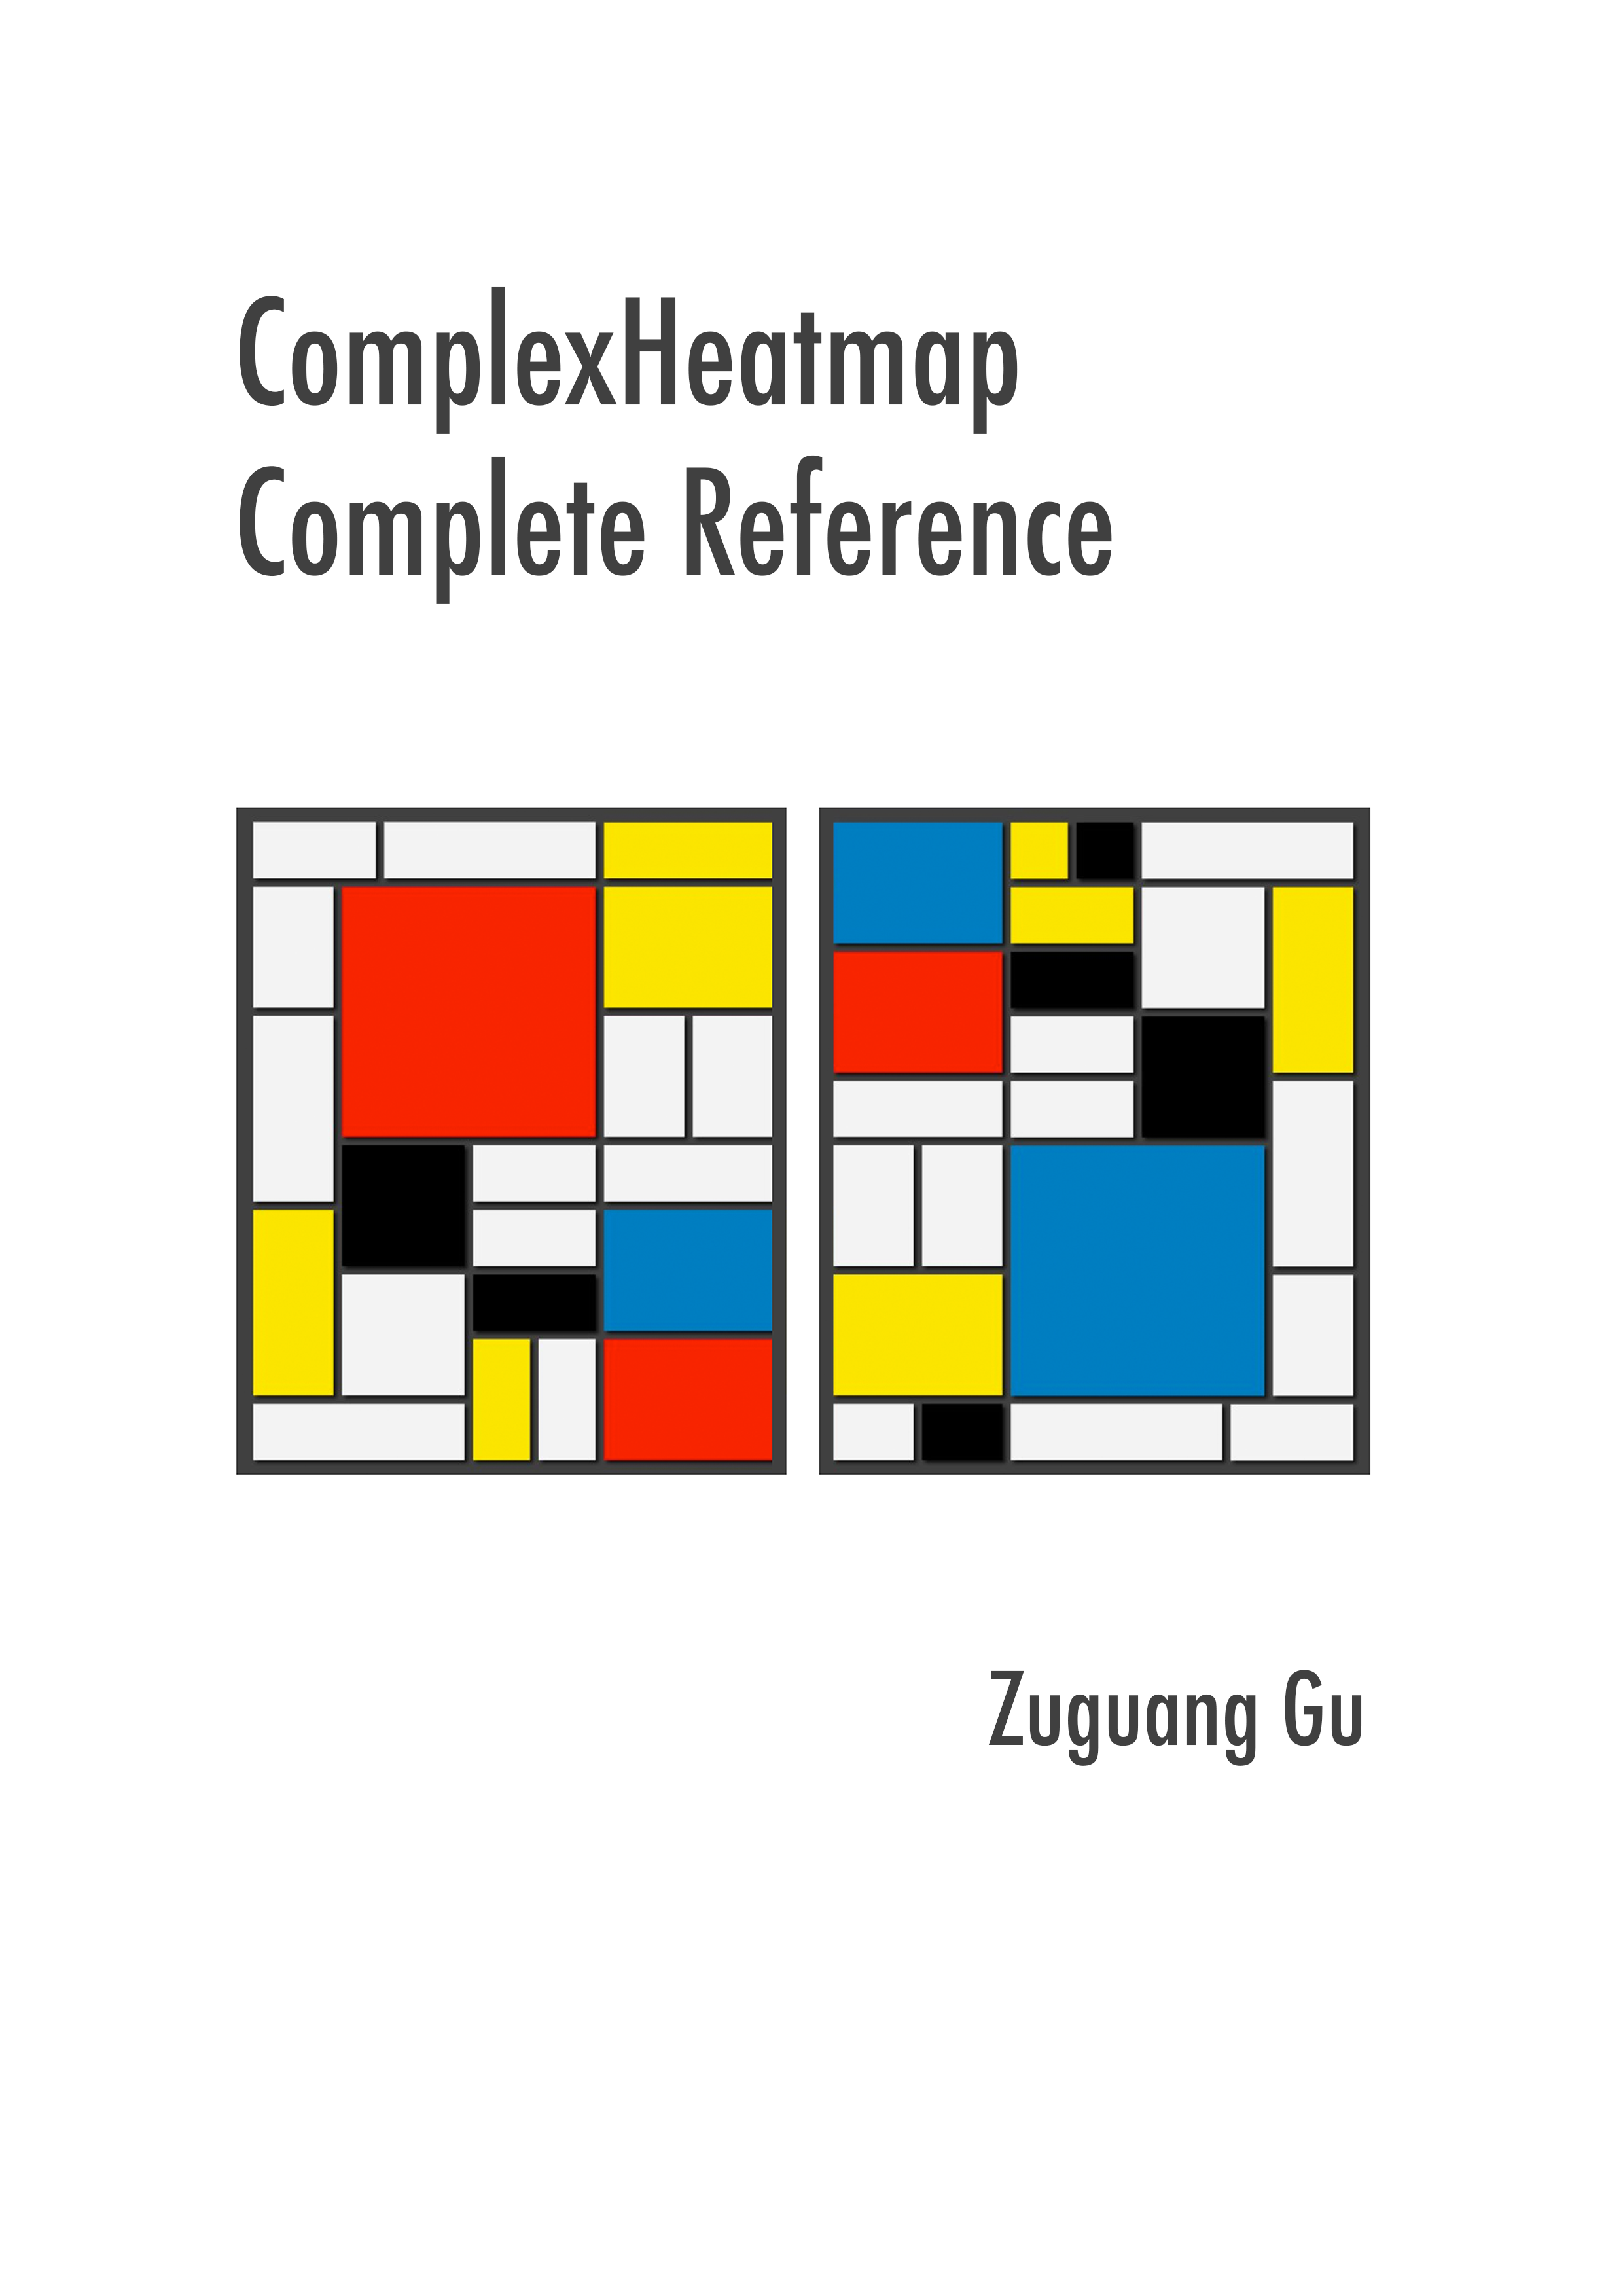
\includegraphics[width=34.44in]{complexheatmap-cover} \end{center}

\chapter{Introduction}\label{introduction}

Complex heatmaps are efficient to visualize associations between
different sources of data sets and reveal potential structures. Here the
\textbf{ComplexHeatmap} package provides a highly flexible way to
arrange multiple heatmaps and supports self-defined annotation graphics.

\section{General design}\label{general-design}

A single heatmap is composed of the heatmap body and the heatmap
components. The heatmap body can be split by rows and columns. The
heatmap components are titles, dendrograms, matrix names and
annotations, which are put on the four sides of the heamap body.

\begin{center}\includegraphics{01-introduction_files/figure-latex/unnamed-chunk-3-1} \end{center}

A heatmap list is concatenation of a list of heatmaps and heatmap
annotations. Surrounding the heatmap list, there are global-level titles
and legends.

One of the important things for the heatmap list is that rows for all
heatmaps and annotations (it is row annotation if the heatmap list is
horizontal.) are all adusted so that the same row in all heatmaps and
annotations corresponds to a same feature.

\begin{center}\includegraphics{01-introduction_files/figure-latex/unnamed-chunk-4-1} \end{center}

The heatmaps and annotations can also be arranged vertically.

\begin{center}\includegraphics{01-introduction_files/figure-latex/unnamed-chunk-5-1} \end{center}

The \textbf{ComplexHeatmap} package is implemented in an object-oriented
way. To describe a heatmap list, there are following classes:

\begin{itemize}
\tightlist
\item
  \texttt{Heatmap} class: a single heatmap containing heatmap body,
  row/column names, titles, dendrograms and column annotations.
\item
  \texttt{HeatmapList} class: a list of heatmaps and heatmap
  annotations.
\item
  \texttt{HeatmapAnnotation} class: defines a list of row annotations
  and column annotations. The heatmap annotations can be components of
  heatmap, also they can be independent as heatmaps.
\end{itemize}

There are also several internal classes:

\begin{itemize}
\tightlist
\item
  \texttt{SingleAnnotation} class: defines a single row annotation or
  column annotation.
\item
  \texttt{ColorMapping} class: mapping from values to colors.
\item
  \texttt{AnnotationFunction} class: construct user-defined annotations.
\end{itemize}

\textbf{ComplexHeatmap} is implemented under \textbf{grid} system, so
users need to know basic \textbf{grid} functionality to get full use of
the package.

\section{A brief description of following
chapters}\label{a-brief-description-of-following-chapters}

\begin{enumerate}
\def\labelenumi{\arabic{enumi}.}
\tightlist
\item
  \href{a-single-heatmap.html}{\textbf{A Single Heatmap}}
\end{enumerate}

This chapter describes the configurations of a single heatmap.

\begin{enumerate}
\def\labelenumi{\arabic{enumi}.}
\setcounter{enumi}{1}
\tightlist
\item
  \protect\hyperlink{heatmap-annotations.html}{\textbf{Heatmap
  Annotations}}
\end{enumerate}

This chapter describes the concept of the heatmap annotation and
demonstrates how to make simple annotations as well as complex
annotations. Also, the chapter explains the difference between column
annotations and row annotations.

\begin{enumerate}
\def\labelenumi{\arabic{enumi}.}
\setcounter{enumi}{2}
\tightlist
\item
  \href{a-list-of-heatmaps.html}{\textbf{A List of Heatmaps}}
\end{enumerate}

This chapter describes how to concatenate a list of heatmaps and
annotations and how adjustment is applied to keep the correspondence of
the heatmaps.

\begin{enumerate}
\def\labelenumi{\arabic{enumi}.}
\setcounter{enumi}{3}
\tightlist
\item
  \href{legends.html}{\textbf{Legends}}
\end{enumerate}

This chapter describes how to configurate the heatmap legends and
annotation legends, also how to create self-defined legends.

\begin{enumerate}
\def\labelenumi{\arabic{enumi}.}
\setcounter{enumi}{4}
\tightlist
\item
  \href{heatmap-decoration.html}{\textbf{Heatmap Decoration}}
\end{enumerate}

This chapter describes methods to add more self-defined graphics to the
heatmaps after the heatmaps are generated.

\begin{enumerate}
\def\labelenumi{\arabic{enumi}.}
\setcounter{enumi}{5}
\tightlist
\item
  \href{oncoprint.html}{\textbf{OncoPrint}}
\end{enumerate}

This chapter describes how to make oncoPrints and how to integrate other
functionalities from \textbf{ComplexHeatmap} to oncoPrints.

\begin{enumerate}
\def\labelenumi{\arabic{enumi}.}
\setcounter{enumi}{6}
\tightlist
\item
  \href{other-high-level-plots.html}{\textbf{Other High-level Plots}}
\end{enumerate}

This chapter describes functions implemented in \textbf{ComplexHeatmap}
for specific use, e.g.~visualizing distributions.

\begin{enumerate}
\def\labelenumi{\arabic{enumi}.}
\setcounter{enumi}{7}
\tightlist
\item
  \href{more-examples.html}{\textbf{More Examples}}
\end{enumerate}

More simulated and real-world examples are shown in this chapter.

\chapter{A single Heatmap}\label{a-single-heatmap}

A single heatmap is the most used way for visualizing the data. Although
``the shining point'' of the \textbf{ComplexHeatmap} package is it can
visualize a list of heatmaps in parallel, as the basic unit of the
heatmap list, it is still very important to have the single heatmap
nicely configured.

First let's generate a random matrix where there are three groups by
columns and three groups by rows:

\begin{Shaded}
\begin{Highlighting}[]
\KeywordTok{set.seed}\NormalTok{(}\DecValTok{123}\NormalTok{)}
\NormalTok{nr1 =}\StringTok{ }\DecValTok{4}\NormalTok{; nr2 =}\StringTok{ }\DecValTok{8}\NormalTok{; nr3 =}\StringTok{ }\DecValTok{6}\NormalTok{; nr =}\StringTok{ }\NormalTok{nr1 }\OperatorTok{+}\StringTok{ }\NormalTok{nr2 }\OperatorTok{+}\StringTok{ }\NormalTok{nr3}
\NormalTok{nc1 =}\StringTok{ }\DecValTok{6}\NormalTok{; nc2 =}\StringTok{ }\DecValTok{8}\NormalTok{; nc3 =}\StringTok{ }\DecValTok{10}\NormalTok{; nc =}\StringTok{ }\NormalTok{nc1 }\OperatorTok{+}\StringTok{ }\NormalTok{nc2 }\OperatorTok{+}\StringTok{ }\NormalTok{nc3}
\NormalTok{mat =}\StringTok{ }\KeywordTok{cbind}\NormalTok{(}\KeywordTok{rbind}\NormalTok{(}\KeywordTok{matrix}\NormalTok{(}\KeywordTok{rnorm}\NormalTok{(nr1}\OperatorTok{*}\NormalTok{nc1, }\DataTypeTok{mean =} \DecValTok{1}\NormalTok{,   }\DataTypeTok{sd =} \FloatTok{0.5}\NormalTok{), }\DataTypeTok{nr =}\NormalTok{ nr1),}
          \KeywordTok{matrix}\NormalTok{(}\KeywordTok{rnorm}\NormalTok{(nr2}\OperatorTok{*}\NormalTok{nc1, }\DataTypeTok{mean =} \DecValTok{0}\NormalTok{,   }\DataTypeTok{sd =} \FloatTok{0.5}\NormalTok{), }\DataTypeTok{nr =}\NormalTok{ nr2),}
          \KeywordTok{matrix}\NormalTok{(}\KeywordTok{rnorm}\NormalTok{(nr3}\OperatorTok{*}\NormalTok{nc1, }\DataTypeTok{mean =} \DecValTok{0}\NormalTok{,   }\DataTypeTok{sd =} \FloatTok{0.5}\NormalTok{), }\DataTypeTok{nr =}\NormalTok{ nr3)),}
    \KeywordTok{rbind}\NormalTok{(}\KeywordTok{matrix}\NormalTok{(}\KeywordTok{rnorm}\NormalTok{(nr1}\OperatorTok{*}\NormalTok{nc2, }\DataTypeTok{mean =} \DecValTok{0}\NormalTok{,   }\DataTypeTok{sd =} \FloatTok{0.5}\NormalTok{), }\DataTypeTok{nr =}\NormalTok{ nr1),}
          \KeywordTok{matrix}\NormalTok{(}\KeywordTok{rnorm}\NormalTok{(nr2}\OperatorTok{*}\NormalTok{nc2, }\DataTypeTok{mean =} \DecValTok{1}\NormalTok{,   }\DataTypeTok{sd =} \FloatTok{0.5}\NormalTok{), }\DataTypeTok{nr =}\NormalTok{ nr2),}
          \KeywordTok{matrix}\NormalTok{(}\KeywordTok{rnorm}\NormalTok{(nr3}\OperatorTok{*}\NormalTok{nc2, }\DataTypeTok{mean =} \DecValTok{0}\NormalTok{,   }\DataTypeTok{sd =} \FloatTok{0.5}\NormalTok{), }\DataTypeTok{nr =}\NormalTok{ nr3)),}
    \KeywordTok{rbind}\NormalTok{(}\KeywordTok{matrix}\NormalTok{(}\KeywordTok{rnorm}\NormalTok{(nr1}\OperatorTok{*}\NormalTok{nc3, }\DataTypeTok{mean =} \FloatTok{0.5}\NormalTok{, }\DataTypeTok{sd =} \FloatTok{0.5}\NormalTok{), }\DataTypeTok{nr =}\NormalTok{ nr1),}
          \KeywordTok{matrix}\NormalTok{(}\KeywordTok{rnorm}\NormalTok{(nr2}\OperatorTok{*}\NormalTok{nc3, }\DataTypeTok{mean =} \FloatTok{0.5}\NormalTok{, }\DataTypeTok{sd =} \FloatTok{0.5}\NormalTok{), }\DataTypeTok{nr =}\NormalTok{ nr2),}
          \KeywordTok{matrix}\NormalTok{(}\KeywordTok{rnorm}\NormalTok{(nr3}\OperatorTok{*}\NormalTok{nc3, }\DataTypeTok{mean =} \DecValTok{1}\NormalTok{,   }\DataTypeTok{sd =} \FloatTok{0.5}\NormalTok{), }\DataTypeTok{nr =}\NormalTok{ nr3))}
\NormalTok{   )}
\NormalTok{mat =}\StringTok{ }\NormalTok{mat[}\KeywordTok{sample}\NormalTok{(nr, nr), }\KeywordTok{sample}\NormalTok{(nc, nc)] }\CommentTok{# random shuffle rows and columns}
\KeywordTok{rownames}\NormalTok{(mat) =}\StringTok{ }\KeywordTok{paste0}\NormalTok{(}\StringTok{"row"}\NormalTok{, }\KeywordTok{seq_len}\NormalTok{(nr))}
\KeywordTok{colnames}\NormalTok{(mat) =}\StringTok{ }\KeywordTok{paste0}\NormalTok{(}\StringTok{"column"}\NormalTok{, }\KeywordTok{seq_len}\NormalTok{(nc))}
\end{Highlighting}
\end{Shaded}

Following command contains the minimal argument for the
\texttt{Heatmap()} function which just visualizes the matrix as a
heatmap with default settings. Very similar as other heatmap tools, it
draws the dendrograms, the row/column names and the heatmap legend. The
default color schema is ``blue-white-red'' which is mapped to the
minimal-mean-maximal values in the matrix. The title for the legend is
assigned by an internal index number.

\begin{Shaded}
\begin{Highlighting}[]
\KeywordTok{Heatmap}\NormalTok{(mat)}
\end{Highlighting}
\end{Shaded}

\begin{center}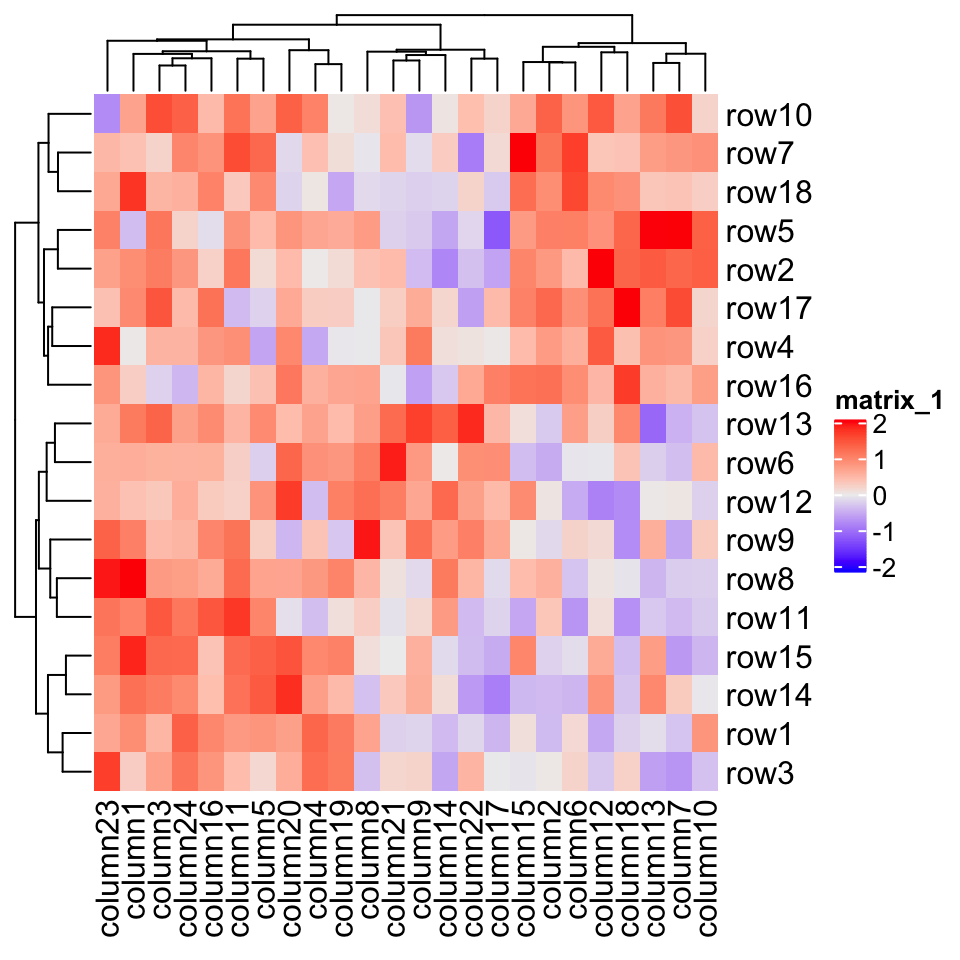
\includegraphics{02-single_heatmap_files/figure-latex/default-1} \end{center}

The title for the legend is taken from the ``name'' of the heatmap by
default. Each heatmap has a name which is like a unique identifier for
the heatmap, which is important when you have a list of heatmaps. In
later chapters, you will find the heatmap name is used for setting the
``main heatmap'' and is used for decoration of heatmaps. If the name is
not assigned, an internal name is assigned to the heatmap in a form of
\texttt{matrix\_\%d}. In following examples in this chapter, we give the
name \texttt{mat} to the heatmap (for which you will see the change of
the legend in the next plot).

\section{Colors}\label{colors}

For heatmap visualization, colors are the major representation of the
data matrix. In most cases, the heatmap visualizes a matrix with
continuous numeric values. In this case, users should provide a color
mapping function. A color mapping function should accept a vector of
values and return a vector of corresponding colors. \textbf{Users should
always use \texttt{circlize::colorRamp2()} function to generate the
color mapping function}. The two arguments for \texttt{colorRamp2()} is
a vector of break values and a vector of corresponding colors.
\texttt{colorRamp2()} linearly interpolates colors in every interval
through LAB color space. Also using \texttt{colorRamp2()} helps to
generate a legend with proper tick marks.

In following example, values between -2 and 2 are linearly interpolated
to get corresponding colors, values larger than 2 are all mapped to red
and values less than -2 are all mapped to green.

\begin{Shaded}
\begin{Highlighting}[]
\KeywordTok{library}\NormalTok{(circlize)}
\NormalTok{col_fun =}\StringTok{ }\KeywordTok{colorRamp2}\NormalTok{(}\KeywordTok{c}\NormalTok{(}\OperatorTok{-}\DecValTok{2}\NormalTok{, }\DecValTok{0}\NormalTok{, }\DecValTok{2}\NormalTok{), }\KeywordTok{c}\NormalTok{(}\StringTok{"green"}\NormalTok{, }\StringTok{"white"}\NormalTok{, }\StringTok{"red"}\NormalTok{))}
\KeywordTok{col_fun}\NormalTok{(}\KeywordTok{seq}\NormalTok{(}\OperatorTok{-}\DecValTok{3}\NormalTok{, }\DecValTok{3}\NormalTok{))}
\end{Highlighting}
\end{Shaded}

\begin{verbatim}
## [1] "#00FF00FF" "#00FF00FF" "#B1FF9AFF" "#FFFFFFFF" "#FF9E81FF" "#FF0000FF"
## [7] "#FF0000FF"
\end{verbatim}

\begin{Shaded}
\begin{Highlighting}[]
\KeywordTok{Heatmap}\NormalTok{(mat, }\DataTypeTok{name =} \StringTok{"mat"}\NormalTok{, }\DataTypeTok{col =}\NormalTok{ col_fun)}
\end{Highlighting}
\end{Shaded}

\begin{center}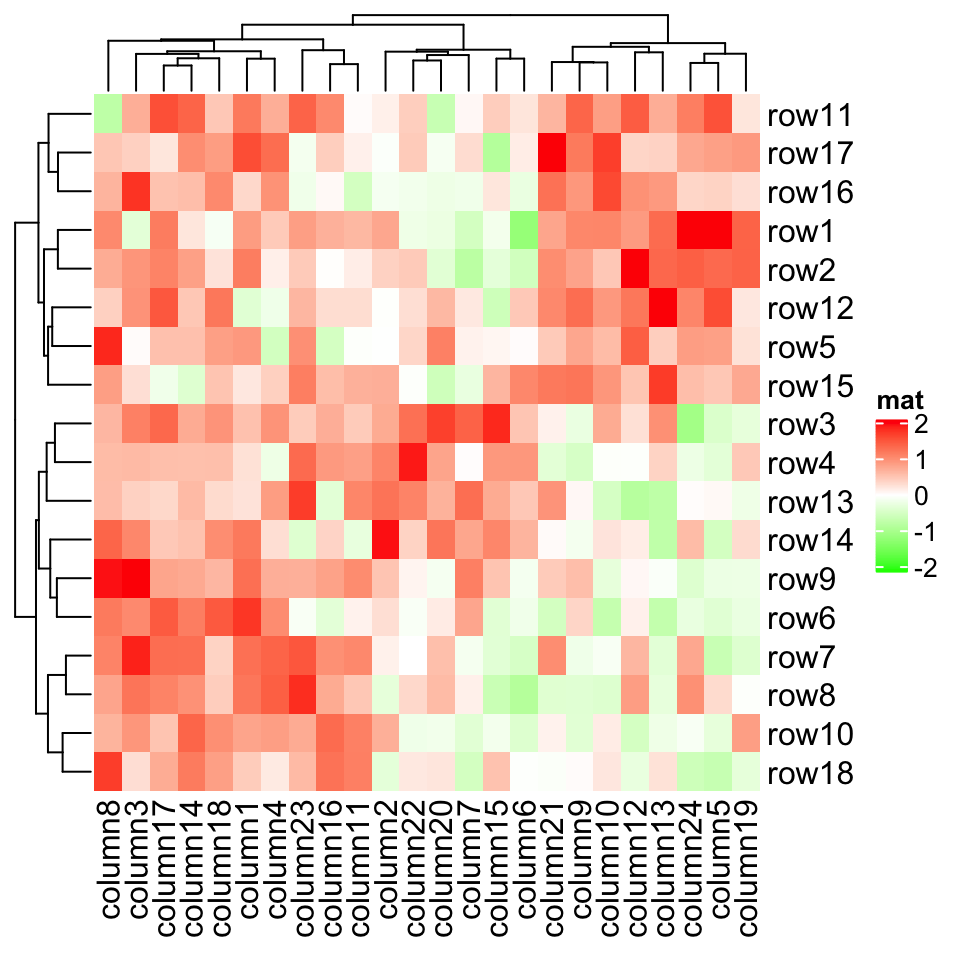
\includegraphics{02-single_heatmap_files/figure-latex/unnamed-chunk-2-1} \end{center}

As you can see, the color mapping function exactly maps negative values
to green and positive values to red, even when the distribution of
negative values and positive values are not centric to zero. Also this
color mapping function is not affected by outliers. In following plot,
the clustering is heavily affected by the outlier but not the color
mapping.

\begin{Shaded}
\begin{Highlighting}[]
\NormalTok{mat2 =}\StringTok{ }\NormalTok{mat}
\NormalTok{mat2[}\DecValTok{1}\NormalTok{, }\DecValTok{1}\NormalTok{] =}\StringTok{ }\DecValTok{100000}
\KeywordTok{Heatmap}\NormalTok{(mat2, }\DataTypeTok{name =} \StringTok{"mat"}\NormalTok{, }\DataTypeTok{col =}\NormalTok{ col_fun)}
\end{Highlighting}
\end{Shaded}

\begin{center}\includegraphics{02-single_heatmap_files/figure-latex/unnamed-chunk-3-1} \end{center}

More importantly, \texttt{colorRamp2()} makes colors in multiple
heatmaps comparible if they are set with a same color mapping function.

If the matrix is continuous, you can simply provide a vector of colors
and colors will be linearly interpolated. But remember this method is
not robust to outliers because the mapping starts from the minimal value
in the matrix and ends with the maximal value. Following color mapping
setting is identical to
\texttt{colorRamp2(seq(min(mat),\ max(mat),\ length\ =\ 10),\ rev(rainbow(10)))}.

\begin{Shaded}
\begin{Highlighting}[]
\KeywordTok{Heatmap}\NormalTok{(mat, }\DataTypeTok{name =} \StringTok{"mat"}\NormalTok{, }\DataTypeTok{col =} \KeywordTok{rev}\NormalTok{(}\KeywordTok{rainbow}\NormalTok{(}\DecValTok{10}\NormalTok{)))}
\end{Highlighting}
\end{Shaded}

\begin{center}\includegraphics{02-single_heatmap_files/figure-latex/unnamed-chunk-4-1} \end{center}

If the matrix contains discrete values (either numeric or character),
colors should be specified as a named vector to make it possible for the
mapping from discrete values to colors. If there is no name for the
color, the order of colors corresponds to the order of
\texttt{unique(mat)}. Note now the legend is generated from the color
mapping vector.

Following sets colors for a discrete numeric matrix (you don't need to
convert it to a character matrix).

\begin{Shaded}
\begin{Highlighting}[]
\NormalTok{discrete_mat =}\StringTok{ }\KeywordTok{matrix}\NormalTok{(}\KeywordTok{sample}\NormalTok{(}\DecValTok{1}\OperatorTok{:}\DecValTok{4}\NormalTok{, }\DecValTok{100}\NormalTok{, }\DataTypeTok{replace =} \OtherTok{TRUE}\NormalTok{), }\DecValTok{10}\NormalTok{, }\DecValTok{10}\NormalTok{)}
\NormalTok{colors =}\StringTok{ }\KeywordTok{structure}\NormalTok{(}\DecValTok{1}\OperatorTok{:}\DecValTok{4}\NormalTok{, }\DataTypeTok{names =} \KeywordTok{c}\NormalTok{(}\StringTok{"1"}\NormalTok{, }\StringTok{"2"}\NormalTok{, }\StringTok{"3"}\NormalTok{, }\StringTok{"4"}\NormalTok{)) }\CommentTok{# black, red, green, blue}
\KeywordTok{Heatmap}\NormalTok{(discrete_mat, }\DataTypeTok{name =} \StringTok{"mat"}\NormalTok{, }\DataTypeTok{col =}\NormalTok{ colors)}
\end{Highlighting}
\end{Shaded}

\begin{center}\includegraphics{02-single_heatmap_files/figure-latex/unnamed-chunk-5-1} \end{center}

Or a character matrix:

\begin{Shaded}
\begin{Highlighting}[]
\NormalTok{discrete_mat =}\StringTok{ }\KeywordTok{matrix}\NormalTok{(}\KeywordTok{sample}\NormalTok{(letters[}\DecValTok{1}\OperatorTok{:}\DecValTok{4}\NormalTok{], }\DecValTok{100}\NormalTok{, }\DataTypeTok{replace =} \OtherTok{TRUE}\NormalTok{), }\DecValTok{10}\NormalTok{, }\DecValTok{10}\NormalTok{)}
\NormalTok{colors =}\StringTok{ }\KeywordTok{structure}\NormalTok{(}\DecValTok{1}\OperatorTok{:}\DecValTok{4}\NormalTok{, }\DataTypeTok{names =}\NormalTok{ letters[}\DecValTok{1}\OperatorTok{:}\DecValTok{4}\NormalTok{])}
\KeywordTok{Heatmap}\NormalTok{(discrete_mat, }\DataTypeTok{name =} \StringTok{"mat"}\NormalTok{, }\DataTypeTok{col =}\NormalTok{ colors)}
\end{Highlighting}
\end{Shaded}

\begin{center}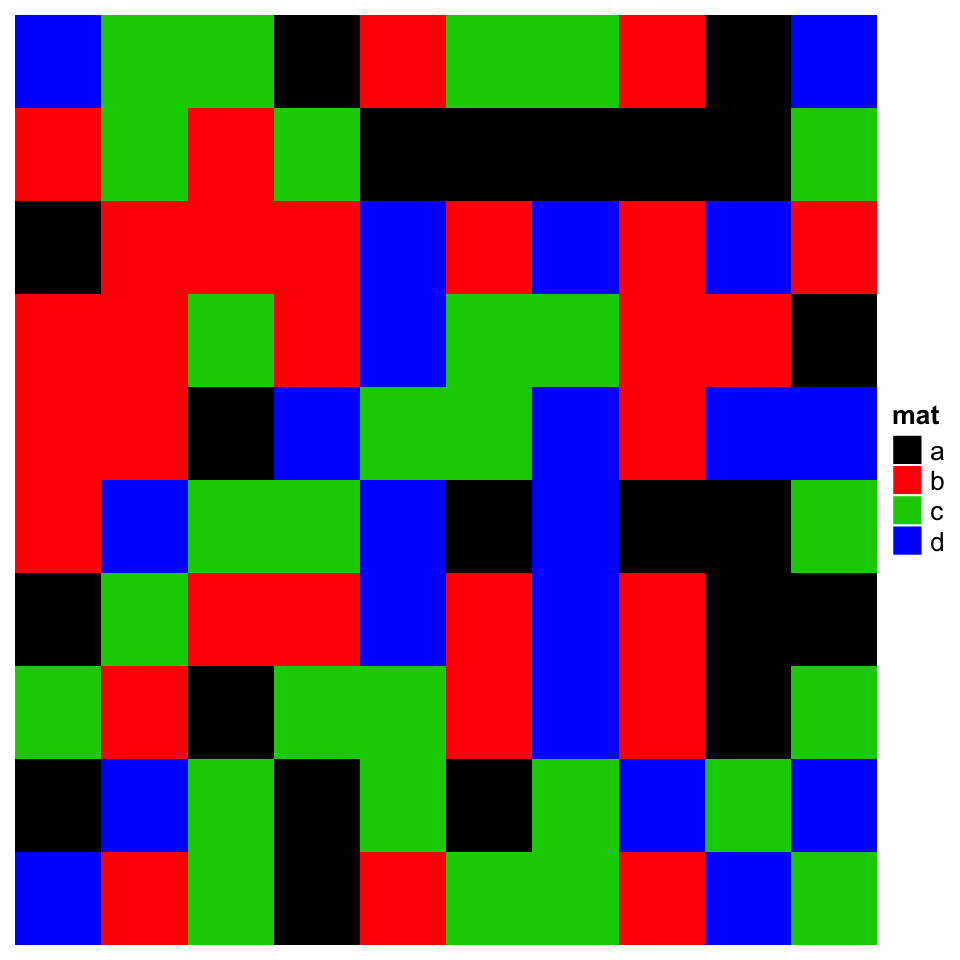
\includegraphics{02-single_heatmap_files/figure-latex/discrete_character_matrix-1} \end{center}

As you see in the two above examples, for the numeric matrix (no matter
the color is continuous mapping or discrete mapping), by default
clustering is applied on both dimensions while for character matrix,
clustering is turned off (but you can still clustering a character
matrix if you provide a proper distance metric for two character
vectors, see example in Section \ref{distance-methods}).

\texttt{NA} is allowed in the matrix. You can control the color of
\texttt{NA} by \texttt{na\_col} argument (by default it is grey for
\texttt{NA}). \textbf{The matrix that contains \texttt{NA} can also be
clustered by \texttt{Heatmap()}.}

Note the \texttt{NA} value is not presended in the legend.

\begin{Shaded}
\begin{Highlighting}[]
\NormalTok{mat_with_na =}\StringTok{ }\NormalTok{mat}
\NormalTok{na_index =}\StringTok{ }\KeywordTok{sample}\NormalTok{(}\KeywordTok{c}\NormalTok{(}\OtherTok{TRUE}\NormalTok{, }\OtherTok{FALSE}\NormalTok{), }\KeywordTok{nrow}\NormalTok{(mat)}\OperatorTok{*}\KeywordTok{ncol}\NormalTok{(mat), }\DataTypeTok{replace =} \OtherTok{TRUE}\NormalTok{, }\DataTypeTok{prob =} \KeywordTok{c}\NormalTok{(}\DecValTok{1}\NormalTok{, }\DecValTok{9}\NormalTok{))}
\NormalTok{mat_with_na[na_index] =}\StringTok{ }\OtherTok{NA}
\KeywordTok{Heatmap}\NormalTok{(mat_with_na, }\DataTypeTok{name =} \StringTok{"mat"}\NormalTok{, }\DataTypeTok{na_col =} \StringTok{"black"}\NormalTok{)}
\end{Highlighting}
\end{Shaded}

\begin{center}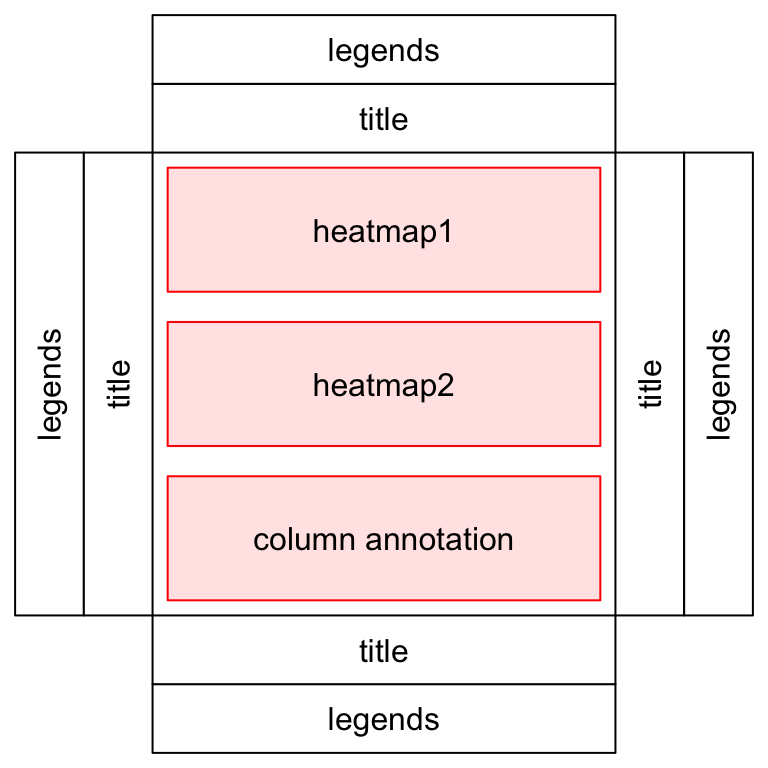
\includegraphics{02-single_heatmap_files/figure-latex/unnamed-chunk-6-1} \end{center}

Color space is important for interpolating colors. By default, colors
are linearly interpolated in
\href{https://en.wikipedia.org/wiki/Lab_color_space}{LAB color space},
but you can select the color space in \texttt{colorRamp2()} function.
Compare following two plots. Can you see the difference?

\begin{Shaded}
\begin{Highlighting}[]
\NormalTok{f1 =}\StringTok{ }\KeywordTok{colorRamp2}\NormalTok{(}\KeywordTok{seq}\NormalTok{(}\KeywordTok{min}\NormalTok{(mat), }\KeywordTok{max}\NormalTok{(mat), }\DataTypeTok{length =} \DecValTok{3}\NormalTok{), }\KeywordTok{c}\NormalTok{(}\StringTok{"blue"}\NormalTok{, }\StringTok{"#EEEEEE"}\NormalTok{, }\StringTok{"red"}\NormalTok{))}
\NormalTok{f2 =}\StringTok{ }\KeywordTok{colorRamp2}\NormalTok{(}\KeywordTok{seq}\NormalTok{(}\KeywordTok{min}\NormalTok{(mat), }\KeywordTok{max}\NormalTok{(mat), }\DataTypeTok{length =} \DecValTok{3}\NormalTok{), }\KeywordTok{c}\NormalTok{(}\StringTok{"blue"}\NormalTok{, }\StringTok{"#EEEEEE"}\NormalTok{, }\StringTok{"red"}\NormalTok{), }
    \DataTypeTok{space =} \StringTok{"RGB"}\NormalTok{)}
\KeywordTok{Heatmap}\NormalTok{(mat, }\DataTypeTok{name =} \StringTok{"mat1"}\NormalTok{, }\DataTypeTok{col =}\NormalTok{ f1, }\DataTypeTok{column_title =} \StringTok{"LAB color space"}\NormalTok{)}
\KeywordTok{Heatmap}\NormalTok{(mat, }\DataTypeTok{name =} \StringTok{"mat2"}\NormalTok{, }\DataTypeTok{col =}\NormalTok{ f2, }\DataTypeTok{column_title =} \StringTok{"RGB color space"}\NormalTok{)}
\end{Highlighting}
\end{Shaded}

\begin{center}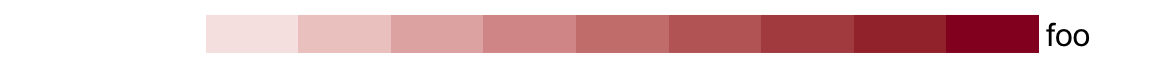
\includegraphics{02-single_heatmap_files/figure-latex/unnamed-chunk-8-1} \end{center}

In following figures, corresponding values change evenly on the folded
lines, you can see how colors change under different color spaces (the
plot is made by
\href{https://bioconductor.org/packages/release/bioc/html/HilbertCurve.html}{\textbf{HilbertCurve}
package}).

\begin{center}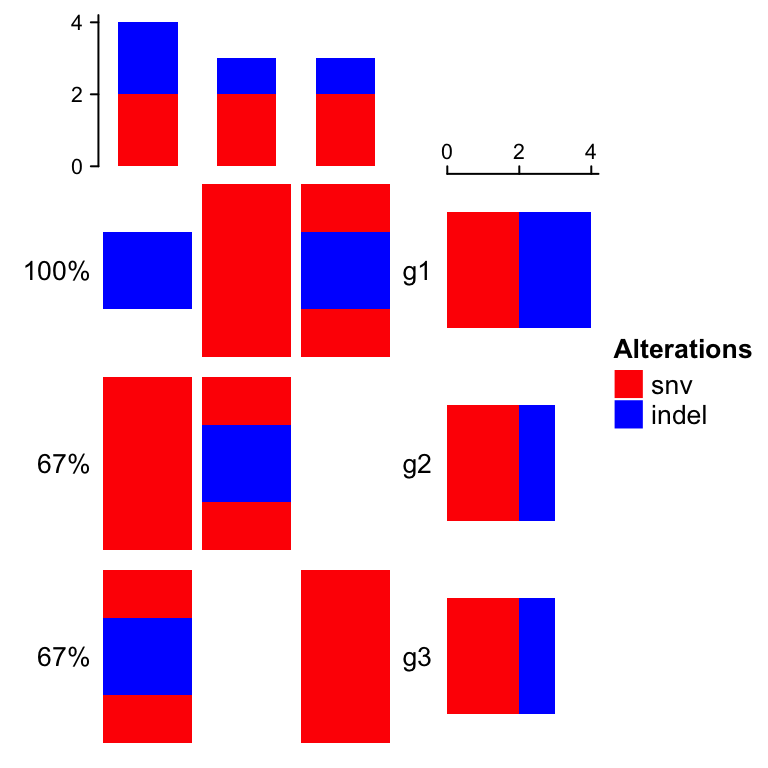
\includegraphics{02-single_heatmap_files/figure-latex/unnamed-chunk-9-1} \end{center}

\begin{center}\includegraphics{02-single_heatmap_files/figure-latex/unnamed-chunk-9-2} \end{center}

Last but not the least, colors for the heatmap borders can be set by the
\texttt{border} and \texttt{rect\_gp} arguments. \texttt{border}
controls the global border of the heatmap body and \texttt{rect\_gp}
controls the border of the grids in the heatmap.

The value of \texttt{border} can be logical (\texttt{TRUE} corresponds
to \texttt{black}) or a character of color (e.g. \texttt{red}).

\texttt{rect\_gp} is a \texttt{gpar} object which means you can only set
it by \texttt{grid::gpar()}. Since the filled color is already
controlled by the heatmap color mapping, you can only set the
\texttt{col} parameter in \texttt{gpar()} to control the border of the
heatmap grids.

\begin{Shaded}
\begin{Highlighting}[]
\KeywordTok{Heatmap}\NormalTok{(mat, }\DataTypeTok{name =} \StringTok{"mat"}\NormalTok{, }\DataTypeTok{border =} \OtherTok{TRUE}\NormalTok{)}
\end{Highlighting}
\end{Shaded}

\begin{center}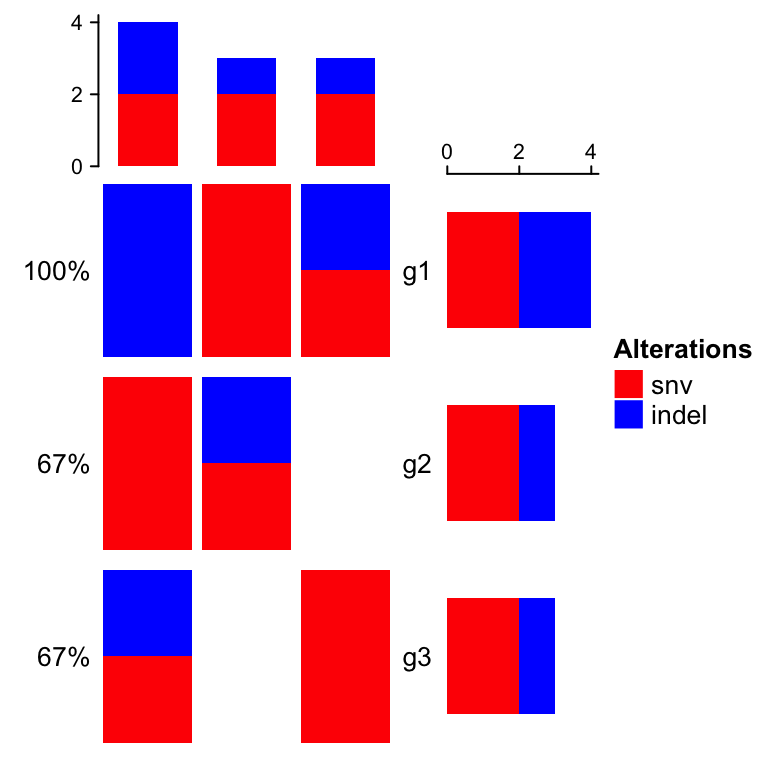
\includegraphics{02-single_heatmap_files/figure-latex/unnamed-chunk-10-1} \end{center}

\begin{Shaded}
\begin{Highlighting}[]
\KeywordTok{Heatmap}\NormalTok{(mat, }\DataTypeTok{name =} \StringTok{"mat"}\NormalTok{, }\DataTypeTok{rect_gp =} \KeywordTok{gpar}\NormalTok{(}\DataTypeTok{col =} \StringTok{"white"}\NormalTok{, }\DataTypeTok{lwd =} \DecValTok{2}\NormalTok{))}
\end{Highlighting}
\end{Shaded}

\begin{center}\includegraphics{02-single_heatmap_files/figure-latex/unnamed-chunk-10-2} \end{center}

\section{Titles}\label{heatmap-titles}

The title of the heatmap basically tells what the plot is about. In
\textbf{ComplexHeatmap} package, you can set heatmap title either by the
row or/and by the column. Note at a same time you can only put
e.g.~column title either on the top or at the bottom of the heatmap.

The graphic parameters can be set by \texttt{row\_title\_gp} and
\texttt{column\_title\_gp} respectively. Please remember you should use
\texttt{gpar()} to specify graphic parameters.

\begin{Shaded}
\begin{Highlighting}[]
\KeywordTok{Heatmap}\NormalTok{(mat, }\DataTypeTok{name =} \StringTok{"mat"}\NormalTok{, }\DataTypeTok{column_title =} \StringTok{"I am a column title"}\NormalTok{, }
    \DataTypeTok{row_title =} \StringTok{"I am a row title"}\NormalTok{)}
\end{Highlighting}
\end{Shaded}

\begin{center}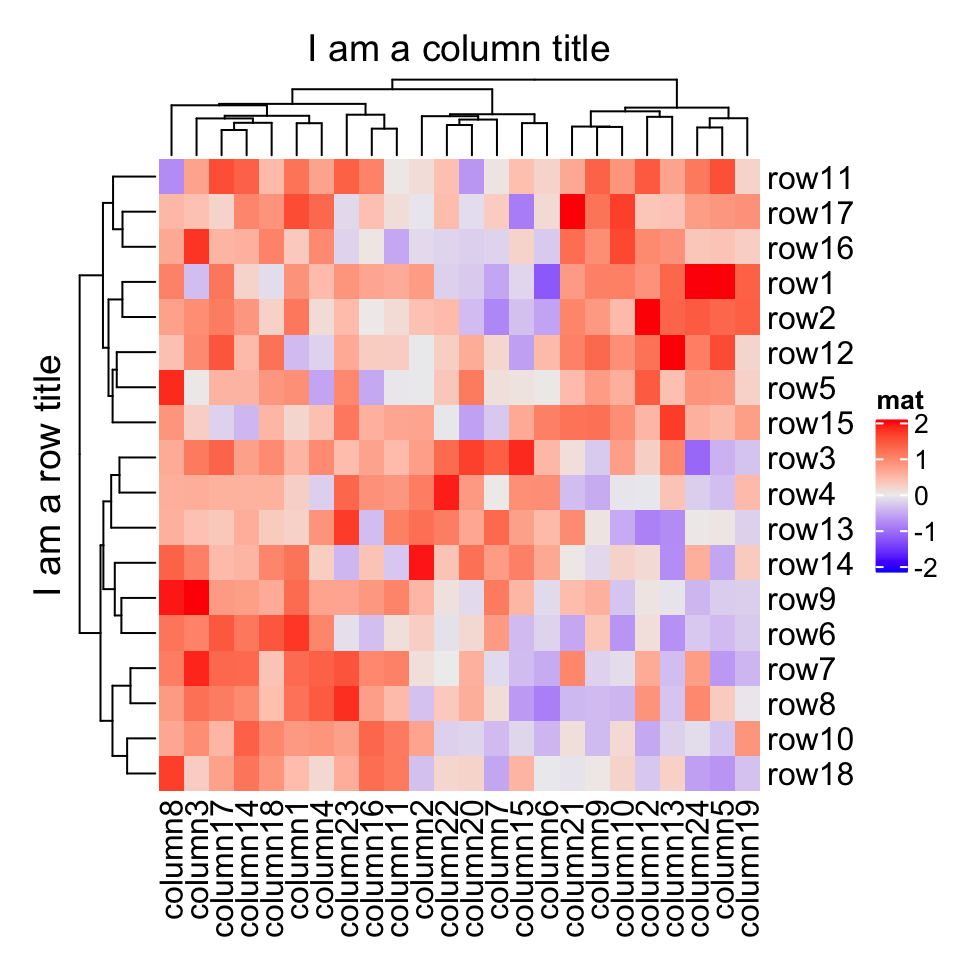
\includegraphics{02-single_heatmap_files/figure-latex/row_column_title-1} \end{center}

\begin{Shaded}
\begin{Highlighting}[]
\KeywordTok{Heatmap}\NormalTok{(mat, }\DataTypeTok{name =} \StringTok{"mat"}\NormalTok{, }\DataTypeTok{column_title =} \StringTok{"I am a column title at the bottom"}\NormalTok{, }
    \DataTypeTok{column_title_side =} \StringTok{"bottom"}\NormalTok{)}
\end{Highlighting}
\end{Shaded}

\begin{center}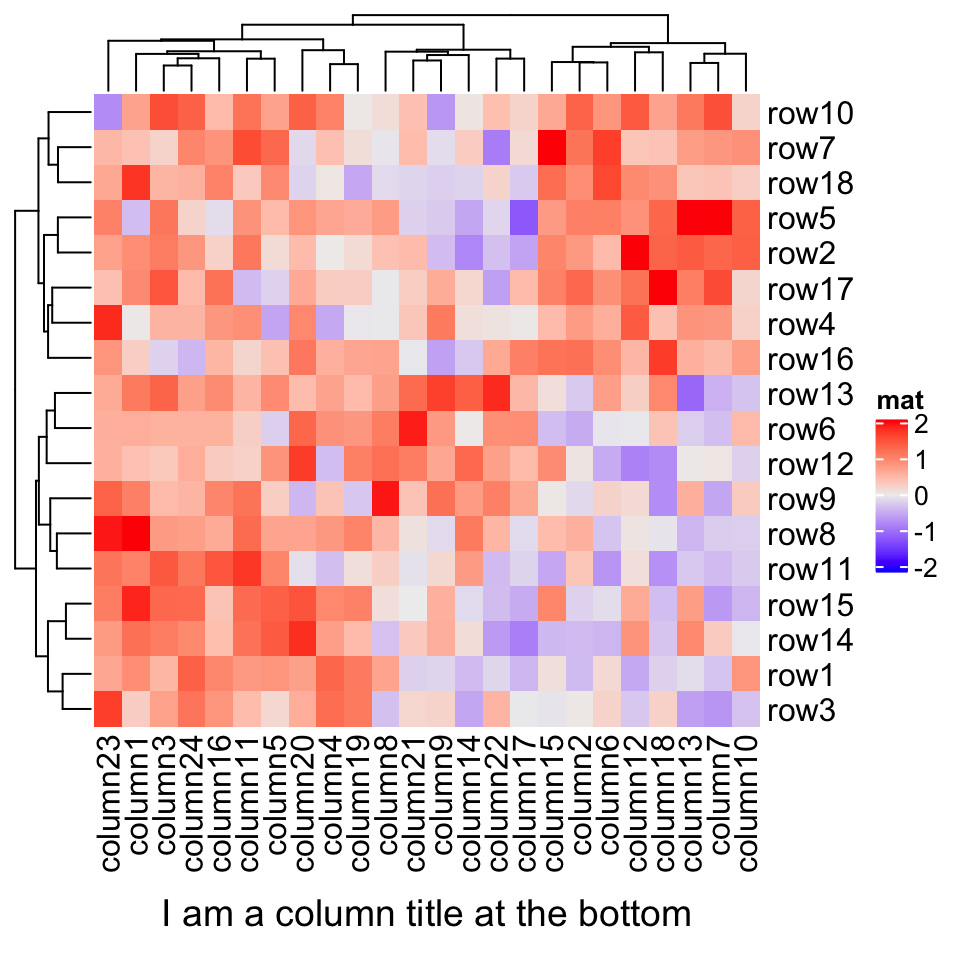
\includegraphics{02-single_heatmap_files/figure-latex/row_column_title-2} \end{center}

\begin{Shaded}
\begin{Highlighting}[]
\KeywordTok{Heatmap}\NormalTok{(mat, }\DataTypeTok{name =} \StringTok{"mat"}\NormalTok{, }\DataTypeTok{column_title =} \StringTok{"I am a big column title"}\NormalTok{, }
    \DataTypeTok{column_title_gp =} \KeywordTok{gpar}\NormalTok{(}\DataTypeTok{fontsize =} \DecValTok{20}\NormalTok{, }\DataTypeTok{fontface =} \StringTok{"bold"}\NormalTok{))}
\end{Highlighting}
\end{Shaded}

\begin{center}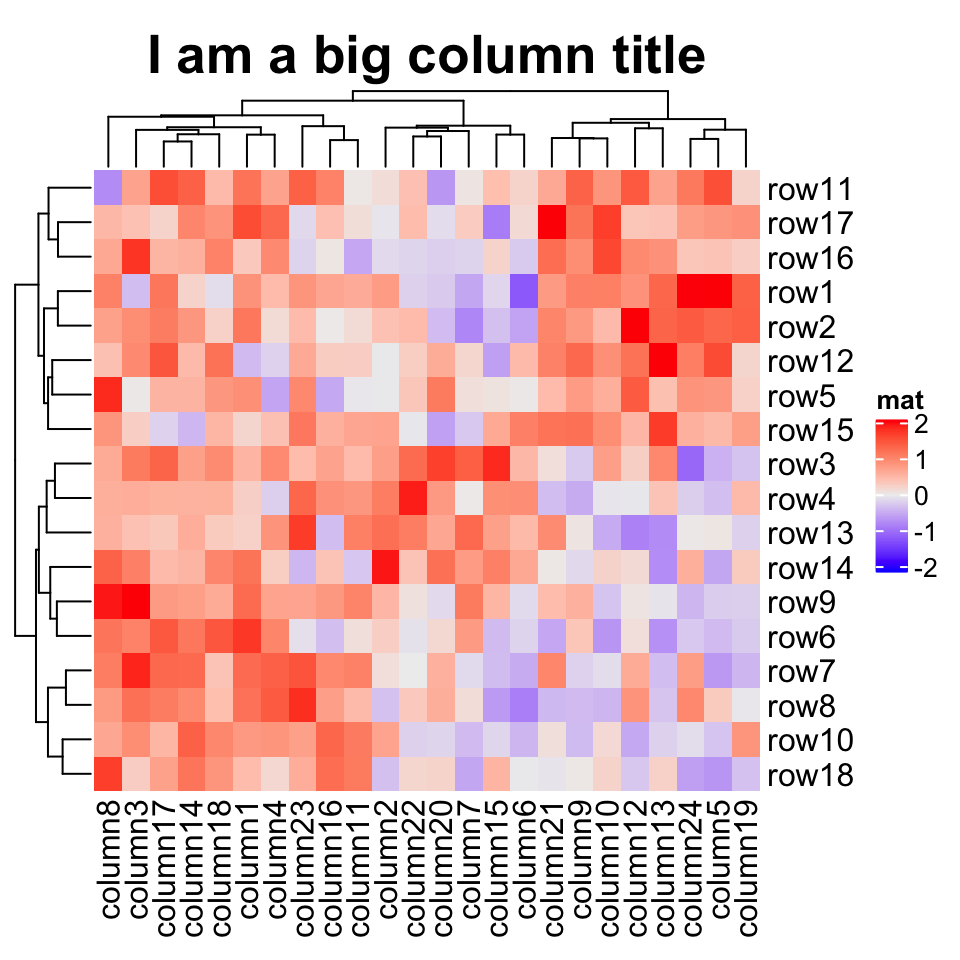
\includegraphics{02-single_heatmap_files/figure-latex/row_column_title-3} \end{center}

Rotations for titles can be set by \texttt{row\_title\_rot} and
\texttt{column\_title\_rot}, but only horizontal and vertical rotations
are allowed.

\begin{Shaded}
\begin{Highlighting}[]
\KeywordTok{Heatmap}\NormalTok{(mat, }\DataTypeTok{name =} \StringTok{"mat"}\NormalTok{, }\DataTypeTok{row_title =} \StringTok{"row title"}\NormalTok{, }\DataTypeTok{row_title_rot =} \DecValTok{0}\NormalTok{)}
\end{Highlighting}
\end{Shaded}

\begin{center}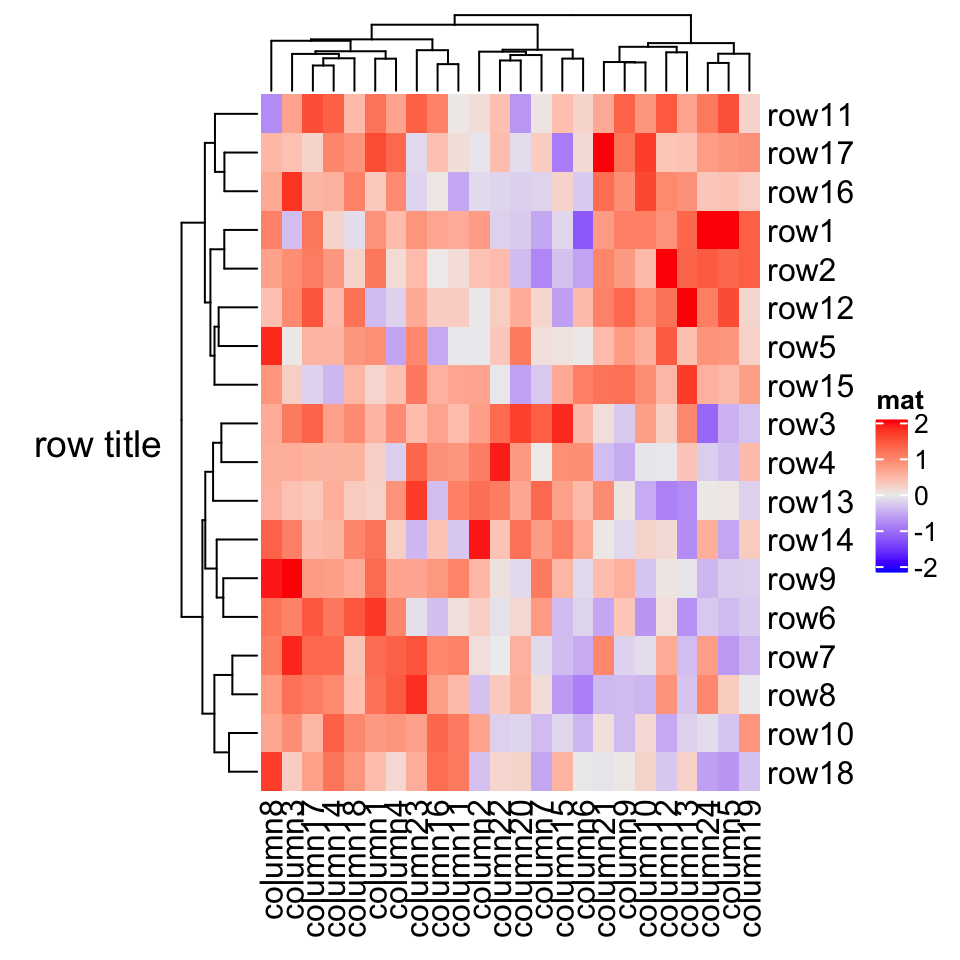
\includegraphics{02-single_heatmap_files/figure-latex/title_rotation-1} \end{center}

Row or column title supports as a template which is used when rows or
columns are split in the heatmap (because there will be multiple
row/column titles). This functionality is introduced in Section
\ref{heatmap-split}. A quick example would be:

\begin{Shaded}
\begin{Highlighting}[]
\CommentTok{# code only for demonstration}
\CommentTok{# row title would be cluster_1 and cluster_2}
\KeywordTok{Heatmap}\NormalTok{(mat, }\DataTypeTok{name =} \StringTok{"mat"}\NormalTok{, }\DataTypeTok{row_km =} \DecValTok{2}\NormalTok{, }\DataTypeTok{row_title =} \StringTok{"cluster_%s"}\NormalTok{)}
\end{Highlighting}
\end{Shaded}

You can set \texttt{fill} parameter in \texttt{row\_title\_gp} and
\texttt{column\_title\_gp} to set the background color of titles.

\begin{Shaded}
\begin{Highlighting}[]
\KeywordTok{Heatmap}\NormalTok{(mat, }\DataTypeTok{name =} \StringTok{"mat"}\NormalTok{, }\DataTypeTok{column_title =} \StringTok{"I am a column title"}\NormalTok{, }
    \DataTypeTok{column_title_gp =} \KeywordTok{gpar}\NormalTok{(}\DataTypeTok{fill =} \StringTok{"red"}\NormalTok{, }\DataTypeTok{col =} \StringTok{"white"}\NormalTok{))}
\end{Highlighting}
\end{Shaded}

\begin{center}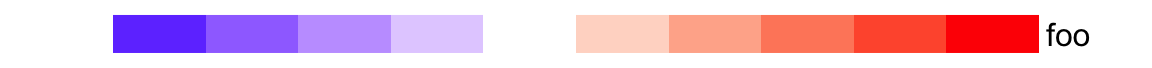
\includegraphics{02-single_heatmap_files/figure-latex/unnamed-chunk-12-1} \end{center}

\section{Clustering}\label{clustering}

Clustering might be the key component of the heatmap visualization. In
\textbf{ComplexHeatmap} package, hierarchical clustering is supported
with great flexibility. You can specify the clustering either by:

\begin{itemize}
\tightlist
\item
  a pre-defined distance method (e.g. \texttt{"eulidean"} or
  \texttt{"pearson"}),
\item
  a distance function,
\item
  a object that already contains clustering (a \texttt{hclust} or
  \texttt{dendrogram} object or object that can be coerced to
  \texttt{hclust} or \texttt{dendrogram} class),
\item
  a clustering function.
\end{itemize}

It is also possible to render the dendrograms with different colors and
styles for different branches for better revealing structures of your
data (e.g.~by \texttt{dendextend::color\_branches()}).

First, there are general settings for the clustering, e.g.~whether apply
clustering or show dendrograms, the side of the dendrograms and heights
of the dendrograms.

\begin{Shaded}
\begin{Highlighting}[]
\KeywordTok{Heatmap}\NormalTok{(mat, }\DataTypeTok{name =} \StringTok{"mat"}\NormalTok{, }\DataTypeTok{cluster_rows =} \OtherTok{FALSE}\NormalTok{) }\CommentTok{# turn off row clustering}
\end{Highlighting}
\end{Shaded}

\begin{center}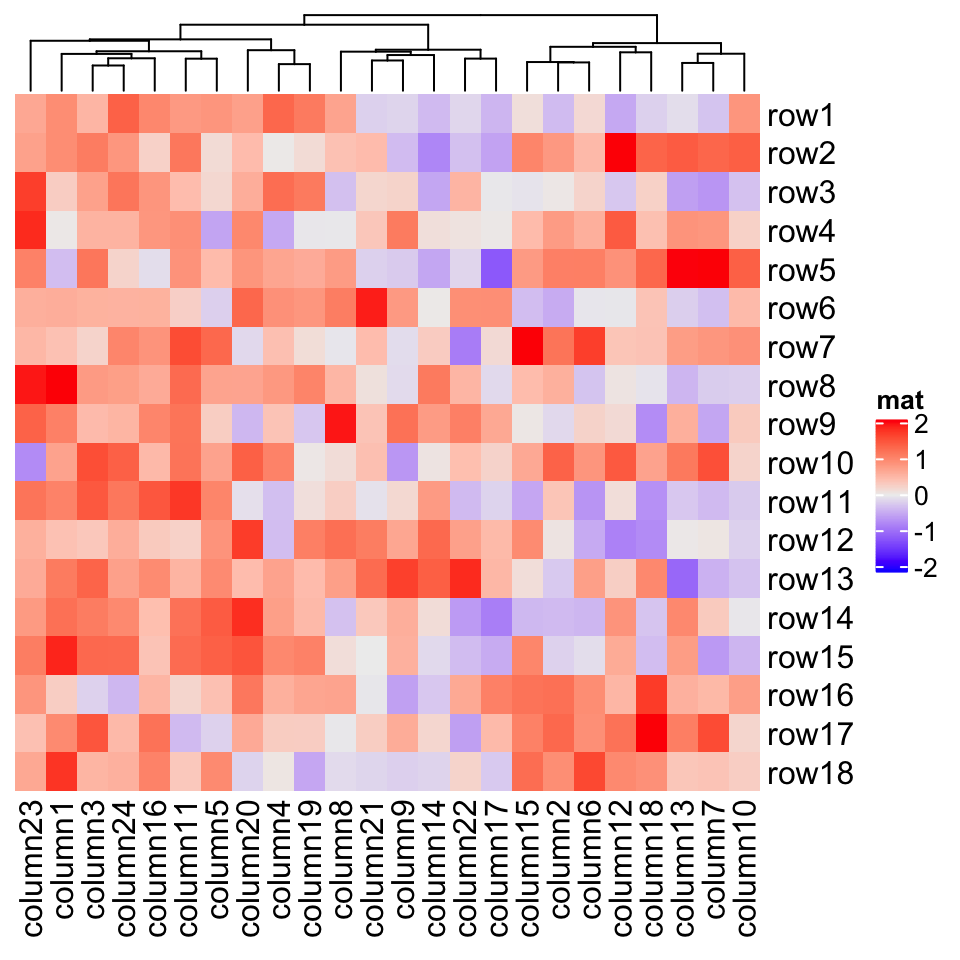
\includegraphics{02-single_heatmap_files/figure-latex/cluster_basic-1} \end{center}

\begin{Shaded}
\begin{Highlighting}[]
\KeywordTok{Heatmap}\NormalTok{(mat, }\DataTypeTok{name =} \StringTok{"mat"}\NormalTok{, }\DataTypeTok{show_column_dend =} \OtherTok{FALSE}\NormalTok{) }\CommentTok{# hide column dendrogram}
\end{Highlighting}
\end{Shaded}

\begin{center}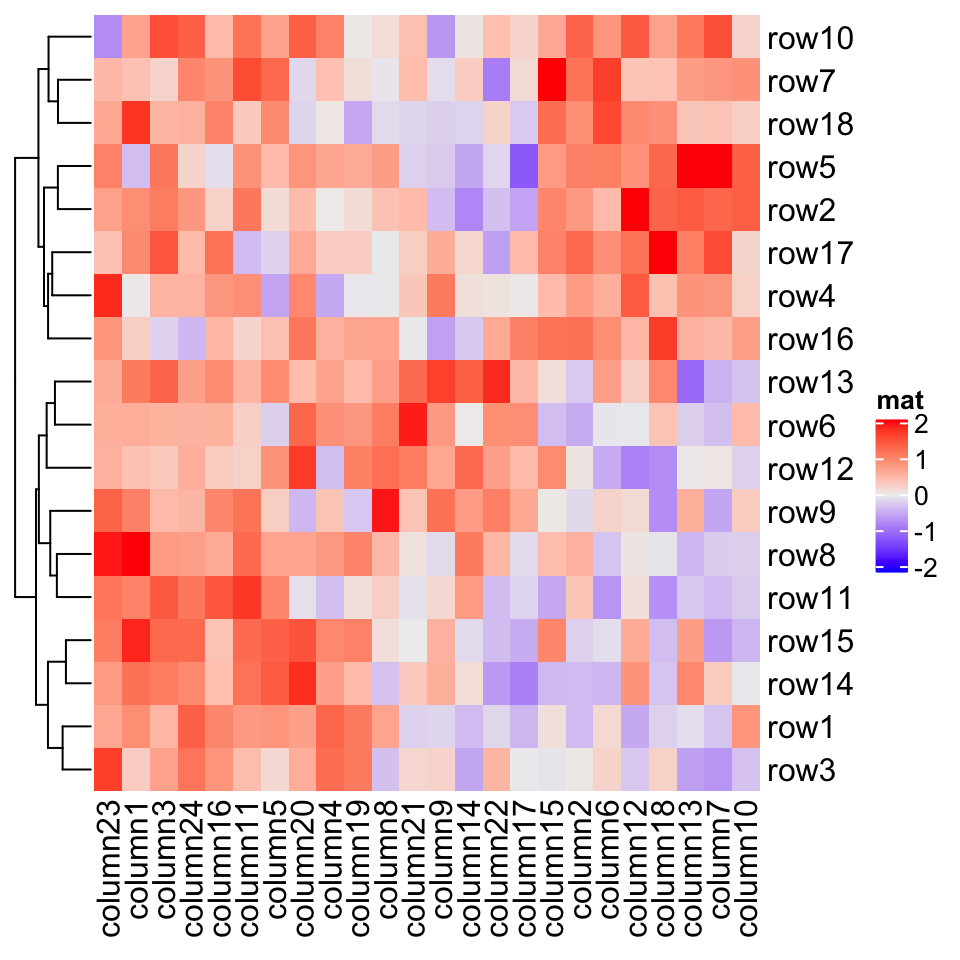
\includegraphics{02-single_heatmap_files/figure-latex/cluster_basic-2} \end{center}

\begin{Shaded}
\begin{Highlighting}[]
\KeywordTok{Heatmap}\NormalTok{(mat, }\DataTypeTok{name =} \StringTok{"mat"}\NormalTok{, }\DataTypeTok{row_dend_side =} \StringTok{"right"}\NormalTok{, }\DataTypeTok{column_dend_side =} \StringTok{"bottom"}\NormalTok{)}
\end{Highlighting}
\end{Shaded}

\begin{center}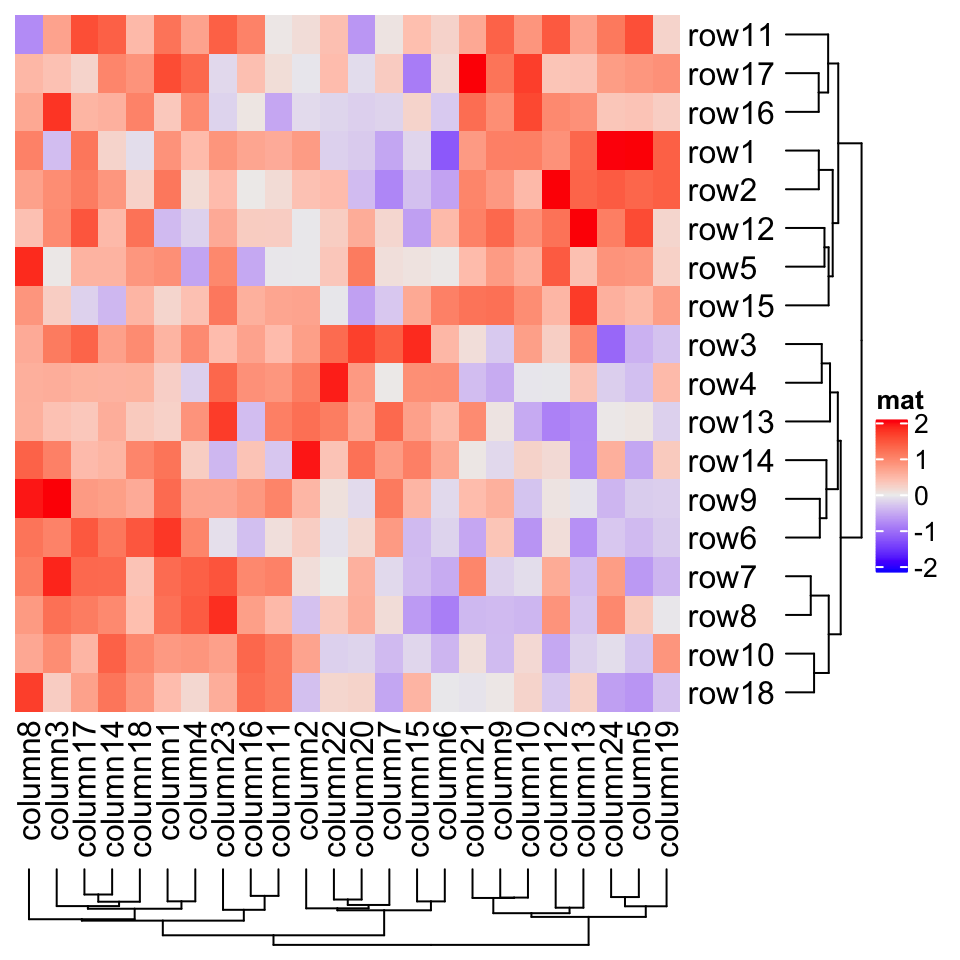
\includegraphics{02-single_heatmap_files/figure-latex/cluster_basic-3} \end{center}

\begin{Shaded}
\begin{Highlighting}[]
\KeywordTok{Heatmap}\NormalTok{(mat, }\DataTypeTok{name =} \StringTok{"mat"}\NormalTok{, }\DataTypeTok{column_dend_height =} \KeywordTok{unit}\NormalTok{(}\DecValTok{4}\NormalTok{, }\StringTok{"cm"}\NormalTok{), }
    \DataTypeTok{row_dend_width =} \KeywordTok{unit}\NormalTok{(}\DecValTok{4}\NormalTok{, }\StringTok{"cm"}\NormalTok{))}
\end{Highlighting}
\end{Shaded}

\begin{center}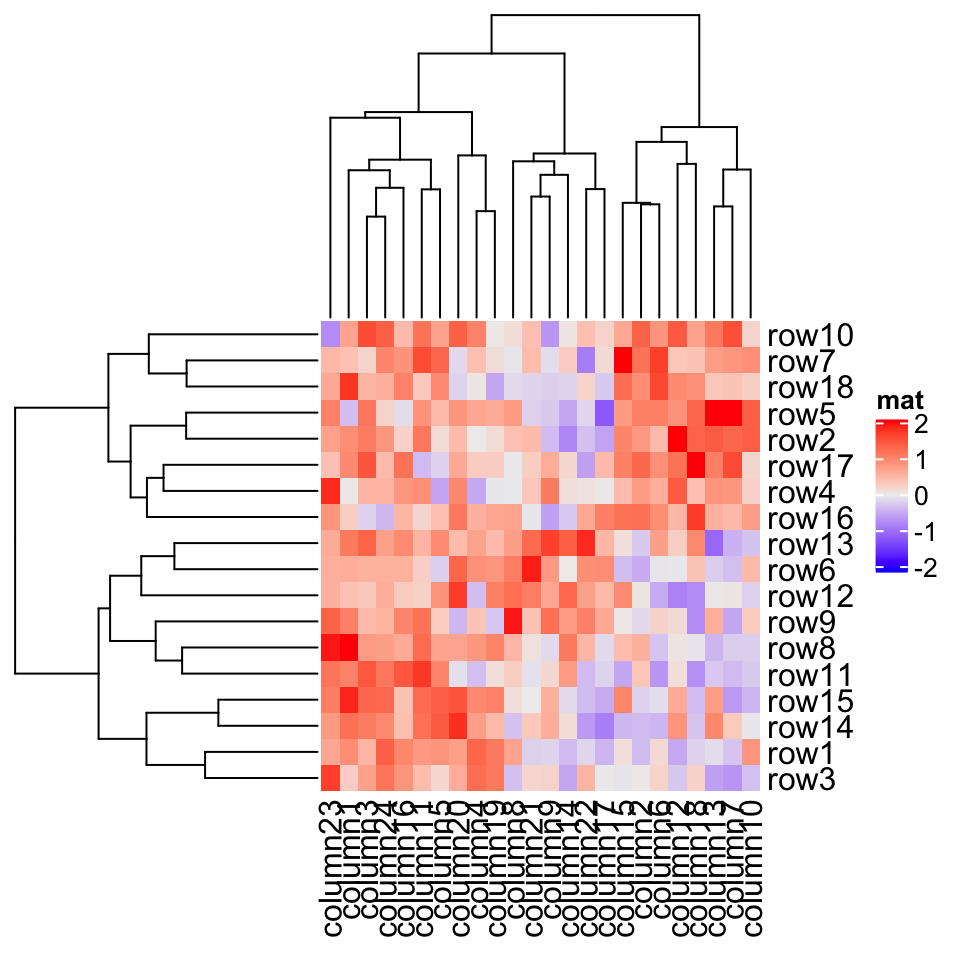
\includegraphics{02-single_heatmap_files/figure-latex/cluster_basic-4} \end{center}

\subsection{Distance methods}\label{distance-methods}

Hierarchical clustering is performed in two steps: calculate the
distance matrix and apply clustering. There are three ways to specify
distance metric for clustering:

\begin{itemize}
\tightlist
\item
  specify distance as a pre-defined option. The valid values are the
  supported methods in \texttt{dist()} function and in
  \texttt{"pearson"}, \texttt{"spearman"} and \texttt{"kendall"}. If
  there is any \texttt{NA} values in the matrix,
  \texttt{ComplexHeatmap::dist2()} is used instead which performs
  pairwise distance calculation by removing \texttt{NA} values. The
  correlation distance is defined as \texttt{1\ -\ cor(x,\ y,\ method)}.
\item
  a self-defined function which calculates distance from a matrix. The
  function should only contain one argument. Please note for clustering
  on columns, the matrix will be transposed automatically.
\item
  a self-defined function which calculates distance from two vectors.
  The function should only contain two arguments.
\end{itemize}

\begin{Shaded}
\begin{Highlighting}[]
\KeywordTok{Heatmap}\NormalTok{(mat, }\DataTypeTok{name =} \StringTok{"mat"}\NormalTok{, }\DataTypeTok{clustering_distance_rows =} \StringTok{"pearson"}\NormalTok{,}
    \DataTypeTok{column_title =} \StringTok{"pre-defined distance method (1 - pearson)"}\NormalTok{)}
\end{Highlighting}
\end{Shaded}

\begin{center}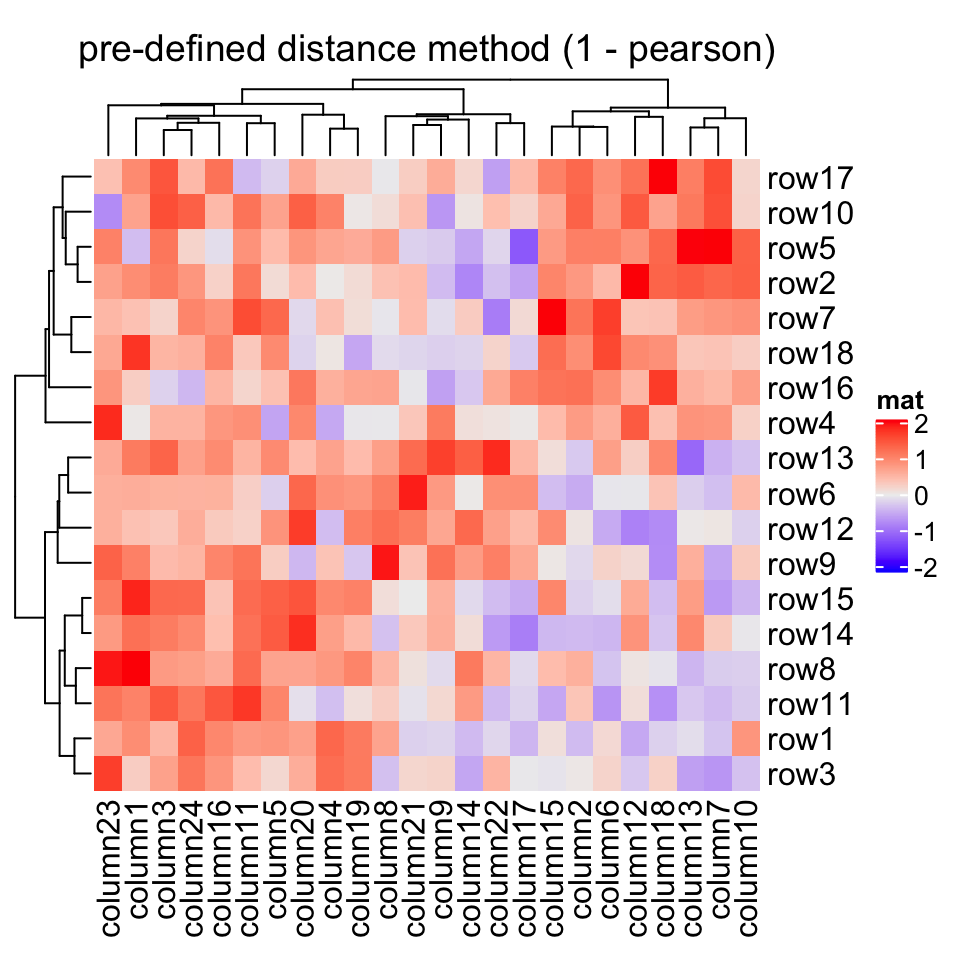
\includegraphics{02-single_heatmap_files/figure-latex/cluster_distance-1} \end{center}

\begin{Shaded}
\begin{Highlighting}[]
\KeywordTok{Heatmap}\NormalTok{(mat, }\DataTypeTok{name =} \StringTok{"mat"}\NormalTok{, }\DataTypeTok{clustering_distance_rows =} \ControlFlowTok{function}\NormalTok{(m) }\KeywordTok{dist}\NormalTok{(m),}
    \DataTypeTok{column_title =} \StringTok{"a function that calculates distance matrix"}\NormalTok{)}
\end{Highlighting}
\end{Shaded}

\begin{center}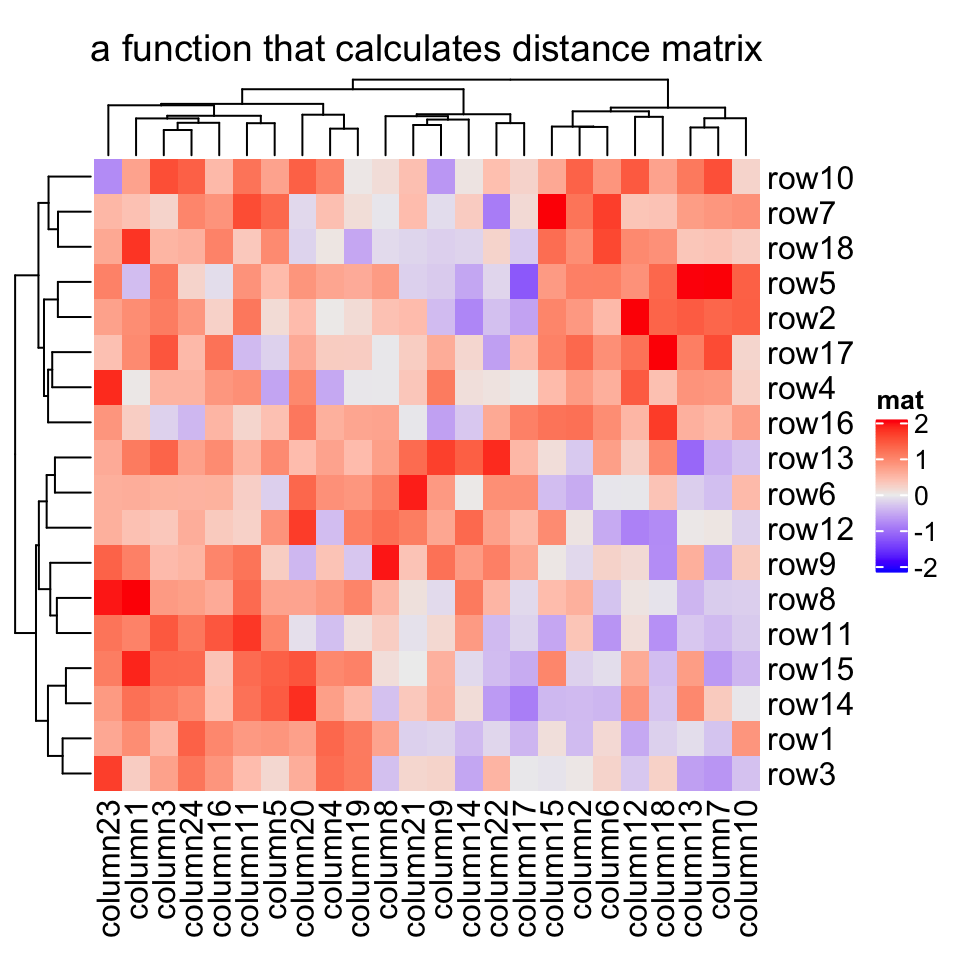
\includegraphics{02-single_heatmap_files/figure-latex/cluster_distance-2} \end{center}

\begin{Shaded}
\begin{Highlighting}[]
\KeywordTok{Heatmap}\NormalTok{(mat, }\DataTypeTok{name =} \StringTok{"mat"}\NormalTok{, }\DataTypeTok{clustering_distance_rows =} \ControlFlowTok{function}\NormalTok{(x, y) }\DecValTok{1} \OperatorTok{-}\StringTok{ }\KeywordTok{cor}\NormalTok{(x, y),}
    \DataTypeTok{column_title =} \StringTok{"a function that calculates pairwise distance"}\NormalTok{)}
\end{Highlighting}
\end{Shaded}

\begin{center}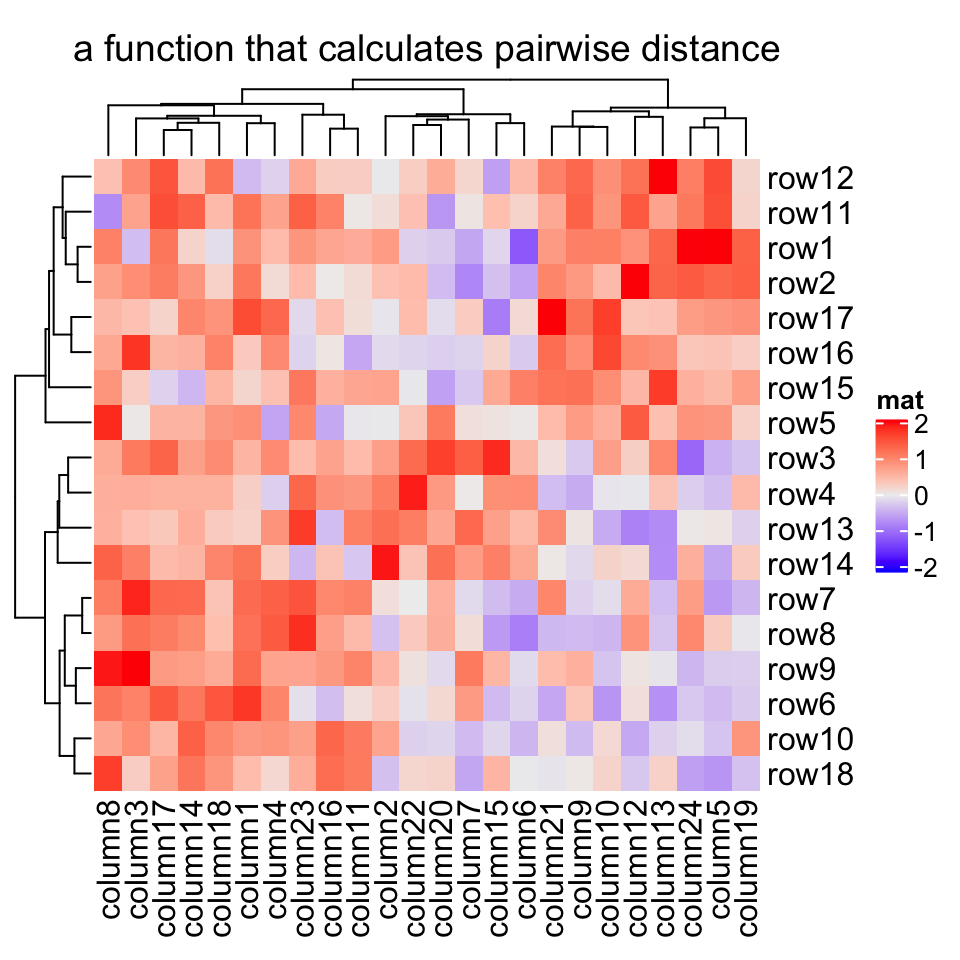
\includegraphics{02-single_heatmap_files/figure-latex/cluster_distance-3} \end{center}

Based on these features, we can apply clustering which is robust to
outliers based on the pairwise distance. Note here we set the color
mapping function because we don't want outliers affect the colors.

\begin{Shaded}
\begin{Highlighting}[]
\NormalTok{mat_with_outliers =}\StringTok{ }\NormalTok{mat}
\ControlFlowTok{for}\NormalTok{(i }\ControlFlowTok{in}  \DecValTok{1}\OperatorTok{:}\DecValTok{10}\NormalTok{) mat_with_outliers[i, i] =}\StringTok{ }\DecValTok{1000}
\NormalTok{robust_dist =}\StringTok{ }\ControlFlowTok{function}\NormalTok{(x, y) \{}
\NormalTok{    qx =}\StringTok{ }\KeywordTok{quantile}\NormalTok{(x, }\KeywordTok{c}\NormalTok{(}\FloatTok{0.1}\NormalTok{, }\FloatTok{0.9}\NormalTok{))}
\NormalTok{    qy =}\StringTok{ }\KeywordTok{quantile}\NormalTok{(y, }\KeywordTok{c}\NormalTok{(}\FloatTok{0.1}\NormalTok{, }\FloatTok{0.9}\NormalTok{))}
\NormalTok{    l =}\StringTok{ }\NormalTok{x }\OperatorTok{>}\StringTok{ }\NormalTok{qx[}\DecValTok{1}\NormalTok{] }\OperatorTok{&}\StringTok{ }\NormalTok{x }\OperatorTok{<}\StringTok{ }\NormalTok{qx[}\DecValTok{2}\NormalTok{] }\OperatorTok{&}\StringTok{ }\NormalTok{y }\OperatorTok{>}\StringTok{ }\NormalTok{qy[}\DecValTok{1}\NormalTok{] }\OperatorTok{&}\StringTok{ }\NormalTok{y }\OperatorTok{<}\StringTok{ }\NormalTok{qy[}\DecValTok{2}\NormalTok{]}
\NormalTok{    x =}\StringTok{ }\NormalTok{x[l]}
\NormalTok{    y =}\StringTok{ }\NormalTok{y[l]}
    \KeywordTok{sqrt}\NormalTok{(}\KeywordTok{sum}\NormalTok{((x }\OperatorTok{-}\StringTok{ }\NormalTok{y)}\OperatorTok{^}\DecValTok{2}\NormalTok{))}
\NormalTok{\}}
\end{Highlighting}
\end{Shaded}

and we compare the two heatmaps with or without the robust distance
method:

\begin{Shaded}
\begin{Highlighting}[]
\KeywordTok{Heatmap}\NormalTok{(mat_with_outliers, }\DataTypeTok{name =} \StringTok{"mat"}\NormalTok{, }
    \DataTypeTok{col =} \KeywordTok{colorRamp2}\NormalTok{(}\KeywordTok{c}\NormalTok{(}\OperatorTok{-}\DecValTok{2}\NormalTok{, }\DecValTok{0}\NormalTok{, }\DecValTok{2}\NormalTok{), }\KeywordTok{c}\NormalTok{(}\StringTok{"green"}\NormalTok{, }\StringTok{"white"}\NormalTok{, }\StringTok{"red"}\NormalTok{)),}
    \DataTypeTok{column_title =} \StringTok{"dist"}\NormalTok{)}
\KeywordTok{Heatmap}\NormalTok{(mat_with_outliers, }\DataTypeTok{name =} \StringTok{"mat"}\NormalTok{, }
    \DataTypeTok{col =} \KeywordTok{colorRamp2}\NormalTok{(}\KeywordTok{c}\NormalTok{(}\OperatorTok{-}\DecValTok{2}\NormalTok{, }\DecValTok{0}\NormalTok{, }\DecValTok{2}\NormalTok{), }\KeywordTok{c}\NormalTok{(}\StringTok{"green"}\NormalTok{, }\StringTok{"white"}\NormalTok{, }\StringTok{"red"}\NormalTok{)),}
    \DataTypeTok{clustering_distance_rows =}\NormalTok{ robust_dist,}
    \DataTypeTok{clustering_distance_columns =}\NormalTok{ robust_dist,}
    \DataTypeTok{column_title =} \StringTok{"robust_dist"}\NormalTok{)}
\end{Highlighting}
\end{Shaded}

\begin{center}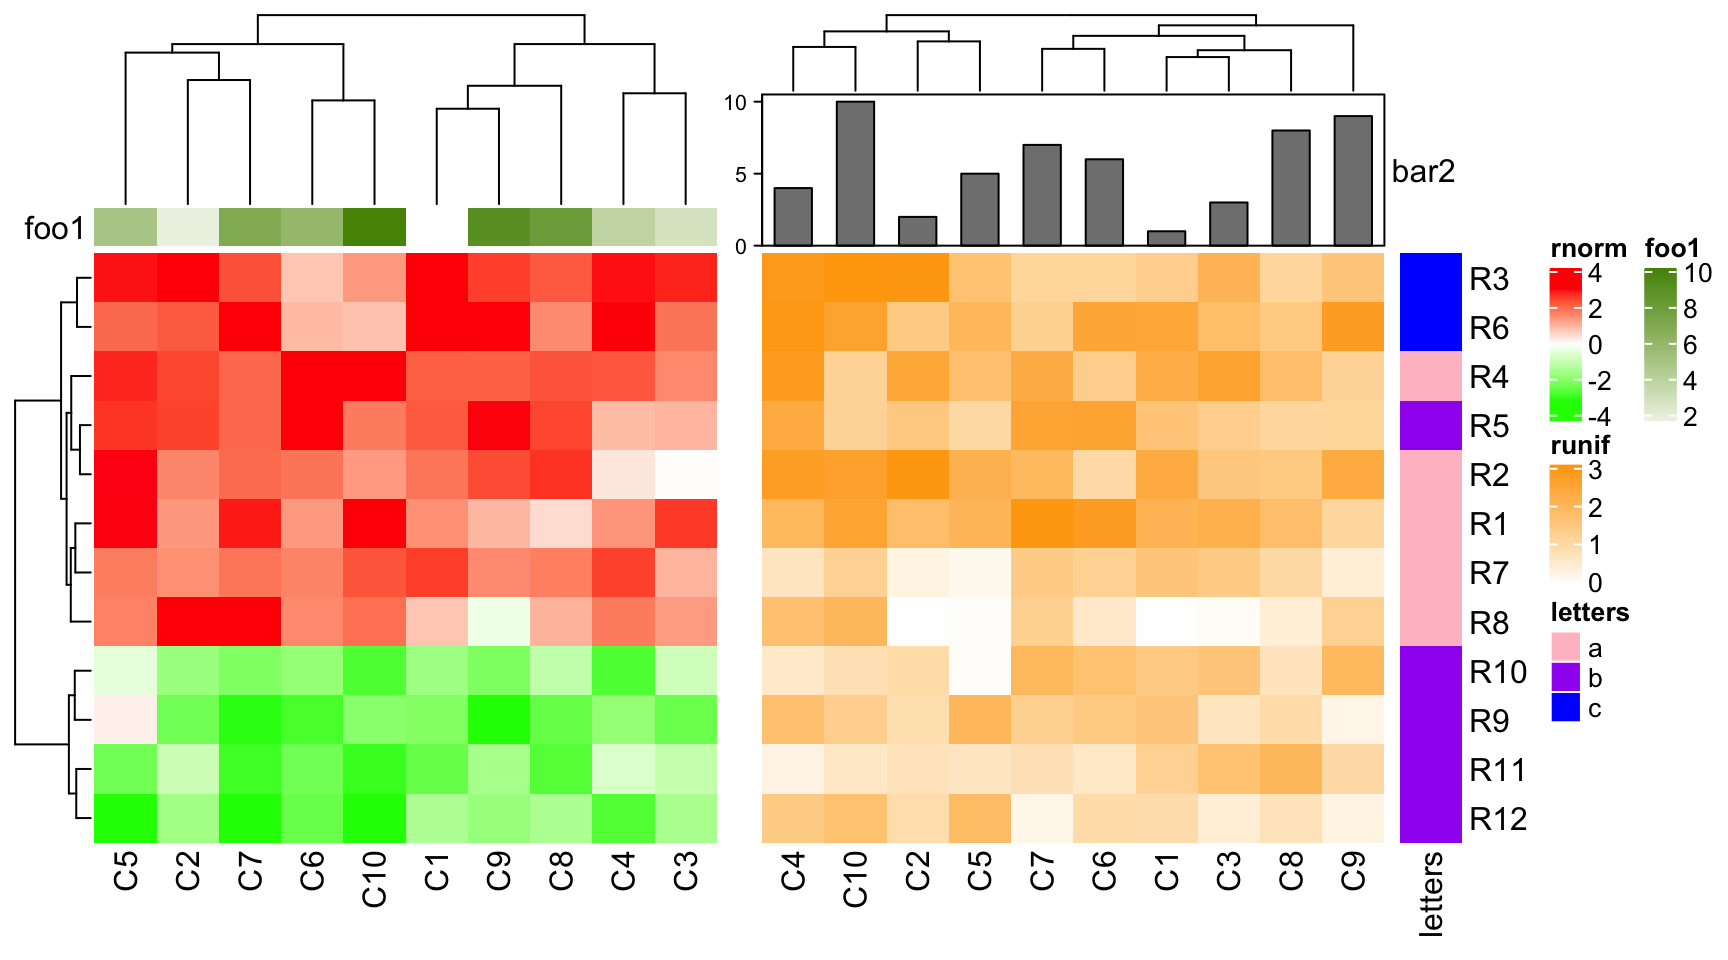
\includegraphics{02-single_heatmap_files/figure-latex/unnamed-chunk-14-1} \end{center}

If there are proper distance methods (like methods in
\href{https://cran.r-project.org/web/packages/stringdist/}{\textbf{stringdist}
package}, you can also cluster a character matrix. \texttt{cell\_fun}
argument will be introduced in Section \ref{customize-the-heatmap-body}.

\begin{Shaded}
\begin{Highlighting}[]
\NormalTok{mat_letters =}\StringTok{ }\KeywordTok{matrix}\NormalTok{(}\KeywordTok{sample}\NormalTok{(letters[}\DecValTok{1}\OperatorTok{:}\DecValTok{4}\NormalTok{], }\DecValTok{100}\NormalTok{, }\DataTypeTok{replace =} \OtherTok{TRUE}\NormalTok{), }\DecValTok{10}\NormalTok{)}
\CommentTok{# distance in the ASCII table}
\NormalTok{dist_letters =}\StringTok{ }\ControlFlowTok{function}\NormalTok{(x, y) \{}
\NormalTok{    x =}\StringTok{ }\KeywordTok{strtoi}\NormalTok{(}\KeywordTok{charToRaw}\NormalTok{(}\KeywordTok{paste}\NormalTok{(x, }\DataTypeTok{collapse =} \StringTok{""}\NormalTok{)), }\DataTypeTok{base =} \DecValTok{16}\NormalTok{)}
\NormalTok{    y =}\StringTok{ }\KeywordTok{strtoi}\NormalTok{(}\KeywordTok{charToRaw}\NormalTok{(}\KeywordTok{paste}\NormalTok{(y, }\DataTypeTok{collapse =} \StringTok{""}\NormalTok{)), }\DataTypeTok{base =} \DecValTok{16}\NormalTok{)}
    \KeywordTok{sqrt}\NormalTok{(}\KeywordTok{sum}\NormalTok{((x }\OperatorTok{-}\StringTok{ }\NormalTok{y)}\OperatorTok{^}\DecValTok{2}\NormalTok{))}
\NormalTok{\}}
\KeywordTok{Heatmap}\NormalTok{(mat_letters, }\DataTypeTok{name =} \StringTok{"letters"}\NormalTok{, }\DataTypeTok{col =} \KeywordTok{structure}\NormalTok{(}\DecValTok{2}\OperatorTok{:}\DecValTok{5}\NormalTok{, }\DataTypeTok{names =}\NormalTok{ letters[}\DecValTok{1}\OperatorTok{:}\DecValTok{4}\NormalTok{]),}
    \DataTypeTok{clustering_distance_rows =}\NormalTok{ dist_letters, }\DataTypeTok{clustering_distance_columns =}\NormalTok{ dist_letters,}
    \DataTypeTok{cell_fun =} \ControlFlowTok{function}\NormalTok{(j, i, x, y, w, h, col) \{ }\CommentTok{# add text to each grid}
        \KeywordTok{grid.text}\NormalTok{(mat_letters[i, j], x, y)}
\NormalTok{    \})}
\end{Highlighting}
\end{Shaded}

\begin{center}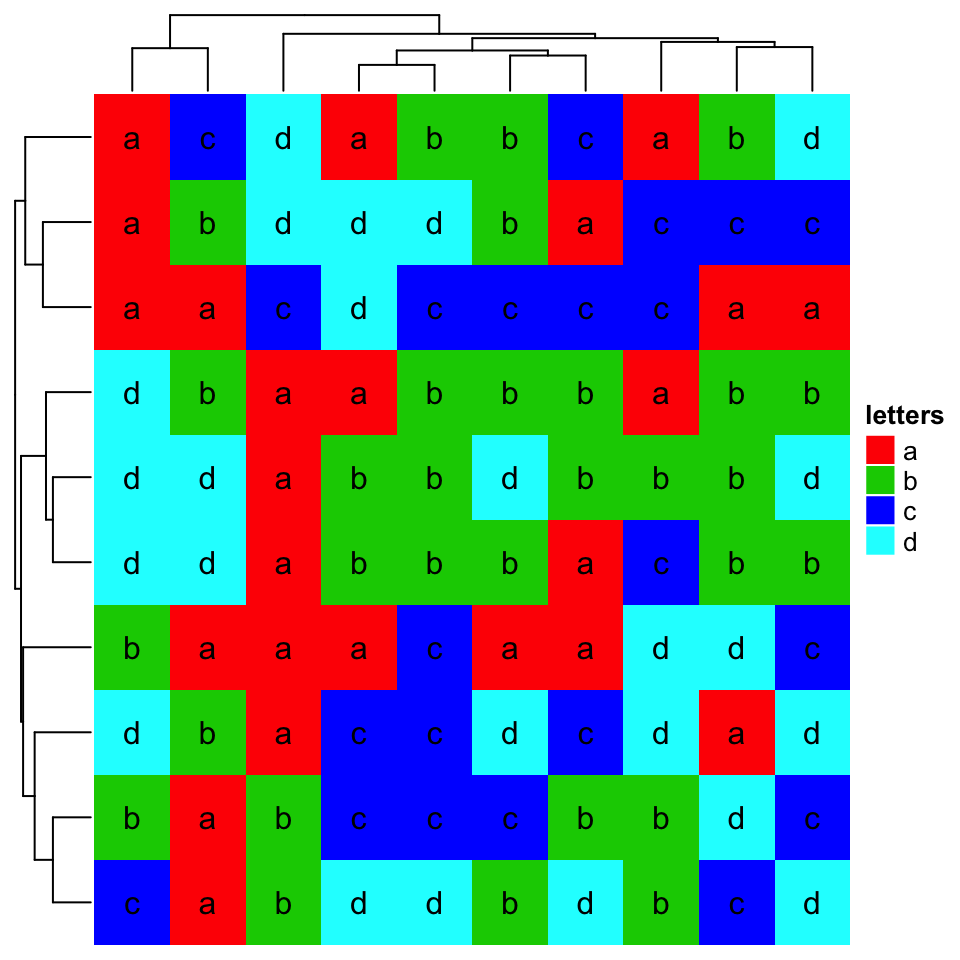
\includegraphics{02-single_heatmap_files/figure-latex/cluster_character_matrix-1} \end{center}

\subsection{Clustering methods}\label{clustering-methods}

Method to perform hierarchical clustering can be specified by
\texttt{clustering\_method\_rows} and
\texttt{clustering\_method\_columns}. Possible methods are those
supported in \texttt{hclust()} function.

\begin{Shaded}
\begin{Highlighting}[]
\KeywordTok{Heatmap}\NormalTok{(mat, }\DataTypeTok{name =} \StringTok{"mat"}\NormalTok{, }\DataTypeTok{clustering_method_rows =} \StringTok{"single"}\NormalTok{)}
\end{Highlighting}
\end{Shaded}

\begin{center}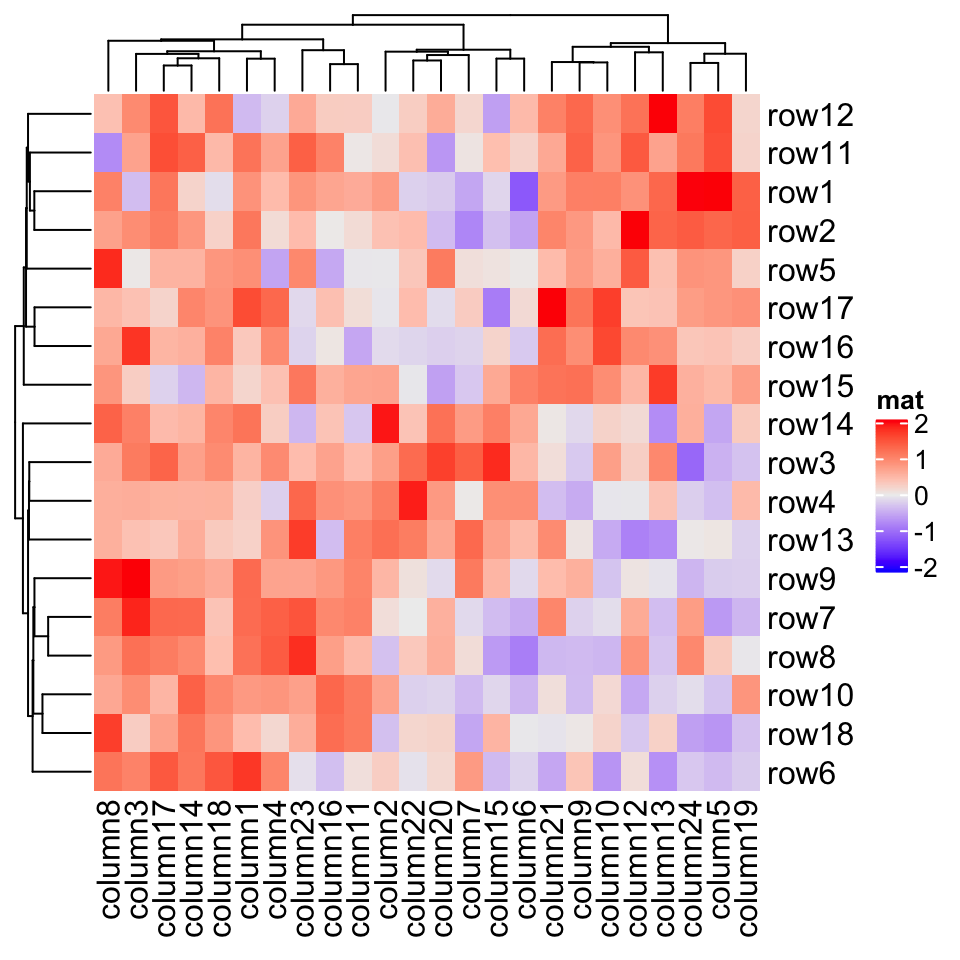
\includegraphics{02-single_heatmap_files/figure-latex/cluster_method-1} \end{center}

If you already have clustering objects or a function which directly
returns a clustering object, you can ignore the distance settings and
set \texttt{cluster\_rows} or \texttt{cluster\_columns} to the
clustering objects or clustering functions. If it is a clustering
function, the only argument should be the matrix and it should return a
\texttt{hclust} or \texttt{dendrogram} object or a object that can be
coerced to the two classes.

In following example, we perform clustering with methods from
\textbf{cluster} package either by a pre-calculated clustering object or
a clustering function:

\begin{Shaded}
\begin{Highlighting}[]
\KeywordTok{library}\NormalTok{(cluster)}
\KeywordTok{Heatmap}\NormalTok{(mat, }\DataTypeTok{name =} \StringTok{"mat"}\NormalTok{, }\DataTypeTok{cluster_rows =} \KeywordTok{as.dendrogram}\NormalTok{(}\KeywordTok{diana}\NormalTok{(mat)),}
   \DataTypeTok{cluster_columns =} \KeywordTok{as.dendrogram}\NormalTok{(}\KeywordTok{agnes}\NormalTok{(}\KeywordTok{t}\NormalTok{(mat))), }\DataTypeTok{column_title =} \StringTok{"clustering objects"}\NormalTok{)}
\end{Highlighting}
\end{Shaded}

\begin{center}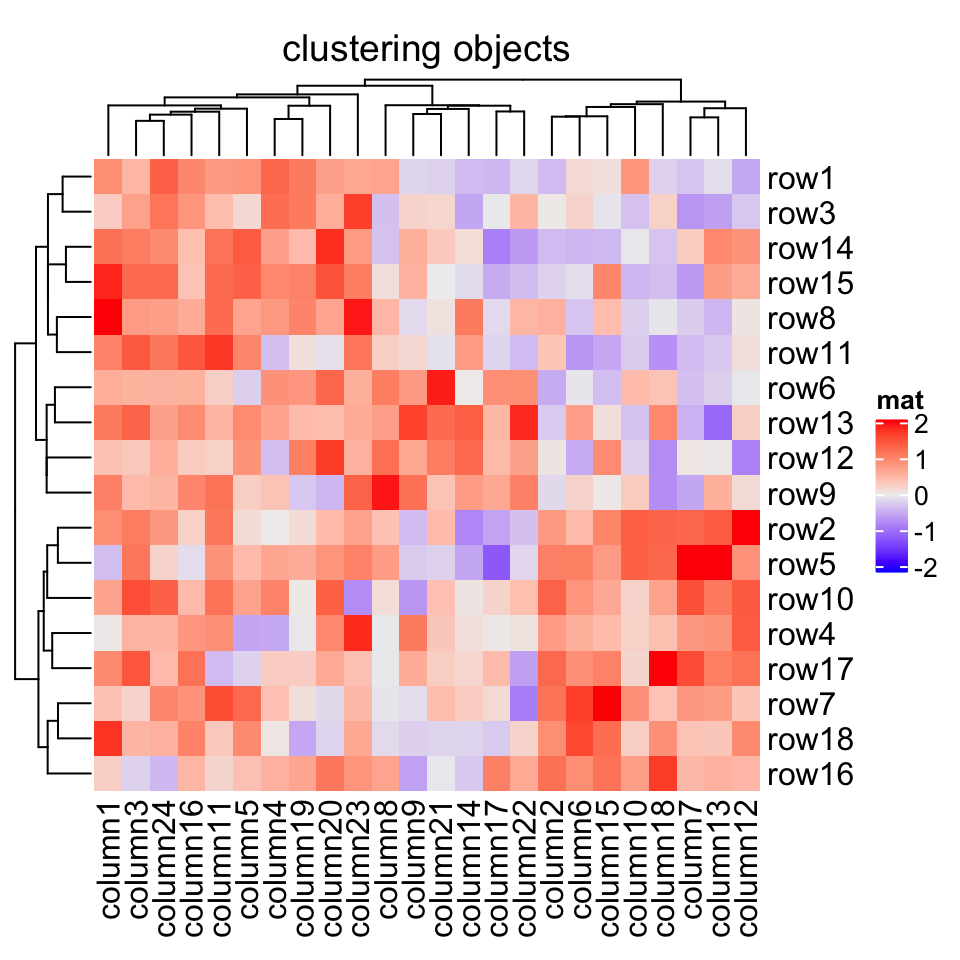
\includegraphics{02-single_heatmap_files/figure-latex/cluster_object-1} \end{center}

\begin{Shaded}
\begin{Highlighting}[]
\KeywordTok{Heatmap}\NormalTok{(mat, }\DataTypeTok{name =} \StringTok{"mat"}\NormalTok{, }\DataTypeTok{cluster_rows =}\NormalTok{ diana,}
   \DataTypeTok{cluster_columns =}\NormalTok{ agnes, }\DataTypeTok{column_title =} \StringTok{"clustering functions"}\NormalTok{)}
\end{Highlighting}
\end{Shaded}

\begin{center}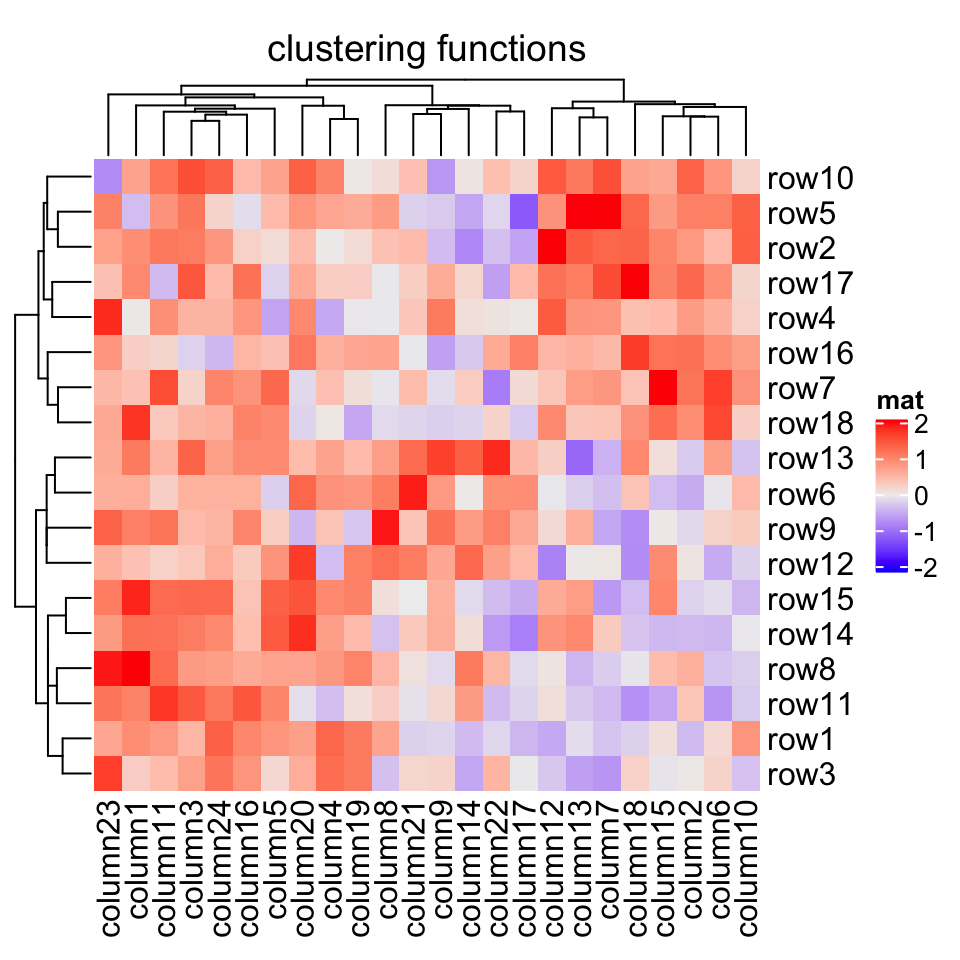
\includegraphics{02-single_heatmap_files/figure-latex/cluster_object-2} \end{center}

The last command is as same as :

\begin{Shaded}
\begin{Highlighting}[]
\CommentTok{# code only for demonstration}
\KeywordTok{Heatmap}\NormalTok{(mat, }\DataTypeTok{name =} \StringTok{"mat"}\NormalTok{, }\DataTypeTok{cluster_rows =} \ControlFlowTok{function}\NormalTok{(m) }\KeywordTok{as.dendrogram}\NormalTok{(}\KeywordTok{diana}\NormalTok{(m)),}
    \DataTypeTok{cluster_columns =} \ControlFlowTok{function}\NormalTok{(m) }\KeywordTok{as.dendrogram}\NormalTok{(}\KeywordTok{agnes}\NormalTok{(m)), }\DataTypeTok{column_title =} \StringTok{"clutering functions"}\NormalTok{)}
\end{Highlighting}
\end{Shaded}

Please note, when \texttt{cluster\_rows} is set as a function, the
argument \texttt{m} is the input \texttt{mat} itself, while for
\texttt{cluster\_columns}, \texttt{m} is the transpose of \texttt{mat}.

\texttt{fastcluster::hclust} implements a faster version of
\texttt{hclust()}. We can set it to \texttt{cluster\_rows} and
\texttt{cluster\_columns} to use the faster version of
\texttt{hclust()}.

\begin{Shaded}
\begin{Highlighting}[]
\CommentTok{# code only for demonstration}
\KeywordTok{Heatmap}\NormalTok{(mat, }\DataTypeTok{name =} \StringTok{"mat"}\NormalTok{, }\DataTypeTok{cluster_rows =}\NormalTok{ fastcluster}\OperatorTok{::}\NormalTok{hclust, }
    \DataTypeTok{cluster_columns =}\NormalTok{ fastcluster}\OperatorTok{::}\NormalTok{hclust)}
\end{Highlighting}
\end{Shaded}

To make it more convinient to use the faster version of
\texttt{hclust()} (assuming you have many heatmaps to construct), it can
be set as a global option. The usage of \texttt{ht\_opt} is introduced
in Section \ref{change-graphic-parameters-simultaneously}.

\begin{Shaded}
\begin{Highlighting}[]
\CommentTok{# code not run when building the vignette}
\NormalTok{ht_opt}\OperatorTok{$}\NormalTok{fast_hclust =}\StringTok{ }\OtherTok{TRUE}
\CommentTok{# now fastcluster::hclust is used in all heatmaps}
\end{Highlighting}
\end{Shaded}

\subsection{Render dendrograms}\label{render-dendrograms}

If you want to render the dendrogram, normally you need to generate a
\texttt{dendrogram} object and render it in the first place, then send
it to the \texttt{cluster\_rows} or \texttt{cluster\_columns} argument.

You can render your \texttt{dendrogram} object by the
\textbf{dendextend} package to make a more customized visualization of
the dendrogram. Note \textbf{ComplexHeatmap} only allows rendering on
the dendrogram edges.

\begin{Shaded}
\begin{Highlighting}[]
\KeywordTok{library}\NormalTok{(dendextend)}
\NormalTok{row_dend =}\StringTok{ }\KeywordTok{as.dendrogram}\NormalTok{(}\KeywordTok{hclust}\NormalTok{(}\KeywordTok{dist}\NormalTok{(mat)))}
\NormalTok{row_dend =}\StringTok{ }\KeywordTok{color_branches}\NormalTok{(row_dend, }\DataTypeTok{k =} \DecValTok{2}\NormalTok{) }\CommentTok{# `color_branches()` returns a dendrogram object}
\KeywordTok{Heatmap}\NormalTok{(mat, }\DataTypeTok{name =} \StringTok{"mat"}\NormalTok{, }\DataTypeTok{cluster_rows =}\NormalTok{ row_dend)}
\end{Highlighting}
\end{Shaded}

\begin{center}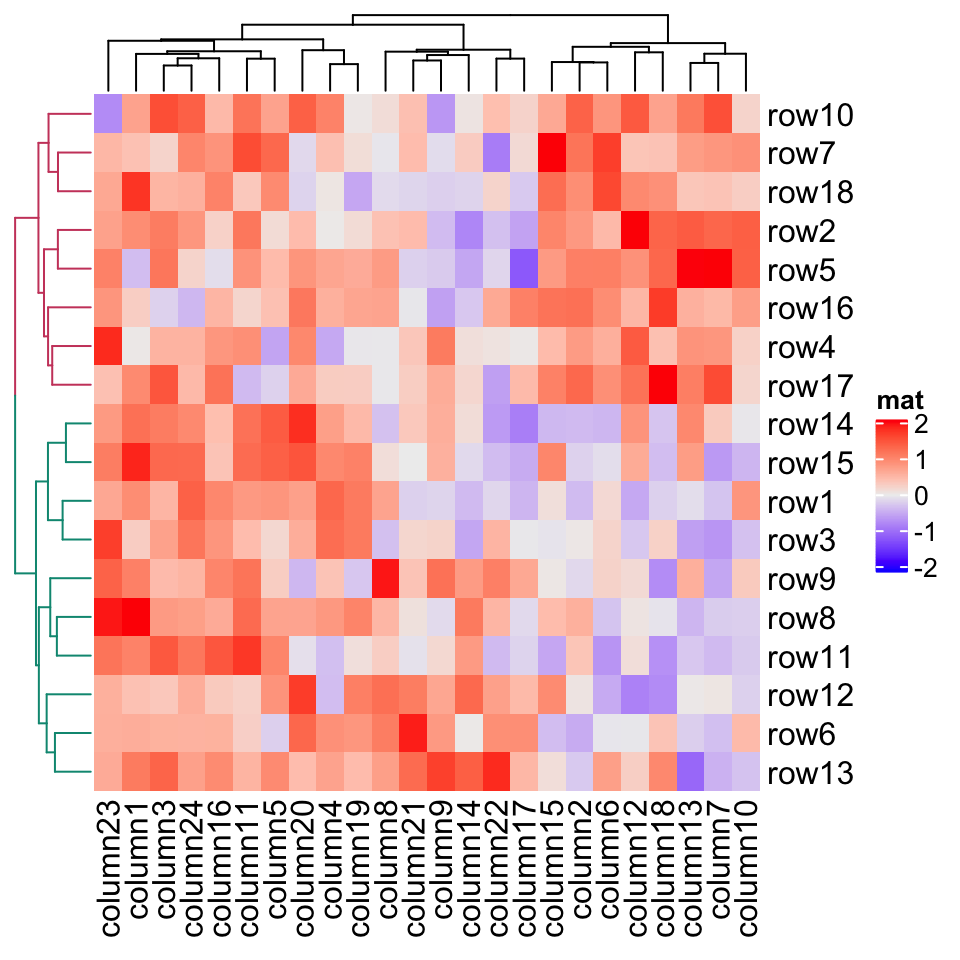
\includegraphics{02-single_heatmap_files/figure-latex/cluster_dendextend-1} \end{center}

\subsection{Reorder dendrograms}\label{reorder-dendrograms}

In the \texttt{Heatmap()} function, dendrograms are reordered to make
features with larger difference more separated from each others (please
refer to the documentation of \texttt{reorder.dendrogram()}). Here the
difference (or it is called the weight) is measured by the row means if
it is a row dendrogram or by the column means if it is a column
dendrogram. \texttt{row\_dend\_reorder} and
\texttt{column\_dend\_reorder} control whether to apply dendrogram
reordering If they are set to \texttt{TRUE} or \texttt{FALSE}, ot they
control the weight for the reordering if they are set to numeric vectors
(send to the \texttt{wts} argument of \texttt{reorder.dendrogram()}).
The reordering can be turned off by setting e.g.
\texttt{row\_dend\_reorder\ =\ FALSE}.

There are many other methods for reordering dendrograms, e.g.~the
\textbf{dendsort} package. Basically, all these methods still return a
dendrogram that has been reordered, thus, we can firstly generate the
row or column dendrogram based on the data matrix, reorder it by some
method, and assign it back to \texttt{cluster\_rows} or
\texttt{cluster\_columns}.

Compare following three heatmaps:

\begin{Shaded}
\begin{Highlighting}[]
\KeywordTok{Heatmap}\NormalTok{(mat, }\DataTypeTok{name =} \StringTok{"mat"}\NormalTok{, }\DataTypeTok{row_dend_reorder =} \OtherTok{FALSE}\NormalTok{, }\DataTypeTok{column_title =} \StringTok{"no reordering"}\NormalTok{)}
\KeywordTok{Heatmap}\NormalTok{(mat, }\DataTypeTok{name =} \StringTok{"mat"}\NormalTok{, }\DataTypeTok{row_dend_reorder =} \OtherTok{TRUE}\NormalTok{, }\DataTypeTok{column_title =} \StringTok{"applied reordering"}\NormalTok{)}

\KeywordTok{library}\NormalTok{(dendsort)}
\NormalTok{dend =}\StringTok{ }\KeywordTok{dendsort}\NormalTok{(}\KeywordTok{as.dendrogram}\NormalTok{(}\KeywordTok{hclust}\NormalTok{(}\KeywordTok{dist}\NormalTok{(mat))))}
\KeywordTok{Heatmap}\NormalTok{(mat, }\DataTypeTok{name =} \StringTok{"mat"}\NormalTok{, }\DataTypeTok{cluster_rows =}\NormalTok{ dend, }\DataTypeTok{row_dend_reorder =} \OtherTok{FALSE}\NormalTok{, }
    \DataTypeTok{column_title =} \StringTok{"reordering by dendsort"}\NormalTok{)}
\end{Highlighting}
\end{Shaded}

\begin{center}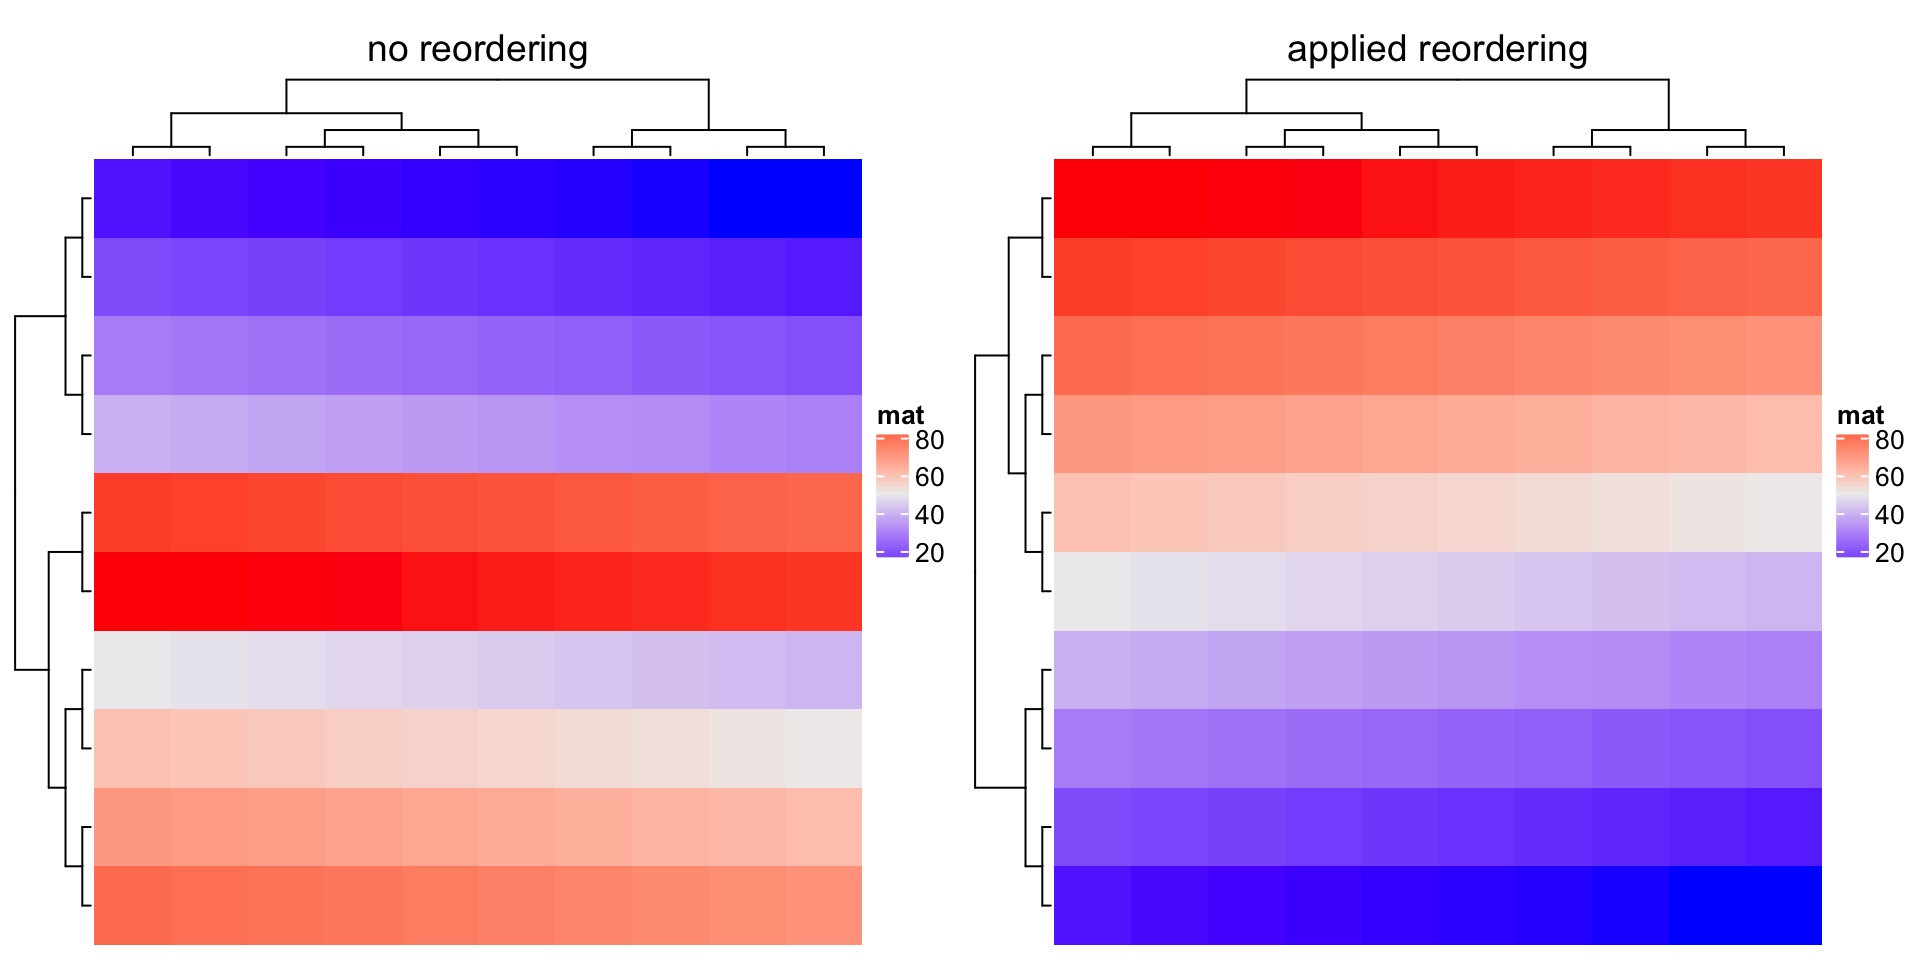
\includegraphics{02-single_heatmap_files/figure-latex/cluster_dendsort-1} \end{center}

\section{Row and column orders}\label{row-and_column_orders}

Clustering is used to adjust row orders and column orders of the
heatmap, but you can still set the order manually by \texttt{row\_order}
and \texttt{column\_order}. If e.g. \texttt{row\_order} is set, row
clustering is turned off.

\begin{Shaded}
\begin{Highlighting}[]
\KeywordTok{Heatmap}\NormalTok{(mat, }\DataTypeTok{name =} \StringTok{"mat"}\NormalTok{, }\DataTypeTok{row_order =} \KeywordTok{order}\NormalTok{(}\KeywordTok{rownames}\NormalTok{(mat)), }
    \DataTypeTok{column_order =} \KeywordTok{order}\NormalTok{(}\KeywordTok{colnames}\NormalTok{(mat)))}
\end{Highlighting}
\end{Shaded}

\begin{center}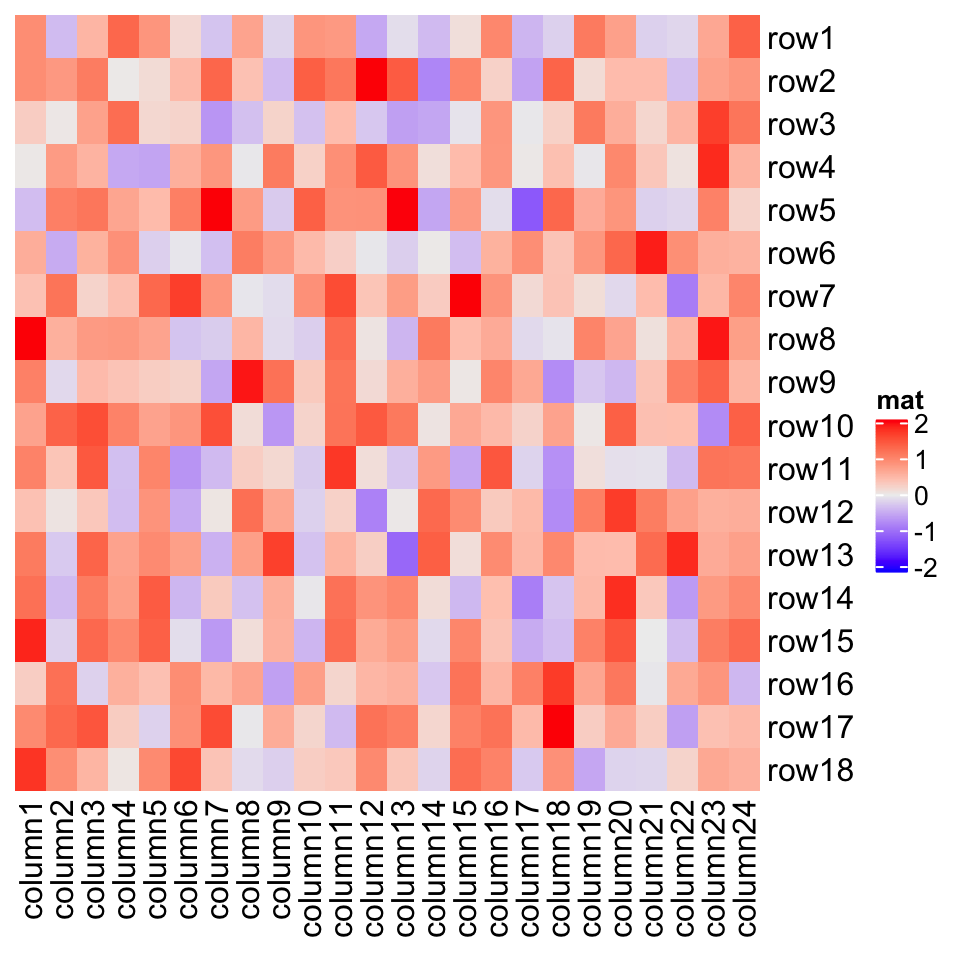
\includegraphics{02-single_heatmap_files/figure-latex/manual_order-1} \end{center}

Note \texttt{row\_dend\_reorder} and \texttt{row\_order} are two
different things. \texttt{row\_dend\_reorder} is applied on the
dendrogram. For any node in the dendrogram, rotating its two branches
actually gives an identical dendrogram, thus, reordering the dendrogram
by automatically rotating sub-dendrogram at every node can help to
separate elements further from each other which show more difference. As
a comparison, \texttt{row\_order} is simply applied on the matrix and
normally dendrograms should be turned off.

\section{Seriation}\label{heatmap-seriation}

Seriation is an interesting technique for ordering the matrix (see this
interesting post:
\url{http://nicolas.kruchten.com/content/2018/02/seriation/}). The
powerful
\href{https://cran.r-project.org/web/packages/seriation/index.html}{\textbf{seriation}
package} implements quite a lot of methods for seriation. Since it is
easy to extract row orders and column ordes from the object returned by
the core function \texttt{seriate()} from \textbf{seriation} package.
They can be directly assigned to \texttt{row\_order} and
\texttt{column\_order} to make the heatmap.

The first example demonstrates to directly apply \texttt{seriate()} on
the matrix. Since the \texttt{"BEA\_TSP"} method only allows a
non-negative matrix, we modify the matrix to \texttt{max(mat)\ -\ mat}.

\begin{Shaded}
\begin{Highlighting}[]
\KeywordTok{library}\NormalTok{(seriation)}
\NormalTok{o =}\StringTok{ }\KeywordTok{seriate}\NormalTok{(}\KeywordTok{max}\NormalTok{(mat) }\OperatorTok{-}\StringTok{ }\NormalTok{mat, }\DataTypeTok{method =} \StringTok{"BEA_TSP"}\NormalTok{)}
\KeywordTok{Heatmap}\NormalTok{(}\KeywordTok{max}\NormalTok{(mat) }\OperatorTok{-}\StringTok{ }\NormalTok{mat, }\DataTypeTok{name =} \StringTok{"mat"}\NormalTok{, }
    \DataTypeTok{row_order =} \KeywordTok{get_order}\NormalTok{(o, }\DecValTok{1}\NormalTok{), }\DataTypeTok{column_order =} \KeywordTok{get_order}\NormalTok{(o, }\DecValTok{2}\NormalTok{))}
\end{Highlighting}
\end{Shaded}

\begin{center}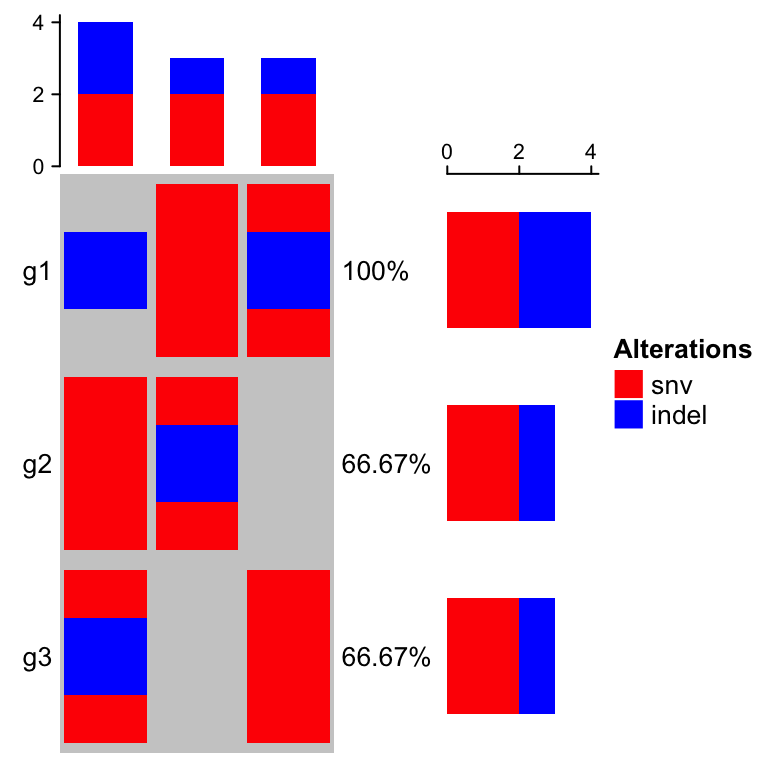
\includegraphics{02-single_heatmap_files/figure-latex/unnamed-chunk-19-1} \end{center}

Or apply \texttt{seriate()} to the distance matrix. Now the order for
rows and columns needs to be calcualted separatedly (because the
distance matrix needs to be calculated separatedly).

\begin{Shaded}
\begin{Highlighting}[]
\NormalTok{o1 =}\StringTok{ }\KeywordTok{seriate}\NormalTok{(}\KeywordTok{dist}\NormalTok{(mat), }\DataTypeTok{method =} \StringTok{"TSP"}\NormalTok{)}
\NormalTok{o2 =}\StringTok{ }\KeywordTok{seriate}\NormalTok{(}\KeywordTok{dist}\NormalTok{(}\KeywordTok{t}\NormalTok{(mat)), }\DataTypeTok{method =} \StringTok{"TSP"}\NormalTok{)}
\KeywordTok{Heatmap}\NormalTok{(mat, }\DataTypeTok{name =} \StringTok{"mat"}\NormalTok{, }\DataTypeTok{row_order =} \KeywordTok{get_order}\NormalTok{(o1), }\DataTypeTok{column_order =} \KeywordTok{get_order}\NormalTok{(o2))}
\end{Highlighting}
\end{Shaded}

\begin{center}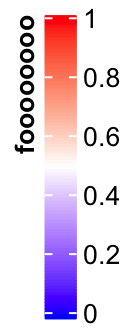
\includegraphics{02-single_heatmap_files/figure-latex/unnamed-chunk-20-1} \end{center}

Some seriation methods also contain the hierarchical clustering
information. Let's try:

\begin{Shaded}
\begin{Highlighting}[]
\NormalTok{o1 =}\StringTok{ }\KeywordTok{seriate}\NormalTok{(}\KeywordTok{dist}\NormalTok{(mat), }\DataTypeTok{method =} \StringTok{"GW"}\NormalTok{)}
\NormalTok{o2 =}\StringTok{ }\KeywordTok{seriate}\NormalTok{(}\KeywordTok{dist}\NormalTok{(}\KeywordTok{t}\NormalTok{(mat)), }\DataTypeTok{method =} \StringTok{"GW"}\NormalTok{)}
\end{Highlighting}
\end{Shaded}

\texttt{o1} and \texttt{o2} are actually mainly composed of
\texttt{hclust} objects:

\begin{Shaded}
\begin{Highlighting}[]
\KeywordTok{class}\NormalTok{(o1[[}\DecValTok{1}\NormalTok{]])}
\end{Highlighting}
\end{Shaded}

\begin{verbatim}
## [1] "ser_permutation_vector" "hclust"
\end{verbatim}

And the orders are the same by using \texttt{hclust\$order} or
\texttt{get\_order()}.

\begin{Shaded}
\begin{Highlighting}[]
\NormalTok{o1[[}\DecValTok{1}\NormalTok{]]}\OperatorTok{$}\NormalTok{order}
\end{Highlighting}
\end{Shaded}

\begin{verbatim}
##  [1]  1  2 11 12  5 15 16 17  7  8  6  9 10 18 13  4  3 14
\end{verbatim}

\begin{Shaded}
\begin{Highlighting}[]
\CommentTok{# should be the same as the previous one}
\KeywordTok{get_order}\NormalTok{(o1)}
\end{Highlighting}
\end{Shaded}

\begin{verbatim}
##  [1]  1  2 11 12  5 15 16 17  7  8  6  9 10 18 13  4  3 14
\end{verbatim}

And we can add the dendrograms to the heatmap (note here we turned off
the default reordering because we exactly want the dendrogram order
returned from seriation).

\begin{Shaded}
\begin{Highlighting}[]
\KeywordTok{Heatmap}\NormalTok{(mat, }\DataTypeTok{cluster_rows =} \KeywordTok{as.dendrogram}\NormalTok{(o1[[}\DecValTok{1}\NormalTok{]]), }\DataTypeTok{row_dend_reorder =} \OtherTok{FALSE}\NormalTok{,}
    \DataTypeTok{cluster_columns =} \KeywordTok{as.dendrogram}\NormalTok{(o2[[}\DecValTok{1}\NormalTok{]]), }\DataTypeTok{column_dend_reorder =} \OtherTok{FALSE}\NormalTok{)}
\end{Highlighting}
\end{Shaded}

\begin{center}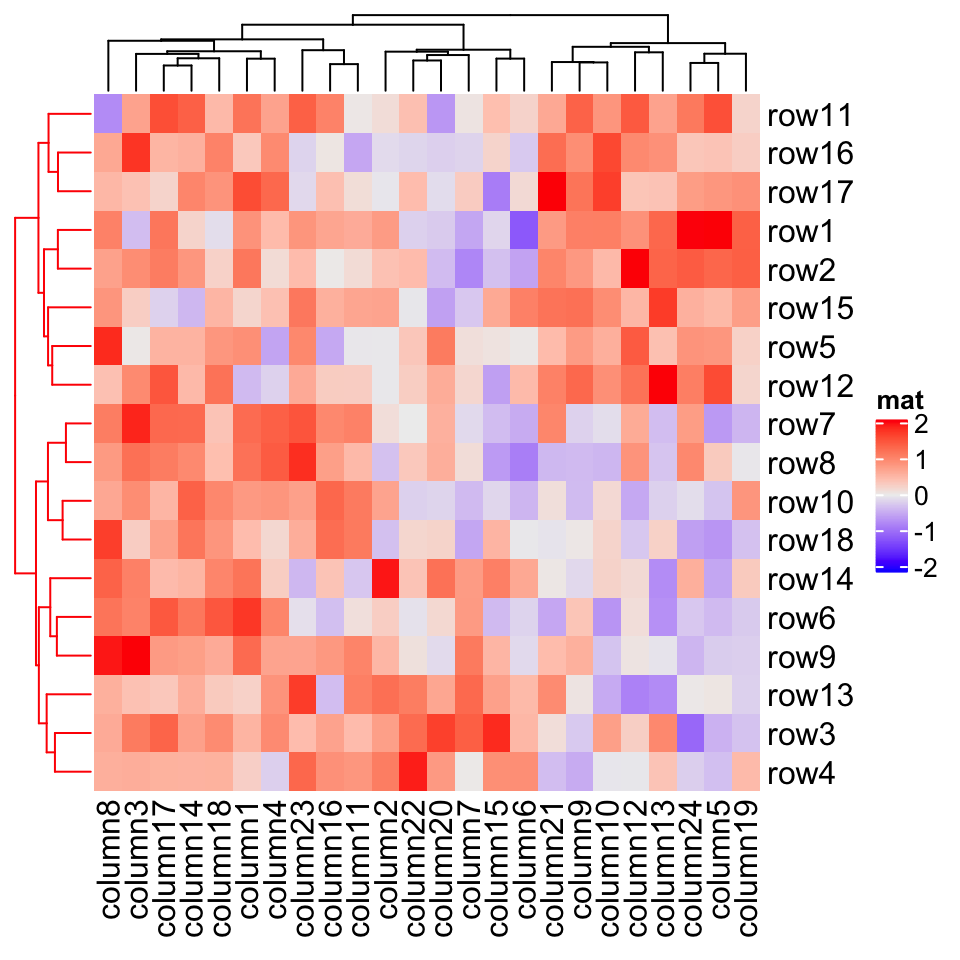
\includegraphics{02-single_heatmap_files/figure-latex/unnamed-chunk-24-1} \end{center}

For more use of the \texttt{seriate()} function, please refer to the
\href{https://cran.r-project.org/web/packages/seriation/index.html}{\textbf{seriation}
package}.

\section{Dimension names}\label{dimension-names}

The row names and column names are drawn on the right and bottom sides
of the heatmap by default. Side, visibility and graphic parameters for
dimension names can be set as follows:

\begin{Shaded}
\begin{Highlighting}[]
\KeywordTok{Heatmap}\NormalTok{(mat, }\DataTypeTok{name =} \StringTok{"mat"}\NormalTok{, }\DataTypeTok{row_names_side =} \StringTok{"left"}\NormalTok{, }\DataTypeTok{row_dend_side =} \StringTok{"right"}\NormalTok{, }
    \DataTypeTok{column_names_side =} \StringTok{"top"}\NormalTok{, }\DataTypeTok{column_dend_side =} \StringTok{"bottom"}\NormalTok{)}
\end{Highlighting}
\end{Shaded}

\begin{center}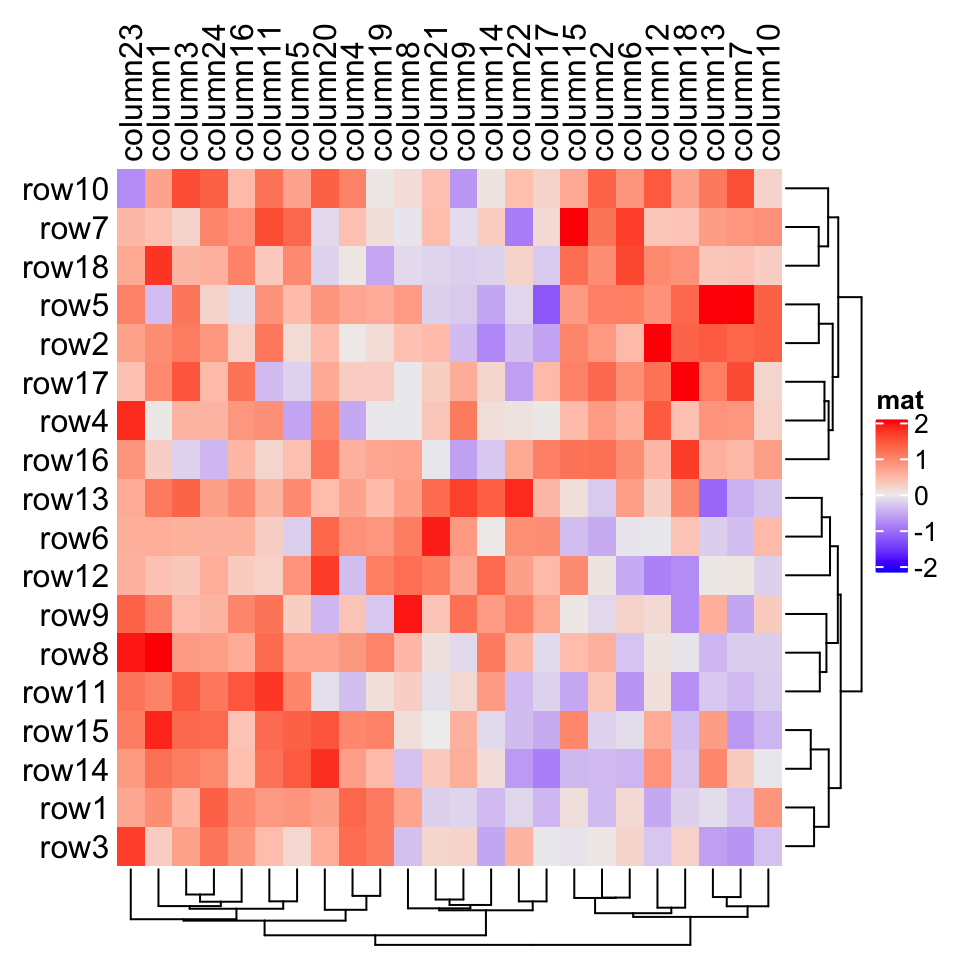
\includegraphics{02-single_heatmap_files/figure-latex/dimension_name-1} \end{center}

\begin{Shaded}
\begin{Highlighting}[]
\KeywordTok{Heatmap}\NormalTok{(mat, }\DataTypeTok{name =} \StringTok{"mat"}\NormalTok{, }\DataTypeTok{show_row_names =} \OtherTok{FALSE}\NormalTok{)}
\end{Highlighting}
\end{Shaded}

\begin{center}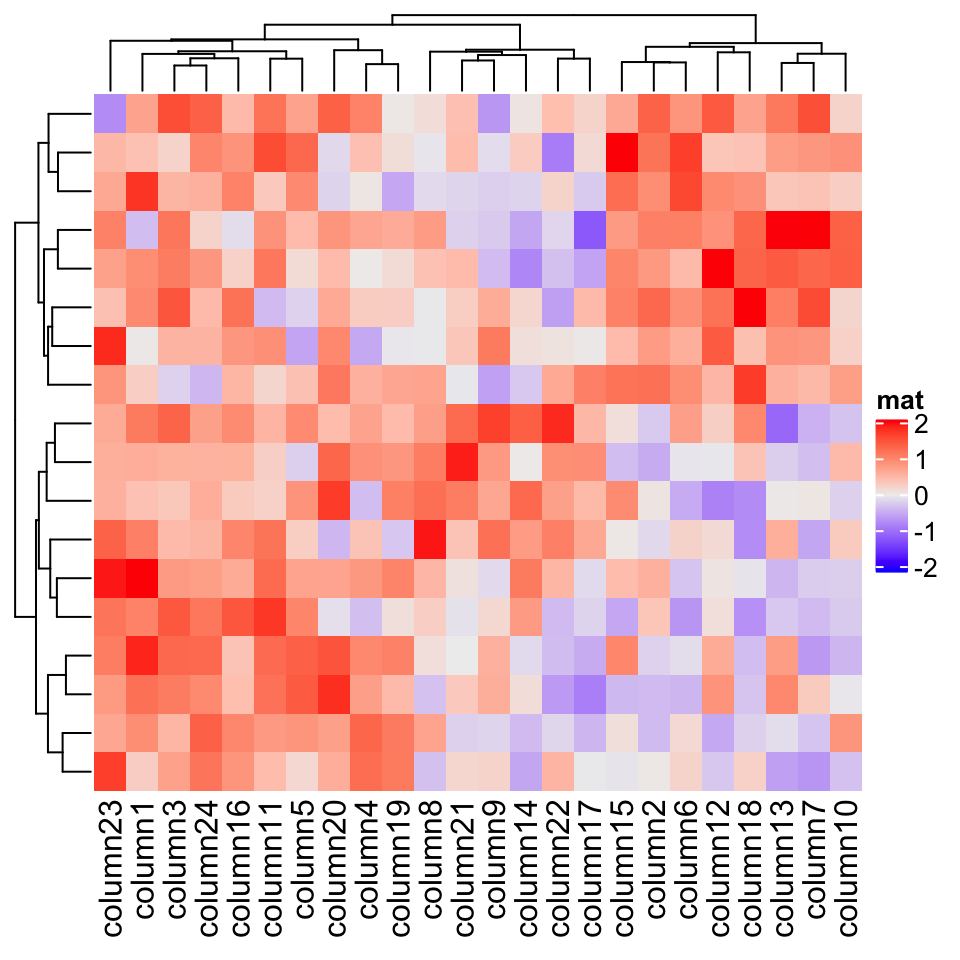
\includegraphics{02-single_heatmap_files/figure-latex/dimension_name-2} \end{center}

\begin{Shaded}
\begin{Highlighting}[]
\KeywordTok{Heatmap}\NormalTok{(mat, }\DataTypeTok{name =} \StringTok{"mat"}\NormalTok{, }\DataTypeTok{row_names_gp =} \KeywordTok{gpar}\NormalTok{(}\DataTypeTok{fontsize =} \DecValTok{20}\NormalTok{))}
\end{Highlighting}
\end{Shaded}

\begin{center}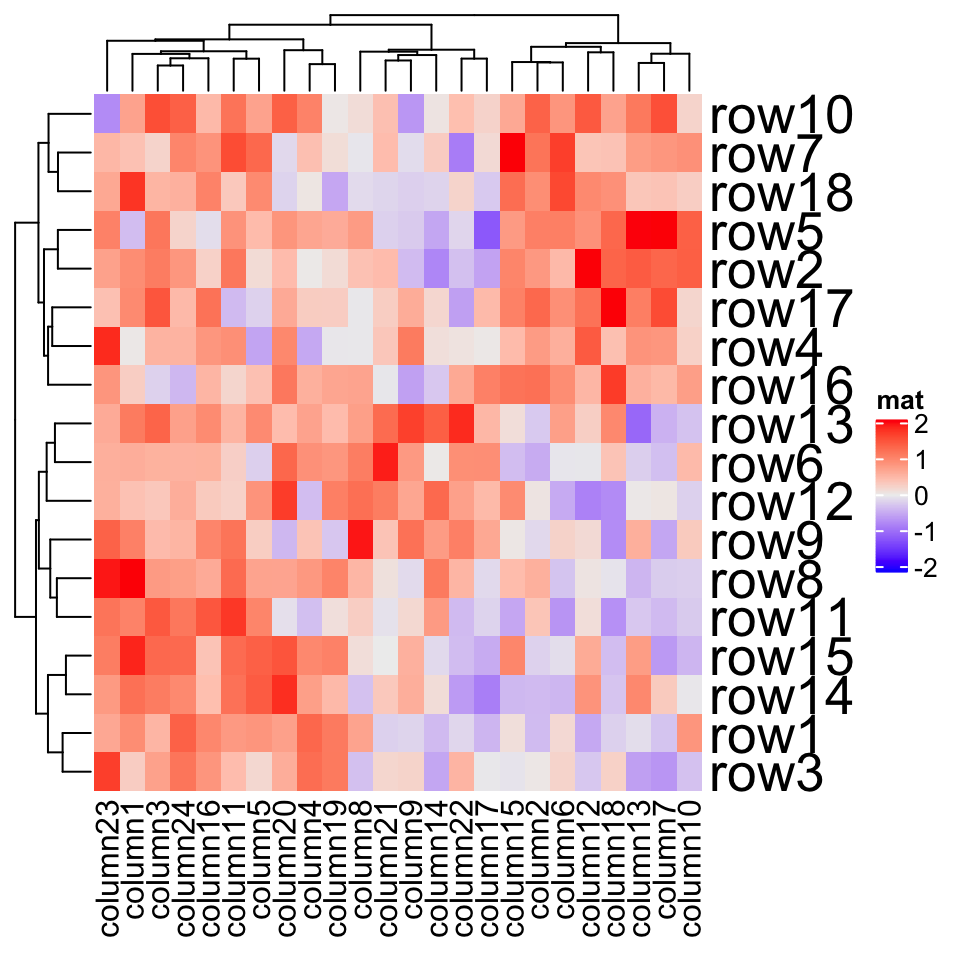
\includegraphics{02-single_heatmap_files/figure-latex/dimension_name-3} \end{center}

\begin{Shaded}
\begin{Highlighting}[]
\KeywordTok{Heatmap}\NormalTok{(mat, }\DataTypeTok{name =} \StringTok{"mat"}\NormalTok{, }\DataTypeTok{row_names_gp =} \KeywordTok{gpar}\NormalTok{(}\DataTypeTok{col =} \KeywordTok{c}\NormalTok{(}\KeywordTok{rep}\NormalTok{(}\StringTok{"red"}\NormalTok{, }\DecValTok{10}\NormalTok{), }\KeywordTok{rep}\NormalTok{(}\StringTok{"blue"}\NormalTok{, }\DecValTok{8}\NormalTok{))))}
\end{Highlighting}
\end{Shaded}

\begin{center}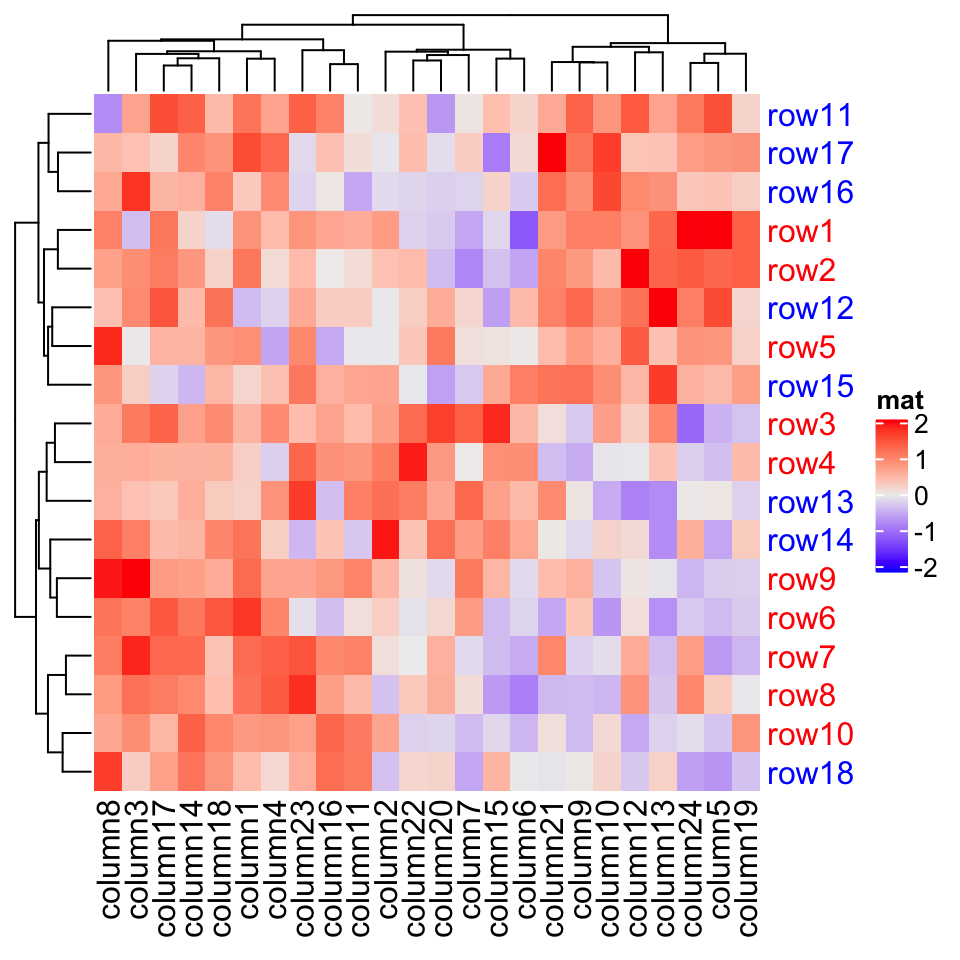
\includegraphics{02-single_heatmap_files/figure-latex/dimension_name-4} \end{center}

The rotation of column names can be set by \texttt{column\_names\_rot}:

\begin{Shaded}
\begin{Highlighting}[]
\KeywordTok{Heatmap}\NormalTok{(mat, }\DataTypeTok{name =} \StringTok{"mat"}\NormalTok{, }\DataTypeTok{column_names_rot =} \DecValTok{45}\NormalTok{)}
\KeywordTok{Heatmap}\NormalTok{(mat, }\DataTypeTok{name =} \StringTok{"mat"}\NormalTok{, }\DataTypeTok{column_names_rot =} \DecValTok{45}\NormalTok{, }\DataTypeTok{column_names_side =} \StringTok{"top"}\NormalTok{,}
    \DataTypeTok{column_dend_side =} \StringTok{"bottom"}\NormalTok{)}
\end{Highlighting}
\end{Shaded}

\begin{center}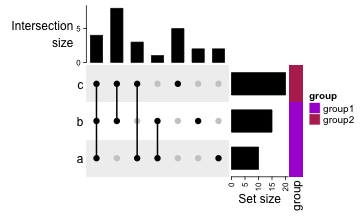
\includegraphics{02-single_heatmap_files/figure-latex/unnamed-chunk-26-1} \end{center}

If you have row names or column names which are too long,
\texttt{row\_names\_max\_width} or \texttt{column\_names\_max\_height}
can be used to set the maximal space for them.

Instead of directly using the row/column names from the matrix, you can
also provide another character vector which corresponds to the rows or
columns and set it by \texttt{row\_labels} or \texttt{column\_labels}.
This is useful because you don't need to change the dimension names of
the matrix to change the labels on the heatmap while you can directly
provide the new labels.

There is one typical scenario that \texttt{row\_labels} and
\texttt{column\_labels} are useful. For the gene expression analysis, we
might use Ensembl ID as the gene ID which is used as row names of the
gene expression matrix. However, the Ensembl ID is for the indexing of
the Ensembl database but not for the human reading. Instead, we would
prefer to put gene symbol on the heatmap as the row names which is
easier to read. To do this, we only need to assign the corresponding
gene symbols to \texttt{row\_labels} without modifying the original
matrix.

Another advantage is \texttt{row\_labels} or \texttt{column\_labels}
allows duplicated labels, while duplicated row names or column names are
not allowed in the matrix.

Following gives a simple example that we put letters as row labels and
column labels:

\begin{Shaded}
\begin{Highlighting}[]
\CommentTok{# use named vectors to make sure the correspondance between row names and row labels is correct}
\NormalTok{row_labels =}\StringTok{ }\KeywordTok{structure}\NormalTok{(}\KeywordTok{paste0}\NormalTok{(letters[}\DecValTok{1}\OperatorTok{:}\DecValTok{24}\NormalTok{], }\DecValTok{1}\OperatorTok{:}\DecValTok{24}\NormalTok{), }\DataTypeTok{names =} \KeywordTok{paste0}\NormalTok{(}\StringTok{"row"}\NormalTok{, }\DecValTok{1}\OperatorTok{:}\DecValTok{24}\NormalTok{))}
\NormalTok{column_labels =}\StringTok{ }\KeywordTok{structure}\NormalTok{(}\KeywordTok{paste0}\NormalTok{(LETTERS[}\DecValTok{1}\OperatorTok{:}\DecValTok{24}\NormalTok{], }\DecValTok{1}\OperatorTok{:}\DecValTok{24}\NormalTok{), }\DataTypeTok{names =} \KeywordTok{paste0}\NormalTok{(}\StringTok{"column"}\NormalTok{, }\DecValTok{1}\OperatorTok{:}\DecValTok{24}\NormalTok{))}
\NormalTok{row_labels}
\end{Highlighting}
\end{Shaded}

\begin{verbatim}
##  row1  row2  row3  row4  row5  row6  row7  row8  row9 row10 row11 row12 
##  "a1"  "b2"  "c3"  "d4"  "e5"  "f6"  "g7"  "h8"  "i9" "j10" "k11" "l12" 
## row13 row14 row15 row16 row17 row18 row19 row20 row21 row22 row23 row24 
## "m13" "n14" "o15" "p16" "q17" "r18" "s19" "t20" "u21" "v22" "w23" "x24"
\end{verbatim}

\begin{Shaded}
\begin{Highlighting}[]
\KeywordTok{Heatmap}\NormalTok{(mat, }\DataTypeTok{name =} \StringTok{"mat"}\NormalTok{, }\DataTypeTok{row_labels =}\NormalTok{ row_labels[}\KeywordTok{rownames}\NormalTok{(mat)], }
    \DataTypeTok{column_labels =}\NormalTok{ column_labels[}\KeywordTok{colnames}\NormalTok{(mat)])}
\end{Highlighting}
\end{Shaded}

\begin{center}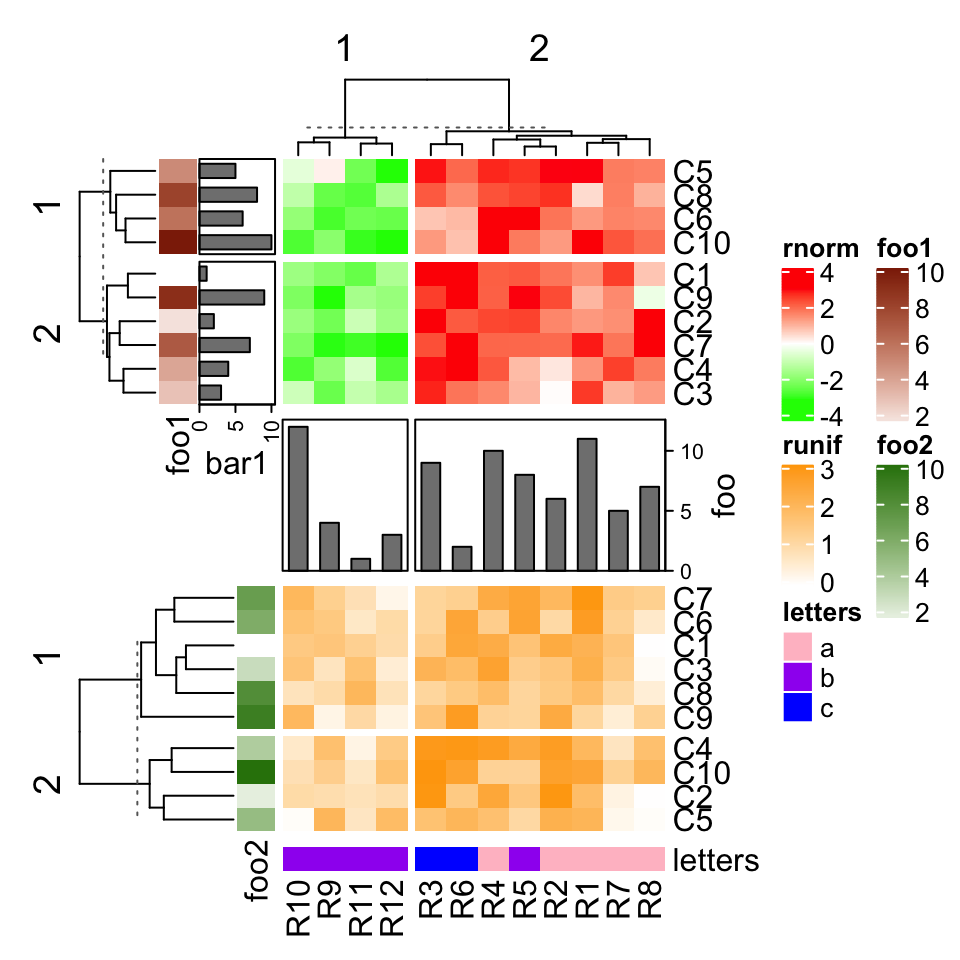
\includegraphics{02-single_heatmap_files/figure-latex/unnamed-chunk-27-1} \end{center}

\section{Heatmap split}\label{heatmap-split}

One major advantage of \textbf{ComplexHeatmap} package is it supports
splitting the heatmap by rows or/and by columns to better group the
features and additionally highlight the patterns.

Following arguments control the splitting: \texttt{row\_km},
\texttt{row\_split}, \texttt{column\_km}, \texttt{column\_split}. In
following, we call the sub-clusters generated by splitting
``\emph{slices}''.

\subsection{Split by k-means
clustering}\label{split-by-kmeans-clustering}

\texttt{row\_km} and \texttt{column\_km} apply k-means partitioning.

\begin{Shaded}
\begin{Highlighting}[]
\KeywordTok{Heatmap}\NormalTok{(mat, }\DataTypeTok{name =} \StringTok{"mat"}\NormalTok{, }\DataTypeTok{row_km =} \DecValTok{2}\NormalTok{)}
\end{Highlighting}
\end{Shaded}

\begin{center}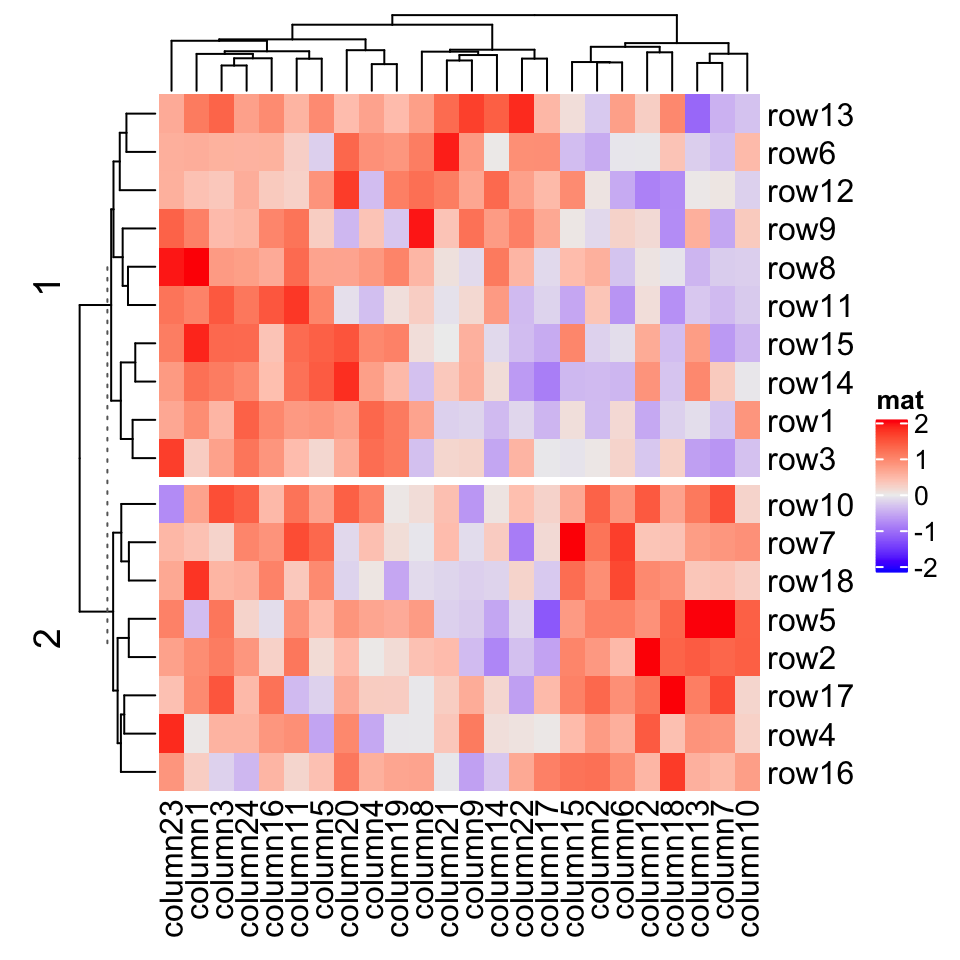
\includegraphics{02-single_heatmap_files/figure-latex/k_means-1} \end{center}

\begin{Shaded}
\begin{Highlighting}[]
\KeywordTok{Heatmap}\NormalTok{(mat, }\DataTypeTok{name =} \StringTok{"mat"}\NormalTok{, }\DataTypeTok{column_km =} \DecValTok{3}\NormalTok{)}
\end{Highlighting}
\end{Shaded}

\begin{center}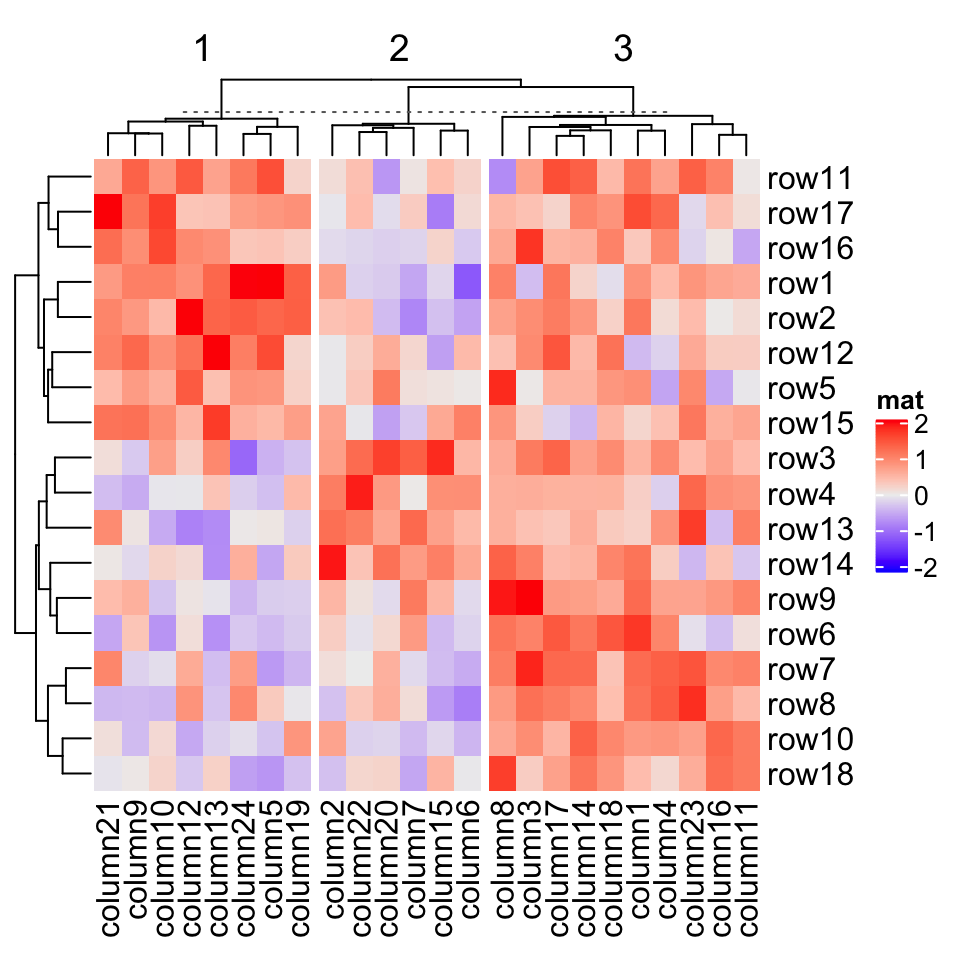
\includegraphics{02-single_heatmap_files/figure-latex/k_means-2} \end{center}

Row splitting and column splitting can be performed simultaneously.

\begin{Shaded}
\begin{Highlighting}[]
\KeywordTok{Heatmap}\NormalTok{(mat, }\DataTypeTok{name =} \StringTok{"mat"}\NormalTok{, }\DataTypeTok{row_km =} \DecValTok{2}\NormalTok{, }\DataTypeTok{column_km =} \DecValTok{3}\NormalTok{)}
\end{Highlighting}
\end{Shaded}

\begin{center}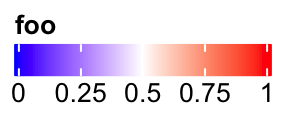
\includegraphics{02-single_heatmap_files/figure-latex/unnamed-chunk-28-1} \end{center}

\subsection{Split by categorical
variables}\label{split-by-categorical-variables}

More generally, \texttt{row\_split} or \texttt{column\_split} can be set
to a categorical vector or a data frame where different combinations of
levels split the rows/columns in the heatmap. The order of each slice
can be controlled by \texttt{levels} of each variable in \texttt{split}
(in this case, each variable should be a factor). If all variables are
characters, the default order is \texttt{unique(row\_split)} or
\texttt{unique(column\_split)}.

\begin{Shaded}
\begin{Highlighting}[]
\KeywordTok{Heatmap}\NormalTok{(mat, }\DataTypeTok{name =} \StringTok{"mat"}\NormalTok{, }
    \DataTypeTok{row_split =} \KeywordTok{rep}\NormalTok{(}\KeywordTok{c}\NormalTok{(}\StringTok{"A"}\NormalTok{, }\StringTok{"B"}\NormalTok{), }\DecValTok{9}\NormalTok{), }\DataTypeTok{column_split =} \KeywordTok{rep}\NormalTok{(}\KeywordTok{c}\NormalTok{(}\StringTok{"C"}\NormalTok{, }\StringTok{"D"}\NormalTok{), }\DecValTok{12}\NormalTok{))}
\end{Highlighting}
\end{Shaded}

\begin{center}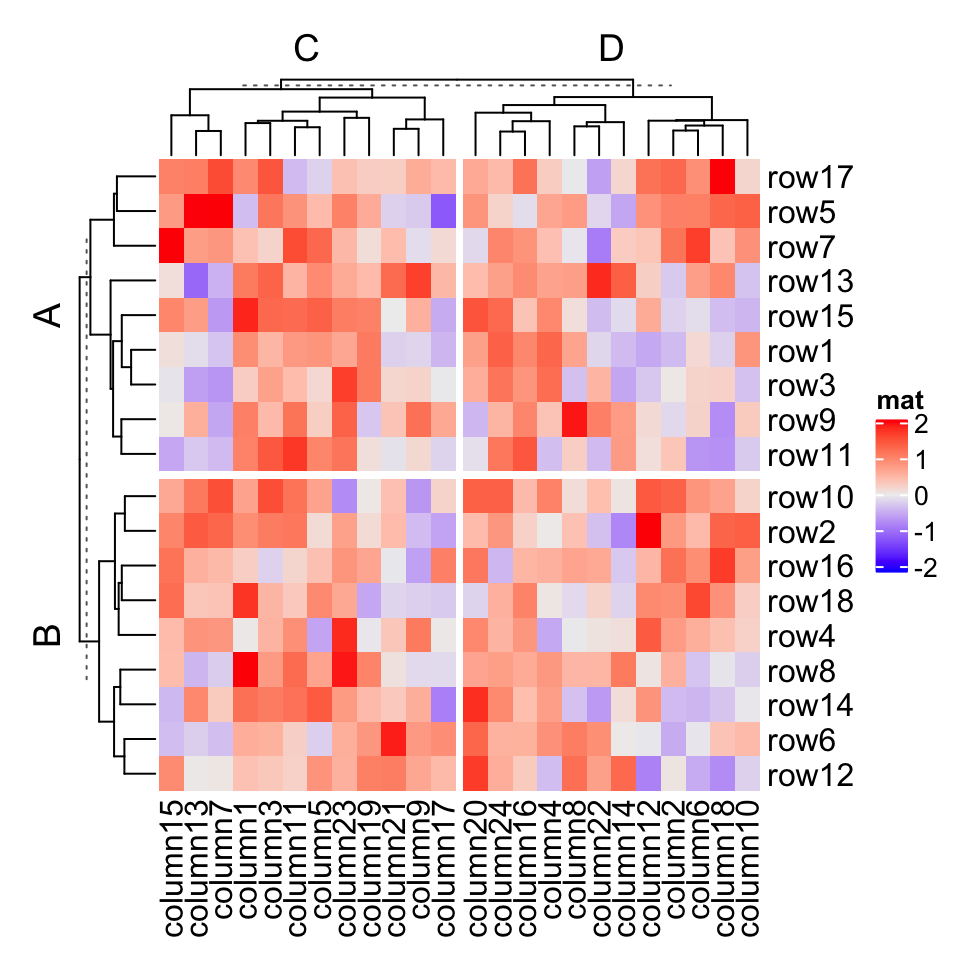
\includegraphics{02-single_heatmap_files/figure-latex/split-1} \end{center}

\begin{Shaded}
\begin{Highlighting}[]
\KeywordTok{Heatmap}\NormalTok{(mat, }\DataTypeTok{name =} \StringTok{"mat"}\NormalTok{, }
    \DataTypeTok{row_split =} \KeywordTok{data.frame}\NormalTok{(}\KeywordTok{rep}\NormalTok{(}\KeywordTok{c}\NormalTok{(}\StringTok{"A"}\NormalTok{, }\StringTok{"B"}\NormalTok{), }\DecValTok{9}\NormalTok{), }\KeywordTok{rep}\NormalTok{(}\KeywordTok{c}\NormalTok{(}\StringTok{"C"}\NormalTok{, }\StringTok{"D"}\NormalTok{), }\DataTypeTok{each =} \DecValTok{9}\NormalTok{)))}
\end{Highlighting}
\end{Shaded}

\begin{center}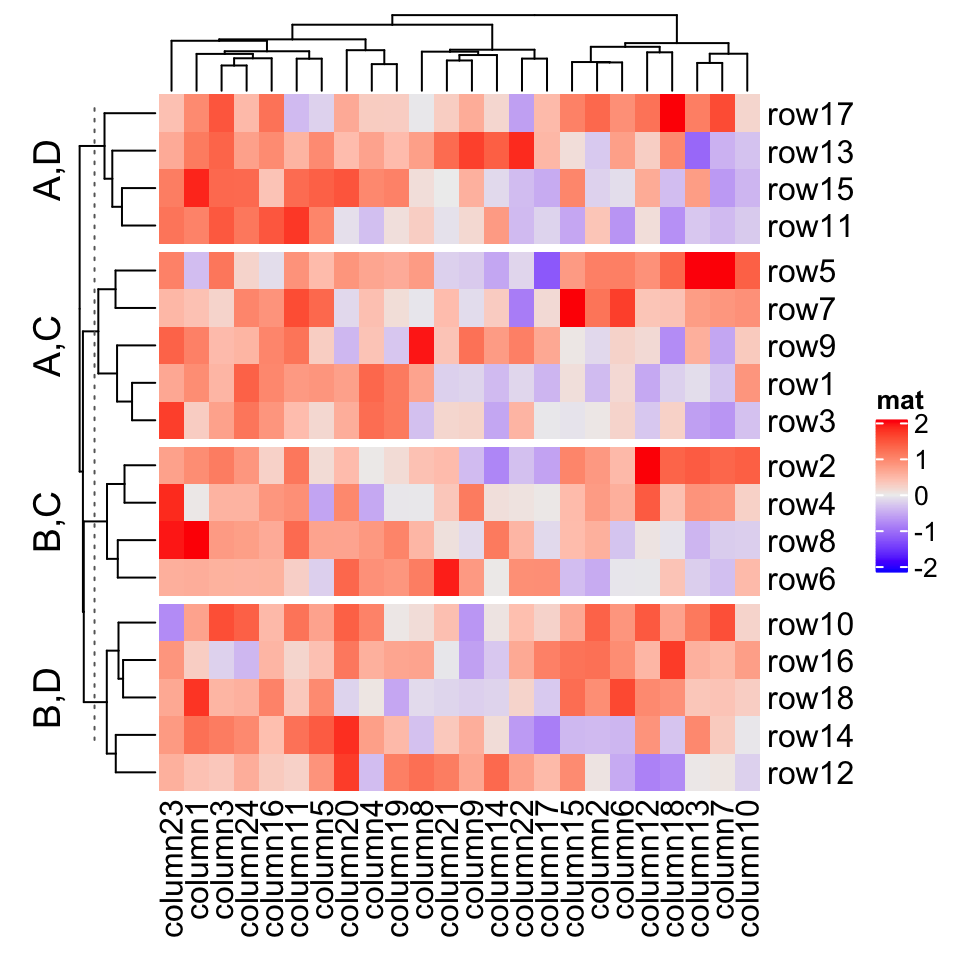
\includegraphics{02-single_heatmap_files/figure-latex/split-2} \end{center}

\begin{Shaded}
\begin{Highlighting}[]
\KeywordTok{Heatmap}\NormalTok{(mat, }\DataTypeTok{name =} \StringTok{"mat"}\NormalTok{, }\DataTypeTok{row_split =} \KeywordTok{factor}\NormalTok{(}\KeywordTok{rep}\NormalTok{(}\KeywordTok{c}\NormalTok{(}\StringTok{"A"}\NormalTok{, }\StringTok{"B"}\NormalTok{), }\DecValTok{9}\NormalTok{), }\DataTypeTok{levels =} \KeywordTok{c}\NormalTok{(}\StringTok{"B"}\NormalTok{, }\StringTok{"A"}\NormalTok{)),}
    \DataTypeTok{column_split =} \KeywordTok{factor}\NormalTok{(}\KeywordTok{rep}\NormalTok{(}\KeywordTok{c}\NormalTok{(}\StringTok{"C"}\NormalTok{, }\StringTok{"D"}\NormalTok{), }\DecValTok{12}\NormalTok{), }\DataTypeTok{levels =} \KeywordTok{c}\NormalTok{(}\StringTok{"D"}\NormalTok{, }\StringTok{"C"}\NormalTok{)))}
\end{Highlighting}
\end{Shaded}

\begin{center}\includegraphics{02-single_heatmap_files/figure-latex/split-3} \end{center}

Actually, k-means clustering just generates a vector of cluster classes
and appends to \texttt{row\_split} or \texttt{column\_split}.
\texttt{row\_km}/\texttt{column\_km} and be used mixed with
\texttt{row\_split} and \texttt{column\_split}.

\begin{Shaded}
\begin{Highlighting}[]
\KeywordTok{Heatmap}\NormalTok{(mat, }\DataTypeTok{name =} \StringTok{"mat"}\NormalTok{, }\DataTypeTok{row_split =} \KeywordTok{rep}\NormalTok{(}\KeywordTok{c}\NormalTok{(}\StringTok{"A"}\NormalTok{, }\StringTok{"B"}\NormalTok{), }\DecValTok{9}\NormalTok{), }\DataTypeTok{row_km =} \DecValTok{2}\NormalTok{)}
\end{Highlighting}
\end{Shaded}

\begin{center}\includegraphics{02-single_heatmap_files/figure-latex/unnamed-chunk-29-1} \end{center}

which is as the same as:

\begin{Shaded}
\begin{Highlighting}[]
\CommentTok{# code only for demonstration}
\NormalTok{cl =}\StringTok{ }\KeywordTok{kmeans}\NormalTok{(mat, }\DataTypeTok{centers =} \DecValTok{2}\NormalTok{)}\OperatorTok{$}\NormalTok{cluster}
\CommentTok{# classes from k-means are always put as the first column in `row_split`}
\KeywordTok{Heatmap}\NormalTok{(mat, }\DataTypeTok{name =} \StringTok{"mat"}\NormalTok{, }\DataTypeTok{row_split =} \KeywordTok{cbind}\NormalTok{(cl, }\KeywordTok{rep}\NormalTok{(}\KeywordTok{c}\NormalTok{(}\StringTok{"A"}\NormalTok{, }\StringTok{"B"}\NormalTok{), }\DecValTok{9}\NormalTok{)))}
\end{Highlighting}
\end{Shaded}

If you are not happy with the default k-means partition, it is easy to
use other partition methods by just assigning the partition vector to
\texttt{row\_split}/\texttt{column\_split}.

\begin{Shaded}
\begin{Highlighting}[]
\NormalTok{pa =}\StringTok{ }\KeywordTok{pam}\NormalTok{(mat, }\DataTypeTok{k =} \DecValTok{3}\NormalTok{)}
\KeywordTok{Heatmap}\NormalTok{(mat, }\DataTypeTok{name =} \StringTok{"mat"}\NormalTok{, }\DataTypeTok{row_split =} \KeywordTok{paste0}\NormalTok{(}\StringTok{"pam"}\NormalTok{, pa}\OperatorTok{$}\NormalTok{clustering))}
\end{Highlighting}
\end{Shaded}

\begin{center}\includegraphics{02-single_heatmap_files/figure-latex/pam-1} \end{center}

If \texttt{row\_order} or \texttt{column\_order} is set, in each
row/column slice, it is still ordered.

\begin{Shaded}
\begin{Highlighting}[]
\CommentTok{# remember when `row_order` is set, hierarchical clustering on rows is turned off}
\KeywordTok{Heatmap}\NormalTok{(mat, }\DataTypeTok{name =} \StringTok{"mat"}\NormalTok{, }\DataTypeTok{row_order =} \DecValTok{18}\OperatorTok{:}\DecValTok{1}\NormalTok{, }\DataTypeTok{row_km =} \DecValTok{2}\NormalTok{)}
\end{Highlighting}
\end{Shaded}

\begin{center}\includegraphics{02-single_heatmap_files/figure-latex/split_row_order-1} \end{center}

Character matrix can only be split by
\texttt{row\_split}/\texttt{column\_split} argument.

\begin{Shaded}
\begin{Highlighting}[]
\CommentTok{# split by the first column in `discrete_mat`}
\KeywordTok{Heatmap}\NormalTok{(discrete_mat, }\DataTypeTok{name =} \StringTok{"mat"}\NormalTok{, }\DataTypeTok{col =} \DecValTok{1}\OperatorTok{:}\DecValTok{4}\NormalTok{, }\DataTypeTok{row_split =}\NormalTok{ discrete_mat[, }\DecValTok{1}\NormalTok{])}
\end{Highlighting}
\end{Shaded}

\begin{center}\includegraphics{02-single_heatmap_files/figure-latex/split_discrete_matrix-1} \end{center}

\subsection{Split by dendrogram}\label{spilt-by-dendrogram}

In the scenarios described previously, if
\texttt{row\_km}/\texttt{column\_km} is set or
\texttt{row\_split}/\texttt{column\_split} is set as a vector or a data
frame, hierarchical clustering is first applied to each slice which
generates \texttt{k} dendrograms, then a parent dendrogram is generated
based on the mean value of each slice. \textbf{The height of the parent
dendrogram is adjusted by adding the maximal height of the dendrograms
in all children slices and the parent dendrogram is added on top of the
children dendrograms to form a single global dendrogram.}

A second scenario for splitting is that users may still want to keep the
global dendrogram which is generated from the complete matrix while not
split it in the first place. In this case,
\texttt{row\_split}/\texttt{column\_split} can be set to a single number
which will apply \texttt{cutree()} on the row/column dendrogram. This
works when \texttt{cluster\_rows}/\texttt{cluster\_columns} is set to
\texttt{TRUE} or is assigned with a \texttt{hclust}/\texttt{dendrogram}
object.

For this case, the dendrogram is still as same as the original one,
expect the positions of dendrogram leaves are slightly adjusted by the
gaps between slices.

\begin{Shaded}
\begin{Highlighting}[]
\KeywordTok{Heatmap}\NormalTok{(mat, }\DataTypeTok{name =} \StringTok{"mat"}\NormalTok{, }\DataTypeTok{row_split =} \DecValTok{2}\NormalTok{, }\DataTypeTok{column_split =} \DecValTok{3}\NormalTok{)}
\end{Highlighting}
\end{Shaded}

\begin{center}\includegraphics{02-single_heatmap_files/figure-latex/split_dendrogram-1} \end{center}

\begin{Shaded}
\begin{Highlighting}[]
\NormalTok{dend =}\StringTok{ }\KeywordTok{hclust}\NormalTok{(}\KeywordTok{dist}\NormalTok{(mat))}
\NormalTok{dend =}\StringTok{ }\KeywordTok{color_branches}\NormalTok{(dend, }\DataTypeTok{k =} \DecValTok{2}\NormalTok{)}
\KeywordTok{Heatmap}\NormalTok{(mat, }\DataTypeTok{name =} \StringTok{"mat"}\NormalTok{, }\DataTypeTok{cluster_rows =}\NormalTok{ dend, }\DataTypeTok{row_split =} \DecValTok{2}\NormalTok{)}
\end{Highlighting}
\end{Shaded}

\begin{center}\includegraphics{02-single_heatmap_files/figure-latex/split_dendrogram-2} \end{center}

If you want to combine splitting from \texttt{cutree()} and other
categorical variables, you need to generate the classes from
\texttt{cutree()} in the first place, append to e.g. \texttt{row\_split}
as a data frame and then send it to \texttt{row\_split} argument.

\begin{Shaded}
\begin{Highlighting}[]
\CommentTok{# code only for demonstration}
\NormalTok{split =}\StringTok{ }\KeywordTok{data.frame}\NormalTok{(}\KeywordTok{cutree}\NormalTok{(}\KeywordTok{hclust}\NormalTok{(}\KeywordTok{dist}\NormalTok{(mat)), }\DataTypeTok{k =} \DecValTok{2}\NormalTok{), }\KeywordTok{rep}\NormalTok{(}\KeywordTok{c}\NormalTok{(}\StringTok{"A"}\NormalTok{, }\StringTok{"B"}\NormalTok{), }\DecValTok{9}\NormalTok{))}
\KeywordTok{Heatmap}\NormalTok{(mat, }\DataTypeTok{name =} \StringTok{"mat"}\NormalTok{, }\DataTypeTok{row_split =}\NormalTok{ split)}
\end{Highlighting}
\end{Shaded}

\subsection{Titles for splitting}\label{titles-for-splitting}

When \texttt{row\_split}/\texttt{column\_split} is set as a single
number, there is only one categorical variable, while when
\texttt{row\_km}/\texttt{column\_km} is set and/or
\texttt{row\_split}/\texttt{column\_split} is set as categorical
variables, there will be multiple categorical variables. By default, the
titlea are in a form of \texttt{"level1,level2,..."} which corresponds
to every combination of levels in all categorical variables. The titles
for splitting can be controlled by ``a title template''.

\textbf{ComplexHeatmap} supports three types of templates. The first one
is by \texttt{sprintf()} where the \texttt{\%s} is replaced by the
corresponding level. In following example, since all combinations of
\texttt{split} are \texttt{A,C}, \texttt{A,D}, \texttt{B,C} and
\texttt{B,D}, if \texttt{row\_title} is set to
\texttt{\%s\textbar{}\%s}, the four row titles will be
\texttt{A\textbar{}C}, \texttt{A\textbar{}D}, \texttt{B\textbar{}C},
\texttt{B\textbar{}D}.

\begin{Shaded}
\begin{Highlighting}[]
\NormalTok{split =}\StringTok{ }\KeywordTok{data.frame}\NormalTok{(}\KeywordTok{rep}\NormalTok{(}\KeywordTok{c}\NormalTok{(}\StringTok{"A"}\NormalTok{, }\StringTok{"B"}\NormalTok{), }\DecValTok{9}\NormalTok{), }\KeywordTok{rep}\NormalTok{(}\KeywordTok{c}\NormalTok{(}\StringTok{"C"}\NormalTok{, }\StringTok{"D"}\NormalTok{), }\DataTypeTok{each =} \DecValTok{9}\NormalTok{))}
\KeywordTok{Heatmap}\NormalTok{(mat, }\DataTypeTok{name =} \StringTok{"mat"}\NormalTok{, }\DataTypeTok{row_split =}\NormalTok{ split, }\DataTypeTok{row_title =} \StringTok{"%s|%s"}\NormalTok{)}
\end{Highlighting}
\end{Shaded}

\begin{center}\includegraphics{02-single_heatmap_files/figure-latex/unnamed-chunk-32-1} \end{center}

For the \texttt{sprintf()} template, you can only put the levels which
are \texttt{A,B,C,D} in the title. However, when making the heatmap, you
might want to put more meaningful text instead of the internal levels.
Once you know how to correspond the text to the level, you can add it by
following two template methods.

In the following two template methods, special marks are used to mark
the R code which is executable (it is called variable interpolation
where the code is extracted and executed and the returned value in put
back to the string). There are two types of template marks
\texttt{@\{\}} and \texttt{\{\}}. The first one is from
\textbf{GetoptLong} package which should already be installed when you
install the \textbf{ComplexHeatmap} package and the second one is from
\textbf{glue} package which you need to install to support it.

There is an internal variable \texttt{x} you should use when you use the
latter two templates. \texttt{x} is just a simple vector which contains
current category levels (e.g. \texttt{c("A",\ "C")}).

\begin{Shaded}
\begin{Highlighting}[]
\CommentTok{# code only for demonstration}
\NormalTok{map =}\StringTok{ }\KeywordTok{c}\NormalTok{(}\StringTok{"A"}\NormalTok{ =}\StringTok{ "aaa"}\NormalTok{, }\StringTok{"B"}\NormalTok{ =}\StringTok{ "bbb"}\NormalTok{, }\StringTok{"C"}\NormalTok{ =}\StringTok{ "333"}\NormalTok{, }\StringTok{"D"}\NormalTok{ =}\StringTok{ "444"}\NormalTok{)}
\KeywordTok{Heatmap}\NormalTok{(mat, }\DataTypeTok{name =} \StringTok{"mat"}\NormalTok{, }\DataTypeTok{row_split =}\NormalTok{ split, }\DataTypeTok{row_title =} \StringTok{"@\{map[ x[1] ]\}|@\{map[ x[2] ]\}"}\NormalTok{)}
\KeywordTok{Heatmap}\NormalTok{(mat, }\DataTypeTok{name =} \StringTok{"mat"}\NormalTok{, }\DataTypeTok{row_split =}\NormalTok{ split, }\DataTypeTok{row_title =} \StringTok{"\{map[ x[1] ]\}|\{map[ x[2] ]\}"}\NormalTok{)}
\end{Highlighting}
\end{Shaded}

\begin{center}\includegraphics{02-single_heatmap_files/figure-latex/unnamed-chunk-34-1} \end{center}

The row title is rotated by default, you can set
\texttt{row\_title\_rot\ =\ 0} to make it horizontal:

\begin{Shaded}
\begin{Highlighting}[]
\KeywordTok{Heatmap}\NormalTok{(mat, }\DataTypeTok{name =} \StringTok{"mat"}\NormalTok{, }\DataTypeTok{row_split =}\NormalTok{ split, }\DataTypeTok{row_title =} \StringTok{"%s|%s"}\NormalTok{, }\DataTypeTok{row_title_rot =} \DecValTok{0}\NormalTok{)}
\end{Highlighting}
\end{Shaded}

\begin{center}\includegraphics{02-single_heatmap_files/figure-latex/unnamed-chunk-35-1} \end{center}

When \texttt{row\_split}/\texttt{column\_split} is set as a number, you
can also use template to adjust the titles for slices.

\begin{Shaded}
\begin{Highlighting}[]
\KeywordTok{Heatmap}\NormalTok{(mat, }\DataTypeTok{name =} \StringTok{"mat"}\NormalTok{, }\DataTypeTok{row_split =} \DecValTok{2}\NormalTok{, }\DataTypeTok{row_title =} \StringTok{"cluster_%s"}\NormalTok{)}
\end{Highlighting}
\end{Shaded}

\begin{center}\includegraphics{02-single_heatmap_files/figure-latex/unnamed-chunk-36-1} \end{center}

If you know the final number of row slices, you can directly set a
vector of titles to \texttt{row\_title}. Be careful the number of row
slices is not always identical to \texttt{nlevel\_1*nlevel\_2*...}.

\begin{Shaded}
\begin{Highlighting}[]
\KeywordTok{Heatmap}\NormalTok{(mat, }\DataTypeTok{name =} \StringTok{"mat"}\NormalTok{, }\DataTypeTok{row_split =}\NormalTok{ split, }
    \DataTypeTok{row_title =} \KeywordTok{c}\NormalTok{(}\StringTok{"top_slice"}\NormalTok{, }\StringTok{"middle_top_slice"}\NormalTok{, }\StringTok{"middle_bottom_slice"}\NormalTok{, }\StringTok{"bottom_slice"}\NormalTok{),}
    \DataTypeTok{row_title_rot =} \DecValTok{0}\NormalTok{)}
\end{Highlighting}
\end{Shaded}

\begin{center}\includegraphics{02-single_heatmap_files/figure-latex/unnamed-chunk-37-1} \end{center}

If the length of \texttt{row\_title} is specified as a single string, it
will be like a title for all slices.

\begin{Shaded}
\begin{Highlighting}[]
\KeywordTok{Heatmap}\NormalTok{(mat, }\DataTypeTok{name =} \StringTok{"mat"}\NormalTok{, }\DataTypeTok{row_split =}\NormalTok{ split, }\DataTypeTok{row_title =} \StringTok{"there are four slices"}\NormalTok{)}
\end{Highlighting}
\end{Shaded}

\begin{center}\includegraphics{02-single_heatmap_files/figure-latex/unnamed-chunk-38-1} \end{center}

If you still want titles for each slice, but also a global title, you
can do as follows.

\begin{Shaded}
\begin{Highlighting}[]
\NormalTok{ht =}\StringTok{ }\KeywordTok{Heatmap}\NormalTok{(mat, }\DataTypeTok{name =} \StringTok{"mat"}\NormalTok{, }\DataTypeTok{row_split =}\NormalTok{ split, }\DataTypeTok{row_title =} \StringTok{"%s|%s"}\NormalTok{)}
\KeywordTok{draw}\NormalTok{(ht, }\DataTypeTok{row_title =} \StringTok{"I am a row title"}\NormalTok{)}
\end{Highlighting}
\end{Shaded}

\begin{center}\includegraphics{02-single_heatmap_files/figure-latex/unnamed-chunk-39-1} \end{center}

Actually the \texttt{row\_title} used in \texttt{draw()} function is the
row title of the heatmap list, although in the example there is only one
heatmap. The \texttt{draw()} function and the heatmap list will be
introduced in Chapter \ref{a-list-of-heatmaps}.

If \texttt{row\_title} is set to \texttt{NULL} or \texttt{""}, no row
title will be drawn.

\begin{Shaded}
\begin{Highlighting}[]
\KeywordTok{Heatmap}\NormalTok{(mat, }\DataTypeTok{name =} \StringTok{"mat"}\NormalTok{, }\DataTypeTok{row_split =}\NormalTok{ split, }\DataTypeTok{row_title =} \OtherTok{NULL}\NormalTok{)}
\end{Highlighting}
\end{Shaded}

\begin{center}\includegraphics{02-single_heatmap_files/figure-latex/unnamed-chunk-40-1} \end{center}

\subsection{Graphic parameters for
splitting}\label{graphic-parameters-for-splitting}

When splitting is applied on rows/columns, graphic parameters for
row/column title and row/column names can be specified as same length as
number of slices.

\begin{Shaded}
\begin{Highlighting}[]
\KeywordTok{Heatmap}\NormalTok{(mat, }\DataTypeTok{name =} \StringTok{"mat"}\NormalTok{, }
    \DataTypeTok{row_km =} \DecValTok{2}\NormalTok{, }\DataTypeTok{row_title_gp =} \KeywordTok{gpar}\NormalTok{(}\DataTypeTok{col =} \KeywordTok{c}\NormalTok{(}\StringTok{"red"}\NormalTok{, }\StringTok{"blue"}\NormalTok{), }\DataTypeTok{font =} \DecValTok{1}\OperatorTok{:}\DecValTok{2}\NormalTok{),}
    \DataTypeTok{row_names_gp =} \KeywordTok{gpar}\NormalTok{(}\DataTypeTok{col =} \KeywordTok{c}\NormalTok{(}\StringTok{"green"}\NormalTok{, }\StringTok{"orange"}\NormalTok{), }\DataTypeTok{fontsize =} \KeywordTok{c}\NormalTok{(}\DecValTok{10}\NormalTok{, }\DecValTok{14}\NormalTok{)),}
    \DataTypeTok{column_km =} \DecValTok{3}\NormalTok{, }\DataTypeTok{column_title_gp =} \KeywordTok{gpar}\NormalTok{(}\DataTypeTok{col =} \KeywordTok{c}\NormalTok{(}\StringTok{"red"}\NormalTok{, }\StringTok{"blue"}\NormalTok{, }\StringTok{"green"}\NormalTok{), }\DataTypeTok{font =} \DecValTok{1}\OperatorTok{:}\DecValTok{3}\NormalTok{),}
    \DataTypeTok{column_names_gp =} \KeywordTok{gpar}\NormalTok{(}\DataTypeTok{col =} \KeywordTok{c}\NormalTok{(}\StringTok{"green"}\NormalTok{, }\StringTok{"orange"}\NormalTok{, }\StringTok{"purple"}\NormalTok{), }\DataTypeTok{fontsize =} \KeywordTok{c}\NormalTok{(}\DecValTok{10}\NormalTok{, }\DecValTok{14}\NormalTok{, }\DecValTok{8}\NormalTok{)))}
\end{Highlighting}
\end{Shaded}

\begin{center}\includegraphics{02-single_heatmap_files/figure-latex/split_graphical_parameter-1} \end{center}

\subsection{Gaps between slices}\label{gaps-between-slices}

The space of gaps between row/column slices can be controlled by
\texttt{row\_gap}/\texttt{column\_gap}. The value can be a single unit
or a vector of units.

\begin{Shaded}
\begin{Highlighting}[]
\KeywordTok{Heatmap}\NormalTok{(mat, }\DataTypeTok{name =} \StringTok{"mat"}\NormalTok{, }\DataTypeTok{row_km =} \DecValTok{3}\NormalTok{, }\DataTypeTok{row_gap =} \KeywordTok{unit}\NormalTok{(}\DecValTok{5}\NormalTok{, }\StringTok{"mm"}\NormalTok{))}
\end{Highlighting}
\end{Shaded}

\begin{center}\includegraphics{02-single_heatmap_files/figure-latex/split_gap-1} \end{center}

\begin{Shaded}
\begin{Highlighting}[]
\KeywordTok{Heatmap}\NormalTok{(mat, }\DataTypeTok{name =} \StringTok{"mat"}\NormalTok{, }\DataTypeTok{row_km =} \DecValTok{3}\NormalTok{, }\DataTypeTok{row_gap =} \KeywordTok{unit}\NormalTok{(}\KeywordTok{c}\NormalTok{(}\DecValTok{2}\NormalTok{, }\DecValTok{4}\NormalTok{), }\StringTok{"mm"}\NormalTok{))}
\end{Highlighting}
\end{Shaded}

\begin{center}\includegraphics{02-single_heatmap_files/figure-latex/split_gap-2} \end{center}

\begin{Shaded}
\begin{Highlighting}[]
\KeywordTok{Heatmap}\NormalTok{(mat, }\DataTypeTok{name =} \StringTok{"mat"}\NormalTok{, }\DataTypeTok{row_km =} \DecValTok{3}\NormalTok{, }\DataTypeTok{row_gap =} \KeywordTok{unit}\NormalTok{(}\KeywordTok{c}\NormalTok{(}\DecValTok{2}\NormalTok{, }\DecValTok{4}\NormalTok{), }\StringTok{"mm"}\NormalTok{),}
    \DataTypeTok{column_km =} \DecValTok{3}\NormalTok{, }\DataTypeTok{column_gap =} \KeywordTok{unit}\NormalTok{(}\KeywordTok{c}\NormalTok{(}\DecValTok{2}\NormalTok{, }\DecValTok{4}\NormalTok{), }\StringTok{"mm"}\NormalTok{))}
\end{Highlighting}
\end{Shaded}

\begin{center}\includegraphics{02-single_heatmap_files/figure-latex/split_gap-3} \end{center}

When heatmap border is added by setting \texttt{border\ =\ TRUE}, the
border of every slice is added.

\begin{Shaded}
\begin{Highlighting}[]
\KeywordTok{Heatmap}\NormalTok{(mat, }\DataTypeTok{name =} \StringTok{"mat"}\NormalTok{, }\DataTypeTok{row_km =} \DecValTok{2}\NormalTok{, }\DataTypeTok{column_km =} \DecValTok{3}\NormalTok{, }\DataTypeTok{border =} \OtherTok{TRUE}\NormalTok{)}
\end{Highlighting}
\end{Shaded}

\begin{center}\includegraphics{02-single_heatmap_files/figure-latex/unnamed-chunk-41-1} \end{center}

If you set gap size to zero, the heatmap will look like it is
partitioned by vertical and horizontal lines.

\begin{Shaded}
\begin{Highlighting}[]
\KeywordTok{Heatmap}\NormalTok{(mat, }\DataTypeTok{name =} \StringTok{"mat"}\NormalTok{, }\DataTypeTok{row_km =} \DecValTok{2}\NormalTok{, }\DataTypeTok{column_km =} \DecValTok{3}\NormalTok{, }
    \DataTypeTok{row_gap =} \KeywordTok{unit}\NormalTok{(}\DecValTok{0}\NormalTok{, }\StringTok{"mm"}\NormalTok{), }\DataTypeTok{column_gap =} \KeywordTok{unit}\NormalTok{(}\DecValTok{0}\NormalTok{, }\StringTok{"mm"}\NormalTok{), }\DataTypeTok{border =} \OtherTok{TRUE}\NormalTok{)}
\end{Highlighting}
\end{Shaded}

\begin{center}\includegraphics{02-single_heatmap_files/figure-latex/unnamed-chunk-42-1} \end{center}

\subsection{Split heatmap annotations}\label{split-heatmap-annotations}

When the heatmap is split, all the heatmap components are split
accordingly. Following gives you a simple example and the heatmap
annotation will be introduced in Chapter \ref{heatmap-annotations}.

\begin{Shaded}
\begin{Highlighting}[]
\KeywordTok{Heatmap}\NormalTok{(mat, }\DataTypeTok{name =} \StringTok{"mat"}\NormalTok{, }\DataTypeTok{row_km =} \DecValTok{2}\NormalTok{, }\DataTypeTok{column_km =} \DecValTok{3}\NormalTok{,}
    \DataTypeTok{top_annotation =} \KeywordTok{HeatmapAnnotation}\NormalTok{(}\DataTypeTok{foo1 =} \DecValTok{1}\OperatorTok{:}\DecValTok{24}\NormalTok{, }\DataTypeTok{bar1 =} \KeywordTok{anno_points}\NormalTok{(}\KeywordTok{runif}\NormalTok{(}\DecValTok{24}\NormalTok{))),}
    \DataTypeTok{right_annotation =} \KeywordTok{rowAnnotation}\NormalTok{(}\DataTypeTok{foo2 =} \DecValTok{18}\OperatorTok{:}\DecValTok{1}\NormalTok{, }\DataTypeTok{bar2 =} \KeywordTok{anno_barplot}\NormalTok{(}\KeywordTok{runif}\NormalTok{(}\DecValTok{18}\NormalTok{)))}
\NormalTok{)}
\end{Highlighting}
\end{Shaded}

\begin{center}\includegraphics{02-single_heatmap_files/figure-latex/unnamed-chunk-43-1} \end{center}

\section{Heatmap as raster image}\label{heatmap-as-raster-image}

Saving plots in PDF format is kind like best parctice to preserve the
quality. However, when there are too many rows (say, \textgreater{}
10000), the output PDF file would be huge and it takes long time and
memory to read the whole plot. On the other hand, details of the huge
matrix will not be seen in limited size of PDF file. Rendering heatmaps
(the heatmap body) as raster images will effectively reduce the file
size while the plot looks exactly the same for your screen or if you
print it out. In \texttt{Heatmap()} function, there are four options
which control how to generate the raster image: \texttt{use\_raster},
\texttt{raster\_device}, \texttt{raster\_quality},
\texttt{raster\_device\_param}.

You can choose graphic device (\texttt{png}, \texttt{jpeg} and
\texttt{tiff}) by \texttt{raster\_device}, control the quality of the
raster image by \texttt{raster\_quality}, and pass further parameters
for a specific device by \texttt{raster\_device\_param}.

If \texttt{raster\_quality} is set to 1, internally, a PNG (if
\texttt{raster\_device} is set to \texttt{png}) file is generated with
the same physical size as the heatmap body and refit into the heatmap
body as a raster image. The png file generated has the size of
\texttt{raster\_quality*width} and \texttt{raster\_quality*height}. So a
larger \texttt{raster\_quality} value gives you a better reservation of
the original resolution.

In \textbf{Complexheatmap}, \texttt{use\_raster} is by default turned on
if the number of rows or columns is more than 2000.

\begin{Shaded}
\begin{Highlighting}[]
\CommentTok{# code only for demonstration}
\KeywordTok{Heatmap}\NormalTok{(mat, }\DataTypeTok{use_raster =} \OtherTok{TRUE}\NormalTok{, }\DataTypeTok{raster_quality =} \DecValTok{2}\NormalTok{)}
\end{Highlighting}
\end{Shaded}

\section{Customize the heatmap body}\label{customize-the-heatmap-body}

The heatmap body can be self-defined to add more types of graphics. By
default the heatmap body is composed by an array of rectangles (it might
be called grids in other parts of this documentation, but it is called
``\emph{cells}'' here) with different filled colors. However, it is also
possible to add more graphics or symbols as additional layers on the
heatmap. There are two arguments \texttt{cell\_fun} and
\texttt{layer\_fun} which both should be user-defined functions.

\texttt{cell\_fun} draws in each cell repeatedly, which is internally
executed in two nested \texttt{for} loops, while \texttt{layer\_fun} is
the vectorized version of \texttt{cell\_fun}. \texttt{cell\_fun} is
easier to understand but \texttt{layer\_fun} is faster to execute.

\texttt{cell\_fun} expects a function with 7 arguments (the argument
names can be different from following, but the order must be the same),
which are:

\begin{itemize}
\tightlist
\item
  \texttt{j}: column index in the matrix. Column index corresponds to
  the x-direction in the viewport, that's why \texttt{j} is put as the
  first argument.
\item
  \texttt{i}: row index in the matrix.
\item
  \texttt{x}: x coordinate of middle point of the cell which is measured
  in the viewport of the heatmap body.
\item
  \texttt{y}: y coordinate of middle point of the cell which is measured
  in the viewport of the heatmap body.
\item
  \texttt{width}: width of the cell. The value is
  \texttt{unit(1/ncol(mat),\ "npc")}.
\item
  \texttt{height}: height of the cell. The value is
  \texttt{unit(1/nrow(mat),\ "npc")}.
\item
  \texttt{fill}: color of the cell.
\end{itemize}

The values for the seven arguments are automatically sent to the
function when executed in each cell.

The most common use is to add values in the matrix onto the heatmap:

\begin{Shaded}
\begin{Highlighting}[]
\NormalTok{small_mat =}\StringTok{ }\NormalTok{mat[}\DecValTok{1}\OperatorTok{:}\DecValTok{9}\NormalTok{, }\DecValTok{1}\OperatorTok{:}\DecValTok{9}\NormalTok{]}
\NormalTok{col_fun =}\StringTok{ }\KeywordTok{colorRamp2}\NormalTok{(}\KeywordTok{c}\NormalTok{(}\OperatorTok{-}\DecValTok{2}\NormalTok{, }\DecValTok{0}\NormalTok{, }\DecValTok{2}\NormalTok{), }\KeywordTok{c}\NormalTok{(}\StringTok{"green"}\NormalTok{, }\StringTok{"white"}\NormalTok{, }\StringTok{"red"}\NormalTok{))}
\KeywordTok{Heatmap}\NormalTok{(small_mat, }\DataTypeTok{name =} \StringTok{"mat"}\NormalTok{, }\DataTypeTok{col =}\NormalTok{ col_fun,}
    \DataTypeTok{cell_fun =} \ControlFlowTok{function}\NormalTok{(j, i, x, y, width, height, fill) \{}
        \KeywordTok{grid.text}\NormalTok{(}\KeywordTok{sprintf}\NormalTok{(}\StringTok{"%.1f"}\NormalTok{, mat[i, j]), x, y, }\DataTypeTok{gp =} \KeywordTok{gpar}\NormalTok{(}\DataTypeTok{fontsize =} \DecValTok{10}\NormalTok{))}
\NormalTok{\})}
\end{Highlighting}
\end{Shaded}

\begin{center}\includegraphics{02-single_heatmap_files/figure-latex/unnamed-chunk-45-1} \end{center}

and we can also choose only to add text for the cells with positive
values:

\begin{Shaded}
\begin{Highlighting}[]
\KeywordTok{Heatmap}\NormalTok{(small_mat, }\DataTypeTok{name =} \StringTok{"mat"}\NormalTok{,  }\DataTypeTok{col =}\NormalTok{ col_fun,}
    \DataTypeTok{cell_fun =} \ControlFlowTok{function}\NormalTok{(j, i, x, y, width, height, fill) \{}
        \ControlFlowTok{if}\NormalTok{(small_mat[i, j] }\OperatorTok{>}\StringTok{ }\DecValTok{0}\NormalTok{)}
            \KeywordTok{grid.text}\NormalTok{(}\KeywordTok{sprintf}\NormalTok{(}\StringTok{"%.1f"}\NormalTok{, mat[i, j]), x, y, }\DataTypeTok{gp =} \KeywordTok{gpar}\NormalTok{(}\DataTypeTok{fontsize =} \DecValTok{10}\NormalTok{))}
\NormalTok{\})}
\end{Highlighting}
\end{Shaded}

\begin{center}\includegraphics{02-single_heatmap_files/figure-latex/unnamed-chunk-46-1} \end{center}

In following example, we make a heatmap which shows correlation matrix
similar as the \textbf{corrplot} package:

\begin{Shaded}
\begin{Highlighting}[]
\NormalTok{cor_mat =}\StringTok{ }\KeywordTok{cor}\NormalTok{(small_mat)}
\NormalTok{od =}\StringTok{ }\KeywordTok{hclust}\NormalTok{(}\KeywordTok{dist}\NormalTok{(cor_mat))}\OperatorTok{$}\NormalTok{order}
\NormalTok{cor_mat =}\StringTok{ }\NormalTok{cor_mat[od, od]}
\NormalTok{nm =}\StringTok{ }\KeywordTok{rownames}\NormalTok{(cor_mat)}
\NormalTok{col_fun =}\StringTok{ }\NormalTok{circlize}\OperatorTok{::}\KeywordTok{colorRamp2}\NormalTok{(}\KeywordTok{c}\NormalTok{(}\OperatorTok{-}\DecValTok{1}\NormalTok{, }\DecValTok{0}\NormalTok{, }\DecValTok{1}\NormalTok{), }\KeywordTok{c}\NormalTok{(}\StringTok{"green"}\NormalTok{, }\StringTok{"white"}\NormalTok{, }\StringTok{"red"}\NormalTok{))}
\CommentTok{# `col = col_fun` here is used to generate the legend}
\KeywordTok{Heatmap}\NormalTok{(cor_mat, }\DataTypeTok{name =} \StringTok{"correlation"}\NormalTok{, }\DataTypeTok{col =}\NormalTok{ col_fun, }\DataTypeTok{rect_gp =} \KeywordTok{gpar}\NormalTok{(}\DataTypeTok{type =} \StringTok{"none"}\NormalTok{), }
    \DataTypeTok{cell_fun =} \ControlFlowTok{function}\NormalTok{(j, i, x, y, width, height, fill) \{}
        \KeywordTok{grid.rect}\NormalTok{(}\DataTypeTok{x =}\NormalTok{ x, }\DataTypeTok{y =}\NormalTok{ y, }\DataTypeTok{width =}\NormalTok{ width, }\DataTypeTok{height =}\NormalTok{ height, }\DataTypeTok{gp =} \KeywordTok{gpar}\NormalTok{(}\DataTypeTok{col =} \StringTok{"grey"}\NormalTok{, }\DataTypeTok{fill =} \OtherTok{NA}\NormalTok{))}
        \ControlFlowTok{if}\NormalTok{(i }\OperatorTok{==}\StringTok{ }\NormalTok{j) \{}
            \KeywordTok{grid.text}\NormalTok{(nm[i], }\DataTypeTok{x =}\NormalTok{ x, }\DataTypeTok{y =}\NormalTok{ y)}
\NormalTok{        \} }\ControlFlowTok{else} \ControlFlowTok{if}\NormalTok{(i }\OperatorTok{>}\StringTok{ }\NormalTok{j) \{}
            \KeywordTok{grid.circle}\NormalTok{(}\DataTypeTok{x =}\NormalTok{ x, }\DataTypeTok{y =}\NormalTok{ y, }\DataTypeTok{r =} \KeywordTok{abs}\NormalTok{(cor_mat[i, j])}\OperatorTok{/}\DecValTok{2} \OperatorTok{*}\StringTok{ }\KeywordTok{min}\NormalTok{(}\KeywordTok{unit.c}\NormalTok{(width, height)), }
                \DataTypeTok{gp =} \KeywordTok{gpar}\NormalTok{(}\DataTypeTok{fill =} \KeywordTok{col_fun}\NormalTok{(cor_mat[i, j]), }\DataTypeTok{col =} \OtherTok{NA}\NormalTok{))}
\NormalTok{        \} }\ControlFlowTok{else}\NormalTok{ \{}
            \KeywordTok{grid.text}\NormalTok{(}\KeywordTok{sprintf}\NormalTok{(}\StringTok{"%.1f"}\NormalTok{, cor_mat[i, j]), x, y, }\DataTypeTok{gp =} \KeywordTok{gpar}\NormalTok{(}\DataTypeTok{fontsize =} \DecValTok{10}\NormalTok{))}
\NormalTok{        \}}
\NormalTok{    \}, }\DataTypeTok{cluster_rows =} \OtherTok{FALSE}\NormalTok{, }\DataTypeTok{cluster_columns =} \OtherTok{FALSE}\NormalTok{,}
    \DataTypeTok{show_row_names =} \OtherTok{FALSE}\NormalTok{, }\DataTypeTok{show_column_names =} \OtherTok{FALSE}\NormalTok{)}
\end{Highlighting}
\end{Shaded}

\begin{center}\includegraphics{02-single_heatmap_files/figure-latex/cell_fun-1} \end{center}

As you may see, when setting the non-standard parameter
\texttt{rect\_gp\ =\ gpar(type\ =\ "none")}, the clustering is performed
but nothing is drawn on the heatmap body.

Similar as \texttt{cell\_fun}, \texttt{layer\_fun} also needs seven
arguments, but they are all in vector form:

\begin{Shaded}
\begin{Highlighting}[]
\CommentTok{# code only for demonstration}
\KeywordTok{Heatmap}\NormalTok{(..., }\DataTypeTok{layer_fun =} \ControlFlowTok{function}\NormalTok{(j, i, x, y, w, h, fill) \{...\})}
\CommentTok{# on you can capitalize the arguments to mark they are vectors}
\KeywordTok{Heatmap}\NormalTok{(..., }\DataTypeTok{layer_fun =} \ControlFlowTok{function}\NormalTok{(J, I, X, Y, W, H, F) \{...\})}
\end{Highlighting}
\end{Shaded}

Since \texttt{j} and \texttt{i} are vectors, to get corresponding values
in the matrix, we cannot use the form as \texttt{mat{[}j,\ i{]}} because
it gives you a sub-matrix with \texttt{length(i)} rows and
\texttt{length(j)} columns, instead we can use \texttt{pindex()}
function from \textbf{ComplexHeatmap} which is like pairwise indexing.
See follow example:

\begin{Shaded}
\begin{Highlighting}[]
\NormalTok{mfoo =}\StringTok{ }\KeywordTok{matrix}\NormalTok{(}\DecValTok{1}\OperatorTok{:}\DecValTok{9}\NormalTok{, }\DataTypeTok{nr =} \DecValTok{3}\NormalTok{)}
\NormalTok{mfoo[}\DecValTok{1}\OperatorTok{:}\DecValTok{2}\NormalTok{, }\KeywordTok{c}\NormalTok{(}\DecValTok{1}\NormalTok{, }\DecValTok{3}\NormalTok{)]}
\end{Highlighting}
\end{Shaded}

\begin{verbatim}
##      [,1] [,2]
## [1,]    1    7
## [2,]    2    8
\end{verbatim}

\begin{Shaded}
\begin{Highlighting}[]
\CommentTok{# but we actually want mfoo[1, 1] and mfoo[2, 3]}
\KeywordTok{pindex}\NormalTok{(mfoo, }\DecValTok{1}\OperatorTok{:}\DecValTok{2}\NormalTok{, }\KeywordTok{c}\NormalTok{(}\DecValTok{1}\NormalTok{, }\DecValTok{3}\NormalTok{))}
\end{Highlighting}
\end{Shaded}

\begin{verbatim}
## [1] 1 8
\end{verbatim}

Next example shows the \texttt{layer\_fun} version of adding text on
heatmap. It's basically the same as the \texttt{cell\_fun} version.

\begin{Shaded}
\begin{Highlighting}[]
\NormalTok{col_fun =}\StringTok{ }\KeywordTok{colorRamp2}\NormalTok{(}\KeywordTok{c}\NormalTok{(}\OperatorTok{-}\DecValTok{2}\NormalTok{, }\DecValTok{0}\NormalTok{, }\DecValTok{2}\NormalTok{), }\KeywordTok{c}\NormalTok{(}\StringTok{"green"}\NormalTok{, }\StringTok{"white"}\NormalTok{, }\StringTok{"red"}\NormalTok{))}
\KeywordTok{Heatmap}\NormalTok{(small_mat, }\DataTypeTok{name =} \StringTok{"mat"}\NormalTok{, }\DataTypeTok{col =}\NormalTok{ col_fun,}
    \DataTypeTok{layer_fun =} \ControlFlowTok{function}\NormalTok{(j, i, x, y, width, height, fill) \{}
        \CommentTok{# since grid.text can also be vectorized}
        \KeywordTok{grid.text}\NormalTok{(}\KeywordTok{sprintf}\NormalTok{(}\StringTok{"%.1f"}\NormalTok{, }\KeywordTok{pindex}\NormalTok{(mat, i, j)), x, y, }\DataTypeTok{gp =} \KeywordTok{gpar}\NormalTok{(}\DataTypeTok{fontsize =} \DecValTok{10}\NormalTok{))}
\NormalTok{\})}
\end{Highlighting}
\end{Shaded}

\begin{center}\includegraphics{02-single_heatmap_files/figure-latex/unnamed-chunk-49-1} \end{center}

And only add text to cells with positive values:

\begin{Shaded}
\begin{Highlighting}[]
\KeywordTok{Heatmap}\NormalTok{(small_mat, }\DataTypeTok{name =} \StringTok{"mat"}\NormalTok{, }\DataTypeTok{col =}\NormalTok{ col_fun, }
    \DataTypeTok{layer_fun =} \ControlFlowTok{function}\NormalTok{(j, i, x, y, width, height, fill) \{}
\NormalTok{        v =}\StringTok{ }\KeywordTok{pindex}\NormalTok{(mat, i, j)}
\NormalTok{        l =}\StringTok{ }\NormalTok{v }\OperatorTok{>}\StringTok{ }\DecValTok{0}
        \KeywordTok{grid.text}\NormalTok{(}\KeywordTok{sprintf}\NormalTok{(}\StringTok{"%.1f"}\NormalTok{, v[l]), x[l], y[l], }\DataTypeTok{gp =} \KeywordTok{gpar}\NormalTok{(}\DataTypeTok{fontsize =} \DecValTok{10}\NormalTok{))}
\NormalTok{\})}
\end{Highlighting}
\end{Shaded}

\begin{center}\includegraphics{02-single_heatmap_files/figure-latex/unnamed-chunk-50-1} \end{center}

One last example is to visualize a
\href{https://en.wikipedia.org/wiki/Go_\%28game\%29}{GO game}. The input
data takes records of moves in the game.

\begin{Shaded}
\begin{Highlighting}[]
\NormalTok{str =}\StringTok{ "B[cp];W[pq];B[dc];W[qd];B[eq];W[od];B[de];W[jc];B[qk];W[qn]}
\StringTok{;B[qh];W[ck];B[ci];W[cn];B[hc];W[je];B[jq];W[df];B[ee];W[cf]}
\StringTok{;B[ei];W[bc];B[ce];W[be];B[bd];W[cd];B[bf];W[ad];B[bg];W[cc]}
\StringTok{;B[eb];W[db];B[ec];W[lq];B[nq];W[jp];B[iq];W[kq];B[pp];W[op]}
\StringTok{;B[po];W[oq];B[rp];W[ql];B[oo];W[no];B[pl];W[pm];B[np];W[qq]}
\StringTok{;B[om];W[ol];B[pk];W[qp];B[on];W[rm];B[mo];W[nr];B[rl];W[rk]}
\StringTok{;B[qm];W[dp];B[dq];W[ql];B[or];W[mp];B[nn];W[mq];B[qm];W[bp]}
\StringTok{;B[co];W[ql];B[no];W[pr];B[qm];W[dd];B[pn];W[ed];B[bo];W[eg]}
\StringTok{;B[ef];W[dg];B[ge];W[gh];B[gf];W[gg];B[ek];W[ig];B[fd];W[en]}
\StringTok{;B[bn];W[ip];B[dm];W[ff];B[cb];W[fe];B[hp];W[ho];B[hq];W[el]}
\StringTok{;B[dl];W[fk];B[ej];W[fp];B[go];W[hn];B[fo];W[em];B[dn];W[eo]}
\StringTok{;B[gp];W[ib];B[gc];W[pg];B[qg];W[ng];B[qc];W[re];B[pf];W[of]}
\StringTok{;B[rc];W[ob];B[ph];W[qo];B[rn];W[mi];B[og];W[oe];B[qe];W[rd]}
\StringTok{;B[rf];W[pd];B[gm];W[gl];B[fm];W[fl];B[lj];W[mj];B[lk];W[ro]}
\StringTok{;B[hl];W[hk];B[ik];W[dk];B[bi];W[di];B[dj];W[dh];B[hj];W[gj]}
\StringTok{;B[li];W[lh];B[kh];W[lg];B[jn];W[do];B[cl];W[ij];B[gk];W[bl]}
\StringTok{;B[cm];W[hk];B[jk];W[lo];B[hi];W[hm];B[gk];W[bm];B[cn];W[hk]}
\StringTok{;B[il];W[cq];B[bq];W[ii];B[sm];W[jo];B[kn];W[fq];B[ep];W[cj]}
\StringTok{;B[bk];W[er];B[cr];W[gr];B[gk];W[fj];B[ko];W[kp];B[hr];W[jr]}
\StringTok{;B[nh];W[mh];B[mk];W[bb];B[da];W[jh];B[ic];W[id];B[hb];W[jb]}
\StringTok{;B[oj];W[fn];B[fs];W[fr];B[gs];W[es];B[hs];W[gn];B[kr];W[is]}
\StringTok{;B[dr];W[fi];B[bj];W[hd];B[gd];W[ln];B[lm];W[oi];B[oh];W[ni]}
\StringTok{;B[pi];W[ki];B[kj];W[ji];B[so];W[rq];B[if];W[jf];B[hh];W[hf]}
\StringTok{;B[he];W[ie];B[hg];W[ba];B[ca];W[sp];B[im];W[sn];B[rm];W[pe]}
\StringTok{;B[qf];W[if];B[hk];W[nj];B[nk];W[lr];B[mn];W[af];B[ag];W[ch]}
\StringTok{;B[bh];W[lp];B[ia];W[ja];B[ha];W[sf];B[sg];W[se];B[eh];W[fh]}
\StringTok{;B[in];W[ih];B[ae];W[so];B[af]"}
\end{Highlighting}
\end{Shaded}

We convert it into a matrix:

\begin{Shaded}
\begin{Highlighting}[]
\NormalTok{str =}\StringTok{ }\KeywordTok{gsub}\NormalTok{(}\StringTok{"}\CharTok{\textbackslash{}\textbackslash{}}\StringTok{n"}\NormalTok{, }\StringTok{""}\NormalTok{, str)}
\NormalTok{step =}\StringTok{ }\KeywordTok{strsplit}\NormalTok{(str, }\StringTok{";"}\NormalTok{)[[}\DecValTok{1}\NormalTok{]]}
\NormalTok{type =}\StringTok{ }\KeywordTok{gsub}\NormalTok{(}\StringTok{"(B|W).*"}\NormalTok{, }\StringTok{"}\CharTok{\textbackslash{}\textbackslash{}}\StringTok{1"}\NormalTok{, step)}
\NormalTok{row =}\StringTok{ }\KeywordTok{gsub}\NormalTok{(}\StringTok{"(B|W)}\CharTok{\textbackslash{}\textbackslash{}}\StringTok{[(.).}\CharTok{\textbackslash{}\textbackslash{}}\StringTok{]"}\NormalTok{, }\StringTok{"}\CharTok{\textbackslash{}\textbackslash{}}\StringTok{2"}\NormalTok{, step)}
\NormalTok{column =}\StringTok{ }\KeywordTok{gsub}\NormalTok{(}\StringTok{"(B|W)}\CharTok{\textbackslash{}\textbackslash{}}\StringTok{[.(.)}\CharTok{\textbackslash{}\textbackslash{}}\StringTok{]"}\NormalTok{, }\StringTok{"}\CharTok{\textbackslash{}\textbackslash{}}\StringTok{2"}\NormalTok{, step)}

\NormalTok{go_mat =}\StringTok{ }\KeywordTok{matrix}\NormalTok{(}\DataTypeTok{nrow =} \DecValTok{19}\NormalTok{, }\DataTypeTok{ncol =} \DecValTok{19}\NormalTok{)}
\KeywordTok{rownames}\NormalTok{(go_mat) =}\StringTok{ }\NormalTok{letters[}\DecValTok{1}\OperatorTok{:}\DecValTok{19}\NormalTok{]}
\KeywordTok{colnames}\NormalTok{(go_mat) =}\StringTok{ }\NormalTok{letters[}\DecValTok{1}\OperatorTok{:}\DecValTok{19}\NormalTok{]}
\ControlFlowTok{for}\NormalTok{(i }\ControlFlowTok{in} \KeywordTok{seq_along}\NormalTok{(row)) \{}
\NormalTok{    go_mat[row[i], column[i]] =}\StringTok{ }\NormalTok{type[i]}
\NormalTok{\}}
\NormalTok{go_mat[}\DecValTok{1}\OperatorTok{:}\DecValTok{4}\NormalTok{, }\DecValTok{1}\OperatorTok{:}\DecValTok{4}\NormalTok{]}
\end{Highlighting}
\end{Shaded}

\begin{verbatim}
##   a   b   c   d  
## a NA  NA  NA  "W"
## b "W" "W" "W" "B"
## c "B" "B" "W" "W"
## d "B" "W" "B" "W"
\end{verbatim}

Black and white stones are put based on the values in the matrix:

\begin{Shaded}
\begin{Highlighting}[]
\KeywordTok{Heatmap}\NormalTok{(go_mat, }\DataTypeTok{name =} \StringTok{"go"}\NormalTok{, }\DataTypeTok{rect_gp =} \KeywordTok{gpar}\NormalTok{(}\DataTypeTok{type =} \StringTok{"none"}\NormalTok{),}
    \DataTypeTok{cell_fun =} \ControlFlowTok{function}\NormalTok{(j, i, x, y, w, h, col) \{}
        \KeywordTok{grid.rect}\NormalTok{(x, y, w, h, }\DataTypeTok{gp =} \KeywordTok{gpar}\NormalTok{(}\DataTypeTok{fill =} \StringTok{"#dcb35c"}\NormalTok{, }\DataTypeTok{col =} \OtherTok{NA}\NormalTok{))}
        \ControlFlowTok{if}\NormalTok{(i }\OperatorTok{==}\StringTok{ }\DecValTok{1}\NormalTok{) \{}
            \KeywordTok{grid.segments}\NormalTok{(x, y}\OperatorTok{-}\NormalTok{h}\OperatorTok{*}\FloatTok{0.5}\NormalTok{, x, y)}
\NormalTok{        \} }\ControlFlowTok{else} \ControlFlowTok{if}\NormalTok{(i }\OperatorTok{==}\StringTok{ }\KeywordTok{nrow}\NormalTok{(go_mat)) \{}
            \KeywordTok{grid.segments}\NormalTok{(x, y, x, y}\OperatorTok{+}\NormalTok{h}\OperatorTok{*}\FloatTok{0.5}\NormalTok{)}
\NormalTok{        \} }\ControlFlowTok{else}\NormalTok{ \{}
            \KeywordTok{grid.segments}\NormalTok{(x, y}\OperatorTok{-}\NormalTok{h}\OperatorTok{*}\FloatTok{0.5}\NormalTok{, x, y}\OperatorTok{+}\NormalTok{h}\OperatorTok{*}\FloatTok{0.5}\NormalTok{)}
\NormalTok{        \}}
        \ControlFlowTok{if}\NormalTok{(j }\OperatorTok{==}\StringTok{ }\DecValTok{1}\NormalTok{) \{}
            \KeywordTok{grid.segments}\NormalTok{(x, y, x}\OperatorTok{+}\NormalTok{w}\OperatorTok{*}\FloatTok{0.5}\NormalTok{, y)        }
\NormalTok{        \} }\ControlFlowTok{else} \ControlFlowTok{if}\NormalTok{(j }\OperatorTok{==}\StringTok{ }\KeywordTok{ncol}\NormalTok{(go_mat)) \{}
            \KeywordTok{grid.segments}\NormalTok{(x}\OperatorTok{-}\NormalTok{w}\OperatorTok{*}\FloatTok{0.5}\NormalTok{, y, x, y)}
\NormalTok{        \} }\ControlFlowTok{else}\NormalTok{ \{}
            \KeywordTok{grid.segments}\NormalTok{(x}\OperatorTok{-}\NormalTok{w}\OperatorTok{*}\FloatTok{0.5}\NormalTok{, y, x}\OperatorTok{+}\NormalTok{w}\OperatorTok{*}\FloatTok{0.5}\NormalTok{, y)}
\NormalTok{        \}}

        \ControlFlowTok{if}\NormalTok{(i }\OperatorTok\StringTok{ }\KeywordTok{c}\NormalTok{(}\DecValTok{4}\NormalTok{, }\DecValTok{10}\NormalTok{, }\DecValTok{16}\NormalTok{) }\OperatorTok{&}\StringTok{ }\NormalTok{j }\OperatorTok\StringTok{ }\KeywordTok{c}\NormalTok{(}\DecValTok{4}\NormalTok{, }\DecValTok{10}\NormalTok{, }\DecValTok{16}\NormalTok{)) \{}
            \KeywordTok{grid.points}\NormalTok{(x, y, }\DataTypeTok{pch =} \DecValTok{16}\NormalTok{, }\DataTypeTok{size =} \KeywordTok{unit}\NormalTok{(}\DecValTok{2}\NormalTok{, }\StringTok{"mm"}\NormalTok{))}
\NormalTok{        \}}
                
\NormalTok{        r =}\StringTok{ }\KeywordTok{min}\NormalTok{(}\KeywordTok{unit.c}\NormalTok{(w, h))}\OperatorTok{*}\FloatTok{0.45}
        \ControlFlowTok{if}\NormalTok{(}\KeywordTok{is.na}\NormalTok{(go_mat[i, j])) \{}
\NormalTok{        \} }\ControlFlowTok{else} \ControlFlowTok{if}\NormalTok{(go_mat[i, j] }\OperatorTok{==}\StringTok{ "W"}\NormalTok{) \{}
            \KeywordTok{grid.circle}\NormalTok{(x, y, r, }\DataTypeTok{gp =} \KeywordTok{gpar}\NormalTok{(}\DataTypeTok{fill =} \StringTok{"white"}\NormalTok{, }\DataTypeTok{col =} \StringTok{"white"}\NormalTok{))}
\NormalTok{        \} }\ControlFlowTok{else} \ControlFlowTok{if}\NormalTok{(go_mat[i, j] }\OperatorTok{==}\StringTok{ "B"}\NormalTok{) \{}
            \KeywordTok{grid.circle}\NormalTok{(x, y, r, }\DataTypeTok{gp =} \KeywordTok{gpar}\NormalTok{(}\DataTypeTok{fill =} \StringTok{"black"}\NormalTok{, }\DataTypeTok{col =} \StringTok{"black"}\NormalTok{))}
\NormalTok{        \}}
\NormalTok{    \},}
    \DataTypeTok{col =} \KeywordTok{c}\NormalTok{(}\StringTok{"B"}\NormalTok{ =}\StringTok{ "black"}\NormalTok{, }\StringTok{"W"}\NormalTok{ =}\StringTok{ "white"}\NormalTok{),}
    \DataTypeTok{show_row_names =} \OtherTok{FALSE}\NormalTok{, }\DataTypeTok{show_column_names =} \OtherTok{FALSE}\NormalTok{,}
    \DataTypeTok{column_title =} \StringTok{"One famous GO game"}\NormalTok{,}
    \DataTypeTok{heatmap_legend_param =} \KeywordTok{list}\NormalTok{(}\DataTypeTok{title =} \StringTok{"Player"}\NormalTok{, }\DataTypeTok{at =} \KeywordTok{c}\NormalTok{(}\StringTok{"B"}\NormalTok{, }\StringTok{"W"}\NormalTok{), }
        \DataTypeTok{labels =} \KeywordTok{c}\NormalTok{(}\StringTok{"player1"}\NormalTok{, }\StringTok{"player2"}\NormalTok{), }\DataTypeTok{border =} \StringTok{"black"}\NormalTok{)}
\NormalTok{)}
\end{Highlighting}
\end{Shaded}

\begin{center}\includegraphics{02-single_heatmap_files/figure-latex/unnamed-chunk-53-1} \end{center}

\section{Size of the heatmap}\label{size-of-the-heatmap}

\texttt{width}, \texttt{heatmap\_width}, \texttt{height} and
\texttt{heatmap\_height} control the size of the heatmap. By default,
all heatmap components have fixed width or height, e.g.~the width of row
dendrogram is \texttt{1cm}. The width or the height of the heatmap body
fill the rest area of the final plotting region, which means, if you
draw it in an interactive graphic window and you change the size of the
window by draging it, the size of the heatmap body is automatically
adjusted.

\texttt{heatmap\_width} and \texttt{heatmap\_height} control the
width/height of the complete heatmap while \texttt{width} and
\texttt{height} only control the width/height of the heamtap body. All
these four arguments can be set as absolute units.

\begin{Shaded}
\begin{Highlighting}[]
\KeywordTok{Heatmap}\NormalTok{(mat, }\DataTypeTok{name =} \StringTok{"mat"}\NormalTok{, }\DataTypeTok{width =} \KeywordTok{unit}\NormalTok{(}\DecValTok{10}\NormalTok{, }\StringTok{"cm"}\NormalTok{), }\DataTypeTok{height =} \KeywordTok{unit}\NormalTok{(}\DecValTok{10}\NormalTok{, }\StringTok{"cm"}\NormalTok{))}
\end{Highlighting}
\end{Shaded}

\begin{center}\includegraphics{02-single_heatmap_files/figure-latex/unnamed-chunk-54-1} \end{center}

\begin{verbatim}
## Since all heatmaps/annotations have absolute units, the total width of the plot is 139mm
## Since all heatmaps/annotations have absolute units, the total height of the plot is 135mm
\end{verbatim}

\begin{Shaded}
\begin{Highlighting}[]
\KeywordTok{Heatmap}\NormalTok{(mat, }\DataTypeTok{name =} \StringTok{"mat"}\NormalTok{, }\DataTypeTok{heatmap_width =} \KeywordTok{unit}\NormalTok{(}\DecValTok{10}\NormalTok{, }\StringTok{"cm"}\NormalTok{), }\DataTypeTok{heatmap_height =} \KeywordTok{unit}\NormalTok{(}\DecValTok{10}\NormalTok{, }\StringTok{"cm"}\NormalTok{))}
\end{Highlighting}
\end{Shaded}

\begin{center}\includegraphics{02-single_heatmap_files/figure-latex/unnamed-chunk-54-2} \end{center}

\begin{verbatim}
## Since all heatmaps/annotations have absolute units, the total width of the plot is 115mm
## Since all heatmaps/annotations have absolute units, the total height of the plot is 104mm
\end{verbatim}

There will be message showing the size of the whole plot.

These four arguments are more important when adjust the size in a list
of heatmaps (see Section \ref{size-of-heatmaps}).

\section{Plot the heatmap
\{plot-the-heatmap\}}\label{plot-the-heatmap-plot-the-heatmap}

\texttt{Heatmap()} function actually is only a constructor, which means
it only puts all the data and configurations into the object in the
\texttt{Heatmap} class. The clustering will only be performed when the
\texttt{draw()} method is called. Under interactive mode (e.g.~the
interactive R terminal where you can type your R code line by line),
directly calling \texttt{Heatmap()} without returning to any object
prints the object and the print method (or the S4 \texttt{show()}
method) for the \texttt{Heatmap} class object calls \texttt{draw()}
internally. So if you type \texttt{Heatmap(...)} in your R terminal, it
looks like it is a plotting function like \texttt{plot()}, you need to
be aware of that it is actually not true and in the following cases you
might see nothing plotted.

\begin{itemize}
\tightlist
\item
  you put \texttt{Heatmap(...)} inside a function,
\item
  you put \texttt{Heatmap(...)} in a code chunk like \texttt{for} or
  \texttt{if-else}
\item
  you put \texttt{Heatmap(...)} in an Rscript and you run it under
  command line.
\end{itemize}

The reason is in above three cases, the \texttt{show()} method WILL NOT
be called and thus \texttt{draw()} method is not executed either. So, to
make the plot, you need to call \texttt{draw()} explicitly:
\texttt{draw(Heatmap(...))} or:

\begin{Shaded}
\begin{Highlighting}[]
\CommentTok{# code only for demonstration}
\NormalTok{ht =}\StringTok{ }\KeywordTok{Heatmap}\NormalTok{(...)}
\KeywordTok{draw}\NormalTok{(ht)}
\end{Highlighting}
\end{Shaded}

The \texttt{draw()} function actually is applied to a list of heatmaps
in \texttt{HeatmapList} class. The \texttt{draw()} method for the single
\texttt{Heatmap} class constructs a \texttt{HeatmapList} with only one
heatmap and call \texttt{draw()} method of the \texttt{HeatmapList}
class. The \texttt{draw()} function accpets a lot of more arguments
which e.g.~controls the legends. It will be discussed in Chapter
\ref{a-list-of-heatmaps}.

\begin{Shaded}
\begin{Highlighting}[]
\KeywordTok{draw}\NormalTok{(ht, heatmap_legend_side, padding, ...)}
\end{Highlighting}
\end{Shaded}

\section{Get orders and
dendrograms}\label{get-orders-and-dendrograms-from-heatmap}

The row/column orders of the heatmap can be obtained by
\texttt{row\_order()}/\texttt{column\_order()} functions. You can
directly apply to the heatmap object returned by \texttt{Heatmap()} or
to the object returned by \texttt{draw()}. In following, we take
\texttt{row\_order()} as example.

\begin{Shaded}
\begin{Highlighting}[]
\NormalTok{small_mat =}\StringTok{ }\NormalTok{mat[}\DecValTok{1}\OperatorTok{:}\DecValTok{9}\NormalTok{, }\DecValTok{1}\OperatorTok{:}\DecValTok{9}\NormalTok{]}
\NormalTok{ht1 =}\StringTok{ }\KeywordTok{Heatmap}\NormalTok{(small_mat)}
\KeywordTok{row_order}\NormalTok{(ht1)}
\end{Highlighting}
\end{Shaded}

\begin{verbatim}
## [1] 9 6 7 8 3 4 2 5 1
\end{verbatim}

\begin{Shaded}
\begin{Highlighting}[]
\NormalTok{ht2 =}\StringTok{ }\KeywordTok{draw}\NormalTok{(ht1)}
\KeywordTok{row_order}\NormalTok{(ht2)}
\end{Highlighting}
\end{Shaded}

\begin{verbatim}
## [1] 9 6 7 8 3 4 2 5 1
\end{verbatim}

As explained in previous section, \texttt{Heatmap()} function does not
perform clustering, thus, when directly apply \texttt{row\_order()} on
\texttt{ht1}, clustering will be performed. Later when making the
heatmap by \texttt{draw(ht1)}, the clustering will be applied again.
This might be a problem that if you set k-means clustering in the
heatmap. Since the clustering is applied twice, k-means might give you
different clustering, which means, you might have different results from
\texttt{row\_order()} and you might have different heatmap.

In following chunk of code, \texttt{o1}, \texttt{o2} and \texttt{o3}
might be different because each time, k-means clustering is performed.

\begin{Shaded}
\begin{Highlighting}[]
\NormalTok{ht1 =}\StringTok{ }\KeywordTok{Heatmap}\NormalTok{(small_mat, }\DataTypeTok{row_km =} \DecValTok{2}\NormalTok{)}
\NormalTok{o1 =}\StringTok{ }\KeywordTok{row_order}\NormalTok{(ht1)}
\NormalTok{o2 =}\StringTok{ }\KeywordTok{row_order}\NormalTok{(ht1)}
\NormalTok{ht2 =}\StringTok{ }\KeywordTok{draw}\NormalTok{(ht1)}
\NormalTok{o3 =}\StringTok{ }\KeywordTok{row_order}\NormalTok{(ht2)}
\NormalTok{o4 =}\StringTok{ }\KeywordTok{row_order}\NormalTok{(ht2)}
\end{Highlighting}
\end{Shaded}

\texttt{draw()} function returns the heatmap (or more precisely, the
heatmap list) which has been reordered, and applying
\texttt{row\_order()} just extracts the row order from the object, which
ensures the row order is exactly the same as the one shown in the
heatmap. In above code, \texttt{o3} is always identical to \texttt{o4}.

So, the preferable way to get row/column orders is as follows.

\begin{Shaded}
\begin{Highlighting}[]
\CommentTok{# code only for demonstration}
\NormalTok{ht =}\StringTok{ }\KeywordTok{Heatmap}\NormalTok{(small_mat)}
\NormalTok{ht =}\StringTok{ }\KeywordTok{draw}\NormalTok{(ht)}
\KeywordTok{row_order}\NormalTok{(ht)}
\KeywordTok{column_order}\NormalTok{(ht)}
\end{Highlighting}
\end{Shaded}

If rows/columns are split, row order or column order will be a list.

\begin{Shaded}
\begin{Highlighting}[]
\NormalTok{ht =}\StringTok{ }\KeywordTok{Heatmap}\NormalTok{(small_mat, }\DataTypeTok{row_km =} \DecValTok{2}\NormalTok{, }\DataTypeTok{column_km =} \DecValTok{3}\NormalTok{)}
\NormalTok{ht =}\StringTok{ }\KeywordTok{draw}\NormalTok{(ht)}
\KeywordTok{row_order}\NormalTok{(ht)}
\end{Highlighting}
\end{Shaded}

\begin{verbatim}
## $`1`
## [1] 9 6 7 8 3 4
## 
## $`2`
## [1] 2 5 1
\end{verbatim}

\begin{Shaded}
\begin{Highlighting}[]
\KeywordTok{column_order}\NormalTok{(ht)}
\end{Highlighting}
\end{Shaded}

\begin{verbatim}
## $`1`
## [1] 5 9
## 
## $`2`
## [1] 8 1 3 4
## 
## $`3`
## [1] 2 7 6
\end{verbatim}

Similarly, the \texttt{row\_dend()}/\texttt{column\_dend()} functions
return the dendrograms. It returns a single dendrogram or a list of
dendrograms depending on whether the heatmap is split.

\begin{Shaded}
\begin{Highlighting}[]
\NormalTok{ht =}\StringTok{ }\KeywordTok{Heatmap}\NormalTok{(small_mat, }\DataTypeTok{row_km =} \DecValTok{2}\NormalTok{)}
\NormalTok{ht =}\StringTok{ }\KeywordTok{draw}\NormalTok{(ht)}
\KeywordTok{row_dend}\NormalTok{(ht)}
\end{Highlighting}
\end{Shaded}

\begin{verbatim}
## $`1`
## 'dendrogram' with 2 branches and 6 members total, at height 3.109169 
## 
## $`2`
## 'dendrogram' with 2 branches and 3 members total, at height 2.718561
\end{verbatim}

\begin{Shaded}
\begin{Highlighting}[]
\KeywordTok{column_dend}\NormalTok{(ht)}
\end{Highlighting}
\end{Shaded}

\begin{verbatim}
## 'dendrogram' with 2 branches and 9 members total, at height 5.191887
\end{verbatim}

\texttt{row\_order()}, \texttt{column\_order()}, \texttt{row\_dend()}
and \texttt{column\_dend()} also work for a list of heatmaps, it will be
expalined in Section
\ref{get-orders-and-dendrograms-from-a-list-of-heatmaps}.

\section{Subset a heatmap}\label{subset-a-heatmap}

Since heatmap is a representation of a matrix, there is also subset
method for the \texttt{Heatmap} class.

\begin{Shaded}
\begin{Highlighting}[]
\NormalTok{ht =}\StringTok{ }\KeywordTok{Heatmap}\NormalTok{(mat, }\DataTypeTok{name =} \StringTok{"mat"}\NormalTok{)}
\KeywordTok{dim}\NormalTok{(ht)}
\end{Highlighting}
\end{Shaded}

\begin{verbatim}
## [1] 18 24
\end{verbatim}

\begin{Shaded}
\begin{Highlighting}[]
\NormalTok{ht[}\DecValTok{1}\OperatorTok{:}\DecValTok{10}\NormalTok{, }\DecValTok{1}\OperatorTok{:}\DecValTok{10}\NormalTok{]}
\end{Highlighting}
\end{Shaded}

\begin{center}\includegraphics{02-single_heatmap_files/figure-latex/unnamed-chunk-62-1} \end{center}

The annotations are subsetted accordingly as well.

\begin{Shaded}
\begin{Highlighting}[]
\NormalTok{ht =}\StringTok{ }\KeywordTok{Heatmap}\NormalTok{(mat, }\DataTypeTok{name =} \StringTok{"mat"}\NormalTok{, }\DataTypeTok{row_km =} \DecValTok{2}\NormalTok{, }\DataTypeTok{column_km =} \DecValTok{3}\NormalTok{,}
    \DataTypeTok{col =} \KeywordTok{colorRamp2}\NormalTok{(}\KeywordTok{c}\NormalTok{(}\OperatorTok{-}\DecValTok{2}\NormalTok{, }\DecValTok{0}\NormalTok{, }\DecValTok{2}\NormalTok{), }\KeywordTok{c}\NormalTok{(}\StringTok{"green"}\NormalTok{, }\StringTok{"white"}\NormalTok{, }\StringTok{"red"}\NormalTok{)),}
    \DataTypeTok{top_annotation =} \KeywordTok{HeatmapAnnotation}\NormalTok{(}\DataTypeTok{foo1 =} \DecValTok{1}\OperatorTok{:}\DecValTok{24}\NormalTok{, }\DataTypeTok{bar1 =} \KeywordTok{anno_points}\NormalTok{(}\KeywordTok{runif}\NormalTok{(}\DecValTok{24}\NormalTok{))),}
    \DataTypeTok{right_annotation =} \KeywordTok{rowAnnotation}\NormalTok{(}\DataTypeTok{foo2 =} \DecValTok{18}\OperatorTok{:}\DecValTok{1}\NormalTok{, }\DataTypeTok{bar2 =} \KeywordTok{anno_barplot}\NormalTok{(}\KeywordTok{runif}\NormalTok{(}\DecValTok{18}\NormalTok{)))}
\NormalTok{)}
\NormalTok{ht[}\DecValTok{1}\OperatorTok{:}\DecValTok{9}\OperatorTok{*}\DecValTok{2} \OperatorTok{-}\StringTok{ }\DecValTok{1}\NormalTok{, }\DecValTok{1}\OperatorTok{:}\DecValTok{12}\OperatorTok{*}\DecValTok{2}\NormalTok{] }\CommentTok{# odd rows, even columns}
\end{Highlighting}
\end{Shaded}

\begin{center}\includegraphics{02-single_heatmap_files/figure-latex/unnamed-chunk-63-1} \end{center}

The heatmap components are subsetted if they present as vector-like.
Some configurations in the heatmap keep the same when subsetting,
e.g.~if \texttt{row\_km} is set in the original heatmap, the
configuration of k-means is kept and it is performed in the sub-heatmap.
So in following example, k-means clustering is only performed when
making heatmap for \texttt{ht2}.

\begin{Shaded}
\begin{Highlighting}[]
\NormalTok{ht =}\StringTok{ }\KeywordTok{Heatmap}\NormalTok{(mat, }\DataTypeTok{name =} \StringTok{"mat"}\NormalTok{, }\DataTypeTok{row_km =} \DecValTok{2}\NormalTok{)}
\NormalTok{ht2 =}\StringTok{ }\NormalTok{ht[}\DecValTok{1}\OperatorTok{:}\DecValTok{10}\NormalTok{, }\DecValTok{1}\OperatorTok{:}\DecValTok{10}\NormalTok{]}
\NormalTok{ht2}
\end{Highlighting}
\end{Shaded}

\begin{center}\includegraphics{02-single_heatmap_files/figure-latex/unnamed-chunk-64-1} \end{center}

The implementation of subsetting heatmaps is very experimental. If you
have problems or comments, please let me know.

\chapter{Heatmap Annotations}\label{heatmap-annotations}

Heatmap annotations are important components of a heatmap that it shows
additional information that associates with rows or columns in the
heatmap. \textbf{ComplexHeatmap} package provides very flexible supports
for setting annotations or defining new annotation graphics. The
annotations can be put on the four sides of the heatmap, by
\texttt{top\_annotation}, \texttt{bottom\_annotation},
\texttt{left\_annotation} and \texttt{right\_annotation} arguments.

The value for the four arguments should be in the
\texttt{HeatmapAnnotation} class and should be constructed by
\texttt{HeatmapAnnotation()}, or by \texttt{rowAnnotation()} function if
it is a row annotation. (\texttt{rowAnnotation()} is just a helper
function which is identical to
\texttt{HeatmapAnnotation(...,\ which\ =\ "row")}) A simple usage of
heatmap annotations is as follows.

\begin{Shaded}
\begin{Highlighting}[]
\KeywordTok{set.seed}\NormalTok{(}\DecValTok{123}\NormalTok{)}
\NormalTok{mat =}\StringTok{ }\KeywordTok{matrix}\NormalTok{(}\KeywordTok{rnorm}\NormalTok{(}\DecValTok{100}\NormalTok{), }\DecValTok{10}\NormalTok{)}
\KeywordTok{rownames}\NormalTok{(mat) =}\StringTok{ }\KeywordTok{paste0}\NormalTok{(}\StringTok{"R"}\NormalTok{, }\DecValTok{1}\OperatorTok{:}\DecValTok{10}\NormalTok{)}
\KeywordTok{colnames}\NormalTok{(mat) =}\StringTok{ }\KeywordTok{paste0}\NormalTok{(}\StringTok{"C"}\NormalTok{, }\DecValTok{1}\OperatorTok{:}\DecValTok{10}\NormalTok{)}
\NormalTok{column_ha =}\StringTok{ }\KeywordTok{HeatmapAnnotation}\NormalTok{(}\DataTypeTok{foo1 =} \KeywordTok{runif}\NormalTok{(}\DecValTok{10}\NormalTok{), }\DataTypeTok{bar1 =} \KeywordTok{anno_barplot}\NormalTok{(}\KeywordTok{runif}\NormalTok{(}\DecValTok{10}\NormalTok{)))}
\NormalTok{row_ha =}\StringTok{ }\KeywordTok{rowAnnotation}\NormalTok{(}\DataTypeTok{foo2 =} \KeywordTok{runif}\NormalTok{(}\DecValTok{10}\NormalTok{), }\DataTypeTok{bar2 =} \KeywordTok{anno_barplot}\NormalTok{(}\KeywordTok{runif}\NormalTok{(}\DecValTok{10}\NormalTok{)))}
\KeywordTok{Heatmap}\NormalTok{(mat, }\DataTypeTok{name =} \StringTok{"mat"}\NormalTok{, }\DataTypeTok{top_annotation =}\NormalTok{ column_ha, }\DataTypeTok{right_annotation =}\NormalTok{ row_ha)}
\end{Highlighting}
\end{Shaded}

\begin{center}\includegraphics{03-heatmap_annotations_files/figure-latex/unnamed-chunk-3-1} \end{center}

Or assign as bottom annotation and left annotation.

\begin{Shaded}
\begin{Highlighting}[]
\KeywordTok{Heatmap}\NormalTok{(mat, }\DataTypeTok{name =} \StringTok{"mat"}\NormalTok{, }\DataTypeTok{bottom_annotation =}\NormalTok{ column_ha, }\DataTypeTok{left_annotation =}\NormalTok{ row_ha)}
\end{Highlighting}
\end{Shaded}

\begin{center}\includegraphics{03-heatmap_annotations_files/figure-latex/unnamed-chunk-4-1} \end{center}

In above examples, \texttt{column\_ha} and \texttt{row\_ha} both have
two annotations where \texttt{foo1} and \texttt{foo2} are numeric
vectors and \texttt{bar1} and \texttt{bar2} are barplots. The
vector-like annotation is called \emph{``simple annotation''} here and
the barplot annotation is called \emph{``complex annotation''}. You can
already see the annotations must be defined as name-value pairs (e.g.
\texttt{foo\ =\ ...}).

Heatmap annotations can also be independent of the heatmaps. They can be
concatenated to the heatmap list by \texttt{+} if it is horizontal or
\texttt{\%v\%} if it is vertical. Chapter \ref{a-list-of-heatmaps} will
discuss how to concatenate heatmaps and annotations.

\begin{Shaded}
\begin{Highlighting}[]
\CommentTok{# code only for demonstration}
\KeywordTok{Heatmap}\NormalTok{(...) }\OperatorTok{+}\StringTok{ }\KeywordTok{rowAnnotation}\NormalTok{() }\OperatorTok{+}\StringTok{ }\NormalTok{...}
\KeywordTok{Heatmap}\NormalTok{(...) }\OperatorTok\StringTok{ }\KeywordTok{HeatmapAnnotation}\NormalTok{(...) }\OperatorTok{+}\StringTok{ }\NormalTok{...}
\end{Highlighting}
\end{Shaded}

\texttt{HeatmapAnnotation()} returns a \texttt{HeatmapAnnotation} class
object. The object is usually composed of several annotations. If
following sections of this chapter, we first introduce settings for
individal annotation, and later we show how to put them toghether.

You can see the information of the \texttt{column\_ha} and
\texttt{row\_ha} objects:

\begin{Shaded}
\begin{Highlighting}[]
\NormalTok{column_ha}
\end{Highlighting}
\end{Shaded}

\begin{verbatim}
## A HeatmapAnnotation object with 2 annotations
##   name: heatmap_annotation_0 
##   position: column 
##   items: 10 
##   width: 1npc 
##   height: 15mm 
##   this object is  subsetable
##   5.92288888888889mm extension on the left 
##   9.4709mm extension on the right 
## 
##  name   annotation_type color_mapping height
##  foo1 continuous vector        random    5mm
##  bar1    anno_barplot()                 10mm
\end{verbatim}

\begin{Shaded}
\begin{Highlighting}[]
\NormalTok{row_ha}
\end{Highlighting}
\end{Shaded}

\begin{verbatim}
## A HeatmapAnnotation object with 2 annotations
##   name: heatmap_annotation_1 
##   position: row 
##   items: 10 
##   width: 15mm 
##   height: 1npc 
##   this object is  subsetable
##   9.96242222222223mm extension on the bottom 
## 
##  name   annotation_type color_mapping width
##  foo2 continuous vector        random   5mm
##  bar2    anno_barplot()                10mm
\end{verbatim}

In following examples in this chapter, we will only show the grapgics
for the annotations with no heatmap, unless it is necessary. If you want
to try it with a heatmap, you just assign the \texttt{HeatmapAnnotation}
object which we always name as \texttt{ha} to \texttt{top\_annotation},
\texttt{bottom\_annotation}, \texttt{left\_annotation} or
\texttt{right\_annotation} arguments.

Settings are basically the same for column annotations and row
annotations. If there is nothing specicial, we only show the column
annotation as examples. If you want to try row annotation, just add
\texttt{which\ =\ "row"} to \texttt{HeatmapAnnotation()} or directly
change to \texttt{rowAnnotation()} function.

\section{Simple annotation}\label{simple-annotation}

A so-called \emph{``simple annotation''} is the most used style of
annotations which is heatmap-like or grid-like graphics where colors are
used to map to the anntation values. To generate a simple annotation,
you just simply put the annotation vector in
\texttt{HeatmapAnnotation()} with a specific name.

\begin{Shaded}
\begin{Highlighting}[]
\NormalTok{ha =}\StringTok{ }\KeywordTok{HeatmapAnnotation}\NormalTok{(}\DataTypeTok{foo =} \DecValTok{1}\OperatorTok{:}\DecValTok{10}\NormalTok{)}
\end{Highlighting}
\end{Shaded}

\begin{center}\includegraphics{03-heatmap_annotations_files/figure-latex/unnamed-chunk-8-1} \end{center}

Or a discrete annotation:

\begin{Shaded}
\begin{Highlighting}[]
\NormalTok{ha =}\StringTok{ }\KeywordTok{HeatmapAnnotation}\NormalTok{(}\DataTypeTok{bar =} \KeywordTok{sample}\NormalTok{(letters[}\DecValTok{1}\OperatorTok{:}\DecValTok{3}\NormalTok{], }\DecValTok{10}\NormalTok{, }\DataTypeTok{replace =} \OtherTok{TRUE}\NormalTok{))}
\end{Highlighting}
\end{Shaded}

\begin{center}\includegraphics{03-heatmap_annotations_files/figure-latex/unnamed-chunk-10-1} \end{center}

If colors are not specified, colors are randomly generated. To set the
colors for annotation, \texttt{col} needs to be set as a named list. For
continuous values, the color mapping should be a color mapping function
generated by \texttt{circlize::colorRamp2()}.

\begin{Shaded}
\begin{Highlighting}[]
\KeywordTok{library}\NormalTok{(circlize)}
\NormalTok{col_fun =}\StringTok{ }\KeywordTok{colorRamp2}\NormalTok{(}\KeywordTok{c}\NormalTok{(}\DecValTok{0}\NormalTok{, }\DecValTok{5}\NormalTok{, }\DecValTok{10}\NormalTok{), }\KeywordTok{c}\NormalTok{(}\StringTok{"blue"}\NormalTok{, }\StringTok{"white"}\NormalTok{, }\StringTok{"red"}\NormalTok{))}
\NormalTok{ha =}\StringTok{ }\KeywordTok{HeatmapAnnotation}\NormalTok{(}\DataTypeTok{foo =} \DecValTok{1}\OperatorTok{:}\DecValTok{10}\NormalTok{, }\DataTypeTok{col =} \KeywordTok{list}\NormalTok{(}\DataTypeTok{foo =}\NormalTok{ col_fun))}
\end{Highlighting}
\end{Shaded}

\begin{center}\includegraphics{03-heatmap_annotations_files/figure-latex/unnamed-chunk-12-1} \end{center}

And for discrete annotations, the color should be a named vector where
names correspond to the levels in the annotation.

\begin{Shaded}
\begin{Highlighting}[]
\NormalTok{ha =}\StringTok{ }\KeywordTok{HeatmapAnnotation}\NormalTok{(}\DataTypeTok{bar =} \KeywordTok{sample}\NormalTok{(letters[}\DecValTok{1}\OperatorTok{:}\DecValTok{3}\NormalTok{], }\DecValTok{10}\NormalTok{, }\DataTypeTok{replace =} \OtherTok{TRUE}\NormalTok{),}
    \DataTypeTok{col =} \KeywordTok{list}\NormalTok{(}\DataTypeTok{bar =} \KeywordTok{c}\NormalTok{(}\StringTok{"a"}\NormalTok{ =}\StringTok{ "red"}\NormalTok{, }\StringTok{"b"}\NormalTok{ =}\StringTok{ "green"}\NormalTok{, }\StringTok{"c"}\NormalTok{ =}\StringTok{ "blue"}\NormalTok{)))}
\end{Highlighting}
\end{Shaded}

\begin{center}\includegraphics{03-heatmap_annotations_files/figure-latex/unnamed-chunk-14-1} \end{center}

If you specify more than one vectors, there will be multiple annotations
(\texttt{foo} and \texttt{bar} in following example). Also you can see
how \texttt{col} is set when \texttt{foo} and \texttt{bar} are all put
into a single \texttt{HeatmapAnnotation()}. Maybe now you can understand
the names in the color list is actually used to map to the annotation
names.

\begin{Shaded}
\begin{Highlighting}[]
\NormalTok{ha =}\StringTok{ }\KeywordTok{HeatmapAnnotation}\NormalTok{(}
    \DataTypeTok{foo =} \DecValTok{1}\OperatorTok{:}\DecValTok{10}\NormalTok{, }
    \DataTypeTok{bar =} \KeywordTok{sample}\NormalTok{(letters[}\DecValTok{1}\OperatorTok{:}\DecValTok{3}\NormalTok{], }\DecValTok{10}\NormalTok{, }\DataTypeTok{replace =} \OtherTok{TRUE}\NormalTok{),}
    \DataTypeTok{col =} \KeywordTok{list}\NormalTok{(}\DataTypeTok{foo =}\NormalTok{ col_fun,}
               \DataTypeTok{bar =} \KeywordTok{c}\NormalTok{(}\StringTok{"a"}\NormalTok{ =}\StringTok{ "red"}\NormalTok{, }\StringTok{"b"}\NormalTok{ =}\StringTok{ "green"}\NormalTok{, }\StringTok{"c"}\NormalTok{ =}\StringTok{ "blue"}\NormalTok{)}
\NormalTok{    )}
\NormalTok{)}
\end{Highlighting}
\end{Shaded}

\begin{center}\includegraphics{03-heatmap_annotations_files/figure-latex/unnamed-chunk-16-1} \end{center}

The color for \texttt{NA} value is controlled by \texttt{na\_col}
argument.

\begin{Shaded}
\begin{Highlighting}[]
\NormalTok{ha =}\StringTok{ }\KeywordTok{HeatmapAnnotation}\NormalTok{(}
    \DataTypeTok{foo =} \KeywordTok{c}\NormalTok{(}\DecValTok{1}\OperatorTok{:}\DecValTok{4}\NormalTok{, }\OtherTok{NA}\NormalTok{, }\DecValTok{6}\OperatorTok{:}\DecValTok{10}\NormalTok{), }
    \DataTypeTok{bar =} \KeywordTok{c}\NormalTok{(}\OtherTok{NA}\NormalTok{, }\KeywordTok{sample}\NormalTok{(letters[}\DecValTok{1}\OperatorTok{:}\DecValTok{3}\NormalTok{], }\DecValTok{9}\NormalTok{, }\DataTypeTok{replace =} \OtherTok{TRUE}\NormalTok{)),}
    \DataTypeTok{col =} \KeywordTok{list}\NormalTok{(}\DataTypeTok{foo =}\NormalTok{ col_fun,}
               \DataTypeTok{bar =} \KeywordTok{c}\NormalTok{(}\StringTok{"a"}\NormalTok{ =}\StringTok{ "red"}\NormalTok{, }\StringTok{"b"}\NormalTok{ =}\StringTok{ "green"}\NormalTok{, }\StringTok{"c"}\NormalTok{ =}\StringTok{ "blue"}\NormalTok{)}
\NormalTok{    ),}
    \DataTypeTok{na_col =} \StringTok{"black"}
\NormalTok{)}
\end{Highlighting}
\end{Shaded}

\begin{center}\includegraphics{03-heatmap_annotations_files/figure-latex/unnamed-chunk-18-1} \end{center}

\texttt{gp} mainly controls the graphic parameters for the borders of
the grids.

\begin{Shaded}
\begin{Highlighting}[]
\NormalTok{ha =}\StringTok{ }\KeywordTok{HeatmapAnnotation}\NormalTok{(}
    \DataTypeTok{foo =} \DecValTok{1}\OperatorTok{:}\DecValTok{10}\NormalTok{, }
    \DataTypeTok{bar =} \KeywordTok{sample}\NormalTok{(letters[}\DecValTok{1}\OperatorTok{:}\DecValTok{3}\NormalTok{], }\DecValTok{10}\NormalTok{, }\DataTypeTok{replace =} \OtherTok{TRUE}\NormalTok{),}
    \DataTypeTok{col =} \KeywordTok{list}\NormalTok{(}\DataTypeTok{foo =}\NormalTok{ col_fun,}
               \DataTypeTok{bar =} \KeywordTok{c}\NormalTok{(}\StringTok{"a"}\NormalTok{ =}\StringTok{ "red"}\NormalTok{, }\StringTok{"b"}\NormalTok{ =}\StringTok{ "green"}\NormalTok{, }\StringTok{"c"}\NormalTok{ =}\StringTok{ "blue"}\NormalTok{)}
\NormalTok{    ),}
    \DataTypeTok{gp =} \KeywordTok{gpar}\NormalTok{(}\DataTypeTok{col =} \StringTok{"black"}\NormalTok{)}
\NormalTok{)}
\end{Highlighting}
\end{Shaded}

\begin{center}\includegraphics{03-heatmap_annotations_files/figure-latex/unnamed-chunk-20-1} \end{center}

The simple annotation can also be a matrix (numeric or character) that
all the columns in the matrix share a same color mapping schema.
\textbf{Note columns in the matrix correspond to the rows in the column
annotation.} Also the column names of the matrix are used as the
annotation names.

\begin{Shaded}
\begin{Highlighting}[]
\NormalTok{ha =}\StringTok{ }\KeywordTok{HeatmapAnnotation}\NormalTok{(}\DataTypeTok{foo =} \KeywordTok{cbind}\NormalTok{(}\DataTypeTok{a =} \KeywordTok{runif}\NormalTok{(}\DecValTok{10}\NormalTok{), }\DataTypeTok{b =} \KeywordTok{runif}\NormalTok{(}\DecValTok{10}\NormalTok{)))}
\end{Highlighting}
\end{Shaded}

\begin{center}\includegraphics{03-heatmap_annotations_files/figure-latex/unnamed-chunk-22-1} \end{center}

If the matrix has no column name, the name of the annotation is still
used, but drawn in the middle of the annotation.

\begin{Shaded}
\begin{Highlighting}[]
\NormalTok{ha =}\StringTok{ }\KeywordTok{HeatmapAnnotation}\NormalTok{(}\DataTypeTok{foo =} \KeywordTok{cbind}\NormalTok{(}\KeywordTok{runif}\NormalTok{(}\DecValTok{10}\NormalTok{), }\KeywordTok{runif}\NormalTok{(}\DecValTok{10}\NormalTok{)))}
\end{Highlighting}
\end{Shaded}

\begin{center}\includegraphics{03-heatmap_annotations_files/figure-latex/unnamed-chunk-24-1} \end{center}

As simple annotations can be in different modes (e.g.~numeric, or
character), they can be combined as a data frame and send to \texttt{df}
argument. Imaging in your project, you might already have an annotation
table, you can directly set it by \texttt{df}.

\begin{Shaded}
\begin{Highlighting}[]
\NormalTok{anno_df =}\StringTok{ }\KeywordTok{data.frame}\NormalTok{(}\DataTypeTok{foo =} \DecValTok{1}\OperatorTok{:}\DecValTok{10}\NormalTok{,}
    \DataTypeTok{bar =} \KeywordTok{sample}\NormalTok{(letters[}\DecValTok{1}\OperatorTok{:}\DecValTok{3}\NormalTok{], }\DecValTok{10}\NormalTok{, }\DataTypeTok{replace =} \OtherTok{TRUE}\NormalTok{))}
\NormalTok{ha =}\StringTok{ }\KeywordTok{HeatmapAnnotation}\NormalTok{(}\DataTypeTok{df =}\NormalTok{ anno_df,}
    \DataTypeTok{col =} \KeywordTok{list}\NormalTok{(}\DataTypeTok{foo =}\NormalTok{ col_fun,}
               \DataTypeTok{bar =} \KeywordTok{c}\NormalTok{(}\StringTok{"a"}\NormalTok{ =}\StringTok{ "red"}\NormalTok{, }\StringTok{"b"}\NormalTok{ =}\StringTok{ "green"}\NormalTok{, }\StringTok{"c"}\NormalTok{ =}\StringTok{ "blue"}\NormalTok{)}
\NormalTok{    )}
\NormalTok{)}
\end{Highlighting}
\end{Shaded}

\begin{center}\includegraphics{03-heatmap_annotations_files/figure-latex/unnamed-chunk-26-1} \end{center}

Single annotations and data frame can be mixed. In following example,
colors for \texttt{foo2} is not specified, random colors will be used.

\begin{Shaded}
\begin{Highlighting}[]
\NormalTok{ha =}\StringTok{ }\KeywordTok{HeatmapAnnotation}\NormalTok{(}\DataTypeTok{df =}\NormalTok{ anno_df,}
    \DataTypeTok{foo2 =} \KeywordTok{rnorm}\NormalTok{(}\DecValTok{10}\NormalTok{),}
    \DataTypeTok{col =} \KeywordTok{list}\NormalTok{(}\DataTypeTok{foo =}\NormalTok{ col_fun,}
               \DataTypeTok{bar =} \KeywordTok{c}\NormalTok{(}\StringTok{"a"}\NormalTok{ =}\StringTok{ "red"}\NormalTok{, }\StringTok{"b"}\NormalTok{ =}\StringTok{ "green"}\NormalTok{, }\StringTok{"c"}\NormalTok{ =}\StringTok{ "blue"}\NormalTok{)}
\NormalTok{    )}
\NormalTok{)}
\end{Highlighting}
\end{Shaded}

\begin{center}\includegraphics{03-heatmap_annotations_files/figure-latex/unnamed-chunk-28-1} \end{center}

\texttt{border} controls the border of every single annotation.

\begin{Shaded}
\begin{Highlighting}[]
\NormalTok{ha =}\StringTok{ }\KeywordTok{HeatmapAnnotation}\NormalTok{(}
    \DataTypeTok{foo =} \KeywordTok{cbind}\NormalTok{(}\DecValTok{1}\OperatorTok{:}\DecValTok{10}\NormalTok{, }\DecValTok{10}\OperatorTok{:}\DecValTok{1}\NormalTok{),}
    \DataTypeTok{bar =} \KeywordTok{sample}\NormalTok{(letters[}\DecValTok{1}\OperatorTok{:}\DecValTok{3}\NormalTok{], }\DecValTok{10}\NormalTok{, }\DataTypeTok{replace =} \OtherTok{TRUE}\NormalTok{),}
    \DataTypeTok{col =} \KeywordTok{list}\NormalTok{(}\DataTypeTok{foo =}\NormalTok{ col_fun,}
               \DataTypeTok{bar =} \KeywordTok{c}\NormalTok{(}\StringTok{"a"}\NormalTok{ =}\StringTok{ "red"}\NormalTok{, }\StringTok{"b"}\NormalTok{ =}\StringTok{ "green"}\NormalTok{, }\StringTok{"c"}\NormalTok{ =}\StringTok{ "blue"}\NormalTok{)}
\NormalTok{    ),}
    \DataTypeTok{border =} \OtherTok{TRUE}
\NormalTok{)}
\end{Highlighting}
\end{Shaded}

\begin{center}\includegraphics{03-heatmap_annotations_files/figure-latex/unnamed-chunk-30-1} \end{center}

The height of the simple annotation is controlled by
\texttt{anno\_simple\_size} argument. Since all single annotations have
same height, the value of \texttt{anno\_simple\_size} is a single
\texttt{unit} value. Note there are arguments like \texttt{width},
\texttt{height}, \texttt{annotation\_width} and
\texttt{annotation\_height}, but they are used to adjust the
width/height when there are multiple annotations (which are always mix
of simple annotations and complex annotations). The adjustment of these
four arguments will be introduced in Section \ref{multiple-annotations}.

\begin{Shaded}
\begin{Highlighting}[]
\NormalTok{ha =}\StringTok{ }\KeywordTok{HeatmapAnnotation}\NormalTok{(}
    \DataTypeTok{foo =} \KeywordTok{cbind}\NormalTok{(}\DataTypeTok{a =} \DecValTok{1}\OperatorTok{:}\DecValTok{10}\NormalTok{, }\DataTypeTok{b =} \DecValTok{10}\OperatorTok{:}\DecValTok{1}\NormalTok{), }
    \DataTypeTok{bar =} \KeywordTok{sample}\NormalTok{(letters[}\DecValTok{1}\OperatorTok{:}\DecValTok{3}\NormalTok{], }\DecValTok{10}\NormalTok{, }\DataTypeTok{replace =} \OtherTok{TRUE}\NormalTok{),}
    \DataTypeTok{col =} \KeywordTok{list}\NormalTok{(}\DataTypeTok{foo =}\NormalTok{ col_fun,}
               \DataTypeTok{bar =} \KeywordTok{c}\NormalTok{(}\StringTok{"a"}\NormalTok{ =}\StringTok{ "red"}\NormalTok{, }\StringTok{"b"}\NormalTok{ =}\StringTok{ "green"}\NormalTok{, }\StringTok{"c"}\NormalTok{ =}\StringTok{ "blue"}\NormalTok{)}
\NormalTok{    ),}
    \DataTypeTok{anno_simple_size =} \KeywordTok{unit}\NormalTok{(}\DecValTok{1}\NormalTok{, }\StringTok{"cm"}\NormalTok{)}
\NormalTok{)}
\end{Highlighting}
\end{Shaded}

\begin{center}\includegraphics{03-heatmap_annotations_files/figure-latex/unnamed-chunk-32-1} \end{center}

\section{Simple annotation as an annotation
function}\label{simple-annotation-as-an-annotation-function}

\texttt{HeatmapAnnotation()} supports \emph{``complex annotation''} by
setting the annotation as a function. The annotation function defines
how to draw the graphics at a certain position corresponding to the
column or row in the heatmap. There are quite a lot of annotation
functions predefined in \textbf{ComplexHeatmap} package. In the end of
this chapter, we will introduce how to construct your own annotation
function by the \texttt{AnnotationFunction} class.

For all the annotation functions in forms of \texttt{anno\_*()}, if it
is specified in \texttt{HeatmapAnnotation()} or
\texttt{rowAnnotation()}, you don't need to do anything explicitly on
\texttt{anno\_*()} to tell it should be drawn on rows or columns.
\texttt{anno\_*()} automatically detects whether it is a row annotation
environment or a column annotation environment.

The simple annotation shown in previous section is internally
constructed by \texttt{anno\_simple()} annotation function. Directly
using \texttt{anno\_simple()} will not automatically generate legends
for the final plot, but, it can provide more flexibility for more
annotation graphics (note In Chapter \ref{legends} we will show,
although \texttt{anno\_simple()} cannot automatically generate the
legends, the legends can be controlled and added to the final plot
manually).

For an example in previous section:

\begin{Shaded}
\begin{Highlighting}[]
\CommentTok{# code only for demonstration}
\NormalTok{ha =}\StringTok{ }\KeywordTok{HeatmapAnnotation}\NormalTok{(}\DataTypeTok{foo =} \DecValTok{1}\OperatorTok{:}\DecValTok{10}\NormalTok{)}
\end{Highlighting}
\end{Shaded}

is actually identical to:

\begin{Shaded}
\begin{Highlighting}[]
\CommentTok{# code only for demonstration}
\NormalTok{ha =}\StringTok{ }\KeywordTok{HeatmapAnnotation}\NormalTok{(}\DataTypeTok{foo =} \KeywordTok{anno_simple}\NormalTok{(}\DecValTok{1}\OperatorTok{:}\DecValTok{10}\NormalTok{))}
\end{Highlighting}
\end{Shaded}

\texttt{anno\_simple()} makes heatmap-like annotations (or the simple
annotations). Basically if users only make heatmap-like annotations,
they do not need to directly use \texttt{anno\_simple()}, but this
function allows to add more symbols on the annotation grids.

\texttt{anno\_simple()} allows to add ``points'' or single-letter
symbols on top of the annotation grids. \texttt{pch}, \texttt{pt\_gp}
and \texttt{pt\_size} control the settings of the points. The value of
\texttt{pch} can be a vector with possible \texttt{NA} values.

\begin{Shaded}
\begin{Highlighting}[]
\NormalTok{ha =}\StringTok{ }\KeywordTok{HeatmapAnnotation}\NormalTok{(}\DataTypeTok{foo =} \KeywordTok{anno_simple}\NormalTok{(}\DecValTok{1}\OperatorTok{:}\DecValTok{10}\NormalTok{, }\DataTypeTok{pch =} \DecValTok{1}\NormalTok{, }
    \DataTypeTok{pt_gp =} \KeywordTok{gpar}\NormalTok{(}\DataTypeTok{col =} \StringTok{"red"}\NormalTok{), }\DataTypeTok{pt_size =} \KeywordTok{unit}\NormalTok{(}\KeywordTok{seq}\NormalTok{(}\DecValTok{1}\NormalTok{, }\DecValTok{10}\NormalTok{), }\StringTok{"mm"}\NormalTok{)))}
\end{Highlighting}
\end{Shaded}

\begin{center}\includegraphics{03-heatmap_annotations_files/figure-latex/unnamed-chunk-36-1} \end{center}

Set \texttt{pch} as a vector:

\begin{Shaded}
\begin{Highlighting}[]
\NormalTok{ha =}\StringTok{ }\KeywordTok{HeatmapAnnotation}\NormalTok{(}\DataTypeTok{foo =} \KeywordTok{anno_simple}\NormalTok{(}\DecValTok{1}\OperatorTok{:}\DecValTok{10}\NormalTok{, }\DataTypeTok{pch =} \DecValTok{1}\OperatorTok{:}\DecValTok{10}\NormalTok{))}
\end{Highlighting}
\end{Shaded}

\begin{center}\includegraphics{03-heatmap_annotations_files/figure-latex/unnamed-chunk-38-1} \end{center}

Set \texttt{pch} as a vector of letters:

\begin{Shaded}
\begin{Highlighting}[]
\NormalTok{ha =}\StringTok{ }\KeywordTok{HeatmapAnnotation}\NormalTok{(}\DataTypeTok{foo =} \KeywordTok{anno_simple}\NormalTok{(}\DecValTok{1}\OperatorTok{:}\DecValTok{10}\NormalTok{, }
    \DataTypeTok{pch =} \KeywordTok{sample}\NormalTok{(letters[}\DecValTok{1}\OperatorTok{:}\DecValTok{3}\NormalTok{], }\DecValTok{10}\NormalTok{, }\DataTypeTok{replace =} \OtherTok{TRUE}\NormalTok{)))}
\end{Highlighting}
\end{Shaded}

\begin{center}\includegraphics{03-heatmap_annotations_files/figure-latex/unnamed-chunk-40-1} \end{center}

Set \texttt{pch} as a vector with \texttt{NA} values (nothing is drawn
for \texttt{NA} pch values):

\begin{Shaded}
\begin{Highlighting}[]
\NormalTok{ha =}\StringTok{ }\KeywordTok{HeatmapAnnotation}\NormalTok{(}\DataTypeTok{foo =} \KeywordTok{anno_simple}\NormalTok{(}\DecValTok{1}\OperatorTok{:}\DecValTok{10}\NormalTok{, }\DataTypeTok{pch =} \KeywordTok{c}\NormalTok{(}\DecValTok{1}\OperatorTok{:}\DecValTok{4}\NormalTok{, }\OtherTok{NA}\NormalTok{, }\DecValTok{6}\OperatorTok{:}\DecValTok{8}\NormalTok{, }\OtherTok{NA}\NormalTok{, }\DecValTok{10}\NormalTok{, }\DecValTok{11}\NormalTok{)))}
\end{Highlighting}
\end{Shaded}

\begin{center}\includegraphics{03-heatmap_annotations_files/figure-latex/unnamed-chunk-42-1} \end{center}

\texttt{pch} also works if the value for \texttt{anno\_simple()} is a
matrix; The length of \texttt{pch} should be as same as the number of
matrix rows or columns or even the length of the matrix (the length of
the matrix is the length of all data points in the matrix).

Lenght of \texttt{pch} corresponds to matrix columns:

\begin{Shaded}
\begin{Highlighting}[]
\NormalTok{ha =}\StringTok{ }\KeywordTok{HeatmapAnnotation}\NormalTok{(}\DataTypeTok{foo =} \KeywordTok{anno_simple}\NormalTok{(}\KeywordTok{cbind}\NormalTok{(}\DecValTok{1}\OperatorTok{:}\DecValTok{10}\NormalTok{, }\DecValTok{10}\OperatorTok{:}\DecValTok{1}\NormalTok{), }\DataTypeTok{pch =} \DecValTok{1}\OperatorTok{:}\DecValTok{2}\NormalTok{))}
\end{Highlighting}
\end{Shaded}

\begin{center}\includegraphics{03-heatmap_annotations_files/figure-latex/unnamed-chunk-44-1} \end{center}

Lenght of \texttt{pch} corresponds to matrix rows:

\begin{Shaded}
\begin{Highlighting}[]
\NormalTok{ha =}\StringTok{ }\KeywordTok{HeatmapAnnotation}\NormalTok{(}\DataTypeTok{foo =} \KeywordTok{anno_simple}\NormalTok{(}\KeywordTok{cbind}\NormalTok{(}\DecValTok{1}\OperatorTok{:}\DecValTok{10}\NormalTok{, }\DecValTok{10}\OperatorTok{:}\DecValTok{1}\NormalTok{), }\DataTypeTok{pch =} \DecValTok{1}\OperatorTok{:}\DecValTok{10}\NormalTok{))}
\end{Highlighting}
\end{Shaded}

\begin{center}\includegraphics{03-heatmap_annotations_files/figure-latex/unnamed-chunk-46-1} \end{center}

\texttt{pch} is a matrix:

\begin{Shaded}
\begin{Highlighting}[]
\NormalTok{pch =}\StringTok{ }\KeywordTok{matrix}\NormalTok{(}\DecValTok{1}\OperatorTok{:}\DecValTok{20}\NormalTok{, }\DataTypeTok{nc =} \DecValTok{2}\NormalTok{)}
\NormalTok{pch[}\KeywordTok{sample}\NormalTok{(}\KeywordTok{length}\NormalTok{(pch), }\DecValTok{10}\NormalTok{)] =}\StringTok{ }\OtherTok{NA}
\NormalTok{ha =}\StringTok{ }\KeywordTok{HeatmapAnnotation}\NormalTok{(}\DataTypeTok{foo =} \KeywordTok{anno_simple}\NormalTok{(}\KeywordTok{cbind}\NormalTok{(}\DecValTok{1}\OperatorTok{:}\DecValTok{10}\NormalTok{, }\DecValTok{10}\OperatorTok{:}\DecValTok{1}\NormalTok{), }\DataTypeTok{pch =}\NormalTok{ pch))}
\end{Highlighting}
\end{Shaded}

\begin{center}\includegraphics{03-heatmap_annotations_files/figure-latex/unnamed-chunk-48-1} \end{center}

Till now, you might wonder how to set the legends of the symbols you've
added to the simple annotations. Here we will only show you a simple
example and this functionality will be discussed in Chapter
\ref{legends}. In following example, we assume the simple annotations
are kind of p-values and we add \texttt{*} for p-values less than 0.01.

\begin{Shaded}
\begin{Highlighting}[]
\KeywordTok{set.seed}\NormalTok{(}\DecValTok{123}\NormalTok{)}
\NormalTok{pvalue =}\StringTok{ }\DecValTok{10}\OperatorTok{^-}\KeywordTok{runif}\NormalTok{(}\DecValTok{10}\NormalTok{, }\DataTypeTok{min =} \DecValTok{0}\NormalTok{, }\DataTypeTok{max =} \DecValTok{3}\NormalTok{)}
\NormalTok{is_sig =}\StringTok{ }\NormalTok{pvalue }\OperatorTok{<}\StringTok{ }\FloatTok{0.01}
\NormalTok{pch =}\StringTok{ }\KeywordTok{rep}\NormalTok{(}\StringTok{"*"}\NormalTok{, }\DecValTok{10}\NormalTok{)}
\NormalTok{pch[}\OperatorTok{!}\NormalTok{is_sig] =}\StringTok{ }\OtherTok{NA}
\CommentTok{# color mapping for -log10(pvalue)}
\NormalTok{pvalue_col_fun =}\StringTok{ }\KeywordTok{colorRamp2}\NormalTok{(}\KeywordTok{c}\NormalTok{(}\DecValTok{0}\NormalTok{, }\DecValTok{2}\NormalTok{, }\DecValTok{3}\NormalTok{), }\KeywordTok{c}\NormalTok{(}\StringTok{"green"}\NormalTok{, }\StringTok{"white"}\NormalTok{, }\StringTok{"red"}\NormalTok{)) }
\NormalTok{ha =}\StringTok{ }\KeywordTok{HeatmapAnnotation}\NormalTok{(}\DataTypeTok{pvalue =} \KeywordTok{anno_simple}\NormalTok{(}\OperatorTok{-}\KeywordTok{log10}\NormalTok{(pvalue), }\DataTypeTok{col =}\NormalTok{ pvalue_col_fun, }\DataTypeTok{pch =}\NormalTok{ pch),}
    \DataTypeTok{annotation_name_side =} \StringTok{"left"}\NormalTok{)}
\NormalTok{ht =}\StringTok{ }\KeywordTok{Heatmap}\NormalTok{(}\KeywordTok{matrix}\NormalTok{(}\KeywordTok{rnorm}\NormalTok{(}\DecValTok{100}\NormalTok{), }\DecValTok{10}\NormalTok{), }\DataTypeTok{name =} \StringTok{"mat"}\NormalTok{, }\DataTypeTok{top_annotation =}\NormalTok{ ha)}
\CommentTok{# now we generate two legends, one for the p-value}
\CommentTok{# see how we define the legend for pvalue}
\NormalTok{lgd_pvalue =}\StringTok{ }\KeywordTok{Legend}\NormalTok{(}\DataTypeTok{title =} \StringTok{"p-value"}\NormalTok{, }\DataTypeTok{col =}\NormalTok{ pvalue_col_fun, }\DataTypeTok{at =} \KeywordTok{c}\NormalTok{(}\DecValTok{0}\NormalTok{, }\DecValTok{1}\NormalTok{, }\DecValTok{2}\NormalTok{, }\DecValTok{3}\NormalTok{), }
    \DataTypeTok{labels =} \KeywordTok{c}\NormalTok{(}\StringTok{"1"}\NormalTok{, }\StringTok{"0.1"}\NormalTok{, }\StringTok{"0.01"}\NormalTok{, }\StringTok{"0.001"}\NormalTok{))}
\CommentTok{# and one for the significant p-values}
\NormalTok{lgd_sig =}\StringTok{ }\KeywordTok{Legend}\NormalTok{(}\DataTypeTok{pch =} \StringTok{"*"}\NormalTok{, }\DataTypeTok{type =} \StringTok{"points"}\NormalTok{, }\DataTypeTok{labels =} \StringTok{"< 0.01"}\NormalTok{)}
\CommentTok{# these two self-defined legends are added to the plot by `annotation_legend_list`}
\KeywordTok{draw}\NormalTok{(ht, }\DataTypeTok{annotation_legend_list =} \KeywordTok{list}\NormalTok{(lgd_pvalue, lgd_sig))}
\end{Highlighting}
\end{Shaded}

\begin{center}\includegraphics{03-heatmap_annotations_files/figure-latex/unnamed-chunk-50-1} \end{center}

The height of the simple annotation can be controled by \texttt{height}
argument or \texttt{anno\_simple\_size} (or \texttt{width} if it is a
row annotation) \textbf{inside \texttt{anno\_simple()}}.
\texttt{anno\_simple\_size} controls the size for single-row annotation
and \texttt{height}/\texttt{width} controls the total height/width of
the simple annotations. If \texttt{height}/\texttt{width} is set,
\texttt{anno\_simple\_size} is ignored.

\begin{Shaded}
\begin{Highlighting}[]
\NormalTok{ha =}\StringTok{ }\KeywordTok{HeatmapAnnotation}\NormalTok{(}\DataTypeTok{foo =} \KeywordTok{anno_simple}\NormalTok{(}\DecValTok{1}\OperatorTok{:}\DecValTok{10}\NormalTok{, }\DataTypeTok{height =} \KeywordTok{unit}\NormalTok{(}\DecValTok{2}\NormalTok{, }\StringTok{"cm"}\NormalTok{)))}
\end{Highlighting}
\end{Shaded}

\begin{center}\includegraphics{03-heatmap_annotations_files/figure-latex/unnamed-chunk-52-1} \end{center}

\begin{Shaded}
\begin{Highlighting}[]
\NormalTok{ha =}\StringTok{ }\KeywordTok{HeatmapAnnotation}\NormalTok{(}\DataTypeTok{foo =} \KeywordTok{anno_simple}\NormalTok{(}\KeywordTok{cbind}\NormalTok{(}\DecValTok{1}\OperatorTok{:}\DecValTok{10}\NormalTok{, }\DecValTok{10}\OperatorTok{:}\DecValTok{1}\NormalTok{), }\DataTypeTok{anno_simple_size =} \KeywordTok{unit}\NormalTok{(}\DecValTok{2}\NormalTok{, }\StringTok{"cm"}\NormalTok{)))}
\end{Highlighting}
\end{Shaded}

\begin{center}\includegraphics{03-heatmap_annotations_files/figure-latex/unnamed-chunk-54-1} \end{center}

\textbf{For all the annotation functions we introduce later, the height
or the width for individual annotations should all be set inside the
\texttt{anno\_*()} functions.}

\begin{Shaded}
\begin{Highlighting}[]
\CommentTok{# code only for demonstration}
\NormalTok{anno_}\OperatorTok{*}\NormalTok{(}\DataTypeTok{width =}\NormalTok{ ...)}
\NormalTok{anno_}\OperatorTok{*}\NormalTok{(}\DataTypeTok{height =}\NormalTok{ ...)}
\end{Highlighting}
\end{Shaded}

Again, the \texttt{width}, \texttt{height}, \texttt{annotation\_width}
and \texttt{annotation\_height} arguments in
\texttt{HeatmapAnnotation()} are used to adjust the size of multiple
annotations.

\section{Empty annotation}\label{empty-annotation}

\texttt{anno\_empty()} is a place holder where nothing is drawn. Later
use-defined graphics can be added by \texttt{decorate\_annotation()}
function.

\begin{Shaded}
\begin{Highlighting}[]
\NormalTok{ha =}\StringTok{ }\KeywordTok{HeatmapAnnotation}\NormalTok{(}\DataTypeTok{foo =} \KeywordTok{anno_empty}\NormalTok{(}\DataTypeTok{border =} \OtherTok{TRUE}\NormalTok{))}
\end{Highlighting}
\end{Shaded}

\begin{center}\includegraphics{03-heatmap_annotations_files/figure-latex/unnamed-chunk-57-1} \end{center}

In Chapter \ref{heatmap-decoration}, we will introduce the use of the
decoration functions, but here we give a quick example. In gene
expression expression analysis, there are senarios that we split the
heatmaps into several groups and we want to highlight some key genes in
each group. In this case, we simply add the gene names on the right side
of the heatmap without aligning them to the their corresponding rows.
(\texttt{anno\_mark()} can align the labels correclty to their
corresponding rows, but in the example we show here, it is not
necessray).

In following example, since rows are split into four slices, the empty
annotation is also split into four slices. Basically what we do is in
each empty annotation slice, we add a segment and text.

\begin{Shaded}
\begin{Highlighting}[]
\NormalTok{random_text =}\StringTok{ }\ControlFlowTok{function}\NormalTok{(n) \{}
    \KeywordTok{sapply}\NormalTok{(}\DecValTok{1}\OperatorTok{:}\NormalTok{n, }\ControlFlowTok{function}\NormalTok{(i) \{}
        \KeywordTok{paste0}\NormalTok{(}\KeywordTok{sample}\NormalTok{(letters, }\KeywordTok{sample}\NormalTok{(}\DecValTok{4}\OperatorTok{:}\DecValTok{10}\NormalTok{, }\DecValTok{1}\NormalTok{)), }\DataTypeTok{collapse =} \StringTok{""}\NormalTok{)}
\NormalTok{    \})}
\NormalTok{\}}
\NormalTok{text_list =}\StringTok{ }\KeywordTok{list}\NormalTok{(}
    \DataTypeTok{text1 =} \KeywordTok{random_text}\NormalTok{(}\DecValTok{4}\NormalTok{),}
    \DataTypeTok{text2 =} \KeywordTok{random_text}\NormalTok{(}\DecValTok{4}\NormalTok{),}
    \DataTypeTok{text3 =} \KeywordTok{random_text}\NormalTok{(}\DecValTok{4}\NormalTok{),}
    \DataTypeTok{text4 =} \KeywordTok{random_text}\NormalTok{(}\DecValTok{4}\NormalTok{)}
\NormalTok{)}
\NormalTok{ha =}\StringTok{ }\KeywordTok{rowAnnotation}\NormalTok{(}\DataTypeTok{foo =} \KeywordTok{anno_empty}\NormalTok{(}\DataTypeTok{border =} \OtherTok{FALSE}\NormalTok{, }
    \DataTypeTok{width =} \KeywordTok{max_text_width}\NormalTok{(}\KeywordTok{unlist}\NormalTok{(text_list)) }\OperatorTok{+}\StringTok{ }\KeywordTok{unit}\NormalTok{(}\DecValTok{4}\NormalTok{, }\StringTok{"mm"}\NormalTok{)))}
\KeywordTok{Heatmap}\NormalTok{(}\KeywordTok{matrix}\NormalTok{(}\KeywordTok{rnorm}\NormalTok{(}\DecValTok{1000}\NormalTok{), }\DataTypeTok{nrow =} \DecValTok{100}\NormalTok{), }\DataTypeTok{name =} \StringTok{"mat"}\NormalTok{, }\DataTypeTok{row_km =} \DecValTok{4}\NormalTok{, }\DataTypeTok{right_annotation =}\NormalTok{ ha)}
\ControlFlowTok{for}\NormalTok{(i }\ControlFlowTok{in} \DecValTok{1}\OperatorTok{:}\DecValTok{4}\NormalTok{) \{}
    \KeywordTok{decorate_annotation}\NormalTok{(}\StringTok{"foo"}\NormalTok{, }\DataTypeTok{slice =}\NormalTok{ i, \{}
        \KeywordTok{grid.rect}\NormalTok{(}\DataTypeTok{x =} \DecValTok{0}\NormalTok{, }\DataTypeTok{width =} \KeywordTok{unit}\NormalTok{(}\DecValTok{2}\NormalTok{, }\StringTok{"mm"}\NormalTok{), }\DataTypeTok{gp =} \KeywordTok{gpar}\NormalTok{(}\DataTypeTok{fill =}\NormalTok{ i, }\DataTypeTok{col =} \OtherTok{NA}\NormalTok{), }\DataTypeTok{just =} \StringTok{"left"}\NormalTok{)}
        \KeywordTok{grid.text}\NormalTok{(}\KeywordTok{paste}\NormalTok{(text_list[[i]], }\DataTypeTok{collapse =} \StringTok{"}\CharTok{\textbackslash{}n}\StringTok{"}\NormalTok{), }\DataTypeTok{x =} \KeywordTok{unit}\NormalTok{(}\DecValTok{4}\NormalTok{, }\StringTok{"mm"}\NormalTok{), }\DataTypeTok{just =} \StringTok{"left"}\NormalTok{)}
\NormalTok{    \})}
\NormalTok{\}}
\end{Highlighting}
\end{Shaded}

\begin{center}\includegraphics{03-heatmap_annotations_files/figure-latex/unnamed-chunk-58-1} \end{center}

A second use of the empty annotation is to add complex annotation
graphics where the empty annotation pretends to be a virtual plotting
region. You can construct an annotation function by
\texttt{AnnotationFunction} class for complex annotation graphics, which
allows subsetting and splitting, but still, it can be a secondary choice
to directly draw inside the empty annotation, which is easier and faster
for implementing (but less flexible and does not allow splitting).

In following we show how to add a ``complex version'' of points
annotation. The only thing that needs to be careful is the location on
x-axis (y-axis if it is a row annotation) should correspond to the
column index after column reordering.

\begin{Shaded}
\begin{Highlighting}[]
\NormalTok{ha =}\StringTok{ }\KeywordTok{HeatmapAnnotation}\NormalTok{(}\DataTypeTok{foo =} \KeywordTok{anno_empty}\NormalTok{(}\DataTypeTok{border =} \OtherTok{TRUE}\NormalTok{, }\DataTypeTok{height =} \KeywordTok{unit}\NormalTok{(}\DecValTok{3}\NormalTok{, }\StringTok{"cm"}\NormalTok{)))}
\NormalTok{ht =}\StringTok{ }\KeywordTok{Heatmap}\NormalTok{(}\KeywordTok{matrix}\NormalTok{(}\KeywordTok{rnorm}\NormalTok{(}\DecValTok{100}\NormalTok{), }\DataTypeTok{nrow =} \DecValTok{10}\NormalTok{), }\DataTypeTok{name =} \StringTok{"mat"}\NormalTok{, }\DataTypeTok{top_annotation =}\NormalTok{ ha)}
\NormalTok{ht =}\StringTok{ }\KeywordTok{draw}\NormalTok{(ht)}
\NormalTok{co =}\StringTok{ }\KeywordTok{column_order}\NormalTok{(ht)}
\NormalTok{value =}\StringTok{ }\KeywordTok{runif}\NormalTok{(}\DecValTok{10}\NormalTok{)}
\KeywordTok{decorate_annotation}\NormalTok{(}\StringTok{"foo"}\NormalTok{, \{}
    \CommentTok{# value on x-axis is always 1:ncol(mat)}
\NormalTok{    x =}\StringTok{ }\DecValTok{1}\OperatorTok{:}\DecValTok{10}
    \CommentTok{# while values on y-axis is the value after column reordering}
\NormalTok{    value =}\StringTok{ }\NormalTok{value[co]}
    \KeywordTok{pushViewport}\NormalTok{(}\KeywordTok{viewport}\NormalTok{(}\DataTypeTok{xscale =} \KeywordTok{c}\NormalTok{(}\FloatTok{0.5}\NormalTok{, }\FloatTok{10.5}\NormalTok{), }\DataTypeTok{yscale =} \KeywordTok{c}\NormalTok{(}\DecValTok{0}\NormalTok{, }\DecValTok{1}\NormalTok{)))}
    \KeywordTok{grid.lines}\NormalTok{(}\KeywordTok{c}\NormalTok{(}\FloatTok{0.5}\NormalTok{, }\FloatTok{10.5}\NormalTok{), }\KeywordTok{c}\NormalTok{(}\FloatTok{0.5}\NormalTok{, }\FloatTok{0.5}\NormalTok{), }\DataTypeTok{gp =} \KeywordTok{gpar}\NormalTok{(}\DataTypeTok{lty =} \DecValTok{2}\NormalTok{),}
        \DataTypeTok{default.units =} \StringTok{"native"}\NormalTok{)}
    \KeywordTok{grid.points}\NormalTok{(x, value, }\DataTypeTok{pch =} \DecValTok{16}\NormalTok{, }\DataTypeTok{size =} \KeywordTok{unit}\NormalTok{(}\DecValTok{2}\NormalTok{, }\StringTok{"mm"}\NormalTok{),}
        \DataTypeTok{gp =} \KeywordTok{gpar}\NormalTok{(}\DataTypeTok{col =} \KeywordTok{ifelse}\NormalTok{(value }\OperatorTok{>}\StringTok{ }\FloatTok{0.5}\NormalTok{, }\StringTok{"red"}\NormalTok{, }\StringTok{"blue"}\NormalTok{)), }\DataTypeTok{default.units =} \StringTok{"native"}\NormalTok{)}
    \KeywordTok{grid.yaxis}\NormalTok{(}\DataTypeTok{at =} \KeywordTok{c}\NormalTok{(}\DecValTok{0}\NormalTok{, }\FloatTok{0.5}\NormalTok{, }\DecValTok{1}\NormalTok{))}
    \KeywordTok{popViewport}\NormalTok{()}
\NormalTok{\})}
\end{Highlighting}
\end{Shaded}

\begin{center}\includegraphics{03-heatmap_annotations_files/figure-latex/unnamed-chunk-59-1} \end{center}

\section{Image annotation}\label{image-annotation}

Images can be added as annotations. \texttt{anno\_image()} supports
image in \texttt{png}, \texttt{svg}, \texttt{pdf}, \texttt{eps},
\texttt{jpeg/jpg}, \texttt{tiff} formats. \texttt{png},
\texttt{jpeg/jpg} and \texttt{tiff} images are imported by
\texttt{png::readPNG()}, \texttt{jpeg::readJPEG()} and
\texttt{tiff::readTIFF()}, and drawn by \texttt{grid::grid.raster()}.
\texttt{svg} images are firstly reformatted by
\texttt{rsvg::rsvg\_svg()} and then imported by
\texttt{grImport2::readPicture()} and drawn by
\texttt{grImport2::grid.picture()}. \texttt{pdf} and \texttt{eps} images
are imported by \texttt{grImport::PostScriptTrace()} and
\texttt{grImport::readPicture()}, later drawn by
\texttt{grImport::grid.picture()}.

The free icons for following examples are from
\url{https://github.com/Keyamoon/IcoMoon-Free}. A vector of image pathes
are set as the first argument of \texttt{anno\_image()}.

\begin{Shaded}
\begin{Highlighting}[]
\NormalTok{image_png =}\StringTok{ }\KeywordTok{sample}\NormalTok{(}\KeywordTok{dir}\NormalTok{(}\StringTok{"~/Downloads/IcoMoon-Free-master/PNG/64px"}\NormalTok{, }\DataTypeTok{full.names =} \OtherTok{TRUE}\NormalTok{), }\DecValTok{10}\NormalTok{)}
\NormalTok{image_svg =}\StringTok{ }\KeywordTok{sample}\NormalTok{(}\KeywordTok{dir}\NormalTok{(}\StringTok{"~/Downloads/IcoMoon-Free-master/SVG/"}\NormalTok{, }\DataTypeTok{full.names =} \OtherTok{TRUE}\NormalTok{), }\DecValTok{10}\NormalTok{)}
\NormalTok{image_eps =}\StringTok{ }\KeywordTok{sample}\NormalTok{(}\KeywordTok{dir}\NormalTok{(}\StringTok{"~/Downloads/IcoMoon-Free-master/EPS/"}\NormalTok{, }\DataTypeTok{full.names =} \OtherTok{TRUE}\NormalTok{), }\DecValTok{10}\NormalTok{)}
\NormalTok{image_pdf =}\StringTok{ }\KeywordTok{sample}\NormalTok{(}\KeywordTok{dir}\NormalTok{(}\StringTok{"~/Downloads/IcoMoon-Free-master/PDF/"}\NormalTok{, }\DataTypeTok{full.names =} \OtherTok{TRUE}\NormalTok{), }\DecValTok{10}\NormalTok{)}

\CommentTok{# we only draw the image annotation for PNG images, while the others are the same}
\NormalTok{ha =}\StringTok{ }\KeywordTok{HeatmapAnnotation}\NormalTok{(}\DataTypeTok{foo =} \KeywordTok{anno_image}\NormalTok{(image_png))}
\end{Highlighting}
\end{Shaded}

\begin{center}\includegraphics{03-heatmap_annotations_files/figure-latex/unnamed-chunk-61-1} \end{center}

Different image formats can be mixed in the input vector.

\begin{Shaded}
\begin{Highlighting}[]
\CommentTok{# code only for demonstration}
\NormalTok{ha =}\StringTok{ }\KeywordTok{HeatmapAnnotation}\NormalTok{(}\DataTypeTok{foo =} \KeywordTok{anno_image}\NormalTok{(}\KeywordTok{c}\NormalTok{(image_png[}\DecValTok{1}\OperatorTok{:}\DecValTok{3}\NormalTok{], image_svg[}\DecValTok{1}\OperatorTok{:}\DecValTok{3}\NormalTok{], }
\NormalTok{    image_eps[}\DecValTok{1}\OperatorTok{:}\DecValTok{3}\NormalTok{], image_pdf[}\DecValTok{1}\OperatorTok{:}\DecValTok{3}\NormalTok{])))}
\end{Highlighting}
\end{Shaded}

Border and background colors can be set by \texttt{gp}.

\begin{Shaded}
\begin{Highlighting}[]
\NormalTok{ha =}\StringTok{ }\KeywordTok{HeatmapAnnotation}\NormalTok{(}\DataTypeTok{foo =} \KeywordTok{anno_image}\NormalTok{(image_png, }
    \DataTypeTok{gp =} \KeywordTok{gpar}\NormalTok{(}\DataTypeTok{fill =} \DecValTok{1}\OperatorTok{:}\DecValTok{10}\NormalTok{, }\DataTypeTok{col =} \StringTok{"black"}\NormalTok{)))}
\end{Highlighting}
\end{Shaded}

\begin{center}\includegraphics{03-heatmap_annotations_files/figure-latex/unnamed-chunk-64-1} \end{center}

\texttt{border} controls the border of the whole annotation.

\begin{Shaded}
\begin{Highlighting}[]
\CommentTok{# code only for deonstration}
\NormalTok{ha =}\StringTok{ }\KeywordTok{HeatmapAnnotation}\NormalTok{(}\DataTypeTok{foo =} \KeywordTok{anno_image}\NormalTok{(image_png, }\DataTypeTok{border =} \StringTok{"red"}\NormalTok{))}
\end{Highlighting}
\end{Shaded}

Padding or space around the images is set by \texttt{space}.

\begin{Shaded}
\begin{Highlighting}[]
\NormalTok{ha =}\StringTok{ }\KeywordTok{HeatmapAnnotation}\NormalTok{(}\DataTypeTok{foo =} \KeywordTok{anno_image}\NormalTok{(image_png, }\DataTypeTok{space =} \KeywordTok{unit}\NormalTok{(}\DecValTok{3}\NormalTok{, }\StringTok{"mm"}\NormalTok{)))}
\end{Highlighting}
\end{Shaded}

\begin{center}\includegraphics{03-heatmap_annotations_files/figure-latex/unnamed-chunk-67-1} \end{center}

If only some of the images need to be drawn, the other elements in the
\texttt{image} vector can be set to
\texttt{\textquotesingle{}\textquotesingle{}} or \texttt{NA}.

\begin{Shaded}
\begin{Highlighting}[]
\NormalTok{image_png[}\DecValTok{1}\OperatorTok{:}\DecValTok{2}\NormalTok{] =}\StringTok{ ""}
\NormalTok{ha =}\StringTok{ }\KeywordTok{HeatmapAnnotation}\NormalTok{(}\DataTypeTok{foo =} \KeywordTok{anno_image}\NormalTok{(image_png))}
\end{Highlighting}
\end{Shaded}

\begin{center}\includegraphics{03-heatmap_annotations_files/figure-latex/unnamed-chunk-69-1} \end{center}

\section{Points annotation}\label{points-annotation}

Points annotation implemented as \texttt{anno\_points()} shows
distribution of a list of data points. The data points object \texttt{x}
can be a single vector or a matrix. If it is a matrix, the graphic
settings such as \texttt{pch}, \texttt{size} and \texttt{gp} can
correpspond to matrix columns.

\begin{Shaded}
\begin{Highlighting}[]
\NormalTok{ha =}\StringTok{ }\KeywordTok{HeatmapAnnotation}\NormalTok{(}\DataTypeTok{foo =} \KeywordTok{anno_points}\NormalTok{(}\KeywordTok{runif}\NormalTok{(}\DecValTok{10}\NormalTok{)))}
\end{Highlighting}
\end{Shaded}

\begin{center}\includegraphics{03-heatmap_annotations_files/figure-latex/unnamed-chunk-71-1} \end{center}

\begin{Shaded}
\begin{Highlighting}[]
\NormalTok{ha =}\StringTok{ }\KeywordTok{HeatmapAnnotation}\NormalTok{(}\DataTypeTok{foo =} \KeywordTok{anno_points}\NormalTok{(}\KeywordTok{matrix}\NormalTok{(}\KeywordTok{runif}\NormalTok{(}\DecValTok{20}\NormalTok{), }\DataTypeTok{nc =} \DecValTok{2}\NormalTok{), }
    \DataTypeTok{pch =} \DecValTok{1}\OperatorTok{:}\DecValTok{2}\NormalTok{, }\DataTypeTok{gp =} \KeywordTok{gpar}\NormalTok{(}\DataTypeTok{col =} \DecValTok{2}\OperatorTok{:}\DecValTok{3}\NormalTok{)))}
\end{Highlighting}
\end{Shaded}

\begin{center}\includegraphics{03-heatmap_annotations_files/figure-latex/unnamed-chunk-73-1} \end{center}

\texttt{ylim} controls the range on ``y-axis'' or the ``data axis'' (if
it is a row annotation, the data axis is horizontal), \texttt{extend}
controls the extended space on the data axis direction. \texttt{axis}
controls whether to show the axis and \texttt{axis\_param} controls the
settings for axis. The default settings for axis are:

\begin{Shaded}
\begin{Highlighting}[]
\KeywordTok{default_axis_param}\NormalTok{(}\StringTok{"column"}\NormalTok{)}
\end{Highlighting}
\end{Shaded}

\begin{verbatim}
## $at
## NULL
## 
## $labels
## NULL
## 
## $labels_rot
## [1] 0
## 
## $gp
## $fontsize
## [1] 8
## 
## 
## $side
## [1] "left"
## 
## $facing
## [1] "outside"
\end{verbatim}

And you can overwrite some of them:

\begin{Shaded}
\begin{Highlighting}[]
\NormalTok{ha =}\StringTok{ }\KeywordTok{HeatmapAnnotation}\NormalTok{(}\DataTypeTok{foo =} \KeywordTok{anno_points}\NormalTok{(}\KeywordTok{runif}\NormalTok{(}\DecValTok{10}\NormalTok{), }
    \DataTypeTok{axis_param =} \KeywordTok{list}\NormalTok{(}
        \DataTypeTok{side =} \StringTok{"right"}\NormalTok{,}
        \DataTypeTok{at =} \KeywordTok{c}\NormalTok{(}\DecValTok{0}\NormalTok{, }\FloatTok{0.5}\NormalTok{, }\DecValTok{1}\NormalTok{), }
        \DataTypeTok{labels =} \KeywordTok{c}\NormalTok{(}\StringTok{"zero"}\NormalTok{, }\StringTok{"half"}\NormalTok{, }\StringTok{"one"}\NormalTok{)}
\NormalTok{    ))}
\NormalTok{)}
\end{Highlighting}
\end{Shaded}

\begin{center}\includegraphics{03-heatmap_annotations_files/figure-latex/unnamed-chunk-76-1} \end{center}

The configuration of axis is same for other annotation functions which
have axes.

\section{Lines annotation}\label{lines-annotation}

\texttt{anno\_lines()} connects the data points by a list of segments.
Similar as \texttt{anno\_points()}, the data variable can be a numeric
vector:

\begin{Shaded}
\begin{Highlighting}[]
\NormalTok{ha =}\StringTok{ }\KeywordTok{HeatmapAnnotation}\NormalTok{(}\DataTypeTok{foo =} \KeywordTok{anno_lines}\NormalTok{(}\KeywordTok{runif}\NormalTok{(}\DecValTok{10}\NormalTok{)))}
\end{Highlighting}
\end{Shaded}

\begin{center}\includegraphics{03-heatmap_annotations_files/figure-latex/unnamed-chunk-78-1} \end{center}

Or a matrix:

\begin{Shaded}
\begin{Highlighting}[]
\NormalTok{ha =}\StringTok{ }\KeywordTok{HeatmapAnnotation}\NormalTok{(}\DataTypeTok{foo =} \KeywordTok{anno_lines}\NormalTok{(}\KeywordTok{cbind}\NormalTok{(}\KeywordTok{c}\NormalTok{(}\DecValTok{1}\OperatorTok{:}\DecValTok{5}\NormalTok{, }\DecValTok{1}\OperatorTok{:}\DecValTok{5}\NormalTok{), }\KeywordTok{c}\NormalTok{(}\DecValTok{5}\OperatorTok{:}\DecValTok{1}\NormalTok{, }\DecValTok{5}\OperatorTok{:}\DecValTok{1}\NormalTok{)), }
    \DataTypeTok{gp =} \KeywordTok{gpar}\NormalTok{(}\DataTypeTok{col =} \DecValTok{2}\OperatorTok{:}\DecValTok{3}\NormalTok{), }\DataTypeTok{add_points =} \OtherTok{TRUE}\NormalTok{, }\DataTypeTok{pt_gp =} \KeywordTok{gpar}\NormalTok{(}\DataTypeTok{col =} \DecValTok{5}\OperatorTok{:}\DecValTok{6}\NormalTok{), }\DataTypeTok{pch =} \KeywordTok{c}\NormalTok{(}\DecValTok{1}\NormalTok{, }\DecValTok{16}\NormalTok{)))}
\end{Highlighting}
\end{Shaded}

\begin{center}\includegraphics{03-heatmap_annotations_files/figure-latex/unnamed-chunk-80-1} \end{center}

Smoothed lines (by \texttt{loess()}) can be added instead of the
original lines by setting \texttt{smooth\ =\ TRUE}, but it should be
used with caution because the order of columns in the heatmap is used as
``x-value'' for the fitting and the order will be affected by the
clustering of the heatmap.

Smoothing also works in the input data variable is a matrix that the
smoothing is performed for each column separately.

If \texttt{smooth} is \texttt{TRUE}, \texttt{add\_points} is set to
\texttt{TRUE} by default.

\begin{Shaded}
\begin{Highlighting}[]
\NormalTok{ha =}\StringTok{ }\KeywordTok{HeatmapAnnotation}\NormalTok{(}\DataTypeTok{foo =} \KeywordTok{anno_lines}\NormalTok{(}\KeywordTok{runif}\NormalTok{(}\DecValTok{10}\NormalTok{), }\DataTypeTok{smooth =} \OtherTok{TRUE}\NormalTok{))}
\end{Highlighting}
\end{Shaded}

\begin{center}\includegraphics{03-heatmap_annotations_files/figure-latex/unnamed-chunk-82-1} \end{center}

\section{Barplot annotation}\label{barplot_annotation}

The data points can be represented as barplots. Some of the arguments in
\texttt{anno\_barplot()} such as \texttt{ylim}, \texttt{axis},
\texttt{axis\_param} are same as \texttt{anno\_points()}.

\begin{Shaded}
\begin{Highlighting}[]
\NormalTok{ha =}\StringTok{ }\KeywordTok{HeatmapAnnotation}\NormalTok{(}\DataTypeTok{foo =} \KeywordTok{anno_barplot}\NormalTok{(}\DecValTok{1}\OperatorTok{:}\DecValTok{10}\NormalTok{))}
\end{Highlighting}
\end{Shaded}

\begin{center}\includegraphics{03-heatmap_annotations_files/figure-latex/unnamed-chunk-84-1} \end{center}

The width of bars is controlled by \texttt{bar\_width}. It is a relative
value to the width of the cell in the heatmap.

\begin{Shaded}
\begin{Highlighting}[]
\NormalTok{ha =}\StringTok{ }\KeywordTok{HeatmapAnnotation}\NormalTok{(}\DataTypeTok{foo =} \KeywordTok{anno_barplot}\NormalTok{(}\DecValTok{1}\OperatorTok{:}\DecValTok{10}\NormalTok{, }\DataTypeTok{bar_width =} \DecValTok{1}\NormalTok{))}
\end{Highlighting}
\end{Shaded}

\begin{center}\includegraphics{03-heatmap_annotations_files/figure-latex/unnamed-chunk-86-1} \end{center}

Graphic parameters are controlled by \texttt{gp}.

\begin{Shaded}
\begin{Highlighting}[]
\NormalTok{ha =}\StringTok{ }\KeywordTok{HeatmapAnnotation}\NormalTok{(}\DataTypeTok{foo =} \KeywordTok{anno_barplot}\NormalTok{(}\DecValTok{1}\OperatorTok{:}\DecValTok{10}\NormalTok{, }\DataTypeTok{gp =} \KeywordTok{gpar}\NormalTok{(}\DataTypeTok{fill =} \DecValTok{1}\OperatorTok{:}\DecValTok{10}\NormalTok{)))}
\end{Highlighting}
\end{Shaded}

\begin{center}\includegraphics{03-heatmap_annotations_files/figure-latex/unnamed-chunk-88-1} \end{center}

You can choose the baseline of bars by \texttt{baseline}.

\begin{Shaded}
\begin{Highlighting}[]
\NormalTok{ha =}\StringTok{ }\KeywordTok{HeatmapAnnotation}\NormalTok{(}\DataTypeTok{foo =} \KeywordTok{anno_barplot}\NormalTok{(}\KeywordTok{seq}\NormalTok{(}\OperatorTok{-}\DecValTok{5}\NormalTok{, }\DecValTok{5}\NormalTok{), }\DataTypeTok{baseline =} \StringTok{"min"}\NormalTok{))}
\end{Highlighting}
\end{Shaded}

\begin{center}\includegraphics{03-heatmap_annotations_files/figure-latex/unnamed-chunk-90-1} \end{center}

\begin{Shaded}
\begin{Highlighting}[]
\NormalTok{ha =}\StringTok{ }\KeywordTok{HeatmapAnnotation}\NormalTok{(}\DataTypeTok{foo =} \KeywordTok{anno_barplot}\NormalTok{(}\KeywordTok{seq}\NormalTok{(}\OperatorTok{-}\DecValTok{5}\NormalTok{, }\DecValTok{5}\NormalTok{), }\DataTypeTok{baseline =} \DecValTok{0}\NormalTok{))}
\end{Highlighting}
\end{Shaded}

\begin{center}\includegraphics{03-heatmap_annotations_files/figure-latex/unnamed-chunk-92-1} \end{center}

If the input value is a matrix, it will be represented as stacked
barplots.

\begin{Shaded}
\begin{Highlighting}[]
\NormalTok{ha =}\StringTok{ }\KeywordTok{HeatmapAnnotation}\NormalTok{(}\DataTypeTok{foo =} \KeywordTok{anno_barplot}\NormalTok{(}\KeywordTok{matrix}\NormalTok{(}\DataTypeTok{nc =} \DecValTok{2}\NormalTok{, }\KeywordTok{c}\NormalTok{(}\DecValTok{1}\OperatorTok{:}\DecValTok{10}\NormalTok{, }\DecValTok{10}\OperatorTok{:}\DecValTok{1}\NormalTok{))))}
\end{Highlighting}
\end{Shaded}

\begin{center}\includegraphics{03-heatmap_annotations_files/figure-latex/unnamed-chunk-94-1} \end{center}

And length of parameters in \texttt{gp} can be the number of the columns
in the matrix:

\begin{Shaded}
\begin{Highlighting}[]
\NormalTok{ha =}\StringTok{ }\KeywordTok{HeatmapAnnotation}\NormalTok{(}\DataTypeTok{foo =} \KeywordTok{anno_barplot}\NormalTok{(}\KeywordTok{cbind}\NormalTok{(}\DecValTok{1}\OperatorTok{:}\DecValTok{10}\NormalTok{, }\DecValTok{10}\OperatorTok{:}\DecValTok{1}\NormalTok{), }
    \DataTypeTok{gp =} \KeywordTok{gpar}\NormalTok{(}\DataTypeTok{fill =} \DecValTok{2}\OperatorTok{:}\DecValTok{3}\NormalTok{, }\DataTypeTok{col =} \DecValTok{2}\OperatorTok{:}\DecValTok{3}\NormalTok{)))}
\end{Highlighting}
\end{Shaded}

\begin{center}\includegraphics{03-heatmap_annotations_files/figure-latex/unnamed-chunk-96-1} \end{center}

Following example shows a barplot annotation which visualizes a
proportion matrix (for which row sums are 1).

\begin{Shaded}
\begin{Highlighting}[]
\NormalTok{m =}\StringTok{ }\KeywordTok{matrix}\NormalTok{(}\KeywordTok{runif}\NormalTok{(}\DecValTok{4}\OperatorTok{*}\DecValTok{10}\NormalTok{), }\DataTypeTok{nc =} \DecValTok{4}\NormalTok{)}
\NormalTok{m =}\StringTok{ }\KeywordTok{t}\NormalTok{(}\KeywordTok{apply}\NormalTok{(m, }\DecValTok{1}\NormalTok{, }\ControlFlowTok{function}\NormalTok{(x) x}\OperatorTok{/}\KeywordTok{sum}\NormalTok{(x)))}
\NormalTok{ha =}\StringTok{ }\KeywordTok{HeatmapAnnotation}\NormalTok{(}\DataTypeTok{foo =} \KeywordTok{anno_barplot}\NormalTok{(m, }\DataTypeTok{gp =} \KeywordTok{gpar}\NormalTok{(}\DataTypeTok{fill =} \DecValTok{2}\OperatorTok{:}\DecValTok{5}\NormalTok{), }
    \DataTypeTok{bar_width =} \DecValTok{1}\NormalTok{, }\DataTypeTok{height =} \KeywordTok{unit}\NormalTok{(}\DecValTok{6}\NormalTok{, }\StringTok{"cm"}\NormalTok{)))}
\end{Highlighting}
\end{Shaded}

\begin{center}\includegraphics{03-heatmap_annotations_files/figure-latex/unnamed-chunk-98-1} \end{center}

\section{Boxplot annotation}\label{box-annotation}

Boxplot annotation as well as the annotation functions which are
introduced later are more suitable for small matrice. I think you don't
want to put boxplots as column annotation for a matrix with 100 columns.

For \texttt{anno\_boxplot()}, the input data variable should be a matrix
or a list. If \texttt{x} is a matrix and if it is a column annotation,
statistics for boxplots are calculated by columns, and if it is a row
annotation, the calculation is done by rows.

\begin{Shaded}
\begin{Highlighting}[]
\KeywordTok{set.seed}\NormalTok{(}\DecValTok{12345}\NormalTok{)}
\NormalTok{m =}\StringTok{ }\KeywordTok{matrix}\NormalTok{(}\KeywordTok{rnorm}\NormalTok{(}\DecValTok{100}\NormalTok{), }\DecValTok{10}\NormalTok{)}
\NormalTok{ha =}\StringTok{ }\KeywordTok{HeatmapAnnotation}\NormalTok{(}\DataTypeTok{foo =} \KeywordTok{anno_boxplot}\NormalTok{(m, }\DataTypeTok{height =} \KeywordTok{unit}\NormalTok{(}\DecValTok{4}\NormalTok{, }\StringTok{"cm"}\NormalTok{)))}
\end{Highlighting}
\end{Shaded}

\begin{center}\includegraphics{03-heatmap_annotations_files/figure-latex/unnamed-chunk-100-1} \end{center}

Graphic parameters are controlled by \texttt{gp}.

\begin{Shaded}
\begin{Highlighting}[]
\NormalTok{ha =}\StringTok{ }\KeywordTok{HeatmapAnnotation}\NormalTok{(}\DataTypeTok{foo =} \KeywordTok{anno_boxplot}\NormalTok{(m, }\DataTypeTok{height =} \KeywordTok{unit}\NormalTok{(}\DecValTok{4}\NormalTok{, }\StringTok{"cm"}\NormalTok{), }
    \DataTypeTok{gp =} \KeywordTok{gpar}\NormalTok{(}\DataTypeTok{fill =} \DecValTok{1}\OperatorTok{:}\DecValTok{10}\NormalTok{)))}
\end{Highlighting}
\end{Shaded}

\begin{center}\includegraphics{03-heatmap_annotations_files/figure-latex/unnamed-chunk-102-1} \end{center}

Width of the boxes are controlled by \texttt{box\_width}.
\texttt{outline} controls whether to show outlier points.

\begin{Shaded}
\begin{Highlighting}[]
\NormalTok{ha =}\StringTok{ }\KeywordTok{HeatmapAnnotation}\NormalTok{(}\DataTypeTok{foo =} \KeywordTok{anno_boxplot}\NormalTok{(m, }\DataTypeTok{height =} \KeywordTok{unit}\NormalTok{(}\DecValTok{4}\NormalTok{, }\StringTok{"cm"}\NormalTok{), }
    \DataTypeTok{box_width =} \FloatTok{0.9}\NormalTok{, }\DataTypeTok{outline =} \OtherTok{FALSE}\NormalTok{))}
\end{Highlighting}
\end{Shaded}

\begin{center}\includegraphics{03-heatmap_annotations_files/figure-latex/unnamed-chunk-104-1} \end{center}

\section{Histogram annotation}\label{histogram-annotation}

Annotations as histograms are more suitable to put as row annotations.
The setting for the data variable is the same as
\texttt{anno\_boxplot()} which can be a matrix or a list.

\begin{Shaded}
\begin{Highlighting}[]
\NormalTok{m =}\StringTok{ }\KeywordTok{matrix}\NormalTok{(}\KeywordTok{rnorm}\NormalTok{(}\DecValTok{1000}\NormalTok{), }\DataTypeTok{nc =} \DecValTok{100}\NormalTok{)}
\NormalTok{ha =}\StringTok{ }\KeywordTok{rowAnnotation}\NormalTok{(}\DataTypeTok{foo =} \KeywordTok{anno_histogram}\NormalTok{(m)) }\CommentTok{# apply `m` on rows}
\end{Highlighting}
\end{Shaded}

\begin{center}\includegraphics{03-heatmap_annotations_files/figure-latex/unnamed-chunk-106-1} \end{center}

Number of breaks for histograms is controlled by \texttt{n\_breaks}.

\begin{Shaded}
\begin{Highlighting}[]
\NormalTok{ha =}\StringTok{ }\KeywordTok{rowAnnotation}\NormalTok{(}\DataTypeTok{foo =} \KeywordTok{anno_histogram}\NormalTok{(m, }\DataTypeTok{n_breaks =} \DecValTok{20}\NormalTok{))}
\end{Highlighting}
\end{Shaded}

\begin{center}\includegraphics{03-heatmap_annotations_files/figure-latex/unnamed-chunk-108-1} \end{center}

Colors are controlled by \texttt{gp}.

\begin{Shaded}
\begin{Highlighting}[]
\NormalTok{ha =}\StringTok{ }\KeywordTok{rowAnnotation}\NormalTok{(}\DataTypeTok{foo =} \KeywordTok{anno_histogram}\NormalTok{(m, }\DataTypeTok{gp =} \KeywordTok{gpar}\NormalTok{(}\DataTypeTok{fill =} \DecValTok{1}\OperatorTok{:}\DecValTok{10}\NormalTok{)))}
\end{Highlighting}
\end{Shaded}

\begin{center}\includegraphics{03-heatmap_annotations_files/figure-latex/unnamed-chunk-110-1} \end{center}

\section{Density annotation}\label{density-annotation}

Similar as histogram annotations, \texttt{anno\_density()} shows the
distribution as a fitted curve.

\begin{Shaded}
\begin{Highlighting}[]
\NormalTok{ha =}\StringTok{ }\KeywordTok{rowAnnotation}\NormalTok{(}\DataTypeTok{foo =} \KeywordTok{anno_density}\NormalTok{(m))}
\end{Highlighting}
\end{Shaded}

\begin{center}\includegraphics{03-heatmap_annotations_files/figure-latex/unnamed-chunk-112-1} \end{center}

The height of the density lines can be controlled to make the
distribution look like a ``joyplot''.

\begin{Shaded}
\begin{Highlighting}[]
\NormalTok{ha =}\StringTok{ }\KeywordTok{rowAnnotation}\NormalTok{(}\DataTypeTok{foo =} \KeywordTok{anno_density}\NormalTok{(m, }\DataTypeTok{joyplot_scale =} \DecValTok{2}\NormalTok{, }
    \DataTypeTok{gp =} \KeywordTok{gpar}\NormalTok{(}\DataTypeTok{fill =} \StringTok{"#CCCCCC80"}\NormalTok{)))}
\end{Highlighting}
\end{Shaded}

\begin{center}\includegraphics{03-heatmap_annotations_files/figure-latex/unnamed-chunk-114-1} \end{center}

Or visualize the distribution as violin plot.

\begin{Shaded}
\begin{Highlighting}[]
\NormalTok{ha =}\StringTok{ }\KeywordTok{rowAnnotation}\NormalTok{(}\DataTypeTok{foo =} \KeywordTok{anno_density}\NormalTok{(m, }\DataTypeTok{type =} \StringTok{"violin"}\NormalTok{, }
    \DataTypeTok{gp =} \KeywordTok{gpar}\NormalTok{(}\DataTypeTok{fill =} \DecValTok{1}\OperatorTok{:}\DecValTok{10}\NormalTok{)))}
\end{Highlighting}
\end{Shaded}

\begin{center}\includegraphics{03-heatmap_annotations_files/figure-latex/unnamed-chunk-116-1} \end{center}

When there are too many rows in the input variable, the space for normal
density peaks might be too small. In this case, we can visualize the
distribution by heatmaps.

\begin{Shaded}
\begin{Highlighting}[]
\NormalTok{m2 =}\StringTok{ }\KeywordTok{matrix}\NormalTok{(}\KeywordTok{rnorm}\NormalTok{(}\DecValTok{50}\OperatorTok{*}\DecValTok{10}\NormalTok{), }\DataTypeTok{nrow =} \DecValTok{50}\NormalTok{)}
\NormalTok{ha =}\StringTok{ }\KeywordTok{rowAnnotation}\NormalTok{(}\DataTypeTok{foo =} \KeywordTok{anno_density}\NormalTok{(m2, }\DataTypeTok{type =} \StringTok{"heatmap"}\NormalTok{, }\DataTypeTok{width =} \KeywordTok{unit}\NormalTok{(}\DecValTok{6}\NormalTok{, }\StringTok{"cm"}\NormalTok{)))}
\end{Highlighting}
\end{Shaded}

\begin{center}\includegraphics{03-heatmap_annotations_files/figure-latex/unnamed-chunk-118-1} \end{center}

THe color schema for heatmap distribution is controlled by
\texttt{heatmap\_colors}.

\begin{Shaded}
\begin{Highlighting}[]
\NormalTok{ha =}\StringTok{ }\KeywordTok{rowAnnotation}\NormalTok{(}\DataTypeTok{foo =} \KeywordTok{anno_density}\NormalTok{(m2, }\DataTypeTok{type =} \StringTok{"heatmap"}\NormalTok{, }\DataTypeTok{width =} \KeywordTok{unit}\NormalTok{(}\DecValTok{6}\NormalTok{, }\StringTok{"cm"}\NormalTok{), }
    \DataTypeTok{heatmap_colors =} \KeywordTok{c}\NormalTok{(}\StringTok{"white"}\NormalTok{, }\StringTok{"orange"}\NormalTok{)))}
\end{Highlighting}
\end{Shaded}

\begin{center}\includegraphics{03-heatmap_annotations_files/figure-latex/unnamed-chunk-120-1} \end{center}

In \textbf{ComplexHeatmap} package, there is a \texttt{densityHeatmap()}
function which visualizes distribution as a heatmap (not as an
annotation. It will be introduced in Section @\{density-heatmap\}).

\section{Joyplot annotation}\label{joyplot-annotation}

\texttt{anno\_joyplot()} is specifical for so-called joyplot
(\url{http://blog.revolutionanalytics.com/2017/07/joyplots.html}).

\begin{Shaded}
\begin{Highlighting}[]
\NormalTok{m =}\StringTok{ }\KeywordTok{matrix}\NormalTok{(}\KeywordTok{rnorm}\NormalTok{(}\DecValTok{1000}\NormalTok{), }\DataTypeTok{nc =} \DecValTok{10}\NormalTok{)}
\NormalTok{lt =}\StringTok{ }\KeywordTok{apply}\NormalTok{(m, }\DecValTok{2}\NormalTok{, }\ControlFlowTok{function}\NormalTok{(x) }\KeywordTok{data.frame}\NormalTok{(}\KeywordTok{density}\NormalTok{(x)[}\KeywordTok{c}\NormalTok{(}\StringTok{"x"}\NormalTok{, }\StringTok{"y"}\NormalTok{)]))}
\NormalTok{ha =}\StringTok{ }\KeywordTok{rowAnnotation}\NormalTok{(}\DataTypeTok{foo =} \KeywordTok{anno_joyplot}\NormalTok{(lt, }\DataTypeTok{width =} \KeywordTok{unit}\NormalTok{(}\DecValTok{4}\NormalTok{, }\StringTok{"cm"}\NormalTok{), }
    \DataTypeTok{gp =} \KeywordTok{gpar}\NormalTok{(}\DataTypeTok{fill =} \DecValTok{1}\OperatorTok{:}\DecValTok{10}\NormalTok{), }\DataTypeTok{transparency =} \FloatTok{0.75}\NormalTok{))}
\end{Highlighting}
\end{Shaded}

\begin{center}\includegraphics{03-heatmap_annotations_files/figure-latex/unnamed-chunk-122-1} \end{center}

Or only show the lines.

\begin{Shaded}
\begin{Highlighting}[]
\NormalTok{m =}\StringTok{ }\KeywordTok{matrix}\NormalTok{(}\KeywordTok{rnorm}\NormalTok{(}\DecValTok{5000}\NormalTok{), }\DataTypeTok{nc =} \DecValTok{50}\NormalTok{)}
\NormalTok{lt =}\StringTok{ }\KeywordTok{apply}\NormalTok{(m, }\DecValTok{2}\NormalTok{, }\ControlFlowTok{function}\NormalTok{(x) }\KeywordTok{data.frame}\NormalTok{(}\KeywordTok{density}\NormalTok{(x)[}\KeywordTok{c}\NormalTok{(}\StringTok{"x"}\NormalTok{, }\StringTok{"y"}\NormalTok{)]))}
\NormalTok{ha =}\StringTok{ }\KeywordTok{rowAnnotation}\NormalTok{(}\DataTypeTok{foo =} \KeywordTok{anno_joyplot}\NormalTok{(lt, }\DataTypeTok{width =} \KeywordTok{unit}\NormalTok{(}\DecValTok{4}\NormalTok{, }\StringTok{"cm"}\NormalTok{), }\DataTypeTok{gp =} \KeywordTok{gpar}\NormalTok{(}\DataTypeTok{fill =} \OtherTok{NA}\NormalTok{), }
    \DataTypeTok{scale =} \DecValTok{4}\NormalTok{))}
\end{Highlighting}
\end{Shaded}

\begin{center}\includegraphics{03-heatmap_annotations_files/figure-latex/unnamed-chunk-124-1} \end{center}

The format of the input variable is special. It can be one of the
following two:

\begin{enumerate}
\def\labelenumi{\arabic{enumi}.}
\tightlist
\item
  a matrix where x coordinate corresponds to \texttt{1:nrow(matrix)} and
  each column in the matrix corresponds to one peak in the joyplot.
\item
  a list of data frames where each data frame has two columns which
  correspond to x coordinate and y coordinate.
\end{enumerate}

\section{Horizon chart annotation}\label{horizon-chart-annotation}

\href{https://flowingdata.com/2015/07/02/changing-price-of-food-items-and-horizon-graphs/}{Horizon
chart} as annotation can only be added as row annotation. The format of
the input variable for \texttt{anno\_horizon()} is the same as
\texttt{anno\_joyplot()} which is introduced in previous section.

The default style of horizon chart annotation is:

\begin{Shaded}
\begin{Highlighting}[]
\NormalTok{lt =}\StringTok{ }\KeywordTok{lapply}\NormalTok{(}\DecValTok{1}\OperatorTok{:}\DecValTok{20}\NormalTok{, }\ControlFlowTok{function}\NormalTok{(x) }\KeywordTok{cumprod}\NormalTok{(}\DecValTok{1} \OperatorTok{+}\StringTok{ }\KeywordTok{runif}\NormalTok{(}\DecValTok{1000}\NormalTok{, }\OperatorTok{-}\NormalTok{x}\OperatorTok{/}\DecValTok{100}\NormalTok{, x}\OperatorTok{/}\DecValTok{100}\NormalTok{)) }\OperatorTok{-}\StringTok{ }\DecValTok{1}\NormalTok{)}
\NormalTok{ha =}\StringTok{ }\KeywordTok{rowAnnotation}\NormalTok{(}\DataTypeTok{foo =} \KeywordTok{anno_horizon}\NormalTok{(lt))}
\end{Highlighting}
\end{Shaded}

\begin{center}\includegraphics{03-heatmap_annotations_files/figure-latex/unnamed-chunk-126-1} \end{center}

Values in each track are normalized by \texttt{x/max(abs(x))}.

Colors for positive values and negative values are controlled by
\texttt{pos\_fill} and \texttt{neg\_fill} in \texttt{gpar()}.

\begin{Shaded}
\begin{Highlighting}[]
\NormalTok{ha =}\StringTok{ }\KeywordTok{rowAnnotation}\NormalTok{(}\DataTypeTok{foo =} \KeywordTok{anno_horizon}\NormalTok{(lt, }
    \DataTypeTok{gp =} \KeywordTok{gpar}\NormalTok{(}\DataTypeTok{pos_fill =} \StringTok{"orange"}\NormalTok{, }\DataTypeTok{neg_fill =} \StringTok{"darkgreen"}\NormalTok{)))}
\end{Highlighting}
\end{Shaded}

\begin{center}\includegraphics{03-heatmap_annotations_files/figure-latex/unnamed-chunk-128-1} \end{center}

\texttt{pos\_fill} and \texttt{neg\_fill} can be assigned as a vector.

\begin{Shaded}
\begin{Highlighting}[]
\NormalTok{ha =}\StringTok{ }\KeywordTok{rowAnnotation}\NormalTok{(}\DataTypeTok{foo =} \KeywordTok{anno_horizon}\NormalTok{(lt, }
    \DataTypeTok{gp =} \KeywordTok{gpar}\NormalTok{(}\DataTypeTok{pos_fill =} \KeywordTok{rep}\NormalTok{(}\KeywordTok{c}\NormalTok{(}\StringTok{"orange"}\NormalTok{, }\StringTok{"red"}\NormalTok{), }\DataTypeTok{each =} \DecValTok{10}\NormalTok{),}
              \DataTypeTok{neg_fill =} \KeywordTok{rep}\NormalTok{(}\KeywordTok{c}\NormalTok{(}\StringTok{"darkgreen"}\NormalTok{, }\StringTok{"blue"}\NormalTok{), }\DataTypeTok{each =} \DecValTok{10}\NormalTok{))))}
\end{Highlighting}
\end{Shaded}

\begin{center}\includegraphics{03-heatmap_annotations_files/figure-latex/unnamed-chunk-130-1} \end{center}

Whether the peaks for negative values start from the bottom or from the
top?

\begin{Shaded}
\begin{Highlighting}[]
\NormalTok{ha =}\StringTok{ }\KeywordTok{rowAnnotation}\NormalTok{(}\DataTypeTok{foo =} \KeywordTok{anno_horizon}\NormalTok{(lt, }\DataTypeTok{negative_from_top =} \OtherTok{TRUE}\NormalTok{))}
\end{Highlighting}
\end{Shaded}

\begin{center}\includegraphics{03-heatmap_annotations_files/figure-latex/unnamed-chunk-132-1} \end{center}

The space between every two neighbouring charts.

\begin{Shaded}
\begin{Highlighting}[]
\NormalTok{ha =}\StringTok{ }\KeywordTok{rowAnnotation}\NormalTok{(}\DataTypeTok{foo =} \KeywordTok{anno_horizon}\NormalTok{(lt, }\DataTypeTok{gap =} \KeywordTok{unit}\NormalTok{(}\DecValTok{1}\NormalTok{, }\StringTok{"mm"}\NormalTok{)))}
\end{Highlighting}
\end{Shaded}

\begin{center}\includegraphics{03-heatmap_annotations_files/figure-latex/unnamed-chunk-134-1} \end{center}

\section{Text annotation}\label{text-annotation}

Text can be used as annotations by \texttt{anno\_text()}. Graphic
parameters are controlled by \texttt{gp}.

\begin{Shaded}
\begin{Highlighting}[]
\NormalTok{ha =}\StringTok{ }\KeywordTok{rowAnnotation}\NormalTok{(}\DataTypeTok{foo =} \KeywordTok{anno_text}\NormalTok{(month.name, }\DataTypeTok{gp =} \KeywordTok{gpar}\NormalTok{(}\DataTypeTok{fontsize =} \DecValTok{1}\OperatorTok{:}\DecValTok{12}\OperatorTok{+}\DecValTok{4}\NormalTok{)))}
\end{Highlighting}
\end{Shaded}

\begin{center}\includegraphics{03-heatmap_annotations_files/figure-latex/unnamed-chunk-136-1} \end{center}

Locationsn are controlled by \texttt{location} and \texttt{just}.
Rotation is controlled by \texttt{rot}.

\begin{Shaded}
\begin{Highlighting}[]
\NormalTok{ha =}\StringTok{ }\KeywordTok{rowAnnotation}\NormalTok{(}\DataTypeTok{foo =} \KeywordTok{anno_text}\NormalTok{(month.name, }\DataTypeTok{location =} \DecValTok{1}\NormalTok{, }\DataTypeTok{rot =} \DecValTok{45}\NormalTok{, }
    \DataTypeTok{just =} \StringTok{"right"}\NormalTok{, }\DataTypeTok{gp =} \KeywordTok{gpar}\NormalTok{(}\DataTypeTok{fontsize =} \DecValTok{1}\OperatorTok{:}\DecValTok{12}\OperatorTok{+}\DecValTok{4}\NormalTok{)))}
\end{Highlighting}
\end{Shaded}

\begin{center}\includegraphics{03-heatmap_annotations_files/figure-latex/unnamed-chunk-138-1} \end{center}

You can put the text annotation as column annotation or row annotation.

The width/height are automatically calculated based on all the text.
Normally you don't need to manually set the width/height of it.

\section{Mark annotation}\label{mark-annotation}

Sometimes there are many rows or columns in the heatmap and we want to
mark some of them. \texttt{anno\_mark()} is used to mark subset of rows
or columns and connect to labels with lines.

\begin{Shaded}
\begin{Highlighting}[]
\NormalTok{m =}\StringTok{ }\KeywordTok{matrix}\NormalTok{(}\KeywordTok{rnorm}\NormalTok{(}\DecValTok{1000}\NormalTok{), }\DataTypeTok{nrow =} \DecValTok{100}\NormalTok{)}
\NormalTok{ha =}\StringTok{ }\KeywordTok{rowAnnotation}\NormalTok{(}\DataTypeTok{foo =} \KeywordTok{anno_mark}\NormalTok{(}\DataTypeTok{at =} \KeywordTok{c}\NormalTok{(}\DecValTok{1}\OperatorTok{:}\DecValTok{4}\NormalTok{, }\DecValTok{20}\NormalTok{, }\DecValTok{60}\NormalTok{, }\DecValTok{97}\OperatorTok{:}\DecValTok{100}\NormalTok{), }\DataTypeTok{labels =}\NormalTok{ month.name[}\DecValTok{1}\OperatorTok{:}\DecValTok{10}\NormalTok{]))}
\KeywordTok{Heatmap}\NormalTok{(m, }\DataTypeTok{name =} \StringTok{"mat"}\NormalTok{, }\DataTypeTok{cluster_rows =} \OtherTok{FALSE}\NormalTok{, }\DataTypeTok{right_annotation =}\NormalTok{ ha)}
\end{Highlighting}
\end{Shaded}

\begin{center}\includegraphics{03-heatmap_annotations_files/figure-latex/unnamed-chunk-139-1} \end{center}

\section{Multiple annotations}\label{multiple-annotations}

As mentioned before, to put multiple annotations in
\texttt{HeatmapAnnotation()}, they just need to be specified as
name-value pairs. In \texttt{HeatmapAnnotation()}, there are some
arguments which controls multiple annotations. For these arguments, they
are specified as a vector which has same length as number of the
annotations, or a named vector with subset of the annotations.

The simple annotations which are specified as vectors, matrices and data
frames will automatically have legends on the heatmap.
\texttt{show\_legend} controls whether draw the legend for them. Note
here if \texttt{show\_legend} is a vector, \textbf{the length of
\texttt{show\_legend} should be the same as the simple annotations while
not the number of all annotations.}

\texttt{gp} controls graphic parameters (except \texttt{fill}) for the
simple annotatios, such as the border of annotation grids.

\texttt{border} controls the border of every single annotations.
\texttt{show\_annotation\_name} controls whether show annotation names.
As mentioned, the value can be a single value, a vector or a named
vector.

\begin{Shaded}
\begin{Highlighting}[]
\NormalTok{ha =}\StringTok{ }\KeywordTok{HeatmapAnnotation}\NormalTok{(}\DataTypeTok{foo =} \DecValTok{1}\OperatorTok{:}\DecValTok{10}\NormalTok{, }
    \DataTypeTok{bar =} \KeywordTok{cbind}\NormalTok{(}\DecValTok{1}\OperatorTok{:}\DecValTok{10}\NormalTok{, }\DecValTok{10}\OperatorTok{:}\DecValTok{1}\NormalTok{),}
    \DataTypeTok{pt =} \KeywordTok{anno_points}\NormalTok{(}\DecValTok{1}\OperatorTok{:}\DecValTok{10}\NormalTok{),}
    \DataTypeTok{show_annotation_name =} \KeywordTok{c}\NormalTok{(}\DataTypeTok{foo =} \OtherTok{FALSE}\NormalTok{) }\CommentTok{# only turn off `foo`}
\NormalTok{)}
\end{Highlighting}
\end{Shaded}

\begin{center}\includegraphics{03-heatmap_annotations_files/figure-latex/unnamed-chunk-141-1} \end{center}

\texttt{annotation\_name\_gp}, \texttt{annotation\_name\_offset},
\texttt{annotation\_name\_side} and \texttt{annotation\_name\_rot}
controls the style and positions of the annotation names.

\texttt{gap} controls the space between every two neighbouring
annotations. The value can be a single unit or a vector of units.

\begin{Shaded}
\begin{Highlighting}[]
\NormalTok{ha =}\StringTok{ }\KeywordTok{HeatmapAnnotation}\NormalTok{(}\DataTypeTok{foo =} \DecValTok{1}\OperatorTok{:}\DecValTok{10}\NormalTok{, }
    \DataTypeTok{bar =} \KeywordTok{cbind}\NormalTok{(}\DecValTok{1}\OperatorTok{:}\DecValTok{10}\NormalTok{, }\DecValTok{10}\OperatorTok{:}\DecValTok{1}\NormalTok{),}
    \DataTypeTok{pt =} \KeywordTok{anno_points}\NormalTok{(}\DecValTok{1}\OperatorTok{:}\DecValTok{10}\NormalTok{),}
    \DataTypeTok{gap =} \KeywordTok{unit}\NormalTok{(}\DecValTok{2}\NormalTok{, }\StringTok{"mm"}\NormalTok{))}
\end{Highlighting}
\end{Shaded}

\begin{center}\includegraphics{03-heatmap_annotations_files/figure-latex/unnamed-chunk-143-1} \end{center}

\begin{Shaded}
\begin{Highlighting}[]
\NormalTok{ha =}\StringTok{ }\KeywordTok{HeatmapAnnotation}\NormalTok{(}\DataTypeTok{foo =} \DecValTok{1}\OperatorTok{:}\DecValTok{10}\NormalTok{, }
    \DataTypeTok{bar =} \KeywordTok{cbind}\NormalTok{(}\DecValTok{1}\OperatorTok{:}\DecValTok{10}\NormalTok{, }\DecValTok{10}\OperatorTok{:}\DecValTok{1}\NormalTok{),}
    \DataTypeTok{pt =} \KeywordTok{anno_points}\NormalTok{(}\DecValTok{1}\OperatorTok{:}\DecValTok{10}\NormalTok{),}
    \DataTypeTok{gap =} \KeywordTok{unit}\NormalTok{(}\KeywordTok{c}\NormalTok{(}\DecValTok{2}\NormalTok{, }\DecValTok{10}\NormalTok{), }\StringTok{"mm"}\NormalTok{))}
\end{Highlighting}
\end{Shaded}

\begin{center}\includegraphics{03-heatmap_annotations_files/figure-latex/unnamed-chunk-145-1} \end{center}

\texttt{height}, \texttt{width}, \texttt{annotation\_height} and
\texttt{annotation\_width} control the height or width of the heatmap
annotations. Normally you don't need to set them because all the single
annotations have fixed height/width and the final height/width for the
whole heatmap annotation is the sum of them. Resetting these values will
involve complicated adjustment depending on whether it is a simple
annotation or complex annotation. Please refer to the documentation of
\texttt{resize,HeatmapAnnotation-method} for the details of the resizing
of annotations.

\section{Summary annotation}\label{summary-annotation}

There is one special annotation \texttt{anno\_summary()} which is only
for one-column heatmap or one-row heatmap (we can say the heatmap only
contains a vector). It shows summary statistics for the vector in the
heatmap. If the corresponding vector is discrete, the summary annotation
is presented as barplots and if the vector is continuous, the summary
annotation is boxplot. \texttt{anno\_summary()} is always used when the
heatmap is split so that statistics can be compared between heatmap
slices.

The first example shows the summary annotation for discrete heatmap. The
barplot shows the proportion of each level in each slice. The absolute
values can already be seen by the height of the heatmap slice.

The color schema for the barplots is extracted from the heatmap.

\begin{Shaded}
\begin{Highlighting}[]
\NormalTok{ha =}\StringTok{ }\KeywordTok{HeatmapAnnotation}\NormalTok{(}\DataTypeTok{summary =} \KeywordTok{anno_summary}\NormalTok{(}\DataTypeTok{height =} \KeywordTok{unit}\NormalTok{(}\DecValTok{4}\NormalTok{, }\StringTok{"cm"}\NormalTok{)))}
\NormalTok{v =}\StringTok{ }\KeywordTok{sample}\NormalTok{(letters[}\DecValTok{1}\OperatorTok{:}\DecValTok{2}\NormalTok{], }\DecValTok{50}\NormalTok{, }\DataTypeTok{replace =} \OtherTok{TRUE}\NormalTok{)}
\NormalTok{split =}\StringTok{ }\KeywordTok{sample}\NormalTok{(letters[}\DecValTok{1}\OperatorTok{:}\DecValTok{2}\NormalTok{], }\DecValTok{50}\NormalTok{, }\DataTypeTok{replace =} \OtherTok{TRUE}\NormalTok{)}

\KeywordTok{Heatmap}\NormalTok{(v, }\DataTypeTok{name =} \StringTok{"mat"}\NormalTok{, }\DataTypeTok{top_annotation =}\NormalTok{ ha, }\DataTypeTok{width =} \KeywordTok{unit}\NormalTok{(}\DecValTok{2}\NormalTok{, }\StringTok{"cm"}\NormalTok{), }
    \DataTypeTok{row_split =}\NormalTok{ split)}
\end{Highlighting}
\end{Shaded}

\begin{center}\includegraphics{03-heatmap_annotations_files/figure-latex/unnamed-chunk-146-1} \end{center}

\begin{verbatim}
## Since all heatmaps/annotations have absolute units, the total width of the plot is 43mm
\end{verbatim}

The second example shows the summary annotation for continuous heatmap.
The graphic parameters should be set by \texttt{gp}.

\begin{Shaded}
\begin{Highlighting}[]
\NormalTok{ha =}\StringTok{ }\KeywordTok{HeatmapAnnotation}\NormalTok{(}\DataTypeTok{summary =} \KeywordTok{anno_summary}\NormalTok{(}\DataTypeTok{gp =} \KeywordTok{gpar}\NormalTok{(}\DataTypeTok{fill =} \DecValTok{2}\OperatorTok{:}\DecValTok{3}\NormalTok{), }
    \DataTypeTok{height =} \KeywordTok{unit}\NormalTok{(}\DecValTok{4}\NormalTok{, }\StringTok{"cm"}\NormalTok{)))}
\NormalTok{v =}\StringTok{ }\KeywordTok{rnorm}\NormalTok{(}\DecValTok{50}\NormalTok{)}
\KeywordTok{Heatmap}\NormalTok{(v, }\DataTypeTok{name =} \StringTok{"mat"}\NormalTok{, }\DataTypeTok{top_annotation =}\NormalTok{ ha, }\DataTypeTok{width =} \KeywordTok{unit}\NormalTok{(}\DecValTok{2}\NormalTok{, }\StringTok{"cm"}\NormalTok{), }
    \DataTypeTok{row_split =}\NormalTok{ split)}
\end{Highlighting}
\end{Shaded}

\begin{center}\includegraphics{03-heatmap_annotations_files/figure-latex/unnamed-chunk-147-1} \end{center}

\begin{verbatim}
## Since all heatmaps/annotations have absolute units, the total width of the plot is 55mm
\end{verbatim}

Normally we don't draw this one-column heatmap along. It is always
combined with other ``main heatmaps''. E.g. A gene expression matrix
with a one-column heatmap which shows whether the gene is a protein
coding gene or a linc-RNA gene.

In following, we show a simple example of a ``main heatmap'' with two
one-column heatmaps. The functionality of heatmap concatenation will be
introduced in Chapter \ref{a-list-of-heatmaps}.

\begin{Shaded}
\begin{Highlighting}[]
\NormalTok{m =}\StringTok{ }\KeywordTok{matrix}\NormalTok{(}\KeywordTok{rnorm}\NormalTok{(}\DecValTok{50}\OperatorTok{*}\DecValTok{10}\NormalTok{), }\DataTypeTok{nrow =} \DecValTok{50}\NormalTok{)}
\NormalTok{ht_list =}\StringTok{ }\KeywordTok{Heatmap}\NormalTok{(m)}

\NormalTok{ha =}\StringTok{ }\KeywordTok{HeatmapAnnotation}\NormalTok{(}\DataTypeTok{summary =} \KeywordTok{anno_summary}\NormalTok{(}\DataTypeTok{height =} \KeywordTok{unit}\NormalTok{(}\DecValTok{4}\NormalTok{, }\StringTok{"cm"}\NormalTok{)))}
\NormalTok{v =}\StringTok{ }\KeywordTok{sample}\NormalTok{(letters[}\DecValTok{1}\OperatorTok{:}\DecValTok{2}\NormalTok{], }\DecValTok{50}\NormalTok{, }\DataTypeTok{replace =} \OtherTok{TRUE}\NormalTok{)}
\NormalTok{ht_list =}\StringTok{ }\NormalTok{ht_list }\OperatorTok{+}\StringTok{ }\KeywordTok{Heatmap}\NormalTok{(v, }\DataTypeTok{name =} \StringTok{"mat1"}\NormalTok{, }\DataTypeTok{top_annotation =}\NormalTok{ ha, }\DataTypeTok{width =} \KeywordTok{unit}\NormalTok{(}\DecValTok{2}\NormalTok{, }\StringTok{"cm"}\NormalTok{))}

\NormalTok{ha =}\StringTok{ }\KeywordTok{HeatmapAnnotation}\NormalTok{(}\DataTypeTok{summary =} \KeywordTok{anno_summary}\NormalTok{(}\DataTypeTok{gp =} \KeywordTok{gpar}\NormalTok{(}\DataTypeTok{fill =} \DecValTok{2}\OperatorTok{:}\DecValTok{3}\NormalTok{), }
    \DataTypeTok{height =} \KeywordTok{unit}\NormalTok{(}\DecValTok{4}\NormalTok{, }\StringTok{"cm"}\NormalTok{)))}
\NormalTok{v =}\StringTok{ }\KeywordTok{rnorm}\NormalTok{(}\DecValTok{50}\NormalTok{)}
\NormalTok{ht_list =}\StringTok{ }\NormalTok{ht_list }\OperatorTok{+}\StringTok{ }\KeywordTok{Heatmap}\NormalTok{(v, }\DataTypeTok{name =} \StringTok{"mat2"}\NormalTok{, }\DataTypeTok{top_annotation =}\NormalTok{ ha, }\DataTypeTok{width =} \KeywordTok{unit}\NormalTok{(}\DecValTok{2}\NormalTok{, }\StringTok{"cm"}\NormalTok{))}

\NormalTok{split =}\StringTok{ }\KeywordTok{sample}\NormalTok{(letters[}\DecValTok{1}\OperatorTok{:}\DecValTok{2}\NormalTok{], }\DecValTok{50}\NormalTok{, }\DataTypeTok{replace =} \OtherTok{TRUE}\NormalTok{)}
\KeywordTok{draw}\NormalTok{(ht_list, }\DataTypeTok{row_split =}\NormalTok{ split, }\DataTypeTok{ht_gap =} \KeywordTok{unit}\NormalTok{(}\DecValTok{5}\NormalTok{, }\StringTok{"mm"}\NormalTok{))}
\end{Highlighting}
\end{Shaded}

\begin{center}\includegraphics{03-heatmap_annotations_files/figure-latex/unnamed-chunk-148-1} \end{center}

\section{Utility functions}\label{heatmap-annotation-utility-function}

There are some utility functions which make the manipulation of heatmap
annotation easier. Just see following examples.

\begin{Shaded}
\begin{Highlighting}[]
\NormalTok{ha =}\StringTok{ }\KeywordTok{HeatmapAnnotation}\NormalTok{(}\DataTypeTok{foo =} \DecValTok{1}\OperatorTok{:}\DecValTok{10}\NormalTok{, }
    \DataTypeTok{bar =} \KeywordTok{cbind}\NormalTok{(}\DecValTok{1}\OperatorTok{:}\DecValTok{10}\NormalTok{, }\DecValTok{10}\OperatorTok{:}\DecValTok{1}\NormalTok{),}
    \DataTypeTok{pt =} \KeywordTok{anno_points}\NormalTok{(}\DecValTok{1}\OperatorTok{:}\DecValTok{10}\NormalTok{))}
\KeywordTok{length}\NormalTok{(ha)}
\end{Highlighting}
\end{Shaded}

\begin{verbatim}
## [1] 3
\end{verbatim}

\begin{Shaded}
\begin{Highlighting}[]
\KeywordTok{nobs}\NormalTok{(ha)}
\end{Highlighting}
\end{Shaded}

\begin{verbatim}
## [1] 10
\end{verbatim}

Get or set the names of the annotations:

\begin{Shaded}
\begin{Highlighting}[]
\KeywordTok{names}\NormalTok{(ha)}
\end{Highlighting}
\end{Shaded}

\begin{verbatim}
## [1] "foo" "bar" "pt"
\end{verbatim}

\begin{Shaded}
\begin{Highlighting}[]
\KeywordTok{names}\NormalTok{(ha) =}\StringTok{ }\KeywordTok{c}\NormalTok{(}\StringTok{"FOO"}\NormalTok{, }\StringTok{"BAR"}\NormalTok{, }\StringTok{"PT"}\NormalTok{)}
\KeywordTok{names}\NormalTok{(ha)}
\end{Highlighting}
\end{Shaded}

\begin{verbatim}
## [1] "FOO" "BAR" "PT"
\end{verbatim}

You can concatenate two \texttt{HeatmapAnnotation} objects if they
contain same number of observations.

\begin{Shaded}
\begin{Highlighting}[]
\NormalTok{ha1 =}\StringTok{ }\KeywordTok{HeatmapAnnotation}\NormalTok{(}\DataTypeTok{foo =} \DecValTok{1}\OperatorTok{:}\DecValTok{10}\NormalTok{, }
    \DataTypeTok{bar =} \KeywordTok{cbind}\NormalTok{(}\DecValTok{1}\OperatorTok{:}\DecValTok{10}\NormalTok{, }\DecValTok{10}\OperatorTok{:}\DecValTok{1}\NormalTok{),}
    \DataTypeTok{pt =} \KeywordTok{anno_points}\NormalTok{(}\DecValTok{1}\OperatorTok{:}\DecValTok{10}\NormalTok{))}
\NormalTok{ha2 =}\StringTok{ }\KeywordTok{HeatmapAnnotation}\NormalTok{(}\DataTypeTok{FOO =} \KeywordTok{runif}\NormalTok{(}\DecValTok{10}\NormalTok{), }
    \DataTypeTok{BAR =} \KeywordTok{sample}\NormalTok{(}\KeywordTok{c}\NormalTok{(}\StringTok{"a"}\NormalTok{, }\StringTok{"b"}\NormalTok{), }\DecValTok{10}\NormalTok{, }\DataTypeTok{replace =} \OtherTok{TRUE}\NormalTok{),}
    \DataTypeTok{PT =} \KeywordTok{anno_points}\NormalTok{(}\KeywordTok{rnorm}\NormalTok{(}\DecValTok{10}\NormalTok{)))}
\NormalTok{ha =}\StringTok{ }\KeywordTok{c}\NormalTok{(ha1, ha2)}
\KeywordTok{names}\NormalTok{(ha)}
\end{Highlighting}
\end{Shaded}

\begin{verbatim}
## [1] "foo" "bar" "pt"  "FOO" "BAR" "PT"
\end{verbatim}

\begin{center}\includegraphics{03-heatmap_annotations_files/figure-latex/unnamed-chunk-152-1} \end{center}

\section{Implement new annotation
functions}\label{implement-new-annotation-functions}

All the annotation functions defined in \textbf{ComplexHeatmap} are
constructed by the \texttt{AnnotationFunction} class. The
\texttt{AnnotationFunction} class not only stores the ``real R
function'' which draws the graphics, it also calculates the spaces
caused by the annotation axis, more importantly, it allows splitting the
annotation graphics according to the split of the main heatmap.

As expected, the main part of the \texttt{AnnotationFunction} class is a
function which defines how to draw at specific positions which
correspond to rows or columns in the heatmap. The function should have
three arguments: \texttt{index}, \texttt{k} and \texttt{n} (the names of
the arguments can be arbitory) where \texttt{k} and \texttt{n} are
optional. \texttt{index} corresponds to the indices of rows or columns
of the heatmap. The value of \texttt{index} is not necessarily to be the
whole row indices or column indices in the heatmap. It can also be a
subset of the indices if the annotation is split into slices according
to the split of the heatmap. \texttt{index} is reordered according to
the reordering of heatmap rows or columns (e.g.~by clustering). So,
\texttt{index} actually contains a list of row or column indices for the
current slice after row or column reordering.

As mentioned, annotation can be split into slices. \texttt{k}
corresponds to the current slice and \texttt{n} corresponds to the total
number of slices. The annotation function draws in every slice
repeatedly. The information of \texttt{k} and \texttt{n} sometimes can
be useful, for example, we want to add axis in the annotation, and if it
is a column annotation and axis is drawn on the very right of the
annotation area, the axis is only drawn when \texttt{k\ ==\ n}.

Since the function only allows \texttt{index}, \texttt{k} and
\texttt{n}, the function sometimes uses several external variables which
can not be defined inside the function, e.g.~the data points for the
annotation. These variables should be imported into the
\texttt{AnnotationFunction} class so that the function can correctly
find these variables.

One important feature for \texttt{AnnotationFunction} class is it can be
subsetable, which is the base for splitting. To allow subsetting of the
object, users need to define the rule for the imported variables if
there is any. The rules are simple functions which accpet the variable
and indices, and returns the subset of the variable. The subset rule
functions implemented in this package are \texttt{subset\_gp},
\texttt{subset\_matrix\_by\_row} and \texttt{subset\_vector}. If the
subsetting rule is not provided, it is inferred by the type of the
object.

We first construct an \texttt{AnnotationFunction} object which needs
external variable and support subsetting.

\begin{Shaded}
\begin{Highlighting}[]
\NormalTok{x =}\StringTok{ }\DecValTok{1}\OperatorTok{:}\DecValTok{10}
\NormalTok{anno1 =}\StringTok{ }\KeywordTok{AnnotationFunction}\NormalTok{(}
    \DataTypeTok{fun =} \ControlFlowTok{function}\NormalTok{(index, k, n) \{}
\NormalTok{        n =}\StringTok{ }\KeywordTok{length}\NormalTok{(index)}
        \KeywordTok{pushViewport}\NormalTok{(}\KeywordTok{viewport}\NormalTok{(}\DataTypeTok{xscale =} \KeywordTok{c}\NormalTok{(}\FloatTok{0.5}\NormalTok{, n }\OperatorTok{+}\StringTok{ }\FloatTok{0.5}\NormalTok{), }\DataTypeTok{yscale =} \KeywordTok{c}\NormalTok{(}\DecValTok{0}\NormalTok{, }\DecValTok{10}\NormalTok{)))}
        \KeywordTok{grid.rect}\NormalTok{()}
        \KeywordTok{grid.points}\NormalTok{(}\DecValTok{1}\OperatorTok{:}\NormalTok{n, x[index], }\DataTypeTok{default.units =} \StringTok{"native"}\NormalTok{)}
        \ControlFlowTok{if}\NormalTok{(k }\OperatorTok{==}\StringTok{ }\DecValTok{1}\NormalTok{) }\KeywordTok{grid.yaxis}\NormalTok{()}
        \KeywordTok{popViewport}\NormalTok{()}
\NormalTok{    \},}
    \DataTypeTok{var_import =} \KeywordTok{list}\NormalTok{(}\DataTypeTok{x =}\NormalTok{ x),}
    \DataTypeTok{n =} \DecValTok{10}\NormalTok{,}
    \DataTypeTok{subsetable =} \OtherTok{TRUE}\NormalTok{,}
    \DataTypeTok{height =} \KeywordTok{unit}\NormalTok{(}\DecValTok{2}\NormalTok{, }\StringTok{"cm"}\NormalTok{)}
\NormalTok{)}
\NormalTok{anno1}
\end{Highlighting}
\end{Shaded}

\begin{verbatim}
## An AnnotationFunction object
##   function: user-defined
##   position: column 
##   items: 10 
##   width: 1npc 
##   height: 20mm 
##   imported variable: x 
##   this object is  subsetable
\end{verbatim}

Then we can assign \texttt{anno1} in \texttt{HeatmapAnnotation()}
function. Since \texttt{anno1} is subsettable, you can split columns of
the heatmap.

\begin{Shaded}
\begin{Highlighting}[]
\NormalTok{m =}\StringTok{ }\KeywordTok{rbind}\NormalTok{(}\DecValTok{1}\OperatorTok{:}\DecValTok{10}\NormalTok{, }\DecValTok{11}\OperatorTok{:}\DecValTok{20}\NormalTok{)}
\KeywordTok{Heatmap}\NormalTok{(m, }\DataTypeTok{top_annotation =} \KeywordTok{HeatmapAnnotation}\NormalTok{(}\DataTypeTok{foo =}\NormalTok{ anno1))}
\KeywordTok{Heatmap}\NormalTok{(m, }\DataTypeTok{top_annotation =} \KeywordTok{HeatmapAnnotation}\NormalTok{(}\DataTypeTok{foo =}\NormalTok{ anno1), }\DataTypeTok{column_km =} \DecValTok{2}\NormalTok{)}
\end{Highlighting}
\end{Shaded}

\begin{center}\includegraphics{03-heatmap_annotations_files/figure-latex/unnamed-chunk-155-1} \end{center}

The second way is to put all data variables inside the function and no
need to import other variables.

\begin{Shaded}
\begin{Highlighting}[]
\CommentTok{# code only for demonstration}
\NormalTok{anno2 =}\StringTok{ }\KeywordTok{AnnotationFunction}\NormalTok{(}
    \DataTypeTok{fun =} \ControlFlowTok{function}\NormalTok{(index) \{}
\NormalTok{        x =}\StringTok{ }\DecValTok{1}\OperatorTok{:}\DecValTok{10}
\NormalTok{        n =}\StringTok{ }\KeywordTok{length}\NormalTok{(index)}
        \KeywordTok{pushViewport}\NormalTok{(}\KeywordTok{viewport}\NormalTok{())}
        \KeywordTok{grid.points}\NormalTok{(}\DecValTok{1}\OperatorTok{:}\NormalTok{n, x[index])}
        \KeywordTok{popViewport}\NormalTok{()}
\NormalTok{    \},}
    \DataTypeTok{n =} \DecValTok{10}\NormalTok{,}
    \DataTypeTok{subsetable =} \OtherTok{TRUE}
\NormalTok{)}
\end{Highlighting}
\end{Shaded}

The most compact way to only specify the function to the constructor.

\begin{Shaded}
\begin{Highlighting}[]
\CommentTok{# code only for demonstration}
\NormalTok{anno3 =}\StringTok{ }\KeywordTok{AnnotationFunction}\NormalTok{(}
    \DataTypeTok{fun =} \ControlFlowTok{function}\NormalTok{(index) \{}
\NormalTok{        x =}\StringTok{ }\DecValTok{1}\OperatorTok{:}\DecValTok{10}
\NormalTok{        n =}\StringTok{ }\KeywordTok{length}\NormalTok{(index)}
        \KeywordTok{pushViewport}\NormalTok{(}\KeywordTok{viewport}\NormalTok{())}
        \KeywordTok{grid.points}\NormalTok{(}\DecValTok{1}\OperatorTok{:}\NormalTok{n, x[index])}
        \KeywordTok{popViewport}\NormalTok{()}
\NormalTok{    \}}
\NormalTok{)}
\end{Highlighting}
\end{Shaded}

Finally, you need to push a viewport for graphics and finally pop the
viewport.

\chapter{A List of Heatmaps}\label{a-list-of-heatmaps}

The main feature of \textbf{ComplexHeatmap} package is it supports to
concatenate a list of heatmaps/annotations horizontally or vertically so
that it makes it possible to visualize the associations from various
sources of information. In this chapter, we mainly introduce the
horizontal concatenation because this is the major case we will use in
the analysis. In the end we show some examples of vertical
concatenation. The concept behind basically is similar.

For the horizontal concatenation, the number of rows for all
heatmaps/annotations should be the same. In following we first introduce
the concatenation of heatmaps and later we will show how to concatenate
heatmaps with annotations.

In following example, there are three matrices where the third heatmap
is a vector and it will be transformed as a one-column matrix. The
one-column heatmap is sometimes useful when you concatenate a list of
heatmaps that it can show e.g.~annotations for each row or some scores
of each row. e.g.~if rows are genes, the the whether genes are protein
coding gene can be represented \ldots{}, or p-values or foldchange from
differnetial\ldots{}

To concatenate heatmaps, simply use \texttt{+} operator.

\begin{Shaded}
\begin{Highlighting}[]
\KeywordTok{set.seed}\NormalTok{(}\DecValTok{123}\NormalTok{)}
\NormalTok{mat1 =}\StringTok{ }\KeywordTok{matrix}\NormalTok{(}\KeywordTok{rnorm}\NormalTok{(}\DecValTok{80}\NormalTok{, }\DecValTok{2}\NormalTok{), }\DecValTok{8}\NormalTok{, }\DecValTok{10}\NormalTok{)}
\NormalTok{mat1 =}\StringTok{ }\KeywordTok{rbind}\NormalTok{(mat1, }\KeywordTok{matrix}\NormalTok{(}\KeywordTok{rnorm}\NormalTok{(}\DecValTok{40}\NormalTok{, }\OperatorTok{-}\DecValTok{2}\NormalTok{), }\DecValTok{4}\NormalTok{, }\DecValTok{10}\NormalTok{))}
\KeywordTok{rownames}\NormalTok{(mat1) =}\StringTok{ }\KeywordTok{paste0}\NormalTok{(}\StringTok{"R"}\NormalTok{, }\DecValTok{1}\OperatorTok{:}\DecValTok{12}\NormalTok{)}
\KeywordTok{colnames}\NormalTok{(mat1) =}\StringTok{ }\KeywordTok{paste0}\NormalTok{(}\StringTok{"C"}\NormalTok{, }\DecValTok{1}\OperatorTok{:}\DecValTok{10}\NormalTok{)}

\NormalTok{mat2 =}\StringTok{ }\KeywordTok{matrix}\NormalTok{(}\KeywordTok{runif}\NormalTok{(}\DecValTok{60}\NormalTok{, }\DataTypeTok{max =} \DecValTok{3}\NormalTok{, }\DataTypeTok{min =} \DecValTok{1}\NormalTok{), }\DecValTok{6}\NormalTok{, }\DecValTok{10}\NormalTok{)}
\NormalTok{mat2 =}\StringTok{ }\KeywordTok{rbind}\NormalTok{(mat2, }\KeywordTok{matrix}\NormalTok{(}\KeywordTok{runif}\NormalTok{(}\DecValTok{60}\NormalTok{, }\DataTypeTok{max =} \DecValTok{2}\NormalTok{, }\DataTypeTok{min =} \DecValTok{0}\NormalTok{), }\DecValTok{6}\NormalTok{, }\DecValTok{10}\NormalTok{))}
\KeywordTok{rownames}\NormalTok{(mat2) =}\StringTok{ }\KeywordTok{paste0}\NormalTok{(}\StringTok{"R"}\NormalTok{, }\DecValTok{1}\OperatorTok{:}\DecValTok{12}\NormalTok{)}
\KeywordTok{colnames}\NormalTok{(mat2) =}\StringTok{ }\KeywordTok{paste0}\NormalTok{(}\StringTok{"C"}\NormalTok{, }\DecValTok{1}\OperatorTok{:}\DecValTok{10}\NormalTok{)}

\NormalTok{le =}\StringTok{ }\KeywordTok{sample}\NormalTok{(letters[}\DecValTok{1}\OperatorTok{:}\DecValTok{3}\NormalTok{], }\DecValTok{12}\NormalTok{, }\DataTypeTok{replace =} \OtherTok{TRUE}\NormalTok{)}
\KeywordTok{names}\NormalTok{(le) =}\StringTok{ }\KeywordTok{paste0}\NormalTok{(}\StringTok{"R"}\NormalTok{, }\DecValTok{1}\OperatorTok{:}\DecValTok{12}\NormalTok{)}

\NormalTok{ind =}\StringTok{ }\KeywordTok{sample}\NormalTok{(}\DecValTok{12}\NormalTok{, }\DecValTok{12}\NormalTok{)}
\NormalTok{mat1 =}\StringTok{ }\NormalTok{mat1[ind, ]}
\NormalTok{mat2 =}\StringTok{ }\NormalTok{mat2[ind, ]}
\NormalTok{le =}\StringTok{ }\NormalTok{le[ind]}

\NormalTok{ht1 =}\StringTok{ }\KeywordTok{Heatmap}\NormalTok{(mat1, }\DataTypeTok{name =} \StringTok{"rnorm"}\NormalTok{)}
\NormalTok{ht2 =}\StringTok{ }\KeywordTok{Heatmap}\NormalTok{(mat2, }\DataTypeTok{name =} \StringTok{"runif"}\NormalTok{)}
\NormalTok{ht3 =}\StringTok{ }\KeywordTok{Heatmap}\NormalTok{(le, }\DataTypeTok{name =} \StringTok{"letters"}\NormalTok{)}

\NormalTok{ht1 }\OperatorTok{+}\StringTok{ }\NormalTok{ht2 }\OperatorTok{+}\StringTok{ }\NormalTok{ht3}
\end{Highlighting}
\end{Shaded}

\begin{center}\includegraphics{04-a_list_of_heatmaps_files/figure-latex/heatmap_list_default-1} \end{center}

Under default mode, dendrograms from the second heatmap will be removed
and row orders will be same as the first one. also row names which are
put on the right side of the heatmap for hte first two heatmaps are
removed as well.

The returned value of addition of two heatmaps is a \texttt{HeatmapList}
object. Directly calling \texttt{ht\_list} object will call
\texttt{draw()} method with default settings. With explicitly calling
\texttt{draw()} method, you can have more controls e.g.~on the legend
and titles.

\begin{Shaded}
\begin{Highlighting}[]
\NormalTok{ht_list =}\StringTok{ }\NormalTok{ht1 }\OperatorTok{+}\StringTok{ }\NormalTok{ht2 }\OperatorTok{+}\StringTok{ }\NormalTok{ht3}
\KeywordTok{class}\NormalTok{(ht_list)}
\end{Highlighting}
\end{Shaded}

\begin{verbatim}
## [1] "HeatmapList"
## attr(,"package")
## [1] "ComplexHeatmap"
\end{verbatim}

You can append any number of heatmaps to the heatmap list. Also you can
append a heatmap list to a heatmap list.

\begin{Shaded}
\begin{Highlighting}[]
\NormalTok{ht1 }\OperatorTok{+}\StringTok{ }\NormalTok{ht_list}
\NormalTok{ht_list }\OperatorTok{+}\StringTok{ }\NormalTok{ht1}
\NormalTok{ht_list }\OperatorTok{+}\StringTok{ }\NormalTok{ht_list}
\end{Highlighting}
\end{Shaded}

\texttt{NULL} can be added to the heatmap list. It would be convinient
when users want to construct a heatmap list through a \texttt{for} loop.

\begin{Shaded}
\begin{Highlighting}[]
\NormalTok{ht_list =}\StringTok{ }\OtherTok{NULL}\NormalTok{  ## Heatmap(...) + NULL gives you a HeatmapList object}
\ControlFlowTok{for}\NormalTok{(s }\ControlFlowTok{in}\NormalTok{ sth) \{}
\NormalTok{    ht_list =}\StringTok{ }\NormalTok{ht_list }\OperatorTok{+}\StringTok{ }\KeywordTok{Heatmap}\NormalTok{(...)}
\NormalTok{\}}
\end{Highlighting}
\end{Shaded}

\section{Titles}\label{titles}

A heatmap list also has titles which are independent to the heatmap
titles.

\begin{Shaded}
\begin{Highlighting}[]
\NormalTok{col_rnorm =}\StringTok{ }\KeywordTok{colorRamp2}\NormalTok{(}\KeywordTok{c}\NormalTok{(}\OperatorTok{-}\DecValTok{3}\NormalTok{, }\DecValTok{0}\NormalTok{, }\DecValTok{3}\NormalTok{), }\KeywordTok{c}\NormalTok{(}\StringTok{"green"}\NormalTok{, }\StringTok{"white"}\NormalTok{, }\StringTok{"red"}\NormalTok{))}
\NormalTok{col_runif =}\StringTok{ }\KeywordTok{colorRamp2}\NormalTok{(}\KeywordTok{c}\NormalTok{(}\DecValTok{0}\NormalTok{, }\DecValTok{3}\NormalTok{), }\KeywordTok{c}\NormalTok{(}\StringTok{"white"}\NormalTok{, }\StringTok{"orange"}\NormalTok{))}
\NormalTok{col_letters =}\StringTok{ }\KeywordTok{c}\NormalTok{(}\StringTok{"a"}\NormalTok{ =}\StringTok{ "pink"}\NormalTok{, }\StringTok{"b"}\NormalTok{ =}\StringTok{ "purple"}\NormalTok{, }\StringTok{"c"}\NormalTok{ =}\StringTok{ "blue"}\NormalTok{)}
\NormalTok{ht1 =}\StringTok{ }\KeywordTok{Heatmap}\NormalTok{(mat1, }\DataTypeTok{name =} \StringTok{"rnorm"}\NormalTok{, }\DataTypeTok{col =}\NormalTok{ col_rnorm,}
    \DataTypeTok{row_title =} \StringTok{"Heatmap 1"}\NormalTok{, }\DataTypeTok{column_title =} \StringTok{"Heatmap 1"}\NormalTok{)}
\NormalTok{ht2 =}\StringTok{ }\KeywordTok{Heatmap}\NormalTok{(mat2, }\DataTypeTok{name =} \StringTok{"runif"}\NormalTok{, }\DataTypeTok{col =}\NormalTok{ col_runif,}
    \DataTypeTok{row_title =} \StringTok{"Heatmap 2"}\NormalTok{, }\DataTypeTok{column_title =} \StringTok{"Heatmap 2"}\NormalTok{)}
\NormalTok{ht3 =}\StringTok{ }\KeywordTok{Heatmap}\NormalTok{(le, }\DataTypeTok{name =} \StringTok{"letters"}\NormalTok{, }\DataTypeTok{col =}\NormalTok{ col_letters)}
\NormalTok{ht_list =}\StringTok{ }\NormalTok{ht1 }\OperatorTok{+}\StringTok{ }\NormalTok{ht2 }\OperatorTok{+}\StringTok{ }\NormalTok{ht3}

\KeywordTok{draw}\NormalTok{(ht_list, }\DataTypeTok{row_title =} \StringTok{"Three heatmaps, row title"}\NormalTok{, }\DataTypeTok{row_title_gp =} \KeywordTok{gpar}\NormalTok{(}\DataTypeTok{col =} \StringTok{"red"}\NormalTok{),}
    \DataTypeTok{column_title =} \StringTok{"Three heatmaps, column title"}\NormalTok{, }\DataTypeTok{column_title_gp =} \KeywordTok{gpar}\NormalTok{(}\DataTypeTok{fontsize =} \DecValTok{16}\NormalTok{))}
\end{Highlighting}
\end{Shaded}

\begin{center}\includegraphics{04-a_list_of_heatmaps_files/figure-latex/heatmap_list_title-1} \end{center}

\section{Size of heatmaps}\label{size-of-heatmaps}

The width for some (not all) heatmaps can be set to a fixed width.

\begin{Shaded}
\begin{Highlighting}[]
\NormalTok{ht2 =}\StringTok{ }\KeywordTok{Heatmap}\NormalTok{(mat2, }\DataTypeTok{name =} \StringTok{"runif"}\NormalTok{, }\DataTypeTok{col =}\NormalTok{ col_runif, }\DataTypeTok{width =} \KeywordTok{unit}\NormalTok{(}\DecValTok{4}\NormalTok{, }\StringTok{"cm"}\NormalTok{))}
\NormalTok{ht3 =}\StringTok{ }\KeywordTok{Heatmap}\NormalTok{(le, }\DataTypeTok{name =} \StringTok{"letters"}\NormalTok{, }\DataTypeTok{col =}\NormalTok{ col_letters, }\DataTypeTok{width =} \KeywordTok{unit}\NormalTok{(}\DecValTok{5}\NormalTok{, }\StringTok{"mm"}\NormalTok{))}
\NormalTok{ht1 }\OperatorTok{+}\StringTok{ }\NormalTok{ht2 }\OperatorTok{+}\StringTok{ }\NormalTok{ht3}
\end{Highlighting}
\end{Shaded}

\begin{center}\includegraphics{04-a_list_of_heatmaps_files/figure-latex/heatmap_list_size-1} \end{center}

or the width can be set as relative values. Please not in this case,
\texttt{width} for all heatmaps should be set (relative width and fixed
width can be mixed).

\begin{Shaded}
\begin{Highlighting}[]
\NormalTok{ht1 =}\StringTok{ }\KeywordTok{Heatmap}\NormalTok{(mat1, }\DataTypeTok{name =} \StringTok{"rnorm"}\NormalTok{, }\DataTypeTok{col =}\NormalTok{ col_rnorm, }\DataTypeTok{width =} \KeywordTok{unit}\NormalTok{(}\DecValTok{4}\NormalTok{, }\StringTok{"cm"}\NormalTok{))}
\NormalTok{ht2 =}\StringTok{ }\KeywordTok{Heatmap}\NormalTok{(mat2, }\DataTypeTok{name =} \StringTok{"runif"}\NormalTok{, }\DataTypeTok{col =}\NormalTok{ col_runif, }\DataTypeTok{width =} \KeywordTok{unit}\NormalTok{(}\DecValTok{6}\NormalTok{, }\StringTok{"cm"}\NormalTok{))}
\NormalTok{ht3 =}\StringTok{ }\KeywordTok{Heatmap}\NormalTok{(le, }\DataTypeTok{name =} \StringTok{"letters"}\NormalTok{, }\DataTypeTok{col =}\NormalTok{ col_letters, }\DataTypeTok{width =} \KeywordTok{unit}\NormalTok{(}\DecValTok{1}\NormalTok{, }\StringTok{"cm"}\NormalTok{))}
\NormalTok{ht1 }\OperatorTok{+}\StringTok{ }\NormalTok{ht2 }\OperatorTok{+}\StringTok{ }\NormalTok{ht3}
\end{Highlighting}
\end{Shaded}

\begin{center}\includegraphics{04-a_list_of_heatmaps_files/figure-latex/heatmap_list_relative_size-1} \end{center}

\begin{verbatim}
## Since all heatmaps/annotations have absolute units, the total width of the plot is 151mm
\end{verbatim}

\begin{Shaded}
\begin{Highlighting}[]
\NormalTok{ht1 =}\StringTok{ }\KeywordTok{Heatmap}\NormalTok{(mat1, }\DataTypeTok{name =} \StringTok{"rnorm"}\NormalTok{, }\DataTypeTok{col =}\NormalTok{ col_rnorm,}
    \DataTypeTok{show_row_names =} \OtherTok{FALSE}\NormalTok{, }\DataTypeTok{width =} \DecValTok{6}\NormalTok{)}
\NormalTok{ht2 =}\StringTok{ }\KeywordTok{Heatmap}\NormalTok{(mat2, }\DataTypeTok{name =} \StringTok{"runif"}\NormalTok{, }\DataTypeTok{col =}\NormalTok{ col_runif,}
    \DataTypeTok{show_row_names =} \OtherTok{FALSE}\NormalTok{, }\DataTypeTok{width =} \DecValTok{4}\NormalTok{)}
\NormalTok{ht3 =}\StringTok{ }\KeywordTok{Heatmap}\NormalTok{(le, }\DataTypeTok{name =} \StringTok{"letters"}\NormalTok{, }\DataTypeTok{col =}\NormalTok{ col_letters, }\DataTypeTok{width =} \DecValTok{1}\NormalTok{)}
\NormalTok{ht1 }\OperatorTok{+}\StringTok{ }\NormalTok{ht2 }\OperatorTok{+}\StringTok{ }\NormalTok{ht3}
\end{Highlighting}
\end{Shaded}

\begin{center}\includegraphics{04-a_list_of_heatmaps_files/figure-latex/unnamed-chunk-5-1} \end{center}

\section{Gap between heatmaps}\label{gap-between-heatmaps}

\begin{Shaded}
\begin{Highlighting}[]
\NormalTok{ht1 =}\StringTok{ }\KeywordTok{Heatmap}\NormalTok{(mat1, }\DataTypeTok{name =} \StringTok{"rnorm"}\NormalTok{, }\DataTypeTok{col =}\NormalTok{ col_rnorm)}
\NormalTok{ht2 =}\StringTok{ }\KeywordTok{Heatmap}\NormalTok{(mat2, }\DataTypeTok{name =} \StringTok{"runif"}\NormalTok{, }\DataTypeTok{col =}\NormalTok{ col_runif)}
\NormalTok{ht3 =}\StringTok{ }\KeywordTok{Heatmap}\NormalTok{(le, }\DataTypeTok{name =} \StringTok{"letters"}\NormalTok{, }\DataTypeTok{col =}\NormalTok{ col_letters)}
\KeywordTok{draw}\NormalTok{(ht_list, }\DataTypeTok{ht_gap =} \KeywordTok{unit}\NormalTok{(}\DecValTok{1}\NormalTok{, }\StringTok{"cm"}\NormalTok{))}
\end{Highlighting}
\end{Shaded}

\begin{center}\includegraphics{04-a_list_of_heatmaps_files/figure-latex/heatmap_list_gap-1} \end{center}

\begin{Shaded}
\begin{Highlighting}[]
\KeywordTok{draw}\NormalTok{(ht_list, }\DataTypeTok{ht_gap =} \KeywordTok{unit}\NormalTok{(}\KeywordTok{c}\NormalTok{(}\DecValTok{3}\NormalTok{, }\DecValTok{10}\NormalTok{), }\StringTok{"mm"}\NormalTok{))}
\end{Highlighting}
\end{Shaded}

\begin{center}\includegraphics{04-a_list_of_heatmaps_files/figure-latex/heatmap_list_gap-2} \end{center}

\section{Auto adjustment to the main
heatmap}\label{auto-adjustment-to-the-main-heatmap}

There are some automatic adjustment if more than one heatmaps are
plotted. There should be a main heatmap which by default is the first
one. Some settings for the remaining heatmaps will be modified to the
settings in the main heatmap. The adjustment are:

\begin{itemize}
\tightlist
\item
  row clusters are removed.
\item
  row titles are removed.
\item
  if the main heatmap is split by rows, all remaining heatmaps will also
  be split by same levels as the main one.
\end{itemize}

The main heatmap can be specified by \texttt{main\_heatmap} argument.
The value can be a numeric index or the name of the heatmap (of course,
you need to set the heatmap name when you create the \texttt{Heatmap}
object).

\begin{Shaded}
\begin{Highlighting}[]
\NormalTok{ht1 =}\StringTok{ }\KeywordTok{Heatmap}\NormalTok{(mat1, }\DataTypeTok{name =} \StringTok{"rnorm"}\NormalTok{, }\DataTypeTok{col =}\NormalTok{ col_rnorm, }\DataTypeTok{km =} \DecValTok{2}\NormalTok{)}
\NormalTok{ht2 =}\StringTok{ }\KeywordTok{Heatmap}\NormalTok{(mat2, }\DataTypeTok{name =} \StringTok{"runif"}\NormalTok{, }\DataTypeTok{col =}\NormalTok{ col_runif)}
\NormalTok{ht3 =}\StringTok{ }\KeywordTok{Heatmap}\NormalTok{(le, }\DataTypeTok{name =} \StringTok{"letters"}\NormalTok{, }\DataTypeTok{col =}\NormalTok{ col_letters)}
\end{Highlighting}
\end{Shaded}

\begin{Shaded}
\begin{Highlighting}[]
\NormalTok{ht2 }\OperatorTok{+}\StringTok{ }\NormalTok{ht1 }\OperatorTok{+}\StringTok{ }\NormalTok{ht3}
\end{Highlighting}
\end{Shaded}

\begin{center}\includegraphics{04-a_list_of_heatmaps_files/figure-latex/unnamed-chunk-6-1} \end{center}

here although \texttt{ht1} is the second heatmap, we specify
\texttt{ht1} to be the main heatmap by explicitely setting
\texttt{main\_heatmap} argument

\begin{Shaded}
\begin{Highlighting}[]
\NormalTok{ht_list =}\StringTok{ }\NormalTok{ht2 }\OperatorTok{+}\StringTok{ }\NormalTok{ht1 }\OperatorTok{+}\StringTok{ }\NormalTok{ht3}
\KeywordTok{draw}\NormalTok{(ht_list, }\DataTypeTok{main_heatmap =} \StringTok{"rnorm"}\NormalTok{)}
\end{Highlighting}
\end{Shaded}

\begin{center}\includegraphics{04-a_list_of_heatmaps_files/figure-latex/unnamed-chunk-7-1} \end{center}

\begin{Shaded}
\begin{Highlighting}[]
\NormalTok{ht_list =}\StringTok{ }\NormalTok{ht2 }\OperatorTok{+}\StringTok{ }\NormalTok{ht1 }\OperatorTok{+}\StringTok{ }\NormalTok{ht3}
\KeywordTok{draw}\NormalTok{(ht_list, }\DataTypeTok{main_heatmap =} \StringTok{"rnorm"}\NormalTok{, }\DataTypeTok{row_dend_side =} \StringTok{"right"}\NormalTok{, }\DataTypeTok{row_sub_title_side =} \StringTok{"left"}\NormalTok{)}
\end{Highlighting}
\end{Shaded}

\begin{center}\includegraphics{04-a_list_of_heatmaps_files/figure-latex/unnamed-chunk-8-1} \end{center}

If there is no row clustering in the main heatmap, all other heatmaps
have no row clustering neither.

\begin{Shaded}
\begin{Highlighting}[]
\NormalTok{ht1 =}\StringTok{ }\KeywordTok{Heatmap}\NormalTok{(mat1, }\DataTypeTok{name =} \StringTok{"rnorm"}\NormalTok{, }\DataTypeTok{col =}\NormalTok{ col_rnorm, }\DataTypeTok{cluster_rows =} \OtherTok{FALSE}\NormalTok{)}
\NormalTok{ht2 =}\StringTok{ }\KeywordTok{Heatmap}\NormalTok{(mat2, }\DataTypeTok{name =} \StringTok{"runif"}\NormalTok{, }\DataTypeTok{col =}\NormalTok{ col_runif)}
\NormalTok{ht3 =}\StringTok{ }\KeywordTok{Heatmap}\NormalTok{(le, }\DataTypeTok{name =} \StringTok{"letters"}\NormalTok{, }\DataTypeTok{col =}\NormalTok{ col_letters)}
\NormalTok{ht1 }\OperatorTok{+}\StringTok{ }\NormalTok{ht2 }\OperatorTok{+}\StringTok{ }\NormalTok{ht3}
\end{Highlighting}
\end{Shaded}

\begin{center}\includegraphics{04-a_list_of_heatmaps_files/figure-latex/heatmap_list_auto_adjust_no_row_cluster-1} \end{center}

\section{control row \ldots{} in draw()
function}\label{control-row-in-draw-function}

Since the main heamtap controls the row order of all heatmaps, the
parameters which co\ldots{}

\begin{itemize}
\tightlist
\item
  cluster\_rows
\item
  clustering\_distance\_rows
\item
  clustering\_method\_rows
\item
  row\_dend\_width
\item
  show\_row\_dend
\item
  row\_dend\_reorder
\item
  row\_dend\_gp
\item
  row\_order
\end{itemize}

And for splitting rows

\begin{itemize}
\tightlist
\item
  row\_gap
\item
  row\_km
\item
  row\_split
\end{itemize}

\begin{Shaded}
\begin{Highlighting}[]
\NormalTok{ht1 =}\StringTok{ }\KeywordTok{Heatmap}\NormalTok{(mat1, }\DataTypeTok{name =} \StringTok{"rnorm"}\NormalTok{, }\DataTypeTok{col =}\NormalTok{ col_rnorm, }\DataTypeTok{row_km =} \DecValTok{2}\NormalTok{)}
\NormalTok{ht2 =}\StringTok{ }\KeywordTok{Heatmap}\NormalTok{(mat2, }\DataTypeTok{name =} \StringTok{"runif"}\NormalTok{, }\DataTypeTok{col =}\NormalTok{ col_runif)}
\NormalTok{ht3 =}\StringTok{ }\KeywordTok{Heatmap}\NormalTok{(le, }\DataTypeTok{name =} \StringTok{"letters"}\NormalTok{, }\DataTypeTok{col =}\NormalTok{ col_letters)}
\NormalTok{ht_list =}\StringTok{ }\NormalTok{ht1 }\OperatorTok{+}\StringTok{ }\NormalTok{ht2 }\OperatorTok{+}\StringTok{ }\NormalTok{ht3}
\KeywordTok{draw}\NormalTok{(ht_list, }\DataTypeTok{row_km =} \DecValTok{1}\NormalTok{, }\DataTypeTok{row_split =}\NormalTok{ le, }\DataTypeTok{cluster_rows =} \OtherTok{FALSE}\NormalTok{)}
\end{Highlighting}
\end{Shaded}

\begin{center}\includegraphics{04-a_list_of_heatmaps_files/figure-latex/unnamed-chunk-9-1} \end{center}

\section{Annotation as components are
adjusted}\label{annotation-as-components-are-adjusted}

\begin{Shaded}
\begin{Highlighting}[]
\NormalTok{ha1 =}\StringTok{ }\KeywordTok{HeatmapAnnotation}\NormalTok{(}\DataTypeTok{foo1 =} \DecValTok{1}\OperatorTok{:}\DecValTok{10}\NormalTok{, }\DataTypeTok{annotation_name_side =} \StringTok{"left"}\NormalTok{)}
\NormalTok{ht1 =}\StringTok{ }\KeywordTok{Heatmap}\NormalTok{(mat1, }\DataTypeTok{name =} \StringTok{"rnorm"}\NormalTok{, }\DataTypeTok{col =}\NormalTok{ col_rnorm, }\DataTypeTok{top_annotation =}\NormalTok{ ha1)}
\NormalTok{ht2 =}\StringTok{ }\KeywordTok{Heatmap}\NormalTok{(mat2, }\DataTypeTok{name =} \StringTok{"runif"}\NormalTok{, }\DataTypeTok{col =}\NormalTok{ col_runif)}
\NormalTok{ht3 =}\StringTok{ }\KeywordTok{Heatmap}\NormalTok{(le, }\DataTypeTok{name =} \StringTok{"letters"}\NormalTok{, }\DataTypeTok{col =}\NormalTok{ col_letters)}
\NormalTok{ht1 }\OperatorTok{+}\StringTok{ }\NormalTok{ht2 }\OperatorTok{+}\StringTok{ }\NormalTok{ht3}
\end{Highlighting}
\end{Shaded}

\begin{center}\includegraphics{04-a_list_of_heatmaps_files/figure-latex/unnamed-chunk-10-1} \end{center}

\begin{Shaded}
\begin{Highlighting}[]
\NormalTok{ha1 =}\StringTok{ }\KeywordTok{HeatmapAnnotation}\NormalTok{(}\DataTypeTok{foo1 =} \DecValTok{1}\OperatorTok{:}\DecValTok{10}\NormalTok{, }\DataTypeTok{bar1 =} \KeywordTok{anno_points}\NormalTok{(}\DecValTok{1}\OperatorTok{:}\DecValTok{10}\NormalTok{), }\DataTypeTok{annotation_name_side =} \StringTok{"left"}\NormalTok{)}
\NormalTok{ha2 =}\StringTok{ }\KeywordTok{HeatmapAnnotation}\NormalTok{(}\DataTypeTok{bar2 =} \KeywordTok{anno_barplot}\NormalTok{(}\DecValTok{1}\OperatorTok{:}\DecValTok{10}\NormalTok{))}
\NormalTok{ht1 =}\StringTok{ }\KeywordTok{Heatmap}\NormalTok{(mat1, }\DataTypeTok{name =} \StringTok{"rnorm"}\NormalTok{, }\DataTypeTok{col =}\NormalTok{ col_rnorm, }\DataTypeTok{top_annotation =}\NormalTok{ ha1)}
\NormalTok{ht2 =}\StringTok{ }\KeywordTok{Heatmap}\NormalTok{(mat2, }\DataTypeTok{name =} \StringTok{"runif"}\NormalTok{, }\DataTypeTok{col =}\NormalTok{ col_runif, }\DataTypeTok{top_annotation =}\NormalTok{ ha2)}
\NormalTok{ht3 =}\StringTok{ }\KeywordTok{Heatmap}\NormalTok{(le, }\DataTypeTok{name =} \StringTok{"letters"}\NormalTok{, }\DataTypeTok{col =}\NormalTok{ col_letters)}
\NormalTok{ht_list =}\StringTok{ }\NormalTok{ht1 }\OperatorTok{+}\StringTok{ }\NormalTok{ht2 }\OperatorTok{+}\StringTok{ }\NormalTok{ht3}
\KeywordTok{draw}\NormalTok{(ht_list, }\DataTypeTok{ht_gap =} \KeywordTok{unit}\NormalTok{(}\KeywordTok{c}\NormalTok{(}\DecValTok{6}\NormalTok{, }\DecValTok{2}\NormalTok{), }\StringTok{"mm"}\NormalTok{))}
\end{Highlighting}
\end{Shaded}

\begin{center}\includegraphics{04-a_list_of_heatmaps_files/figure-latex/unnamed-chunk-11-1} \end{center}

\begin{Shaded}
\begin{Highlighting}[]
\NormalTok{ha1 =}\StringTok{ }\KeywordTok{HeatmapAnnotation}\NormalTok{(}\DataTypeTok{foo1 =} \DecValTok{1}\OperatorTok{:}\DecValTok{10}\NormalTok{, }\DataTypeTok{annotation_name_side =} \StringTok{"left"}\NormalTok{)}
\NormalTok{ha2 =}\StringTok{ }\KeywordTok{HeatmapAnnotation}\NormalTok{(}\DataTypeTok{bar2 =} \KeywordTok{anno_barplot}\NormalTok{(}\DecValTok{1}\OperatorTok{:}\DecValTok{10}\NormalTok{))}
\NormalTok{ht1 =}\StringTok{ }\KeywordTok{Heatmap}\NormalTok{(mat1, }\DataTypeTok{name =} \StringTok{"rnorm"}\NormalTok{, }\DataTypeTok{col =}\NormalTok{ col_rnorm, }\DataTypeTok{top_annotation =}\NormalTok{ ha1)}
\NormalTok{ht2 =}\StringTok{ }\KeywordTok{Heatmap}\NormalTok{(mat2, }\DataTypeTok{name =} \StringTok{"runif"}\NormalTok{, }\DataTypeTok{col =}\NormalTok{ col_runif, }\DataTypeTok{top_annotation =}\NormalTok{ ha2)}
\NormalTok{ht3 =}\StringTok{ }\KeywordTok{Heatmap}\NormalTok{(le, }\DataTypeTok{name =} \StringTok{"letters"}\NormalTok{, }\DataTypeTok{col =}\NormalTok{ col_letters)}
\NormalTok{ht_list =}\StringTok{ }\NormalTok{ht1 }\OperatorTok{+}\StringTok{ }\NormalTok{ht2 }\OperatorTok{+}\StringTok{ }\NormalTok{ht3}
\KeywordTok{draw}\NormalTok{(ht_list, }\DataTypeTok{ht_gap =} \KeywordTok{unit}\NormalTok{(}\KeywordTok{c}\NormalTok{(}\DecValTok{6}\NormalTok{, }\DecValTok{2}\NormalTok{), }\StringTok{"mm"}\NormalTok{))}
\end{Highlighting}
\end{Shaded}

\begin{center}\includegraphics{04-a_list_of_heatmaps_files/figure-latex/unnamed-chunk-12-1} \end{center}

\begin{Shaded}
\begin{Highlighting}[]
\NormalTok{ha1 =}\StringTok{ }\KeywordTok{HeatmapAnnotation}\NormalTok{(}\DataTypeTok{foo1 =} \DecValTok{1}\OperatorTok{:}\DecValTok{10}\NormalTok{, }\DataTypeTok{bar1 =} \KeywordTok{anno_points}\NormalTok{(}\DecValTok{1}\OperatorTok{:}\DecValTok{10}\NormalTok{), }\DataTypeTok{annotation_name_side =} \StringTok{"left"}\NormalTok{)}
\NormalTok{ht1 =}\StringTok{ }\KeywordTok{Heatmap}\NormalTok{(mat1, }\DataTypeTok{name =} \StringTok{"rnorm"}\NormalTok{, }\DataTypeTok{col =}\NormalTok{ col_rnorm, }\DataTypeTok{bottom_annotation =}\NormalTok{ ha1)}
\NormalTok{ht2 =}\StringTok{ }\KeywordTok{Heatmap}\NormalTok{(mat2, }\DataTypeTok{name =} \StringTok{"runif"}\NormalTok{, }\DataTypeTok{col =}\NormalTok{ col_runif)}
\NormalTok{ht3 =}\StringTok{ }\KeywordTok{Heatmap}\NormalTok{(le, }\DataTypeTok{name =} \StringTok{"letters"}\NormalTok{, }\DataTypeTok{col =}\NormalTok{ col_letters)}
\NormalTok{ht_list =}\StringTok{ }\NormalTok{ht1 }\OperatorTok{+}\StringTok{ }\NormalTok{ht2 }\OperatorTok{+}\StringTok{ }\NormalTok{ht3}
\KeywordTok{draw}\NormalTok{(ht_list)}
\end{Highlighting}
\end{Shaded}

\begin{center}\includegraphics{04-a_list_of_heatmaps_files/figure-latex/unnamed-chunk-13-1} \end{center}

\section{concatenate with
annotations}\label{concatenate-with-annotations}

For horizontal concatenation with the annotaions.

\begin{Shaded}
\begin{Highlighting}[]
\NormalTok{ha1 =}\StringTok{ }\KeywordTok{rowAnnotation}\NormalTok{(}\DataTypeTok{foo =} \DecValTok{1}\OperatorTok{:}\DecValTok{12}\NormalTok{, }\DataTypeTok{bar =} \KeywordTok{anno_barplot}\NormalTok{(}\DecValTok{1}\OperatorTok{:}\DecValTok{12}\NormalTok{, }\DataTypeTok{width =} \KeywordTok{unit}\NormalTok{(}\DecValTok{4}\NormalTok{, }\StringTok{"cm"}\NormalTok{)))}
\NormalTok{ht1 =}\StringTok{ }\KeywordTok{Heatmap}\NormalTok{(mat1, }\DataTypeTok{name =} \StringTok{"rnorm"}\NormalTok{, }\DataTypeTok{col =}\NormalTok{ col_rnorm, }\DataTypeTok{row_km =} \DecValTok{2}\NormalTok{)}
\NormalTok{ht1 }\OperatorTok{+}\StringTok{ }\NormalTok{ha1}
\end{Highlighting}
\end{Shaded}

\begin{center}\includegraphics{04-a_list_of_heatmaps_files/figure-latex/unnamed-chunk-14-1} \end{center}

\begin{Shaded}
\begin{Highlighting}[]
\KeywordTok{Heatmap}\NormalTok{(mat1, }\DataTypeTok{name =} \StringTok{"rnorm"}\NormalTok{, }\DataTypeTok{col =}\NormalTok{ col_rnorm, }\DataTypeTok{row_km =} \DecValTok{2}\NormalTok{) }\OperatorTok{+}\StringTok{ }
\StringTok{    }\KeywordTok{rowAnnotation}\NormalTok{(}\DataTypeTok{foo =} \DecValTok{1}\OperatorTok{:}\DecValTok{12}\NormalTok{) }\OperatorTok{+}
\StringTok{    }\KeywordTok{rowAnnotation}\NormalTok{(}\DataTypeTok{bar =} \KeywordTok{anno_barplot}\NormalTok{(}\DecValTok{1}\OperatorTok{:}\DecValTok{12}\NormalTok{, }\DataTypeTok{width =} \KeywordTok{unit}\NormalTok{(}\DecValTok{4}\NormalTok{, }\StringTok{"cm"}\NormalTok{)))}
\end{Highlighting}
\end{Shaded}

\begin{center}\includegraphics{04-a_list_of_heatmaps_files/figure-latex/unnamed-chunk-15-1} \end{center}

\begin{Shaded}
\begin{Highlighting}[]
\KeywordTok{Heatmap}\NormalTok{(mat1, }\DataTypeTok{name =} \StringTok{"rnorm"}\NormalTok{, }\DataTypeTok{col =}\NormalTok{ col_rnorm, }\DataTypeTok{row_km =} \DecValTok{2}\NormalTok{) }\OperatorTok{+}\StringTok{ }
\StringTok{    }\KeywordTok{rowAnnotation}\NormalTok{(}\DataTypeTok{foo =} \DecValTok{1}\OperatorTok{:}\DecValTok{12}\NormalTok{) }\OperatorTok{+}
\StringTok{    }\KeywordTok{rowAnnotation}\NormalTok{(}\DataTypeTok{bar =} \KeywordTok{anno_barplot}\NormalTok{(}\DecValTok{1}\OperatorTok{:}\DecValTok{12}\NormalTok{, }\DataTypeTok{width =} \KeywordTok{unit}\NormalTok{(}\DecValTok{4}\NormalTok{, }\StringTok{"cm"}\NormalTok{))) }\OperatorTok{+}
\StringTok{    }\KeywordTok{Heatmap}\NormalTok{(mat2, }\DataTypeTok{name =} \StringTok{"runif"}\NormalTok{, }\DataTypeTok{col =}\NormalTok{ col_runif)}
\end{Highlighting}
\end{Shaded}

\begin{center}\includegraphics{04-a_list_of_heatmaps_files/figure-latex/unnamed-chunk-16-1} \end{center}

\section{Only annotations}\label{only-annotations}

\begin{Shaded}
\begin{Highlighting}[]
\KeywordTok{rowAnnotation}\NormalTok{(}\DataTypeTok{foo =} \DecValTok{1}\OperatorTok{:}\DecValTok{12}\NormalTok{) }\OperatorTok{+}
\StringTok{    }\KeywordTok{rowAnnotation}\NormalTok{(}\DataTypeTok{bar =} \KeywordTok{anno_barplot}\NormalTok{(}\DecValTok{1}\OperatorTok{:}\DecValTok{12}\NormalTok{, }\DataTypeTok{width =} \KeywordTok{unit}\NormalTok{(}\DecValTok{4}\NormalTok{, }\StringTok{"cm"}\NormalTok{)))}
\end{Highlighting}
\end{Shaded}

\begin{center}\includegraphics{04-a_list_of_heatmaps_files/figure-latex/unnamed-chunk-17-1} \end{center}

\begin{verbatim}
## Since all heatmaps/annotations have absolute units, the total width of the plot is 62mm
\end{verbatim}

\begin{Shaded}
\begin{Highlighting}[]
\KeywordTok{rowAnnotation}\NormalTok{(}\DataTypeTok{bar =} \KeywordTok{anno_barplot}\NormalTok{(}\DecValTok{1}\OperatorTok{:}\DecValTok{12}\NormalTok{, }\DataTypeTok{width =} \KeywordTok{unit}\NormalTok{(}\DecValTok{4}\NormalTok{, }\StringTok{"cm"}\NormalTok{))) }\OperatorTok{+}\StringTok{ }\OtherTok{NULL}
\end{Highlighting}
\end{Shaded}

\begin{center}\includegraphics{04-a_list_of_heatmaps_files/figure-latex/unnamed-chunk-18-1} \end{center}

\begin{verbatim}
## Since all heatmaps/annotations have absolute units, the total width of the plot is 44mm
\end{verbatim}

\section{vertical align}\label{vertical-align}

\begin{Shaded}
\begin{Highlighting}[]
\NormalTok{mat1t =}\StringTok{ }\KeywordTok{t}\NormalTok{(mat1)}
\NormalTok{mat2t =}\StringTok{ }\KeywordTok{t}\NormalTok{(mat2)}
\NormalTok{ht1 =}\StringTok{ }\KeywordTok{Heatmap}\NormalTok{(mat1t, }\DataTypeTok{name =} \StringTok{"rnorm"}\NormalTok{, }\DataTypeTok{col =}\NormalTok{ col_rnorm)}
\NormalTok{ht2 =}\StringTok{ }\KeywordTok{Heatmap}\NormalTok{(mat2t, }\DataTypeTok{name =} \StringTok{"runif"}\NormalTok{, }\DataTypeTok{col =}\NormalTok{ col_runif)}
\NormalTok{ht3 =}\StringTok{ }\KeywordTok{Heatmap}\NormalTok{(}\KeywordTok{rbind}\NormalTok{(}\DataTypeTok{letters =}\NormalTok{ le), }\DataTypeTok{name =} \StringTok{"letters"}\NormalTok{, }\DataTypeTok{col =}\NormalTok{ col_letters)}
\NormalTok{ht_list =}\StringTok{ }\NormalTok{ht1 }\OperatorTok\StringTok{ }\NormalTok{ht2 }\OperatorTok\StringTok{ }\NormalTok{ht3}
\KeywordTok{draw}\NormalTok{(ht_list)}
\end{Highlighting}
\end{Shaded}

\begin{center}\includegraphics{04-a_list_of_heatmaps_files/figure-latex/unnamed-chunk-19-1} \end{center}

\begin{Shaded}
\begin{Highlighting}[]
\KeywordTok{draw}\NormalTok{(ht_list, }\DataTypeTok{column_km =} \DecValTok{2}\NormalTok{)}
\end{Highlighting}
\end{Shaded}

\begin{center}\includegraphics{04-a_list_of_heatmaps_files/figure-latex/unnamed-chunk-19-2} \end{center}

\begin{Shaded}
\begin{Highlighting}[]
\NormalTok{ht1 =}\StringTok{ }\KeywordTok{Heatmap}\NormalTok{(mat1t, }\DataTypeTok{name =} \StringTok{"rnorm"}\NormalTok{, }\DataTypeTok{col =}\NormalTok{ col_rnorm)}
\NormalTok{ht2 =}\StringTok{ }\KeywordTok{Heatmap}\NormalTok{(mat2t, }\DataTypeTok{name =} \StringTok{"runif"}\NormalTok{, }\DataTypeTok{col =}\NormalTok{ col_runif)}
\NormalTok{ht3 =}\StringTok{ }\KeywordTok{Heatmap}\NormalTok{(}\KeywordTok{rbind}\NormalTok{(}\DataTypeTok{letters =}\NormalTok{ le), }\DataTypeTok{name =} \StringTok{"letters"}\NormalTok{, }\DataTypeTok{col =}\NormalTok{ col_letters)}
\NormalTok{ha =}\StringTok{ }\KeywordTok{HeatmapAnnotation}\NormalTok{(}\DataTypeTok{foo =} \KeywordTok{anno_barplot}\NormalTok{(}\DecValTok{1}\OperatorTok{:}\DecValTok{12}\NormalTok{, }\DataTypeTok{height =} \KeywordTok{unit}\NormalTok{(}\DecValTok{2}\NormalTok{, }\StringTok{"cm"}\NormalTok{)))}
\NormalTok{ht_list =}\StringTok{ }\NormalTok{ht1 }\OperatorTok\StringTok{ }\NormalTok{ha }\OperatorTok\StringTok{ }\NormalTok{ht2 }\OperatorTok\StringTok{ }\NormalTok{ht3}
\KeywordTok{draw}\NormalTok{(ht_list, }\DataTypeTok{column_km =} \DecValTok{2}\NormalTok{)}
\end{Highlighting}
\end{Shaded}

\begin{center}\includegraphics{04-a_list_of_heatmaps_files/figure-latex/unnamed-chunk-20-1} \end{center}

\begin{Shaded}
\begin{Highlighting}[]
\NormalTok{ht1 =}\StringTok{ }\KeywordTok{Heatmap}\NormalTok{(mat1t, }\DataTypeTok{name =} \StringTok{"rnorm"}\NormalTok{, }\DataTypeTok{col =}\NormalTok{ col_rnorm, }\DataTypeTok{row_km =} \DecValTok{2}\NormalTok{)}
\NormalTok{ht2 =}\StringTok{ }\KeywordTok{Heatmap}\NormalTok{(mat2t, }\DataTypeTok{name =} \StringTok{"runif"}\NormalTok{, }\DataTypeTok{col =}\NormalTok{ col_runif, }\DataTypeTok{row_km =} \DecValTok{2}\NormalTok{)}
\NormalTok{ht3 =}\StringTok{ }\KeywordTok{Heatmap}\NormalTok{(}\KeywordTok{rbind}\NormalTok{(}\DataTypeTok{letters =}\NormalTok{ le), }\DataTypeTok{name =} \StringTok{"letters"}\NormalTok{, }\DataTypeTok{col =}\NormalTok{ col_letters)}
\NormalTok{ha =}\StringTok{ }\KeywordTok{HeatmapAnnotation}\NormalTok{(}\DataTypeTok{foo =} \KeywordTok{anno_barplot}\NormalTok{(}\DecValTok{1}\OperatorTok{:}\DecValTok{12}\NormalTok{, }\DataTypeTok{height =} \KeywordTok{unit}\NormalTok{(}\DecValTok{2}\NormalTok{, }\StringTok{"cm"}\NormalTok{)))}
\NormalTok{ht_list =}\StringTok{ }\NormalTok{ht1 }\OperatorTok\StringTok{ }\NormalTok{ha }\OperatorTok\StringTok{ }\NormalTok{ht2 }\OperatorTok\StringTok{ }\NormalTok{ht3}
\KeywordTok{draw}\NormalTok{(ht_list, }\DataTypeTok{column_km =} \DecValTok{2}\NormalTok{)}
\end{Highlighting}
\end{Shaded}

\begin{center}\includegraphics{04-a_list_of_heatmaps_files/figure-latex/unnamed-chunk-21-1} \end{center}

\section{Retrieve orders and
dendrograms}\label{retrieve-orders-and-dendrograms}

\texttt{row\_order}, \texttt{column\_order}, \texttt{row\_dend} and
\texttt{column\_dend} can be used to retrieve corresponding information
from the heatmaps. The usage is straightforward by following example:

\begin{Shaded}
\begin{Highlighting}[]
\NormalTok{ht1 =}\StringTok{ }\KeywordTok{Heatmap}\NormalTok{(mat1, }\DataTypeTok{name =} \StringTok{"rnorm"}\NormalTok{, }\DataTypeTok{col =}\NormalTok{ col_rnorm)}
\NormalTok{ht2 =}\StringTok{ }\KeywordTok{Heatmap}\NormalTok{(mat2, }\DataTypeTok{name =} \StringTok{"runif"}\NormalTok{, }\DataTypeTok{col =}\NormalTok{ col_runif)}
\NormalTok{ht_list =}\StringTok{ }\NormalTok{ht1 }\OperatorTok{+}\StringTok{ }\NormalTok{ht2}
\NormalTok{ht_list =}\StringTok{ }\KeywordTok{draw}\NormalTok{(ht_list)}
\end{Highlighting}
\end{Shaded}

\begin{center}\includegraphics{04-a_list_of_heatmaps_files/figure-latex/unnamed-chunk-22-1} \end{center}

\begin{Shaded}
\begin{Highlighting}[]
\KeywordTok{row_order}\NormalTok{(ht_list)}
\end{Highlighting}
\end{Shaded}

\begin{verbatim}
##  [1]  8  6 10 11  5  7  9  2 12  4  1  3
\end{verbatim}

\begin{Shaded}
\begin{Highlighting}[]
\KeywordTok{column_order}\NormalTok{(ht_list)}
\end{Highlighting}
\end{Shaded}

\begin{verbatim}
## $rnorm
##  [1]  2  7  5  6 10  1  9  8  4  3
## 
## $runif
##  [1]  1  3  8  7  6  9  4 10  2  5
\end{verbatim}

\begin{Shaded}
\begin{Highlighting}[]
\NormalTok{ht1 =}\StringTok{ }\KeywordTok{Heatmap}\NormalTok{(mat1, }\DataTypeTok{name =} \StringTok{"rnorm"}\NormalTok{, }\DataTypeTok{col =}\NormalTok{ col_rnorm)}
\NormalTok{ht2 =}\StringTok{ }\KeywordTok{Heatmap}\NormalTok{(mat2, }\DataTypeTok{name =} \StringTok{"runif"}\NormalTok{, }\DataTypeTok{col =}\NormalTok{ col_runif, }\DataTypeTok{column_km =} \DecValTok{2}\NormalTok{)}
\NormalTok{ht_list =}\StringTok{ }\NormalTok{ht1 }\OperatorTok{+}\StringTok{ }\NormalTok{ht2}
\NormalTok{ht_list =}\StringTok{ }\KeywordTok{draw}\NormalTok{(ht_list, }\DataTypeTok{row_km =} \DecValTok{2}\NormalTok{)}
\end{Highlighting}
\end{Shaded}

\begin{center}\includegraphics{04-a_list_of_heatmaps_files/figure-latex/unnamed-chunk-23-1} \end{center}

\begin{Shaded}
\begin{Highlighting}[]
\KeywordTok{row_order}\NormalTok{(ht_list)}
\end{Highlighting}
\end{Shaded}

\begin{verbatim}
## $`1`
## [1] 12  4  1  3
## 
## $`2`
## [1]  8  6 10 11  5  7  9  2
\end{verbatim}

\begin{Shaded}
\begin{Highlighting}[]
\KeywordTok{column_order}\NormalTok{(ht_list)}
\end{Highlighting}
\end{Shaded}

\begin{verbatim}
## $rnorm
## $rnorm[[1]]
##  [1]  2  7  5  6 10  1  9  8  4  3
## 
## 
## $runif
## $runif$`1`
## [1] 1 3 8 7 6 9
## 
## $runif$`2`
## [1]  4 10  2  5
\end{verbatim}

Same logic for vertical \ldots{} which we will not show here

\section{Change graphic parameters
simultaneously}\label{change-graphic-parameters-simultaneously}

\texttt{ht\_opt()} can set graphic parameters for dimension names and
titles as global settings.

\begin{Shaded}
\begin{Highlighting}[]
\NormalTok{ht_opt}
\end{Highlighting}
\end{Shaded}

\begin{verbatim}
##                   Option Value
##     heatmap_row_names_gp  NULL
##  heatmap_column_names_gp  NULL
##     heatmap_row_title_gp  NULL
##  heatmap_column_title_gp  NULL
##          legend_title_gp  NULL
##    legend_title_position  NULL
##         legend_labels_gp  NULL
##       legend_grid_height  NULL
##        legend_grid_width  NULL
##            legend_border  NULL
##           heatmap_border  NULL
##        annotation_border  NULL
##              fast_hclust FALSE
##                  verbose FALSE
##                  show_vp FALSE
##         anno_simple_size   5mm
##       DENDROGRAM_PADDING 0.5mm
##          DIMNAME_PADDING   1mm
##            TITLE_PADDING 2.5mm
##      COLUMN_ANNO_PADDING   1mm
##         ROW_ANNO_PADDING   1mm
\end{verbatim}

\begin{Shaded}
\begin{Highlighting}[]
\KeywordTok{ht_opt}\NormalTok{(}\DataTypeTok{heatmap_column_names_gp =} \KeywordTok{gpar}\NormalTok{(}\DataTypeTok{fontface =} \StringTok{"italic"}\NormalTok{), }
    \DataTypeTok{heatmap_column_title_gp =} \KeywordTok{gpar}\NormalTok{(}\DataTypeTok{fontsize =} \DecValTok{10}\NormalTok{),}
    \DataTypeTok{legend_border =} \StringTok{"black"}\NormalTok{,}
    \DataTypeTok{heatmap_border =} \OtherTok{TRUE}\NormalTok{,}
    \DataTypeTok{annotation_border =} \OtherTok{TRUE}
\NormalTok{)}
\NormalTok{ht1 =}\StringTok{ }\KeywordTok{Heatmap}\NormalTok{(mat1, }\DataTypeTok{name =} \StringTok{"ht1"}\NormalTok{, }\DataTypeTok{column_title =} \StringTok{"Heatmap 1"}\NormalTok{,}
    \DataTypeTok{top_annotation =} \KeywordTok{HeatmapAnnotation}\NormalTok{(}\DataTypeTok{foo =} \DecValTok{1}\OperatorTok{:}\DecValTok{10}\NormalTok{))}
\NormalTok{ht2 =}\StringTok{ }\KeywordTok{Heatmap}\NormalTok{(mat2, }\DataTypeTok{name =} \StringTok{"ht2"}\NormalTok{, }\DataTypeTok{column_title =} \StringTok{"Heatmap 2"}\NormalTok{,}
    \DataTypeTok{top_annotation =} \KeywordTok{HeatmapAnnotation}\NormalTok{(}\DataTypeTok{bar =} \DecValTok{1}\OperatorTok{:}\DecValTok{10}\NormalTok{))}
\NormalTok{ht1 }\OperatorTok{+}\StringTok{ }\NormalTok{ht2}
\end{Highlighting}
\end{Shaded}

\begin{center}\includegraphics{04-a_list_of_heatmaps_files/figure-latex/unnamed-chunk-25-1} \end{center}

\begin{Shaded}
\begin{Highlighting}[]
\KeywordTok{ht_opt}\NormalTok{(}\DataTypeTok{RESET =} \OtherTok{TRUE}\NormalTok{)}
\end{Highlighting}
\end{Shaded}

Following are global settings supported by \texttt{ht\_global\_opt()}.
By this function, you can also control settings for the legends.

\section{Session info}\label{session-info}

\begin{Shaded}
\begin{Highlighting}[]
\KeywordTok{sessionInfo}\NormalTok{()}
\end{Highlighting}
\end{Shaded}

\begin{verbatim}
## R version 3.4.4 (2018-03-15)
## Platform: x86_64-apple-darwin15.6.0 (64-bit)
## Running under: macOS High Sierra 10.13.2
## 
## Matrix products: default
## BLAS: /Library/Frameworks/R.framework/Versions/3.4/Resources/lib/libRblas.0.dylib
## LAPACK: /Library/Frameworks/R.framework/Versions/3.4/Resources/lib/libRlapack.dylib
## 
## locale:
## [1] en_GB.UTF-8/en_GB.UTF-8/en_GB.UTF-8/C/en_GB.UTF-8/en_GB.UTF-8
## 
## attached base packages:
## [1] grid      methods   stats     graphics  grDevices utils     datasets 
## [8] base     
## 
## other attached packages:
## [1] dendsort_0.3.3        dendextend_1.8.0      circlize_0.4.5       
## [4] ComplexHeatmap_1.99.0
## 
## loaded via a namespace (and not attached):
##  [1] shape_1.4.4         modeltools_0.2-22   GetoptLong_0.1.7   
##  [4] tidyselect_0.2.4    xfun_0.3            kernlab_0.9-27     
##  [7] purrr_0.2.5         lattice_0.20-35     colorspace_1.3-2   
## [10] viridisLite_0.3.0   htmltools_0.3.6     stats4_3.4.4       
## [13] yaml_2.2.0          rlang_0.2.2         pillar_1.3.0       
## [16] glue_1.3.0          prabclus_2.2-6      RColorBrewer_1.1-2 
## [19] fpc_2.1-11.1        bindrcpp_0.2.2      plyr_1.8.4         
## [22] bindr_0.1.1         robustbase_0.93-2   stringr_1.3.1      
## [25] munsell_0.5.0       gtable_0.2.0        mvtnorm_1.0-8      
## [28] GlobalOptions_0.1.1 evaluate_0.11       knitr_1.20         
## [31] flexmix_2.3-14      class_7.3-14        DEoptimR_1.0-8     
## [34] trimcluster_0.1-2.1 Rcpp_0.12.18        scales_1.0.0       
## [37] backports_1.1.2     diptest_0.75-7      gridExtra_2.3      
## [40] rjson_0.2.20        ggplot2_3.0.0       digest_0.6.17      
## [43] stringi_1.2.4       bookdown_0.7        dplyr_0.7.6        
## [46] rprojroot_1.3-2     tools_3.4.4         magrittr_1.5       
## [49] lazyeval_0.2.1      tibble_1.4.2        cluster_2.0.7-1    
## [52] crayon_1.3.4        whisker_0.3-2       pkgconfig_2.0.2    
## [55] MASS_7.3-50         viridis_0.5.1       assertthat_0.2.0   
## [58] rmarkdown_1.10      R6_2.2.2            mclust_5.4.1       
## [61] nnet_7.3-12         compiler_3.4.4
\end{verbatim}

\chapter{Legends}\label{legends}

The heatmaps and simple annotations automatically generate legends which
are put one the right side of the heatmap. By default there is no legend
for complex annotations, but they can be constructed and added manually.
All legends are constructed by \texttt{Legend()} contructor. In later
sections, we first introduce the settings for continuous legends and
discrete legends, then we will discuss how to configure the legends
associated with the heatmaps and annotations, and how to add new legends
to the plot.

All the legends (no matter a single legend or a pack of legends) all
belong to the \texttt{Legends} class. The class only has one slot
\texttt{grob} which is the real \texttt{grid::grob} object or the
\texttt{grid::gTree} object that records how to draw the graphics. The
wrapping of the \texttt{Legends} class and the methods designed for the
class make legends as single compacted objects and can be draw like
points with specifying the positions of the legends.

The legends for heatmaps and annotations can be controlled by
\texttt{heatmap\_legend\_param} argument in \texttt{Heatmap()}, or
\texttt{annotation\_legend\_param} argument in
\texttt{HeatmapAnnotation()}. Most of the parameters in
\texttt{Legend()} function can be set in the two argument with the same
parameter name. The details of setting heatmap legends and annotation
legends parameters are introduced in Section @ref().

\section{Continuous legend}\label{continuous-legends}

Since most of heatmaps contain continuous values, we first introduce the
settings for continuous legend. Continuous legend needs a color mapping
function which should be generated by \texttt{circlize::colorRamp2()}.
In the heatmap legends and annotation legends that are automatically
generated, the color mapping functions are passed by the \texttt{col}
argument from \texttt{Heatmap()} or \texttt{HeatmapAnnotation()}
function, while if you construct a self-defined legend, you need to
provide the color mapping function.

The break values provides in the color mapping function (e.g.
\texttt{c(0,\ 0.5,\ 1)}) will not exactly be the same as the break
values in the legends). The finally break values presented in the legend
are internally adjusted to make the numbers of labels close to 5 or 6.

First we show the default style of a vertical continuous legend:

\begin{Shaded}
\begin{Highlighting}[]
\KeywordTok{library}\NormalTok{(circlize)}
\NormalTok{col_fun =}\StringTok{ }\KeywordTok{colorRamp2}\NormalTok{(}\KeywordTok{c}\NormalTok{(}\DecValTok{0}\NormalTok{, }\FloatTok{0.5}\NormalTok{, }\DecValTok{1}\NormalTok{), }\KeywordTok{c}\NormalTok{(}\StringTok{"blue"}\NormalTok{, }\StringTok{"white"}\NormalTok{, }\StringTok{"red"}\NormalTok{))}
\NormalTok{lgd =}\StringTok{ }\KeywordTok{Legend}\NormalTok{(}\DataTypeTok{col_fun =}\NormalTok{ col_fun, }\DataTypeTok{title =} \StringTok{"foo"}\NormalTok{)}
\end{Highlighting}
\end{Shaded}

\begin{center}\includegraphics{05-legends_files/figure-latex/unnamed-chunk-4-1} \end{center}

\texttt{lgd} is a \texttt{Legends} class object. The size of the legend
can be obtained by \texttt{width()} and \texttt{height()} function.

\begin{Shaded}
\begin{Highlighting}[]
\KeywordTok{width}\NormalTok{(lgd)}
\end{Highlighting}
\end{Shaded}

\begin{verbatim}
## [1] 9.90361111111111mm
\end{verbatim}

\begin{Shaded}
\begin{Highlighting}[]
\CommentTok{# the three values are the height of the title, the gap between title and legend, }
\CommentTok{# and the height of the legend. }
\KeywordTok{height}\NormalTok{(lgd)}
\end{Highlighting}
\end{Shaded}

\begin{verbatim}
## [1] 2.53294444444445mm+1.5mm+24mm
\end{verbatim}

The legend is actually a packed graphic object composed of rectangles,
lines, text. It can be added to the plot by \texttt{draw()} function. In
\textbf{ComplexHeatmap} pacakge, you don't need to use \texttt{draw()}
directly on legend objects, but it might be useful if you use the legend
objects in other places.

\begin{Shaded}
\begin{Highlighting}[]
\KeywordTok{pushViewport}\NormalTok{(}\KeywordTok{viewport}\NormalTok{(}\DataTypeTok{width =} \FloatTok{0.9}\NormalTok{, }\DataTypeTok{height =} \FloatTok{0.9}\NormalTok{))}
\KeywordTok{grid.rect}\NormalTok{()  }\CommentTok{# border}
\KeywordTok{draw}\NormalTok{(lgd, }\DataTypeTok{x =} \KeywordTok{unit}\NormalTok{(}\DecValTok{1}\NormalTok{, }\StringTok{"cm"}\NormalTok{), }\DataTypeTok{y =} \KeywordTok{unit}\NormalTok{(}\DecValTok{1}\NormalTok{, }\StringTok{"cm"}\NormalTok{), }\DataTypeTok{just =} \KeywordTok{c}\NormalTok{(}\StringTok{"left"}\NormalTok{, }\StringTok{"bottom"}\NormalTok{))}
\KeywordTok{draw}\NormalTok{(lgd, }\DataTypeTok{x =} \KeywordTok{unit}\NormalTok{(}\FloatTok{0.5}\NormalTok{, }\StringTok{"npc"}\NormalTok{), }\DataTypeTok{y =} \KeywordTok{unit}\NormalTok{(}\FloatTok{0.5}\NormalTok{, }\StringTok{"npc"}\NormalTok{))}
\KeywordTok{draw}\NormalTok{(lgd, }\DataTypeTok{x =} \KeywordTok{unit}\NormalTok{(}\DecValTok{1}\NormalTok{, }\StringTok{"npc"}\NormalTok{), }\DataTypeTok{y =} \KeywordTok{unit}\NormalTok{(}\DecValTok{1}\NormalTok{, }\StringTok{"npc"}\NormalTok{), }\DataTypeTok{just =} \KeywordTok{c}\NormalTok{(}\StringTok{"right"}\NormalTok{, }\StringTok{"top"}\NormalTok{))}
\KeywordTok{popViewport}\NormalTok{()}
\end{Highlighting}
\end{Shaded}

\begin{center}\includegraphics{05-legends_files/figure-latex/unnamed-chunk-6-1} \end{center}

If you only want to configure the legends generated by heatmaps or
annotations, you don't need to construct the \texttt{Legends} object by
your own, but the parameters introduced later can be used to customize
the legends by \texttt{heatmap\_legend\_param} argument in
\texttt{Heatmap()} and \texttt{annotation\_legend\_param} argument in
\texttt{HeatmapAnnotation()}. It is still nice to see how these
parameters change the styles of the legend in following examples.

In following examples, we only show how to construct the legend object,
while not show the code which draws the legends. Only remember you can
use \texttt{draw()} function on the \texttt{Legends} object to draw the
single legend on the plot.

For continuous legend, you can manually adjust the break values in the
legend by setting \texttt{at}. Note the height is automatically
adjusted.

\begin{Shaded}
\begin{Highlighting}[]
\NormalTok{lgd =}\StringTok{ }\KeywordTok{Legend}\NormalTok{(}\DataTypeTok{col_fun =}\NormalTok{ col_fun, }\DataTypeTok{title =} \StringTok{"foo"}\NormalTok{, }\DataTypeTok{at =} \KeywordTok{c}\NormalTok{(}\DecValTok{0}\NormalTok{, }\FloatTok{0.25}\NormalTok{, }\FloatTok{0.5}\NormalTok{, }\FloatTok{0.75}\NormalTok{, }\DecValTok{1}\NormalTok{))}
\end{Highlighting}
\end{Shaded}

\begin{center}\includegraphics{05-legends_files/figure-latex/unnamed-chunk-8-1} \end{center}

The labels corresponding to the break values are set by \texttt{labels}.

\begin{Shaded}
\begin{Highlighting}[]
\NormalTok{lgd =}\StringTok{ }\KeywordTok{Legend}\NormalTok{(}\DataTypeTok{col_fun =}\NormalTok{ col_fun, }\DataTypeTok{title =} \StringTok{"foo"}\NormalTok{, }\DataTypeTok{at =} \KeywordTok{c}\NormalTok{(}\DecValTok{0}\NormalTok{, }\FloatTok{0.5}\NormalTok{, }\DecValTok{1}\NormalTok{), }
    \DataTypeTok{labels =} \KeywordTok{c}\NormalTok{(}\StringTok{"low"}\NormalTok{, }\StringTok{"median"}\NormalTok{, }\StringTok{"high"}\NormalTok{))}
\end{Highlighting}
\end{Shaded}

\begin{center}\includegraphics{05-legends_files/figure-latex/unnamed-chunk-10-1} \end{center}

The height of the vertical continous legend is set by
\texttt{legend\_height}. \texttt{legend\_height} can only be set for the
veritcal continous legend and the value is the height of the legend body
(exluding the legend title).

\begin{Shaded}
\begin{Highlighting}[]
\NormalTok{lgd =}\StringTok{ }\KeywordTok{Legend}\NormalTok{(}\DataTypeTok{col_fun =}\NormalTok{ col_fun, }\DataTypeTok{title =} \StringTok{"foo"}\NormalTok{, }\DataTypeTok{legend_height =} \KeywordTok{unit}\NormalTok{(}\DecValTok{6}\NormalTok{, }\StringTok{"cm"}\NormalTok{))}
\end{Highlighting}
\end{Shaded}

\begin{center}\includegraphics{05-legends_files/figure-latex/unnamed-chunk-12-1} \end{center}

If it is a vertical legend, \texttt{grid\_width} controls the widths of
the legend body. \texttt{grid\_width} is originally designed for the
discrete legends where the each level in the legend is a grid, but here
we use the same name for the parameter that controls the width of the
legend.

\begin{Shaded}
\begin{Highlighting}[]
\NormalTok{lgd =}\StringTok{ }\KeywordTok{Legend}\NormalTok{(}\DataTypeTok{col_fun =}\NormalTok{ col_fun, }\DataTypeTok{title =} \StringTok{"foo"}\NormalTok{, }\DataTypeTok{grid_width =} \KeywordTok{unit}\NormalTok{(}\DecValTok{1}\NormalTok{, }\StringTok{"cm"}\NormalTok{))}
\end{Highlighting}
\end{Shaded}

\begin{center}\includegraphics{05-legends_files/figure-latex/unnamed-chunk-14-1} \end{center}

The graphic parameters for the labels are controlled by
\texttt{labels\_gp}.

\begin{Shaded}
\begin{Highlighting}[]
\NormalTok{lgd =}\StringTok{ }\KeywordTok{Legend}\NormalTok{(}\DataTypeTok{col_fun =}\NormalTok{ col_fun, }\DataTypeTok{title =} \StringTok{"foo"}\NormalTok{, }\DataTypeTok{labels_gp =} \KeywordTok{gpar}\NormalTok{(}\DataTypeTok{col =} \StringTok{"red"}\NormalTok{, }\DataTypeTok{font =} \DecValTok{3}\NormalTok{))}
\end{Highlighting}
\end{Shaded}

\begin{center}\includegraphics{05-legends_files/figure-latex/unnamed-chunk-16-1} \end{center}

The border of the legend as well as the ticks for the break values are
controlled by \texttt{border}. The value of \texttt{border} can be
logical or a string of color.

\begin{Shaded}
\begin{Highlighting}[]
\NormalTok{lgd =}\StringTok{ }\KeywordTok{Legend}\NormalTok{(}\DataTypeTok{col_fun =}\NormalTok{ col_fun, }\DataTypeTok{title =} \StringTok{"foo"}\NormalTok{, }\DataTypeTok{border =} \StringTok{"red"}\NormalTok{)}
\end{Highlighting}
\end{Shaded}

\begin{center}\includegraphics{05-legends_files/figure-latex/unnamed-chunk-18-1} \end{center}

\texttt{title\_position} controls the position of titles. For vertical
legends, the value should be one of \texttt{topleft},
\texttt{topcenter}, \texttt{lefttop-rot} and \texttt{leftcenter-rot}.
Following two shows the effect of \texttt{lefttop-rot} title and
\texttt{leftcenter-rot} title.

\begin{Shaded}
\begin{Highlighting}[]
\NormalTok{lgd =}\StringTok{ }\KeywordTok{Legend}\NormalTok{(}\DataTypeTok{col_fun =}\NormalTok{ col_fun, }\DataTypeTok{title =} \StringTok{"foooooooo"}\NormalTok{, }\DataTypeTok{title_position =} \StringTok{"lefttop-rot"}\NormalTok{,}
    \DataTypeTok{legend_height =} \KeywordTok{unit}\NormalTok{(}\DecValTok{4}\NormalTok{, }\StringTok{"cm"}\NormalTok{))}
\end{Highlighting}
\end{Shaded}

\begin{center}\includegraphics{05-legends_files/figure-latex/unnamed-chunk-20-1} \end{center}

\begin{Shaded}
\begin{Highlighting}[]
\NormalTok{lgd =}\StringTok{ }\KeywordTok{Legend}\NormalTok{(}\DataTypeTok{col_fun =}\NormalTok{ col_fun, }\DataTypeTok{title =} \StringTok{"foooooooo"}\NormalTok{, }\DataTypeTok{title_position =} \StringTok{"leftcenter-rot"}\NormalTok{,}
    \DataTypeTok{legend_height =} \KeywordTok{unit}\NormalTok{(}\DecValTok{4}\NormalTok{, }\StringTok{"cm"}\NormalTok{))}
\end{Highlighting}
\end{Shaded}

\begin{center}\includegraphics{05-legends_files/figure-latex/unnamed-chunk-22-1} \end{center}

Settings for horizontal continuous legends are almost the same as
vertical legends, except that now \texttt{legend\_width} controls the
width of the legend, and the title position can only be one of
\texttt{topcenter}, \texttt{topleft}, \texttt{lefttop} and
\texttt{leftcenter}.

The default style for horizontal legend:

\begin{Shaded}
\begin{Highlighting}[]
\NormalTok{lgd =}\StringTok{ }\KeywordTok{Legend}\NormalTok{(}\DataTypeTok{col_fun =}\NormalTok{ col_fun, }\DataTypeTok{title =} \StringTok{"foo"}\NormalTok{, }\DataTypeTok{direction =} \StringTok{"horizontal"}\NormalTok{)}
\end{Highlighting}
\end{Shaded}

\begin{center}\includegraphics{05-legends_files/figure-latex/unnamed-chunk-24-1} \end{center}

Manually set \texttt{at}:

\begin{Shaded}
\begin{Highlighting}[]
\NormalTok{lgd =}\StringTok{ }\KeywordTok{Legend}\NormalTok{(}\DataTypeTok{col_fun =}\NormalTok{ col_fun, }\DataTypeTok{title =} \StringTok{"foo"}\NormalTok{, }\DataTypeTok{at =} \KeywordTok{c}\NormalTok{(}\DecValTok{0}\NormalTok{, }\FloatTok{0.25}\NormalTok{, }\FloatTok{0.5}\NormalTok{, }\FloatTok{0.75}\NormalTok{, }\DecValTok{1}\NormalTok{), }
    \DataTypeTok{direction =} \StringTok{"horizontal"}\NormalTok{)}
\end{Highlighting}
\end{Shaded}

\begin{center}\includegraphics{05-legends_files/figure-latex/unnamed-chunk-26-1} \end{center}

Manually set \texttt{labels}:

\begin{Shaded}
\begin{Highlighting}[]
\NormalTok{lgd =}\StringTok{ }\KeywordTok{Legend}\NormalTok{(}\DataTypeTok{col_fun =}\NormalTok{ col_fun, }\DataTypeTok{title =} \StringTok{"foo"}\NormalTok{, }\DataTypeTok{at =} \KeywordTok{c}\NormalTok{(}\DecValTok{0}\NormalTok{, }\FloatTok{0.5}\NormalTok{, }\DecValTok{1}\NormalTok{), }
    \DataTypeTok{labels =} \KeywordTok{c}\NormalTok{(}\StringTok{"low"}\NormalTok{, }\StringTok{"median"}\NormalTok{, }\StringTok{"high"}\NormalTok{), }\DataTypeTok{direction =} \StringTok{"horizontal"}\NormalTok{)}
\end{Highlighting}
\end{Shaded}

\begin{center}\includegraphics{05-legends_files/figure-latex/unnamed-chunk-28-1} \end{center}

Set \texttt{legend\_width}:

\begin{Shaded}
\begin{Highlighting}[]
\NormalTok{lgd =}\StringTok{ }\KeywordTok{Legend}\NormalTok{(}\DataTypeTok{col_fun =}\NormalTok{ col_fun, }\DataTypeTok{title =} \StringTok{"foo"}\NormalTok{, }\DataTypeTok{legend_width =} \KeywordTok{unit}\NormalTok{(}\DecValTok{6}\NormalTok{, }\StringTok{"cm"}\NormalTok{), }
    \DataTypeTok{direction =} \StringTok{"horizontal"}\NormalTok{)}
\end{Highlighting}
\end{Shaded}

\begin{center}\includegraphics{05-legends_files/figure-latex/unnamed-chunk-30-1} \end{center}

Set graphic parameters for labels:

\begin{Shaded}
\begin{Highlighting}[]
\NormalTok{lgd =}\StringTok{ }\KeywordTok{Legend}\NormalTok{(}\DataTypeTok{col_fun =}\NormalTok{ col_fun, }\DataTypeTok{title =} \StringTok{"foo"}\NormalTok{, }\DataTypeTok{labels_gp =} \KeywordTok{gpar}\NormalTok{(}\DataTypeTok{col =} \StringTok{"red"}\NormalTok{, }\DataTypeTok{font =} \DecValTok{3}\NormalTok{), }
    \DataTypeTok{direction =} \StringTok{"horizontal"}\NormalTok{)}
\end{Highlighting}
\end{Shaded}

\begin{center}\includegraphics{05-legends_files/figure-latex/unnamed-chunk-32-1} \end{center}

Title can be set as \texttt{topleft}, \texttt{topcenter} or
\texttt{lefttop} and \texttt{leftcenter}.

\begin{Shaded}
\begin{Highlighting}[]
\NormalTok{lgd =}\StringTok{ }\KeywordTok{Legend}\NormalTok{(}\DataTypeTok{col_fun =}\NormalTok{ col_fun, }\DataTypeTok{title =} \StringTok{"foooooooo"}\NormalTok{, }\DataTypeTok{direction =} \StringTok{"horizontal"}\NormalTok{, }
    \DataTypeTok{title_position =} \StringTok{"topcenter"}\NormalTok{)}
\end{Highlighting}
\end{Shaded}

\begin{center}\includegraphics{05-legends_files/figure-latex/unnamed-chunk-34-1} \end{center}

\begin{Shaded}
\begin{Highlighting}[]
\NormalTok{lgd =}\StringTok{ }\KeywordTok{Legend}\NormalTok{(}\DataTypeTok{col_fun =}\NormalTok{ col_fun, }\DataTypeTok{title =} \StringTok{"foooooooo"}\NormalTok{, }\DataTypeTok{direction =} \StringTok{"horizontal"}\NormalTok{, }
    \DataTypeTok{title_position =} \StringTok{"lefttop"}\NormalTok{)}
\end{Highlighting}
\end{Shaded}

\begin{center}\includegraphics{05-legends_files/figure-latex/unnamed-chunk-36-1} \end{center}

In examples we showed above, the intervals between every two break
values are equal. Actually \texttt{at} can also be set as break values
with uneuqal intervals. In this scenario, the ticks on the legend are
still at the original places while the corresponding texts are shifted
to get rid of overlapping. Then, there is lines linking the ticks and
the texts.

\begin{Shaded}
\begin{Highlighting}[]
\NormalTok{lgd =}\StringTok{ }\KeywordTok{Legend}\NormalTok{(}\DataTypeTok{col_fun =}\NormalTok{ col_fun, }\DataTypeTok{title =} \StringTok{"foo"}\NormalTok{, }\DataTypeTok{at =} \KeywordTok{c}\NormalTok{(}\DecValTok{0}\NormalTok{, }\FloatTok{0.1}\NormalTok{, }\FloatTok{0.15}\NormalTok{, }\FloatTok{0.5}\NormalTok{, }\FloatTok{0.9}\NormalTok{, }\FloatTok{0.95}\NormalTok{, }\DecValTok{1}\NormalTok{))}
\end{Highlighting}
\end{Shaded}

\begin{center}\includegraphics{05-legends_files/figure-latex/unnamed-chunk-38-1} \end{center}

If the labels do not need to be adjusted, they are still at the original
places and there will be no links.

\begin{Shaded}
\begin{Highlighting}[]
\NormalTok{lgd =}\StringTok{ }\KeywordTok{Legend}\NormalTok{(}\DataTypeTok{col_fun =}\NormalTok{ col_fun, }\DataTypeTok{title =} \StringTok{"foo"}\NormalTok{, }\DataTypeTok{at =} \KeywordTok{c}\NormalTok{(}\DecValTok{0}\NormalTok{, }\FloatTok{0.3}\NormalTok{, }\DecValTok{1}\NormalTok{), }
    \DataTypeTok{legend_height =} \KeywordTok{unit}\NormalTok{(}\DecValTok{4}\NormalTok{, }\StringTok{"cm"}\NormalTok{))}
\end{Highlighting}
\end{Shaded}

\begin{center}\includegraphics{05-legends_files/figure-latex/unnamed-chunk-40-1} \end{center}

It is similar for the horizontal legends:

\begin{Shaded}
\begin{Highlighting}[]
\NormalTok{lgd =}\StringTok{ }\KeywordTok{Legend}\NormalTok{(}\DataTypeTok{col_fun =}\NormalTok{ col_fun, }\DataTypeTok{title =} \StringTok{"foo"}\NormalTok{, }\DataTypeTok{at =} \KeywordTok{c}\NormalTok{(}\DecValTok{0}\NormalTok{, }\FloatTok{0.1}\NormalTok{, }\FloatTok{0.15}\NormalTok{, }\FloatTok{0.5}\NormalTok{, }\FloatTok{0.9}\NormalTok{, }\FloatTok{0.95}\NormalTok{, }\DecValTok{1}\NormalTok{),}
    \DataTypeTok{direction =} \StringTok{"horizontal"}\NormalTok{)}
\end{Highlighting}
\end{Shaded}

\begin{center}\includegraphics{05-legends_files/figure-latex/unnamed-chunk-42-1} \end{center}

Set rotations of labels to 90 degree.

\begin{Shaded}
\begin{Highlighting}[]
\NormalTok{lgd =}\StringTok{ }\KeywordTok{Legend}\NormalTok{(}\DataTypeTok{col_fun =}\NormalTok{ col_fun, }\DataTypeTok{title =} \StringTok{"foo"}\NormalTok{, }\DataTypeTok{at =} \KeywordTok{c}\NormalTok{(}\DecValTok{0}\NormalTok{, }\FloatTok{0.1}\NormalTok{, }\FloatTok{0.15}\NormalTok{, }\FloatTok{0.5}\NormalTok{, }\FloatTok{0.9}\NormalTok{, }\FloatTok{0.95}\NormalTok{, }\DecValTok{1}\NormalTok{),}
    \DataTypeTok{direction =} \StringTok{"horizontal"}\NormalTok{, }\DataTypeTok{title_position =} \StringTok{"lefttop"}\NormalTok{, }\DataTypeTok{labels_rot =} \DecValTok{90}\NormalTok{)}
\end{Highlighting}
\end{Shaded}

\begin{center}\includegraphics{05-legends_files/figure-latex/unnamed-chunk-44-1} \end{center}

When the position of title is set to \texttt{lefttop}, the area below
the title will also be taken into account of calculating the adjusted
positions of labels.

\begin{Shaded}
\begin{Highlighting}[]
\NormalTok{lgd =}\StringTok{ }\KeywordTok{Legend}\NormalTok{(}\DataTypeTok{col_fun =}\NormalTok{ col_fun, }\DataTypeTok{title =} \StringTok{"foo"}\NormalTok{, }\DataTypeTok{at =} \KeywordTok{c}\NormalTok{(}\DecValTok{0}\NormalTok{, }\FloatTok{0.1}\NormalTok{, }\FloatTok{0.5}\NormalTok{, }\FloatTok{0.75}\NormalTok{, }\DecValTok{1}\NormalTok{),}
    \DataTypeTok{labels =} \KeywordTok{c}\NormalTok{(}\StringTok{"mininal"}\NormalTok{, }\StringTok{"q10"}\NormalTok{, }\StringTok{"median"}\NormalTok{, }\StringTok{"q75"}\NormalTok{, }\StringTok{"maximal"}\NormalTok{),}
    \DataTypeTok{direction =} \StringTok{"horizontal"}\NormalTok{, }\DataTypeTok{title_position =} \StringTok{"lefttop"}\NormalTok{)}
\end{Highlighting}
\end{Shaded}

\begin{center}\includegraphics{05-legends_files/figure-latex/unnamed-chunk-46-1} \end{center}

\section{Discrete legends}\label{discrete-legends}

Discrete legends are used for discrete color mapping. The continuous
color mapping can be degenerated as discrete color mapping by only
providing the colors corresponding to the break values.

You can either specify \texttt{at} or \texttt{labels}, but most probably
you specify \texttt{labels}. The colors should be specified by
\texttt{legend\_gp}.

\begin{Shaded}
\begin{Highlighting}[]
\NormalTok{lgd =}\StringTok{ }\KeywordTok{Legend}\NormalTok{(}\DataTypeTok{at =} \DecValTok{1}\OperatorTok{:}\DecValTok{6}\NormalTok{, }\DataTypeTok{title =} \StringTok{"foo"}\NormalTok{, }\DataTypeTok{legend_gp =} \KeywordTok{gpar}\NormalTok{(}\DataTypeTok{fill =} \DecValTok{1}\OperatorTok{:}\DecValTok{6}\NormalTok{))}
\end{Highlighting}
\end{Shaded}

\begin{center}\includegraphics{05-legends_files/figure-latex/unnamed-chunk-48-1} \end{center}

\begin{Shaded}
\begin{Highlighting}[]
\NormalTok{lgd =}\StringTok{ }\KeywordTok{Legend}\NormalTok{(}\DataTypeTok{labels =}\NormalTok{ month.name[}\DecValTok{1}\OperatorTok{:}\DecValTok{6}\NormalTok{], }\DataTypeTok{title =} \StringTok{"foo"}\NormalTok{, }\DataTypeTok{legend_gp =} \KeywordTok{gpar}\NormalTok{(}\DataTypeTok{fill =} \DecValTok{1}\OperatorTok{:}\DecValTok{6}\NormalTok{))}
\end{Highlighting}
\end{Shaded}

\begin{center}\includegraphics{05-legends_files/figure-latex/unnamed-chunk-50-1} \end{center}

The position of title:

\begin{Shaded}
\begin{Highlighting}[]
\NormalTok{lgd =}\StringTok{ }\KeywordTok{Legend}\NormalTok{(}\DataTypeTok{labels =}\NormalTok{ month.name[}\DecValTok{1}\OperatorTok{:}\DecValTok{6}\NormalTok{], }\DataTypeTok{title =} \StringTok{"foo"}\NormalTok{, }\DataTypeTok{legend_gp =} \KeywordTok{gpar}\NormalTok{(}\DataTypeTok{fill =} \DecValTok{1}\OperatorTok{:}\DecValTok{6}\NormalTok{),}
    \DataTypeTok{title_position =} \StringTok{"lefttop"}\NormalTok{)}
\end{Highlighting}
\end{Shaded}

\begin{center}\includegraphics{05-legends_files/figure-latex/unnamed-chunk-52-1} \end{center}

\begin{Shaded}
\begin{Highlighting}[]
\NormalTok{lgd =}\StringTok{ }\KeywordTok{Legend}\NormalTok{(}\DataTypeTok{labels =}\NormalTok{ month.name[}\DecValTok{1}\OperatorTok{:}\DecValTok{6}\NormalTok{], }\DataTypeTok{title =} \StringTok{"foo"}\NormalTok{, }\DataTypeTok{legend_gp =} \KeywordTok{gpar}\NormalTok{(}\DataTypeTok{fill =} \DecValTok{1}\OperatorTok{:}\DecValTok{6}\NormalTok{),}
    \DataTypeTok{title_position =} \StringTok{"leftcenter-rot"}\NormalTok{)}
\end{Highlighting}
\end{Shaded}

\begin{center}\includegraphics{05-legends_files/figure-latex/unnamed-chunk-54-1} \end{center}

The size of grids are controlled by \texttt{grid\_width} and
\texttt{grid\_height}.

\begin{Shaded}
\begin{Highlighting}[]
\NormalTok{lgd =}\StringTok{ }\KeywordTok{Legend}\NormalTok{(}\DataTypeTok{at =} \DecValTok{1}\OperatorTok{:}\DecValTok{6}\NormalTok{, }\DataTypeTok{legend_gp =} \KeywordTok{gpar}\NormalTok{(}\DataTypeTok{fill =} \DecValTok{1}\OperatorTok{:}\DecValTok{6}\NormalTok{), }\DataTypeTok{title =} \StringTok{"foo"}\NormalTok{, }
    \DataTypeTok{grid_height =} \KeywordTok{unit}\NormalTok{(}\DecValTok{1}\NormalTok{, }\StringTok{"cm"}\NormalTok{), }\DataTypeTok{grid_width =} \KeywordTok{unit}\NormalTok{(}\DecValTok{5}\NormalTok{, }\StringTok{"mm"}\NormalTok{))}
\end{Highlighting}
\end{Shaded}

\begin{center}\includegraphics{05-legends_files/figure-latex/unnamed-chunk-56-1} \end{center}

The graphic parameters of labels are controlled by \texttt{labels\_gp}.

\begin{Shaded}
\begin{Highlighting}[]
\NormalTok{lgd =}\StringTok{ }\KeywordTok{Legend}\NormalTok{(}\DataTypeTok{labels =}\NormalTok{ month.name[}\DecValTok{1}\OperatorTok{:}\DecValTok{6}\NormalTok{], }\DataTypeTok{legend_gp =} \KeywordTok{gpar}\NormalTok{(}\DataTypeTok{fill =} \DecValTok{1}\OperatorTok{:}\DecValTok{6}\NormalTok{), }\DataTypeTok{title =} \StringTok{"foo"}\NormalTok{, }
    \DataTypeTok{labels_gp =} \KeywordTok{gpar}\NormalTok{(}\DataTypeTok{col =} \StringTok{"red"}\NormalTok{, }\DataTypeTok{fontsize =} \DecValTok{14}\NormalTok{))}
\end{Highlighting}
\end{Shaded}

\begin{center}\includegraphics{05-legends_files/figure-latex/unnamed-chunk-58-1} \end{center}

The graphic parameters of the title are controlled by
\texttt{title\_gp}.

\begin{Shaded}
\begin{Highlighting}[]
\NormalTok{lgd =}\StringTok{ }\KeywordTok{Legend}\NormalTok{(}\DataTypeTok{labels =}\NormalTok{ month.name[}\DecValTok{1}\OperatorTok{:}\DecValTok{6}\NormalTok{], }\DataTypeTok{legend_gp =} \KeywordTok{gpar}\NormalTok{(}\DataTypeTok{fill =} \DecValTok{1}\OperatorTok{:}\DecValTok{6}\NormalTok{), }\DataTypeTok{title =} \StringTok{"foo"}\NormalTok{, }
    \DataTypeTok{title_gp =} \KeywordTok{gpar}\NormalTok{(}\DataTypeTok{col =} \StringTok{"red"}\NormalTok{, }\DataTypeTok{fontsize =} \DecValTok{14}\NormalTok{))}
\end{Highlighting}
\end{Shaded}

\begin{center}\includegraphics{05-legends_files/figure-latex/unnamed-chunk-60-1} \end{center}

Borders of grids are controlled by \texttt{border}.

\begin{Shaded}
\begin{Highlighting}[]
\NormalTok{lgd =}\StringTok{ }\KeywordTok{Legend}\NormalTok{(}\DataTypeTok{labels =}\NormalTok{ month.name[}\DecValTok{1}\OperatorTok{:}\DecValTok{6}\NormalTok{], }\DataTypeTok{legend_gp =} \KeywordTok{gpar}\NormalTok{(}\DataTypeTok{fill =} \DecValTok{1}\OperatorTok{:}\DecValTok{6}\NormalTok{), }\DataTypeTok{title =} \StringTok{"foo"}\NormalTok{, }
    \DataTypeTok{border =} \StringTok{"red"}\NormalTok{)}
\end{Highlighting}
\end{Shaded}

\begin{center}\includegraphics{05-legends_files/figure-latex/unnamed-chunk-62-1} \end{center}

One important thing for the discrete legend is you can arrange the grids
into multiple rows or/and columns. If \texttt{ncol} is set to a number,
the grids are arranged into \texttt{ncol} columns.

\begin{Shaded}
\begin{Highlighting}[]
\NormalTok{lgd =}\StringTok{ }\KeywordTok{Legend}\NormalTok{(}\DataTypeTok{labels =}\NormalTok{ month.name[}\DecValTok{1}\OperatorTok{:}\DecValTok{10}\NormalTok{], }\DataTypeTok{legend_gp =} \KeywordTok{gpar}\NormalTok{(}\DataTypeTok{fill =} \DecValTok{1}\OperatorTok{:}\DecValTok{10}\NormalTok{), }
    \DataTypeTok{title =} \StringTok{"foo"}\NormalTok{, }\DataTypeTok{ncol =} \DecValTok{3}\NormalTok{)}
\end{Highlighting}
\end{Shaded}

\begin{center}\includegraphics{05-legends_files/figure-latex/unnamed-chunk-64-1} \end{center}

Still the title position is calculated based on the multiplt-column
legend.

\begin{Shaded}
\begin{Highlighting}[]
\NormalTok{lgd =}\StringTok{ }\KeywordTok{Legend}\NormalTok{(}\DataTypeTok{labels =}\NormalTok{ month.name[}\DecValTok{1}\OperatorTok{:}\DecValTok{10}\NormalTok{], }\DataTypeTok{legend_gp =} \KeywordTok{gpar}\NormalTok{(}\DataTypeTok{fill =} \DecValTok{1}\OperatorTok{:}\DecValTok{10}\NormalTok{), }\DataTypeTok{title =} \StringTok{"foo"}\NormalTok{, }
    \DataTypeTok{ncol =} \DecValTok{3}\NormalTok{, }\DataTypeTok{title_position =} \StringTok{"topcenter"}\NormalTok{)}
\end{Highlighting}
\end{Shaded}

\begin{center}\includegraphics{05-legends_files/figure-latex/unnamed-chunk-66-1} \end{center}

You can choose to list the legend levels by rows by setting
\texttt{by\_row\ =\ TRUE}.

\begin{Shaded}
\begin{Highlighting}[]
\NormalTok{lgd =}\StringTok{ }\KeywordTok{Legend}\NormalTok{(}\DataTypeTok{labels =}\NormalTok{ month.name[}\DecValTok{1}\OperatorTok{:}\DecValTok{10}\NormalTok{], }\DataTypeTok{legend_gp =} \KeywordTok{gpar}\NormalTok{(}\DataTypeTok{fill =} \DecValTok{1}\OperatorTok{:}\DecValTok{10}\NormalTok{), }\DataTypeTok{title =} \StringTok{"foo"}\NormalTok{, }
    \DataTypeTok{ncol =} \DecValTok{3}\NormalTok{, }\DataTypeTok{by_row =} \OtherTok{TRUE}\NormalTok{)}
\end{Highlighting}
\end{Shaded}

\begin{center}\includegraphics{05-legends_files/figure-latex/unnamed-chunk-68-1} \end{center}

The gap between two columns are controlled by \texttt{gap}.

\begin{Shaded}
\begin{Highlighting}[]
\NormalTok{lgd =}\StringTok{ }\KeywordTok{Legend}\NormalTok{(}\DataTypeTok{labels =}\NormalTok{ month.name[}\DecValTok{1}\OperatorTok{:}\DecValTok{10}\NormalTok{], }\DataTypeTok{legend_gp =} \KeywordTok{gpar}\NormalTok{(}\DataTypeTok{fill =} \DecValTok{1}\OperatorTok{:}\DecValTok{10}\NormalTok{), }\DataTypeTok{title =} \StringTok{"foo"}\NormalTok{, }
    \DataTypeTok{ncol =} \DecValTok{3}\NormalTok{, }\DataTypeTok{gap =} \KeywordTok{unit}\NormalTok{(}\DecValTok{1}\NormalTok{, }\StringTok{"cm"}\NormalTok{))}
\end{Highlighting}
\end{Shaded}

\begin{center}\includegraphics{05-legends_files/figure-latex/unnamed-chunk-70-1} \end{center}

Instead of \texttt{ncol}, you can also specify the layout by
\texttt{nrow}. Note you cannot use \texttt{ncol} and \texttt{nrow} at a
same time.

\begin{Shaded}
\begin{Highlighting}[]
\NormalTok{lgd =}\StringTok{ }\KeywordTok{Legend}\NormalTok{(}\DataTypeTok{labels =}\NormalTok{ month.name[}\DecValTok{1}\OperatorTok{:}\DecValTok{10}\NormalTok{], }\DataTypeTok{legend_gp =} \KeywordTok{gpar}\NormalTok{(}\DataTypeTok{fill =} \DecValTok{1}\OperatorTok{:}\DecValTok{10}\NormalTok{), }
    \DataTypeTok{title =} \StringTok{"foo"}\NormalTok{, }\DataTypeTok{nrow =} \DecValTok{3}\NormalTok{)}
\end{Highlighting}
\end{Shaded}

\begin{center}\includegraphics{05-legends_files/figure-latex/unnamed-chunk-72-1} \end{center}

One extreme case is when all levels are put in one row and the title are
rotated by 90 degree. The height of the legend will be the height of the
rotated title.

\begin{Shaded}
\begin{Highlighting}[]
\NormalTok{lgd =}\StringTok{ }\KeywordTok{Legend}\NormalTok{(}\DataTypeTok{labels =}\NormalTok{ month.name[}\DecValTok{1}\OperatorTok{:}\DecValTok{6}\NormalTok{], }\DataTypeTok{legend_gp =} \KeywordTok{gpar}\NormalTok{(}\DataTypeTok{fill =} \DecValTok{1}\OperatorTok{:}\DecValTok{6}\NormalTok{), }\DataTypeTok{title =} \StringTok{"foooooo"}\NormalTok{, }
    \DataTypeTok{nrow =} \DecValTok{1}\NormalTok{, }\DataTypeTok{title_position =} \StringTok{"lefttop-rot"}\NormalTok{)}
\end{Highlighting}
\end{Shaded}

\begin{center}\includegraphics{05-legends_files/figure-latex/unnamed-chunk-74-1} \end{center}

Following style a lot of people might like:

\begin{Shaded}
\begin{Highlighting}[]
\NormalTok{lgd =}\StringTok{ }\KeywordTok{Legend}\NormalTok{(}\DataTypeTok{labels =}\NormalTok{ month.name[}\DecValTok{1}\OperatorTok{:}\DecValTok{6}\NormalTok{], }\DataTypeTok{legend_gp =} \KeywordTok{gpar}\NormalTok{(}\DataTypeTok{fill =} \DecValTok{1}\OperatorTok{:}\DecValTok{6}\NormalTok{), }\DataTypeTok{title =} \StringTok{"foooooo"}\NormalTok{, }
    \DataTypeTok{nrow =} \DecValTok{1}\NormalTok{, }\DataTypeTok{title_position =} \StringTok{"leftcenter"}\NormalTok{)}
\end{Highlighting}
\end{Shaded}

\begin{center}\includegraphics{05-legends_files/figure-latex/unnamed-chunk-76-1} \end{center}

\texttt{Legend()} also supports to use simple graphics (e.g.~points,
lines) as legends. \texttt{type} argument can be specified as
\texttt{points} that you can use number for \texttt{pch} or
single-letter for \texttt{pch}.

\begin{Shaded}
\begin{Highlighting}[]
\NormalTok{lgd =}\StringTok{ }\KeywordTok{Legend}\NormalTok{(}\DataTypeTok{labels =}\NormalTok{ month.name[}\DecValTok{1}\OperatorTok{:}\DecValTok{6}\NormalTok{], }\DataTypeTok{title =} \StringTok{"foo"}\NormalTok{, }\DataTypeTok{type =} \StringTok{"points"}\NormalTok{, }
    \DataTypeTok{pch =} \DecValTok{1}\OperatorTok{:}\DecValTok{6}\NormalTok{, }\DataTypeTok{legend_gp =} \KeywordTok{gpar}\NormalTok{(}\DataTypeTok{col =} \DecValTok{1}\OperatorTok{:}\DecValTok{6}\NormalTok{), }\DataTypeTok{background =} \StringTok{"#FF8080"}\NormalTok{)}
\end{Highlighting}
\end{Shaded}

\begin{center}\includegraphics{05-legends_files/figure-latex/unnamed-chunk-78-1} \end{center}

\begin{Shaded}
\begin{Highlighting}[]
\NormalTok{lgd =}\StringTok{ }\KeywordTok{Legend}\NormalTok{(}\DataTypeTok{labels =}\NormalTok{ month.name[}\DecValTok{1}\OperatorTok{:}\DecValTok{6}\NormalTok{], }\DataTypeTok{title =} \StringTok{"foo"}\NormalTok{, }\DataTypeTok{type =} \StringTok{"points"}\NormalTok{, }
    \DataTypeTok{pch =}\NormalTok{ letters[}\DecValTok{1}\OperatorTok{:}\DecValTok{6}\NormalTok{], }\DataTypeTok{legend_gp =} \KeywordTok{gpar}\NormalTok{(}\DataTypeTok{col =} \DecValTok{1}\OperatorTok{:}\DecValTok{6}\NormalTok{), }\DataTypeTok{background =} \StringTok{"white"}\NormalTok{)}
\end{Highlighting}
\end{Shaded}

\begin{center}\includegraphics{05-legends_files/figure-latex/unnamed-chunk-80-1} \end{center}

Or set \texttt{type\ =\ "lines"} to use lines as legend:

\begin{Shaded}
\begin{Highlighting}[]
\NormalTok{lgd =}\StringTok{ }\KeywordTok{Legend}\NormalTok{(}\DataTypeTok{labels =}\NormalTok{ month.name[}\DecValTok{1}\OperatorTok{:}\DecValTok{6}\NormalTok{], }\DataTypeTok{title =} \StringTok{"foo"}\NormalTok{, }\DataTypeTok{type =} \StringTok{"lines"}\NormalTok{, }
    \DataTypeTok{legend_gp =} \KeywordTok{gpar}\NormalTok{(}\DataTypeTok{col =} \DecValTok{1}\OperatorTok{:}\DecValTok{6}\NormalTok{, }\DataTypeTok{lty =} \DecValTok{1}\OperatorTok{:}\DecValTok{6}\NormalTok{), }\DataTypeTok{grid_width =} \KeywordTok{unit}\NormalTok{(}\DecValTok{1}\NormalTok{, }\StringTok{"cm"}\NormalTok{))}
\end{Highlighting}
\end{Shaded}

\begin{center}\includegraphics{05-legends_files/figure-latex/unnamed-chunk-82-1} \end{center}

\section{A list of legends}\label{a-list-of-legends}

A list of legends can also be constructed or packed as a
\texttt{Legends} object where the individual legends are arranged in a
certain layout. The legend list can be sent to \texttt{packLegend()}
separatedly or as a list. The legend can be arranged either vertically
or horizontally.

\begin{Shaded}
\begin{Highlighting}[]
\NormalTok{lgd1 =}\StringTok{ }\KeywordTok{Legend}\NormalTok{(}\DataTypeTok{at =} \DecValTok{1}\OperatorTok{:}\DecValTok{6}\NormalTok{, }\DataTypeTok{legend_gp =} \KeywordTok{gpar}\NormalTok{(}\DataTypeTok{fill =} \DecValTok{1}\OperatorTok{:}\DecValTok{6}\NormalTok{), }\DataTypeTok{title =} \StringTok{"legend1"}\NormalTok{)}
\NormalTok{lgd2 =}\StringTok{ }\KeywordTok{Legend}\NormalTok{(}\DataTypeTok{col_fun =}\NormalTok{ col_fun, }\DataTypeTok{title =} \StringTok{"legend2"}\NormalTok{, }\DataTypeTok{at =} \KeywordTok{c}\NormalTok{(}\DecValTok{0}\NormalTok{, }\FloatTok{0.25}\NormalTok{, }\FloatTok{0.5}\NormalTok{, }\FloatTok{0.75}\NormalTok{, }\DecValTok{1}\NormalTok{))}
\NormalTok{lgd3 =}\StringTok{ }\KeywordTok{Legend}\NormalTok{(}\DataTypeTok{labels =}\NormalTok{ month.name[}\DecValTok{1}\OperatorTok{:}\DecValTok{3}\NormalTok{], }\DataTypeTok{legend_gp =} \KeywordTok{gpar}\NormalTok{(}\DataTypeTok{fill =} \DecValTok{7}\OperatorTok{:}\DecValTok{9}\NormalTok{), }\DataTypeTok{title =} \StringTok{"legend3"}\NormalTok{)}

\NormalTok{pd =}\StringTok{ }\KeywordTok{packLegend}\NormalTok{(lgd1, lgd2, lgd3)}
\CommentTok{# which is same as }
\NormalTok{pd =}\StringTok{ }\KeywordTok{packLegend}\NormalTok{(}\DataTypeTok{list =} \KeywordTok{list}\NormalTok{(lgd1, lgd2, lgd3))}
\end{Highlighting}
\end{Shaded}

\begin{center}\includegraphics{05-legends_files/figure-latex/unnamed-chunk-84-1} \end{center}

Simillar as single legend, you can draw the packed legends by
\texttt{draw()} function. Also you can get the size of \texttt{pd} by
\texttt{width()} and \texttt{height()}.

\begin{Shaded}
\begin{Highlighting}[]
\KeywordTok{width}\NormalTok{(pd)}
\end{Highlighting}
\end{Shaded}

\begin{verbatim}
## [1] 19.1675555555556mm
\end{verbatim}

\begin{Shaded}
\begin{Highlighting}[]
\KeywordTok{height}\NormalTok{(pd)}
\end{Highlighting}
\end{Shaded}

\begin{verbatim}
## [1] 72.0988333333333mm
\end{verbatim}

Horizontally arranging the legends simply by setting
\texttt{direction\ =\ "horizontal"}.

\begin{Shaded}
\begin{Highlighting}[]
\NormalTok{pd =}\StringTok{ }\KeywordTok{packLegend}\NormalTok{(lgd1, lgd2, lgd3, }\DataTypeTok{direction =} \StringTok{"horizontal"}\NormalTok{)}
\end{Highlighting}
\end{Shaded}

\begin{center}\includegraphics{05-legends_files/figure-latex/unnamed-chunk-87-1} \end{center}

One feature of \texttt{packLegend()} is, e.g.~if the packing is
vertically and the sum of the packed legends exceeds the height
specified by \texttt{max\_height}, it will be rearragned as mutliple
column layout. In following example, the maximum height is
\texttt{10cm}.

When all the legends are put into multiple columns, \texttt{column\_gap}
controls the space between two columns.

\begin{Shaded}
\begin{Highlighting}[]
\NormalTok{pd =}\StringTok{ }\KeywordTok{packLegend}\NormalTok{(lgd1, lgd3, lgd2, lgd3, lgd2, lgd1, }\DataTypeTok{max_height =} \KeywordTok{unit}\NormalTok{(}\DecValTok{10}\NormalTok{, }\StringTok{"cm"}\NormalTok{), }
    \DataTypeTok{column_gap =} \KeywordTok{unit}\NormalTok{(}\DecValTok{1}\NormalTok{, }\StringTok{"cm"}\NormalTok{))}
\end{Highlighting}
\end{Shaded}

\begin{center}\includegraphics{05-legends_files/figure-latex/unnamed-chunk-89-1} \end{center}

Similar for horizontal packing:

\begin{Shaded}
\begin{Highlighting}[]
\NormalTok{lgd1 =}\StringTok{ }\KeywordTok{Legend}\NormalTok{(}\DataTypeTok{at =} \DecValTok{1}\OperatorTok{:}\DecValTok{6}\NormalTok{, }\DataTypeTok{legend_gp =} \KeywordTok{gpar}\NormalTok{(}\DataTypeTok{fill =} \DecValTok{1}\OperatorTok{:}\DecValTok{6}\NormalTok{), }\DataTypeTok{title =} \StringTok{"legend1"}\NormalTok{,}
    \DataTypeTok{nr =} \DecValTok{1}\NormalTok{)}
\NormalTok{lgd2 =}\StringTok{ }\KeywordTok{Legend}\NormalTok{(}\DataTypeTok{col_fun =}\NormalTok{ col_fun, }\DataTypeTok{title =} \StringTok{"legend2"}\NormalTok{, }\DataTypeTok{at =} \KeywordTok{c}\NormalTok{(}\DecValTok{0}\NormalTok{, }\FloatTok{0.25}\NormalTok{, }\FloatTok{0.5}\NormalTok{, }\FloatTok{0.75}\NormalTok{, }\DecValTok{1}\NormalTok{),}
    \DataTypeTok{direction =} \StringTok{"horizontal"}\NormalTok{)}

\NormalTok{pd =}\StringTok{ }\KeywordTok{packLegend}\NormalTok{(lgd1, lgd2, lgd3, lgd1, lgd2, lgd3, }\DataTypeTok{max_width =} \KeywordTok{unit}\NormalTok{(}\DecValTok{10}\NormalTok{, }\StringTok{"cm"}\NormalTok{), }
    \DataTypeTok{direction =} \StringTok{"horizontal"}\NormalTok{, }\DataTypeTok{column_gap =} \KeywordTok{unit}\NormalTok{(}\DecValTok{5}\NormalTok{, }\StringTok{"mm"}\NormalTok{), }\DataTypeTok{row_gap =} \KeywordTok{unit}\NormalTok{(}\DecValTok{1}\NormalTok{, }\StringTok{"cm"}\NormalTok{))}
\end{Highlighting}
\end{Shaded}

\begin{center}\includegraphics{05-legends_files/figure-latex/unnamed-chunk-91-1} \end{center}

The packed legends \texttt{pd} is also a \texttt{Legends} object, which
means you can use \texttt{draw()} to draw it by specifying the
positions.

\begin{Shaded}
\begin{Highlighting}[]
\NormalTok{pd =}\StringTok{ }\KeywordTok{packLegend}\NormalTok{(lgd1, lgd2, lgd3, }\DataTypeTok{direction =} \StringTok{"horizontal"}\NormalTok{)}
\KeywordTok{pushViewport}\NormalTok{(}\KeywordTok{viewport}\NormalTok{(}\DataTypeTok{width =} \FloatTok{0.8}\NormalTok{, }\DataTypeTok{height =} \FloatTok{0.8}\NormalTok{))}
\KeywordTok{grid.rect}\NormalTok{()}
\KeywordTok{draw}\NormalTok{(pd, }\DataTypeTok{x =} \KeywordTok{unit}\NormalTok{(}\DecValTok{1}\NormalTok{, }\StringTok{"cm"}\NormalTok{), }\DataTypeTok{y =} \KeywordTok{unit}\NormalTok{(}\DecValTok{1}\NormalTok{, }\StringTok{"cm"}\NormalTok{), }\DataTypeTok{just =} \KeywordTok{c}\NormalTok{(}\StringTok{"left"}\NormalTok{, }\StringTok{"bottom"}\NormalTok{))}
\KeywordTok{popViewport}\NormalTok{()}
\end{Highlighting}
\end{Shaded}

\begin{center}\includegraphics{05-legends_files/figure-latex/unnamed-chunk-92-1} \end{center}

\section{Heatmap and annotation
legends}\label{heatmap-and-annotation-legends}

Settings for heatmap legend are controlled by
\texttt{heatmap\_legend\_param} argument. The value for
\texttt{heatmap\_legend\_param} is a list of parameters which are
supported in \texttt{Legend()}.

\begin{Shaded}
\begin{Highlighting}[]
\NormalTok{m =}\StringTok{ }\KeywordTok{matrix}\NormalTok{(}\KeywordTok{rnorm}\NormalTok{(}\DecValTok{100}\NormalTok{), }\DecValTok{10}\NormalTok{)}
\KeywordTok{Heatmap}\NormalTok{(m, }\DataTypeTok{name =} \StringTok{"mat"}\NormalTok{, }\DataTypeTok{heatmap_legend_param =} \KeywordTok{list}\NormalTok{(}
    \DataTypeTok{at =} \KeywordTok{c}\NormalTok{(}\OperatorTok{-}\DecValTok{2}\NormalTok{, }\DecValTok{0}\NormalTok{, }\DecValTok{2}\NormalTok{),}
    \DataTypeTok{labels =} \KeywordTok{c}\NormalTok{(}\StringTok{"low"}\NormalTok{, }\StringTok{"zero"}\NormalTok{, }\StringTok{"high"}\NormalTok{),}
    \DataTypeTok{title =} \StringTok{"Some values"}\NormalTok{,}
    \DataTypeTok{legend_height =} \KeywordTok{unit}\NormalTok{(}\DecValTok{4}\NormalTok{, }\StringTok{"cm"}\NormalTok{),}
    \DataTypeTok{title_position =} \StringTok{"lefttop-rot"}
\NormalTok{))}
\end{Highlighting}
\end{Shaded}

\begin{center}\includegraphics{05-legends_files/figure-latex/unnamed-chunk-93-1} \end{center}

\texttt{annotation\_legend\_param} controls legends for annotations.
Since a \texttt{HeatmapAnnotation} may contain multiple annotations, the
value of \texttt{annotation\_legend\_param} is a list of configurations
of each annotation.

\begin{Shaded}
\begin{Highlighting}[]
\NormalTok{ha =}\StringTok{ }\KeywordTok{HeatmapAnnotation}\NormalTok{(}\DataTypeTok{foo =} \KeywordTok{runif}\NormalTok{(}\DecValTok{10}\NormalTok{), }\DataTypeTok{bar =} \KeywordTok{sample}\NormalTok{(}\KeywordTok{c}\NormalTok{(}\StringTok{"f"}\NormalTok{, }\StringTok{"m"}\NormalTok{), }\DecValTok{10}\NormalTok{, }\DataTypeTok{replace =} \OtherTok{TRUE}\NormalTok{),}
    \DataTypeTok{annotation_legend_param =} \KeywordTok{list}\NormalTok{(}
        \DataTypeTok{foo =} \KeywordTok{list}\NormalTok{(}
                \DataTypeTok{title =} \StringTok{"Fooooooo"}\NormalTok{,}
                \DataTypeTok{at =} \KeywordTok{c}\NormalTok{(}\DecValTok{0}\NormalTok{, }\FloatTok{0.5}\NormalTok{, }\DecValTok{1}\NormalTok{),}
                \DataTypeTok{labels =} \KeywordTok{c}\NormalTok{(}\StringTok{"zero"}\NormalTok{, }\StringTok{"median"}\NormalTok{, }\StringTok{"one"}\NormalTok{)}
\NormalTok{            ),}
        \DataTypeTok{bar =} \KeywordTok{list}\NormalTok{(}
                \DataTypeTok{title =} \StringTok{"Baaaaaaar"}\NormalTok{,}
                \DataTypeTok{at =} \KeywordTok{c}\NormalTok{(}\StringTok{"f"}\NormalTok{, }\StringTok{"m"}\NormalTok{),}
                \DataTypeTok{labels =} \KeywordTok{c}\NormalTok{(}\StringTok{"Female"}\NormalTok{, }\StringTok{"Male"}\NormalTok{)}
\NormalTok{            )}
\NormalTok{))}
\KeywordTok{Heatmap}\NormalTok{(m, }\DataTypeTok{top_annotation =}\NormalTok{ ha)}
\end{Highlighting}
\end{Shaded}

\begin{center}\includegraphics{05-legends_files/figure-latex/unnamed-chunk-94-1} \end{center}

All heatmap/row annotation legends are grouped and all column annotation
legends ae grouped.

\begin{Shaded}
\begin{Highlighting}[]
\NormalTok{ha1 =}\StringTok{ }\KeywordTok{HeatmapAnnotation}\NormalTok{(}\DataTypeTok{foo1 =} \KeywordTok{runif}\NormalTok{(}\DecValTok{10}\NormalTok{), }\DataTypeTok{bar1 =} \KeywordTok{sample}\NormalTok{(}\KeywordTok{c}\NormalTok{(}\StringTok{"f"}\NormalTok{, }\StringTok{"m"}\NormalTok{), }\DecValTok{10}\NormalTok{, }\DataTypeTok{replace =} \OtherTok{TRUE}\NormalTok{), }
    \DataTypeTok{annotation_name_side =} \StringTok{"left"}\NormalTok{)}
\NormalTok{ha2 =}\StringTok{ }\KeywordTok{HeatmapAnnotation}\NormalTok{(}\DataTypeTok{foo2 =} \KeywordTok{runif}\NormalTok{(}\DecValTok{10}\NormalTok{), }\DataTypeTok{bar2 =} \KeywordTok{sample}\NormalTok{(}\KeywordTok{c}\NormalTok{(}\StringTok{"f"}\NormalTok{, }\StringTok{"m"}\NormalTok{), }\DecValTok{10}\NormalTok{, }\DataTypeTok{replace =} \OtherTok{TRUE}\NormalTok{))}
\KeywordTok{Heatmap}\NormalTok{(m, }\DataTypeTok{name =} \StringTok{"mat1"}\NormalTok{, }\DataTypeTok{top_annotation =}\NormalTok{ ha1) }\OperatorTok{+}
\KeywordTok{rowAnnotation}\NormalTok{(}\DataTypeTok{sth =} \KeywordTok{runif}\NormalTok{(}\DecValTok{10}\NormalTok{)) }\OperatorTok{+}
\KeywordTok{Heatmap}\NormalTok{(m, }\DataTypeTok{name =} \StringTok{"mat2"}\NormalTok{, }\DataTypeTok{top_annotation =}\NormalTok{ ha2)}
\end{Highlighting}
\end{Shaded}

\begin{center}\includegraphics{05-legends_files/figure-latex/unnamed-chunk-95-1} \end{center}

If the heatmaps are concatenated vertically, all heatmaps/column
annotations are grouped and legneds for all row annotations are grouped.

\begin{Shaded}
\begin{Highlighting}[]
\NormalTok{ha1 =}\StringTok{ }\KeywordTok{HeatmapAnnotation}\NormalTok{(}\DataTypeTok{foo1 =} \KeywordTok{runif}\NormalTok{(}\DecValTok{10}\NormalTok{), }\DataTypeTok{bar1 =} \KeywordTok{sample}\NormalTok{(}\KeywordTok{c}\NormalTok{(}\StringTok{"f"}\NormalTok{, }\StringTok{"m"}\NormalTok{), }\DecValTok{10}\NormalTok{, }\DataTypeTok{replace =} \OtherTok{TRUE}\NormalTok{), }
    \DataTypeTok{annotation_name_side =} \StringTok{"left"}\NormalTok{)}
\NormalTok{ha2 =}\StringTok{ }\KeywordTok{HeatmapAnnotation}\NormalTok{(}\DataTypeTok{foo2 =} \KeywordTok{runif}\NormalTok{(}\DecValTok{10}\NormalTok{), }\DataTypeTok{bar2 =} \KeywordTok{sample}\NormalTok{(}\KeywordTok{c}\NormalTok{(}\StringTok{"f"}\NormalTok{, }\StringTok{"m"}\NormalTok{), }\DecValTok{10}\NormalTok{, }\DataTypeTok{replace =} \OtherTok{TRUE}\NormalTok{))}
\KeywordTok{Heatmap}\NormalTok{(m, }\DataTypeTok{name =} \StringTok{"mat1"}\NormalTok{, }\DataTypeTok{top_annotation =}\NormalTok{ ha1) }\OperatorTok
\KeywordTok{Heatmap}\NormalTok{(m, }\DataTypeTok{name =} \StringTok{"mat2"}\NormalTok{, }\DataTypeTok{top_annotation =}\NormalTok{ ha2, }\DataTypeTok{right_annotation =} \KeywordTok{rowAnnotation}\NormalTok{(}\DataTypeTok{sth =} \DecValTok{1}\OperatorTok{:}\DecValTok{10}\NormalTok{))}
\end{Highlighting}
\end{Shaded}

\begin{center}\includegraphics{05-legends_files/figure-latex/unnamed-chunk-96-1} \end{center}

\texttt{show\_legend} in \texttt{HeatmapAnnotation()} and in
\texttt{Heatmap()} controls whether show the legends.

\begin{Shaded}
\begin{Highlighting}[]
\NormalTok{ha =}\StringTok{ }\KeywordTok{HeatmapAnnotation}\NormalTok{(}\DataTypeTok{foo =} \KeywordTok{runif}\NormalTok{(}\DecValTok{10}\NormalTok{), }
    \DataTypeTok{bar =} \KeywordTok{sample}\NormalTok{(}\KeywordTok{c}\NormalTok{(}\StringTok{"f"}\NormalTok{, }\StringTok{"m"}\NormalTok{), }\DecValTok{10}\NormalTok{, }\DataTypeTok{replace =} \OtherTok{TRUE}\NormalTok{),}
    \DataTypeTok{show_legend =} \KeywordTok{c}\NormalTok{(}\OtherTok{TRUE}\NormalTok{, }\OtherTok{FALSE}\NormalTok{),}
    \DataTypeTok{annotation_name_side =} \StringTok{"left"}\NormalTok{)}
\KeywordTok{Heatmap}\NormalTok{(m, }\DataTypeTok{name =} \StringTok{"mat1"}\NormalTok{, }\DataTypeTok{top_annotation =}\NormalTok{ ha) }\OperatorTok{+}
\KeywordTok{Heatmap}\NormalTok{(m, }\DataTypeTok{name =} \StringTok{"mat2"}\NormalTok{, }\DataTypeTok{show_heatmap_legend =} \OtherTok{FALSE}\NormalTok{)}
\end{Highlighting}
\end{Shaded}

\begin{center}\includegraphics{05-legends_files/figure-latex/unnamed-chunk-97-1} \end{center}

\texttt{merge\_legend} in \texttt{draw()} function controlls whether
merge all legends.

\begin{Shaded}
\begin{Highlighting}[]
\NormalTok{ha1 =}\StringTok{ }\KeywordTok{HeatmapAnnotation}\NormalTok{(}\DataTypeTok{foo1 =} \KeywordTok{runif}\NormalTok{(}\DecValTok{10}\NormalTok{), }
    \DataTypeTok{bar1 =} \KeywordTok{sample}\NormalTok{(}\KeywordTok{c}\NormalTok{(}\StringTok{"f"}\NormalTok{, }\StringTok{"m"}\NormalTok{), }\DecValTok{10}\NormalTok{, }\DataTypeTok{replace =} \OtherTok{TRUE}\NormalTok{))}
\NormalTok{ha2 =}\StringTok{ }\KeywordTok{rowAnnotation}\NormalTok{(}\DataTypeTok{foo2 =} \KeywordTok{runif}\NormalTok{(}\DecValTok{10}\NormalTok{), }
    \DataTypeTok{bar2 =} \KeywordTok{sample}\NormalTok{(letters[}\DecValTok{1}\OperatorTok{:}\DecValTok{3}\NormalTok{], }\DecValTok{10}\NormalTok{, }\DataTypeTok{replace =} \OtherTok{TRUE}\NormalTok{))}
\NormalTok{ha3 =}\StringTok{ }\KeywordTok{rowAnnotation}\NormalTok{(}\DataTypeTok{foo3 =} \KeywordTok{runif}\NormalTok{(}\DecValTok{10}\NormalTok{), }
    \DataTypeTok{bar3 =} \KeywordTok{sample}\NormalTok{(month.name[}\DecValTok{1}\OperatorTok{:}\DecValTok{3}\NormalTok{], }\DecValTok{10}\NormalTok{, }\DataTypeTok{replace =} \OtherTok{TRUE}\NormalTok{))}
\NormalTok{ht_list =}\StringTok{ }\KeywordTok{Heatmap}\NormalTok{(m, }\DataTypeTok{name =} \StringTok{"mat1"}\NormalTok{, }\DataTypeTok{top_annotation =}\NormalTok{ ha1) }\OperatorTok{+}\StringTok{ }
\StringTok{    }\KeywordTok{Heatmap}\NormalTok{(m, }\DataTypeTok{name =} \StringTok{"mat2"}\NormalTok{, }\DataTypeTok{left_annotation =}\NormalTok{ ha2) }\OperatorTok{+}\StringTok{ }
\StringTok{    }\NormalTok{ha3}
\KeywordTok{draw}\NormalTok{(ht_list, }\DataTypeTok{merge_legend =} \OtherTok{TRUE}\NormalTok{)}
\end{Highlighting}
\end{Shaded}

\begin{center}\includegraphics{05-legends_files/figure-latex/unnamed-chunk-98-1} \end{center}

\section{Add customized legends}\label{add-customized-legends}

The self-defined legneds (by \texttt{Legend()}) can be added to the
heatmap legend list by \texttt{heatmap\_legend\_list} argument in
\texttt{draw()} and the legend for annotations can be added to the
annotation legend list by \texttt{annotation\_legend\_list} argument.

\chapter{Heatmap Decoration}\label{heatmap-decoration}

Each component of the heatmap/heatmap list has a name (unique id). You
can go to any viewport to add graphics in by specifying the
heatmap/annotation name.

First generate a figure that almost contains all types of heatmap
components.

\begin{Shaded}
\begin{Highlighting}[]
\NormalTok{mat =}\StringTok{ }\KeywordTok{matrix}\NormalTok{(}\KeywordTok{rnorm}\NormalTok{(}\DecValTok{80}\NormalTok{, }\DecValTok{2}\NormalTok{), }\DecValTok{8}\NormalTok{, }\DecValTok{10}\NormalTok{)}
\NormalTok{mat =}\StringTok{ }\KeywordTok{rbind}\NormalTok{(mat, }\KeywordTok{matrix}\NormalTok{(}\KeywordTok{rnorm}\NormalTok{(}\DecValTok{40}\NormalTok{, }\OperatorTok{-}\DecValTok{2}\NormalTok{), }\DecValTok{4}\NormalTok{, }\DecValTok{10}\NormalTok{))}
\KeywordTok{rownames}\NormalTok{(mat) =}\StringTok{ }\KeywordTok{paste0}\NormalTok{(}\StringTok{"R"}\NormalTok{, }\DecValTok{1}\OperatorTok{:}\DecValTok{12}\NormalTok{)}
\KeywordTok{colnames}\NormalTok{(mat) =}\StringTok{ }\KeywordTok{paste0}\NormalTok{(}\StringTok{"C"}\NormalTok{, }\DecValTok{1}\OperatorTok{:}\DecValTok{10}\NormalTok{)}

\NormalTok{ha_column1 =}\StringTok{ }\KeywordTok{HeatmapAnnotation}\NormalTok{(}\DataTypeTok{points =} \KeywordTok{anno_points}\NormalTok{(}\KeywordTok{rnorm}\NormalTok{(}\DecValTok{10}\NormalTok{)), }
    \DataTypeTok{annotation_name_side =} \StringTok{"left"}\NormalTok{)}
\NormalTok{ht1 =}\StringTok{ }\KeywordTok{Heatmap}\NormalTok{(mat, }\DataTypeTok{name =} \StringTok{"ht1"}\NormalTok{, }\DataTypeTok{km =} \DecValTok{2}\NormalTok{, }\DataTypeTok{column_title =} \StringTok{"Heatmap 1"}\NormalTok{, }
    \DataTypeTok{top_annotation =}\NormalTok{ ha_column1, }\DataTypeTok{row_names_side =} \StringTok{"left"}\NormalTok{)}

\NormalTok{ha_column2 =}\StringTok{ }\KeywordTok{HeatmapAnnotation}\NormalTok{(}\DataTypeTok{type =} \KeywordTok{c}\NormalTok{(}\KeywordTok{rep}\NormalTok{(}\StringTok{"a"}\NormalTok{, }\DecValTok{5}\NormalTok{), }\KeywordTok{rep}\NormalTok{(}\StringTok{"b"}\NormalTok{, }\DecValTok{5}\NormalTok{)),}
    \DataTypeTok{col =} \KeywordTok{list}\NormalTok{(}\DataTypeTok{type =} \KeywordTok{c}\NormalTok{(}\StringTok{"a"}\NormalTok{ =}\StringTok{ "red"}\NormalTok{, }\StringTok{"b"}\NormalTok{ =}\StringTok{ "blue"}\NormalTok{)))}
\NormalTok{ht2 =}\StringTok{ }\KeywordTok{Heatmap}\NormalTok{(mat, }\DataTypeTok{name =} \StringTok{"ht2"}\NormalTok{, }\DataTypeTok{row_title =} \StringTok{"Heatmap 2"}\NormalTok{, }\DataTypeTok{column_title =} \StringTok{"Heatmap 2"}\NormalTok{,}
    \DataTypeTok{bottom_annotation =}\NormalTok{ ha_column2, }\DataTypeTok{column_km =} \DecValTok{2}\NormalTok{)}

\NormalTok{ht_list =}\StringTok{ }\NormalTok{ht1 }\OperatorTok{+}\StringTok{ }\NormalTok{ht2 }\OperatorTok{+}\StringTok{ }\KeywordTok{rowAnnotation}\NormalTok{(}\DataTypeTok{bar =} \KeywordTok{anno_barplot}\NormalTok{(}\KeywordTok{rowMeans}\NormalTok{(mat), }\DataTypeTok{width =} \KeywordTok{unit}\NormalTok{(}\DecValTok{2}\NormalTok{, }\StringTok{"cm"}\NormalTok{)))}
\KeywordTok{draw}\NormalTok{(ht_list, }\DataTypeTok{row_title =} \StringTok{"Heatmap list"}\NormalTok{, }\DataTypeTok{column_title =} \StringTok{"Heatmap list"}\NormalTok{)}
\KeywordTok{list_components}\NormalTok{()}
\end{Highlighting}
\end{Shaded}

\begin{verbatim}
##  [1] "ROOT"                         "global"                      
##  [3] "global_layout"                "main_heatmap_list"           
##  [5] "heatmap_ht1"                  "ht1_heatmap_body_wrap"       
##  [7] "ht1_heatmap_body_1_1"         "ht1_heatmap_body_2_1"        
##  [9] "ht1_column_title_1"           "ht1_row_title_1"             
## [11] "ht1_row_title_2"              "ht1_dend_row_1"              
## [13] "ht1_dend_row_2"               "ht1_dend_column_1"           
## [15] "ht1_row_names_1"              "ht1_row_names_2"             
## [17] "ht1_column_names_1"           "annotation_points_1"         
## [19] "heatmap_ht2"                  "ht2_heatmap_body_wrap"       
## [21] "ht2_heatmap_body_1_1"         "ht2_heatmap_body_1_2"        
## [23] "ht2_heatmap_body_2_1"         "ht2_heatmap_body_2_2"        
## [25] "ht2_column_title_1"           "ht2_dend_column_1"           
## [27] "ht2_dend_column_2"            "ht2_column_names_1"          
## [29] "ht2_column_names_2"           "annotation_type_1"           
## [31] "annotation_type_2"            "heatmap_heatmap_annotation_2"
## [33] "annotation_bar_1"             "annotation_bar_2"            
## [35] "global_column_title"          "global_row_title"            
## [37] "heatmap_legend"               "annotation_legend"
\end{verbatim}

\begin{center}\includegraphics{06-heatmap_decoration_files/figure-latex/access_components-1} \end{center}

The components (viewports) that have names are:

\begin{itemize}
\tightlist
\item
  \texttt{heatmap\_@\{heatmap\_name\}\_@\{i\}\_@\{j\}}: the viewport
  which contains a single heatmap
\item
  \texttt{annotation\_@\{annotation\_name\}\_@\{i\}}: for row
  annotations
\item
  \texttt{@\{heatmap\_name\}\_heatmap\_body\_@\{i\}}: the heatmap body.
\item
  \texttt{@\{heatmap\_name\}\_column\_title\_@\{i\}}: column title for a
  single heatmap.
\item
  \texttt{@\{heatmap\_name\}\_row\_title\_@\{i\}}: since a heatmap body
  may be splitted into several parts. \texttt{@\{i\}} is the index of
  the row slice.
\item
  \texttt{@\{heatmap\_name\}\_dend\_row\_@\{i\}}: dendrogram for ith row
  slice.
\item
  \texttt{@\{heatmap\_name\}\_dend\_column\_@\{i\}}: dendrogram on
  columns
\item
  \texttt{@\{heatmap\_name\}\_row\_names\_@\{i\}}: the viewport which
  contains row names.
\item
  \texttt{@\{heatmap\_name\}\_column\_names\_@\{i\}}: the viewport which
  contains column names.
\end{itemize}

\section{decorate\_*() functions}\label{decorate_-functions}

Basically, you can go to these components by \texttt{seekViewport()},
but to hide the details that is too low-level, \textbf{ComplexHeatmap}
package provides \texttt{decorate\_*} family functions which makes it
easy to add graphics into different components.

Following code add annotation names, mark one grid in the heatmap and
seperate the first column clusters with two rectangles.

\begin{Shaded}
\begin{Highlighting}[]
\NormalTok{ht_list =}\StringTok{ }\KeywordTok{draw}\NormalTok{(ht_list, }\DataTypeTok{row_title =} \StringTok{"Heatmap list"}\NormalTok{, }\DataTypeTok{column_title =} \StringTok{"Heatmap list"}\NormalTok{, }
    \DataTypeTok{heatmap_legend_side =} \StringTok{"right"}\NormalTok{, }\DataTypeTok{annotation_legend_side =} \StringTok{"left"}\NormalTok{)}

\KeywordTok{decorate_heatmap_body}\NormalTok{(}\StringTok{"ht1"}\NormalTok{, \{}
    \KeywordTok{grid.text}\NormalTok{(}\StringTok{"outlier"}\NormalTok{, }\FloatTok{1.5}\OperatorTok{/}\DecValTok{10}\NormalTok{, }\FloatTok{2.5}\OperatorTok{/}\DecValTok{4}\NormalTok{, }\DataTypeTok{default.units =} \StringTok{"npc"}\NormalTok{)}
    \KeywordTok{grid.lines}\NormalTok{(}\KeywordTok{c}\NormalTok{(}\FloatTok{0.5}\NormalTok{, }\FloatTok{0.5}\NormalTok{), }\KeywordTok{c}\NormalTok{(}\DecValTok{0}\NormalTok{, }\DecValTok{1}\NormalTok{), }\DataTypeTok{gp =} \KeywordTok{gpar}\NormalTok{(}\DataTypeTok{lty =} \DecValTok{2}\NormalTok{, }\DataTypeTok{lwd =} \DecValTok{2}\NormalTok{))}
\NormalTok{\}, }\DataTypeTok{slice =} \DecValTok{2}\NormalTok{)}

\KeywordTok{decorate_column_dend}\NormalTok{(}\StringTok{"ht1"}\NormalTok{, \{}
\NormalTok{    tree =}\StringTok{ }\KeywordTok{column_dend}\NormalTok{(ht_list)}\OperatorTok{$}\NormalTok{ht1[[}\DecValTok{1}\NormalTok{]]}
\NormalTok{    ind =}\StringTok{ }\KeywordTok{cutree}\NormalTok{(}\KeywordTok{as.hclust}\NormalTok{(tree), }\DataTypeTok{k =} \DecValTok{2}\NormalTok{)[}\KeywordTok{order.dendrogram}\NormalTok{(tree)]}

\NormalTok{    first_index =}\StringTok{ }\ControlFlowTok{function}\NormalTok{(l) }\KeywordTok{which}\NormalTok{(l)[}\DecValTok{1}\NormalTok{]}
\NormalTok{    last_index =}\StringTok{ }\ControlFlowTok{function}\NormalTok{(l) \{ x =}\StringTok{ }\KeywordTok{which}\NormalTok{(l); x[}\KeywordTok{length}\NormalTok{(x)] \}}
\NormalTok{    x1 =}\StringTok{ }\KeywordTok{c}\NormalTok{(}\KeywordTok{first_index}\NormalTok{(ind }\OperatorTok{==}\StringTok{ }\DecValTok{1}\NormalTok{), }\KeywordTok{first_index}\NormalTok{(ind }\OperatorTok{==}\StringTok{ }\DecValTok{2}\NormalTok{)) }\OperatorTok{-}\StringTok{ }\DecValTok{1}
\NormalTok{    x2 =}\StringTok{ }\KeywordTok{c}\NormalTok{(}\KeywordTok{last_index}\NormalTok{(ind }\OperatorTok{==}\StringTok{ }\DecValTok{1}\NormalTok{), }\KeywordTok{last_index}\NormalTok{(ind }\OperatorTok{==}\StringTok{ }\DecValTok{2}\NormalTok{))}
    \KeywordTok{grid.rect}\NormalTok{(}\DataTypeTok{x =}\NormalTok{ x1}\OperatorTok{/}\KeywordTok{length}\NormalTok{(ind), }\DataTypeTok{width =}\NormalTok{ (x2 }\OperatorTok{-}\StringTok{ }\NormalTok{x1)}\OperatorTok{/}\KeywordTok{length}\NormalTok{(ind), }\DataTypeTok{just =} \StringTok{"left"}\NormalTok{,}
        \DataTypeTok{default.units =} \StringTok{"npc"}\NormalTok{, }\DataTypeTok{gp =} \KeywordTok{gpar}\NormalTok{(}\DataTypeTok{fill =} \KeywordTok{c}\NormalTok{(}\StringTok{"#FF000040"}\NormalTok{, }\StringTok{"#00FF0040"}\NormalTok{), }\DataTypeTok{col =} \OtherTok{NA}\NormalTok{))}
\NormalTok{\})}

\KeywordTok{decorate_row_names}\NormalTok{(}\StringTok{"ht1"}\NormalTok{, \{}
    \KeywordTok{grid.rect}\NormalTok{(}\DataTypeTok{gp =} \KeywordTok{gpar}\NormalTok{(}\DataTypeTok{fill =} \StringTok{"#FF000040"}\NormalTok{))}
\NormalTok{\}, }\DataTypeTok{slice =} \DecValTok{2}\NormalTok{)}

\KeywordTok{decorate_row_title}\NormalTok{(}\StringTok{"ht1"}\NormalTok{, \{}
    \KeywordTok{grid.rect}\NormalTok{(}\DataTypeTok{gp =} \KeywordTok{gpar}\NormalTok{(}\DataTypeTok{fill =} \StringTok{"#00FF0040"}\NormalTok{))}
\NormalTok{\}, }\DataTypeTok{slice =} \DecValTok{1}\NormalTok{)}

\KeywordTok{decorate_annotation}\NormalTok{(}\StringTok{"points"}\NormalTok{, \{}
    \KeywordTok{grid.lines}\NormalTok{(}\KeywordTok{c}\NormalTok{(}\DecValTok{0}\NormalTok{, }\DecValTok{1}\NormalTok{), }\KeywordTok{unit}\NormalTok{(}\KeywordTok{c}\NormalTok{(}\DecValTok{0}\NormalTok{, }\DecValTok{0}\NormalTok{), }\StringTok{"native"}\NormalTok{), }\DataTypeTok{gp =} \KeywordTok{gpar}\NormalTok{(}\DataTypeTok{col =} \StringTok{"red"}\NormalTok{))}
\NormalTok{\})}
\end{Highlighting}
\end{Shaded}

\begin{center}\includegraphics{06-heatmap_decoration_files/figure-latex/components-1} \end{center}

For annotations which are created by \texttt{anno\_points()},
\texttt{anno\_barplot()} and \texttt{anno\_boxplot()}, ``native'' unit
can be used in the decoration code.

\section{Examples}\label{examples}

\subsection{Barplot for single column
heatmap}\label{barplot-for-single-column-heatmap}

\begin{Shaded}
\begin{Highlighting}[]
\KeywordTok{library}\NormalTok{(circlize)}
\NormalTok{bed =}\StringTok{ }\KeywordTok{generateRandomBed}\NormalTok{(}\DataTypeTok{nr =} \DecValTok{1000}\NormalTok{)}
\NormalTok{prop =}\StringTok{ }\KeywordTok{runif}\NormalTok{(}\KeywordTok{nrow}\NormalTok{(bed))}
\NormalTok{col_fun =}\StringTok{ }\KeywordTok{colorRamp2}\NormalTok{(}\KeywordTok{c}\NormalTok{(}\DecValTok{0}\NormalTok{, }\DecValTok{1}\NormalTok{), }\KeywordTok{c}\NormalTok{(}\StringTok{"white"}\NormalTok{, }\StringTok{"orange"}\NormalTok{))}
\NormalTok{split =}\StringTok{ }\KeywordTok{c}\NormalTok{(}\KeywordTok{rep}\NormalTok{(}\StringTok{"group1"}\NormalTok{, }\DecValTok{400}\NormalTok{), }\KeywordTok{rep}\NormalTok{(}\StringTok{"group2"}\NormalTok{, }\KeywordTok{nrow}\NormalTok{(bed) }\OperatorTok{-}\StringTok{ }\DecValTok{400}\NormalTok{))}
\NormalTok{ht =}\StringTok{ }\KeywordTok{Heatmap}\NormalTok{(prop, }\DataTypeTok{name =} \StringTok{"prop"}\NormalTok{, }\DataTypeTok{col =}\NormalTok{ col_fun, }\DataTypeTok{width =} \KeywordTok{unit}\NormalTok{(}\DecValTok{2}\NormalTok{, }\StringTok{"cm"}\NormalTok{),}
    \DataTypeTok{top_annotation =} \KeywordTok{HeatmapAnnotation}\NormalTok{(}\DataTypeTok{barplot =} \KeywordTok{anno_empty}\NormalTok{(}\DataTypeTok{height =} \KeywordTok{unit}\NormalTok{(}\DecValTok{4}\NormalTok{, }\StringTok{"cm"}\NormalTok{))))}
\NormalTok{ht =}\StringTok{ }\KeywordTok{draw}\NormalTok{(ht, }\DataTypeTok{row_split =}\NormalTok{ split)}
\end{Highlighting}
\end{Shaded}

\begin{verbatim}
## Since all heatmaps/annotations have absolute units, the total width of the plot is 56mm
\end{verbatim}

\begin{Shaded}
\begin{Highlighting}[]
\NormalTok{ro =}\StringTok{ }\KeywordTok{row_order}\NormalTok{(ht)}
\NormalTok{w =}\StringTok{ }\NormalTok{bed[, }\DecValTok{3}\NormalTok{] }\OperatorTok{-}\StringTok{ }\NormalTok{bed[, }\DecValTok{2}\NormalTok{]}
\NormalTok{p =}\StringTok{ }\KeywordTok{sapply}\NormalTok{(ro, }\ControlFlowTok{function}\NormalTok{(index) \{}
    \KeywordTok{sum}\NormalTok{(w[index]}\OperatorTok{*}\NormalTok{prop[index])}\OperatorTok{/}\KeywordTok{sum}\NormalTok{(w[index])}
\NormalTok{\})}
\KeywordTok{decorate_annotation}\NormalTok{(}\StringTok{"barplot"}\NormalTok{, \{}
    \KeywordTok{pushViewport}\NormalTok{(}\KeywordTok{viewport}\NormalTok{(}\DataTypeTok{xscale =} \KeywordTok{c}\NormalTok{(}\FloatTok{0.5}\NormalTok{, }\FloatTok{2.5}\NormalTok{), }\DataTypeTok{yscale =} \KeywordTok{c}\NormalTok{(}\DecValTok{0}\NormalTok{, }\KeywordTok{max}\NormalTok{(p)}\OperatorTok{*}\FloatTok{1.1}\NormalTok{)))}
    \KeywordTok{grid.rect}\NormalTok{(}\DataTypeTok{x =} \DecValTok{1}\NormalTok{, }\DataTypeTok{y =} \DecValTok{0}\NormalTok{, }\DataTypeTok{width =} \FloatTok{0.8}\NormalTok{, }\DataTypeTok{height =}\NormalTok{ p[}\DecValTok{1}\NormalTok{], }\DataTypeTok{just =} \StringTok{"bottom"}\NormalTok{,}
        \DataTypeTok{gp =} \KeywordTok{gpar}\NormalTok{(}\DataTypeTok{fill =} \StringTok{"orange"}\NormalTok{), }\DataTypeTok{default.units =} \StringTok{"native"}\NormalTok{)}
    \KeywordTok{grid.rect}\NormalTok{(}\DataTypeTok{x =} \DecValTok{2}\NormalTok{, }\DataTypeTok{y =} \DecValTok{0}\NormalTok{, }\DataTypeTok{width =} \FloatTok{0.8}\NormalTok{, }\DataTypeTok{height =}\NormalTok{ p[}\DecValTok{2}\NormalTok{], }\DataTypeTok{just =} \StringTok{"bottom"}\NormalTok{,}
        \DataTypeTok{gp =} \KeywordTok{gpar}\NormalTok{(}\DataTypeTok{fill =} \StringTok{"orange"}\NormalTok{), }\DataTypeTok{default.units =} \StringTok{"native"}\NormalTok{)}
    \KeywordTok{grid.yaxis}\NormalTok{()}
    \KeywordTok{grid.text}\NormalTok{(}\StringTok{"mean proprotion"}\NormalTok{, }\DataTypeTok{x =} \KeywordTok{unit}\NormalTok{(}\OperatorTok{-}\FloatTok{1.5}\NormalTok{, }\StringTok{"cm"}\NormalTok{),}\DataTypeTok{rot =} \DecValTok{90}\NormalTok{, }\DataTypeTok{just =} \StringTok{"bottom"}\NormalTok{)}
    \KeywordTok{popViewport}\NormalTok{()}
\NormalTok{\})}
\end{Highlighting}
\end{Shaded}

\begin{center}\includegraphics{06-heatmap_decoration_files/figure-latex/unnamed-chunk-2-1} \end{center}

\subsection{add decoration for a customized
heatmap}\label{add-decoration-for-a-customized-heatmap}

\begin{Shaded}
\begin{Highlighting}[]
\NormalTok{customized_heatmap =}\StringTok{ }\ControlFlowTok{function}\NormalTok{(m, ...) \{}
\NormalTok{    post_fun =}\StringTok{ }\ControlFlowTok{function}\NormalTok{(ht) \{}
\NormalTok{        m =}\StringTok{ }\NormalTok{ht}\OperatorTok{@}\NormalTok{matrix}
\NormalTok{        co =}\StringTok{ }\KeywordTok{column_order}\NormalTok{(ht)}
\NormalTok{        cm =}\StringTok{ }\KeywordTok{colMeans}\NormalTok{(m)[co]}
\NormalTok{        nc =}\StringTok{ }\KeywordTok{ncol}\NormalTok{(m)}
\NormalTok{        ind =}\StringTok{ }\KeywordTok{which}\NormalTok{(cm }\OperatorTok{<}\StringTok{ }\DecValTok{0}\NormalTok{)}
        \ControlFlowTok{if}\NormalTok{(}\KeywordTok{length}\NormalTok{(ind)) \{}
            \KeywordTok{decorate_heatmap_body}\NormalTok{(ht}\OperatorTok{@}\NormalTok{name, \{}
                \KeywordTok{grid.rect}\NormalTok{((ind }\OperatorTok{-}\StringTok{ }\DecValTok{1}\NormalTok{)}\OperatorTok{/}\NormalTok{nc, }\FloatTok{0.5}\NormalTok{, }\DecValTok{1}\OperatorTok{/}\NormalTok{nc, }\DecValTok{1}\NormalTok{, }\DataTypeTok{gp =} \KeywordTok{gpar}\NormalTok{(}\DataTypeTok{col =} \StringTok{"black"}\NormalTok{, }\DataTypeTok{lwd =} \DecValTok{2}\NormalTok{, }\DataTypeTok{fill =} \OtherTok{NA}\NormalTok{),}
                    \DataTypeTok{just =} \StringTok{"left"}\NormalTok{)}
\NormalTok{            \})}
\NormalTok{        \}}
\NormalTok{    \}}
\NormalTok{    x =}\StringTok{ }\KeywordTok{colMeans}\NormalTok{(m)}
    \KeywordTok{Heatmap}\NormalTok{(m, ...,}
        \DataTypeTok{top_annotation =} \KeywordTok{HeatmapAnnotation}\NormalTok{(}\DataTypeTok{mean =} \KeywordTok{anno_barplot}\NormalTok{(x, }\DataTypeTok{gp =} \KeywordTok{gpar}\NormalTok{(}\DataTypeTok{fill =} \KeywordTok{ifelse}\NormalTok{(x }\OperatorTok{>}\StringTok{ }\DecValTok{0}\NormalTok{, }\StringTok{"red"}\NormalTok{, }\StringTok{"green"}\NormalTok{)), }\DataTypeTok{width =} \KeywordTok{unit}\NormalTok{(}\DecValTok{4}\NormalTok{, }\StringTok{"cm"}\NormalTok{))),}
        \DataTypeTok{post_fun =}\NormalTok{ post_fun)}
\NormalTok{\}}
\NormalTok{m1 =}\StringTok{ }\KeywordTok{matrix}\NormalTok{(}\KeywordTok{rnorm}\NormalTok{(}\DecValTok{100}\NormalTok{), }\DataTypeTok{nr =} \DecValTok{10}\NormalTok{)}
\NormalTok{m2 =}\StringTok{ }\KeywordTok{matrix}\NormalTok{(}\KeywordTok{rnorm}\NormalTok{(}\DecValTok{100}\NormalTok{), }\DataTypeTok{nr =} \DecValTok{10}\NormalTok{)}
\KeywordTok{customized_heatmap}\NormalTok{(m1) }\OperatorTok\StringTok{ }\KeywordTok{customized_heatmap}\NormalTok{(m2)}
\end{Highlighting}
\end{Shaded}

\begin{center}\includegraphics{06-heatmap_decoration_files/figure-latex/unnamed-chunk-3-1} \end{center}

\subsection{Other probably usage of
decoration}\label{other-probably-usage-of-decoration}

\chapter{OncoPrint}\label{oncoprint}

OncoPrint is a way to visualize multiple genomic alteration events by
heatmap. Here the \textbf{ComplexHeatmap} package provides a
\texttt{oncoPrint()} function. Besides the default style which is
provided by cBioPortal, there are additional barplots at both sides of
the heatmap which show numbers of different alterations for each sample
and for each gene. Also with the functionality of
\textbf{ComplexHeatmap}, you can control oncoPrint with more
flexibilities.

\section{General settings}\label{general-settings}

There are two different forms of input data. The first is represented as
a matrix in which element would include multiple alterations in a form
of a complex string. In follow example, `g1' in `s1' has two types of
alterations which are `snv' and `indel'.

\begin{Shaded}
\begin{Highlighting}[]
\NormalTok{mat =}\StringTok{ }\KeywordTok{read.table}\NormalTok{(}\KeywordTok{textConnection}\NormalTok{(}
\StringTok{",s1,s2,s3}
\StringTok{g1,snv;indel,snv,indel}
\StringTok{g2,,snv;indel,snv}
\StringTok{g3,snv,,indel;snv"}\NormalTok{), }\DataTypeTok{row.names =} \DecValTok{1}\NormalTok{, }\DataTypeTok{header =} \OtherTok{TRUE}\NormalTok{, }\DataTypeTok{sep =} \StringTok{","}\NormalTok{, }\DataTypeTok{stringsAsFactors =} \OtherTok{FALSE}\NormalTok{)}
\NormalTok{mat =}\StringTok{ }\KeywordTok{as.matrix}\NormalTok{(mat)}
\NormalTok{mat}
\end{Highlighting}
\end{Shaded}

\begin{verbatim}
##    s1          s2          s3         
## g1 "snv;indel" "snv"       "indel"    
## g2 ""          "snv;indel" "snv"      
## g3 "snv"       ""          "indel;snv"
\end{verbatim}

In this case, we need to define a function to extract different
alteration types and pass the function to \texttt{get\_type} argument.
The function should return a vector of alteration types.

For one gene in one sample, since different alteration types may be
drawn into one same grid in the heatmap, we need to define how to add
the graphics by self-defined functions. Here if the graphics have no
transparency, orders of how to add graphics matters. In following
example, snv are first drawn and then the indel. You can see rectangles
for indels are actually smaller than that for snvs so that you can
visualiza both snvs and indels if they are in a same grid. Names in the
list of functions should correspond to the alteration types (here,
\texttt{snv} and \texttt{indel}).

For the self-defined graphic function, there should be four arguments
which are positions of the grids on the heatmap (\texttt{x} and
\texttt{y}), and widths and heights of the grids (\texttt{w} and
\texttt{h}).

Colors for different alterations are defined in \texttt{col}. It should
be a named vector for which names correspond to alteration types. It is
used to generate the barplots and the legends.

\begin{Shaded}
\begin{Highlighting}[]
\KeywordTok{library}\NormalTok{(ComplexHeatmap)}
\NormalTok{col =}\StringTok{ }\KeywordTok{c}\NormalTok{(}\DataTypeTok{snv =} \StringTok{"red"}\NormalTok{, }\DataTypeTok{indel =} \StringTok{"blue"}\NormalTok{)}
\KeywordTok{oncoPrint}\NormalTok{(mat, }\DataTypeTok{get_type =} \ControlFlowTok{function}\NormalTok{(x) }\KeywordTok{strsplit}\NormalTok{(x, }\StringTok{";"}\NormalTok{)[[}\DecValTok{1}\NormalTok{]],}
    \DataTypeTok{alter_fun =} \KeywordTok{list}\NormalTok{(}
        \DataTypeTok{snv =} \ControlFlowTok{function}\NormalTok{(x, y, w, h) }\KeywordTok{grid.rect}\NormalTok{(x, y, w}\OperatorTok{*}\FloatTok{0.9}\NormalTok{, h}\OperatorTok{*}\FloatTok{0.9}\NormalTok{, }\DataTypeTok{gp =} \KeywordTok{gpar}\NormalTok{(}\DataTypeTok{fill =}\NormalTok{ col[}\StringTok{"snv"}\NormalTok{], }\DataTypeTok{col =} \OtherTok{NA}\NormalTok{)),}
        \DataTypeTok{indel =} \ControlFlowTok{function}\NormalTok{(x, y, w, h) }\KeywordTok{grid.rect}\NormalTok{(x, y, w}\OperatorTok{*}\FloatTok{0.9}\NormalTok{, h}\OperatorTok{*}\FloatTok{0.4}\NormalTok{, }\DataTypeTok{gp =} \KeywordTok{gpar}\NormalTok{(}\DataTypeTok{fill =}\NormalTok{ col[}\StringTok{"indel"}\NormalTok{], }\DataTypeTok{col =} \OtherTok{NA}\NormalTok{))}
\NormalTok{    ), }\DataTypeTok{col =}\NormalTok{ col)}
\end{Highlighting}
\end{Shaded}

\begin{verbatim}
## All mutation types: snv, indel
\end{verbatim}

\begin{center}\includegraphics{07-oncoprint_files/figure-latex/unnamed-chunk-3-1} \end{center}

In above example, form of the string (e.g. \texttt{snv;indel})
correlates to how you define \texttt{get\_type}. If the string has the
form of \texttt{snv\textbar{}indel\textbar{}amp}, \texttt{get\_type}
should be defined as
\texttt{function(x)\ strsplit(x,\ "\textbar{}"){[}{[}1{]}{]}}.

If you are pulzzed by how to generated the matrix, there is a second
way. The second type of input data is a list of matrix for which each
matrix contains binary value representing whether the alteration is
absent or present. The list should have names which correspond to the
alteration types.

\begin{Shaded}
\begin{Highlighting}[]
\NormalTok{mat_list =}\StringTok{ }\KeywordTok{list}\NormalTok{(}\DataTypeTok{snv =} \KeywordTok{matrix}\NormalTok{(}\KeywordTok{c}\NormalTok{(}\DecValTok{1}\NormalTok{, }\DecValTok{0}\NormalTok{, }\DecValTok{1}\NormalTok{, }\DecValTok{1}\NormalTok{, }\DecValTok{1}\NormalTok{, }\DecValTok{0}\NormalTok{, }\DecValTok{0}\NormalTok{, }\DecValTok{1}\NormalTok{, }\DecValTok{1}\NormalTok{), }\DataTypeTok{nrow =} \DecValTok{3}\NormalTok{),}
                \DataTypeTok{indel =} \KeywordTok{matrix}\NormalTok{(}\KeywordTok{c}\NormalTok{(}\DecValTok{1}\NormalTok{, }\DecValTok{0}\NormalTok{, }\DecValTok{0}\NormalTok{, }\DecValTok{0}\NormalTok{, }\DecValTok{1}\NormalTok{, }\DecValTok{0}\NormalTok{, }\DecValTok{1}\NormalTok{, }\DecValTok{0}\NormalTok{, }\DecValTok{0}\NormalTok{), }\DataTypeTok{nrow =} \DecValTok{3}\NormalTok{))}
\KeywordTok{rownames}\NormalTok{(mat_list}\OperatorTok{$}\NormalTok{snv) =}\StringTok{ }\KeywordTok{rownames}\NormalTok{(mat_list}\OperatorTok{$}\NormalTok{indel) =}\StringTok{ }\KeywordTok{c}\NormalTok{(}\StringTok{"g1"}\NormalTok{, }\StringTok{"g2"}\NormalTok{, }\StringTok{"g3"}\NormalTok{)}
\KeywordTok{colnames}\NormalTok{(mat_list}\OperatorTok{$}\NormalTok{snv) =}\StringTok{ }\KeywordTok{colnames}\NormalTok{(mat_list}\OperatorTok{$}\NormalTok{indel) =}\StringTok{ }\KeywordTok{c}\NormalTok{(}\StringTok{"s1"}\NormalTok{, }\StringTok{"s2"}\NormalTok{, }\StringTok{"s3"}\NormalTok{)}
\NormalTok{mat_list}
\end{Highlighting}
\end{Shaded}

\begin{verbatim}
## $snv
##    s1 s2 s3
## g1  1  1  0
## g2  0  1  1
## g3  1  0  1
## 
## $indel
##    s1 s2 s3
## g1  1  0  1
## g2  0  1  0
## g3  0  0  0
\end{verbatim}

\texttt{oncoPrint()} expects all matrix in \texttt{mat\_list} having
same row names and column names. Users can use
\texttt{unify\_mat\_list()} to adjust the matrix list.

\begin{Shaded}
\begin{Highlighting}[]
\NormalTok{mat_list2 =}\StringTok{ }\NormalTok{mat_list}
\NormalTok{mat_list2}\OperatorTok{$}\NormalTok{indel =}\StringTok{ }\NormalTok{mat_list2}\OperatorTok{$}\NormalTok{indel[}\DecValTok{1}\OperatorTok{:}\DecValTok{2}\NormalTok{, }\DecValTok{1}\OperatorTok{:}\DecValTok{2}\NormalTok{]}
\NormalTok{mat_list2}
\end{Highlighting}
\end{Shaded}

\begin{verbatim}
## $snv
##    s1 s2 s3
## g1  1  1  0
## g2  0  1  1
## g3  1  0  1
## 
## $indel
##    s1 s2
## g1  1  0
## g2  0  1
\end{verbatim}

\begin{Shaded}
\begin{Highlighting}[]
\NormalTok{mat_list2 =}\StringTok{ }\KeywordTok{unify_mat_list}\NormalTok{(mat_list2)}
\NormalTok{mat_list2}
\end{Highlighting}
\end{Shaded}

\begin{verbatim}
## $snv
##    s1 s2 s3
## g1  1  1  0
## g2  0  1  1
## g3  1  0  1
## 
## $indel
##    s1 s2 s3
## g1  1  0  0
## g2  0  1  0
## g3  0  0  0
\end{verbatim}

Pass \texttt{mat\_list} to \texttt{oncoPrint()}:

\begin{Shaded}
\begin{Highlighting}[]
\KeywordTok{oncoPrint}\NormalTok{(mat_list,}
    \DataTypeTok{alter_fun =} \KeywordTok{list}\NormalTok{(}
        \DataTypeTok{snv =} \ControlFlowTok{function}\NormalTok{(x, y, w, h) }\KeywordTok{grid.rect}\NormalTok{(x, y, w}\OperatorTok{*}\FloatTok{0.9}\NormalTok{, h}\OperatorTok{*}\FloatTok{0.9}\NormalTok{, }\DataTypeTok{gp =} \KeywordTok{gpar}\NormalTok{(}\DataTypeTok{fill =}\NormalTok{ col[}\StringTok{"snv"}\NormalTok{], }\DataTypeTok{col =} \OtherTok{NA}\NormalTok{)),}
        \DataTypeTok{indel =} \ControlFlowTok{function}\NormalTok{(x, y, w, h) }\KeywordTok{grid.rect}\NormalTok{(x, y, w}\OperatorTok{*}\FloatTok{0.9}\NormalTok{, h}\OperatorTok{*}\FloatTok{0.4}\NormalTok{, }\DataTypeTok{gp =} \KeywordTok{gpar}\NormalTok{(}\DataTypeTok{fill =}\NormalTok{ col[}\StringTok{"indel"}\NormalTok{], }\DataTypeTok{col =} \OtherTok{NA}\NormalTok{))}
\NormalTok{    ), }\DataTypeTok{col =}\NormalTok{ col)}
\end{Highlighting}
\end{Shaded}

\begin{verbatim}
## All mutation types: snv, indel
\end{verbatim}

\begin{center}\includegraphics{07-oncoprint_files/figure-latex/unnamed-chunk-6-1} \end{center}

In above examples, \texttt{alter\_fun} is a list of functons which add
graphics layer by layer. Graphics can also be added in a grid-by-grid
style by specifying \texttt{alter\_fun} as a single function. The
difference from the function list is now \texttt{alter\_fun} should
accept a fifth argument which is a logical vector. This logical vector
shows whether different alterations exist for current gene in current
sample.

Let's assume in a grid there is only snv event, \texttt{v} for this grid
is:

\begin{verbatim}
##   snv indel 
##  TRUE FALSE
\end{verbatim}

\begin{Shaded}
\begin{Highlighting}[]
\KeywordTok{oncoPrint}\NormalTok{(mat_list,}
    \DataTypeTok{alter_fun =} \ControlFlowTok{function}\NormalTok{(x, y, w, h, v) \{}
        \ControlFlowTok{if}\NormalTok{(v[}\StringTok{"snv"}\NormalTok{]) }\KeywordTok{grid.rect}\NormalTok{(x, y, w}\OperatorTok{*}\FloatTok{0.9}\NormalTok{, h}\OperatorTok{*}\FloatTok{0.9}\NormalTok{, }\DataTypeTok{gp =} \KeywordTok{gpar}\NormalTok{(}\DataTypeTok{fill =}\NormalTok{ col[}\StringTok{"snv"}\NormalTok{], }\DataTypeTok{col =} \OtherTok{NA}\NormalTok{))}
        \ControlFlowTok{if}\NormalTok{(v[}\StringTok{"indel"}\NormalTok{]) }\KeywordTok{grid.rect}\NormalTok{(x, y, w}\OperatorTok{*}\FloatTok{0.9}\NormalTok{, h}\OperatorTok{*}\FloatTok{0.4}\NormalTok{, }\DataTypeTok{gp =} \KeywordTok{gpar}\NormalTok{(}\DataTypeTok{fill =}\NormalTok{ col[}\StringTok{"indel"}\NormalTok{], }\DataTypeTok{col =} \OtherTok{NA}\NormalTok{))}
\NormalTok{    \}, }\DataTypeTok{col =}\NormalTok{ col)}
\end{Highlighting}
\end{Shaded}

\begin{verbatim}
## All mutation types: snv, indel
\end{verbatim}

\begin{center}\includegraphics{07-oncoprint_files/figure-latex/unnamed-chunk-8-1} \end{center}

If \texttt{alter\_fun} is set as a single function, customization can be
more flexible. In following example, rectangles always fill the whole
grid evenly.

\begin{Shaded}
\begin{Highlighting}[]
\KeywordTok{oncoPrint}\NormalTok{(mat_list,}
    \DataTypeTok{alter_fun =} \ControlFlowTok{function}\NormalTok{(x, y, w, h, v) \{}
\NormalTok{        n =}\StringTok{ }\KeywordTok{sum}\NormalTok{(v)}
\NormalTok{        h =}\StringTok{ }\NormalTok{h}\OperatorTok{*}\FloatTok{0.9}
        \CommentTok{# use `names(which(v))` to correctly map between `v` and `col`}
        \ControlFlowTok{if}\NormalTok{(n) }\KeywordTok{grid.rect}\NormalTok{(x, y }\OperatorTok{-}\StringTok{ }\NormalTok{h}\OperatorTok{*}\FloatTok{0.5} \OperatorTok{+}\StringTok{ }\DecValTok{1}\OperatorTok{:}\NormalTok{n}\OperatorTok{/}\NormalTok{n}\OperatorTok{*}\NormalTok{h, w}\OperatorTok{*}\FloatTok{0.9}\NormalTok{, }\DecValTok{1}\OperatorTok{/}\NormalTok{n}\OperatorTok{*}\NormalTok{h, }
            \DataTypeTok{gp =} \KeywordTok{gpar}\NormalTok{(}\DataTypeTok{fill =}\NormalTok{ col[}\KeywordTok{names}\NormalTok{(}\KeywordTok{which}\NormalTok{(v))], }\DataTypeTok{col =} \OtherTok{NA}\NormalTok{), }\DataTypeTok{just =} \StringTok{"top"}\NormalTok{)}
\NormalTok{    \}, }\DataTypeTok{col =}\NormalTok{ col)}
\end{Highlighting}
\end{Shaded}

\begin{verbatim}
## All mutation types: snv, indel
\end{verbatim}

\begin{center}\includegraphics{07-oncoprint_files/figure-latex/unnamed-chunk-9-1} \end{center}

With a single function for \texttt{alter\_fun}, you can define different
graphics for different alterations. In following plot, you need to
adjust the height of the whole plot to make sure the height for each
cell is more than double of the width.

\begin{Shaded}
\begin{Highlighting}[]
\NormalTok{snv_fun =}\StringTok{ }\ControlFlowTok{function}\NormalTok{(x, y, w, h) \{}
    \KeywordTok{grid.rect}\NormalTok{(x, y, w, h, }\DataTypeTok{gp =} \KeywordTok{gpar}\NormalTok{(}\DataTypeTok{fill =}\NormalTok{ col[}\StringTok{"snv"}\NormalTok{], }\DataTypeTok{col =} \OtherTok{NA}\NormalTok{))}
\NormalTok{\}}

\NormalTok{indel_fun =}\StringTok{ }\ControlFlowTok{function}\NormalTok{(x, y, r) \{}
    \KeywordTok{grid.circle}\NormalTok{(x, y, r, }\DataTypeTok{gp =} \KeywordTok{gpar}\NormalTok{(}\DataTypeTok{fill =}\NormalTok{ col[}\StringTok{"indel"}\NormalTok{], }\DataTypeTok{col =} \OtherTok{NA}\NormalTok{))}
\NormalTok{\}}

\KeywordTok{oncoPrint}\NormalTok{(mat, }\DataTypeTok{get_type =} \ControlFlowTok{function}\NormalTok{(x) }\KeywordTok{strsplit}\NormalTok{(x, }\StringTok{";"}\NormalTok{)[[}\DecValTok{1}\NormalTok{]],}
    \DataTypeTok{alter_fun =} \ControlFlowTok{function}\NormalTok{(x, y, w, h, v) \{}
\NormalTok{        n =}\StringTok{ }\KeywordTok{sum}\NormalTok{(v)}
\NormalTok{        w =}\StringTok{ }\KeywordTok{convertWidth}\NormalTok{(w, }\StringTok{"cm"}\NormalTok{)}\OperatorTok{*}\FloatTok{0.9}
\NormalTok{        h =}\StringTok{ }\KeywordTok{convertHeight}\NormalTok{(h, }\StringTok{"cm"}\NormalTok{)}\OperatorTok{*}\FloatTok{0.9}
\NormalTok{        l =}\StringTok{ }\KeywordTok{min}\NormalTok{(}\KeywordTok{unit.c}\NormalTok{(w, h))}

        \KeywordTok{grid.rect}\NormalTok{(x, y, w, h, }\DataTypeTok{gp =} \KeywordTok{gpar}\NormalTok{(}\DataTypeTok{fill =} \StringTok{"grey"}\NormalTok{, }\DataTypeTok{col =} \OtherTok{NA}\NormalTok{))}

        \ControlFlowTok{if}\NormalTok{(n }\OperatorTok{==}\StringTok{ }\DecValTok{0}\NormalTok{) }\KeywordTok{return}\NormalTok{(}\OtherTok{NULL}\NormalTok{)}
        \ControlFlowTok{if}\NormalTok{(n }\OperatorTok{==}\StringTok{ }\DecValTok{1}\NormalTok{) \{}
            \ControlFlowTok{if}\NormalTok{(}\KeywordTok{names}\NormalTok{(}\KeywordTok{which}\NormalTok{(v)) }\OperatorTok{==}\StringTok{ "snv"}\NormalTok{) }\KeywordTok{snv_fun}\NormalTok{(x, y, l, l)}
            \ControlFlowTok{if}\NormalTok{(}\KeywordTok{names}\NormalTok{(}\KeywordTok{which}\NormalTok{(v)) }\OperatorTok{==}\StringTok{ "indel"}\NormalTok{) }\KeywordTok{indel_fun}\NormalTok{(x, y, l}\OperatorTok{*}\FloatTok{0.5}\NormalTok{)}
\NormalTok{        \} }\ControlFlowTok{else} \ControlFlowTok{if}\NormalTok{(n }\OperatorTok{==}\StringTok{ }\DecValTok{2}\NormalTok{) \{}
            \KeywordTok{snv_fun}\NormalTok{(x, y}\OperatorTok{-}\FloatTok{0.25}\OperatorTok{*}\NormalTok{h, l, l)}
            \KeywordTok{indel_fun}\NormalTok{(x, y}\OperatorTok{+}\FloatTok{0.25}\OperatorTok{*}\NormalTok{h, l}\OperatorTok{*}\FloatTok{0.5}\NormalTok{)}
\NormalTok{        \}}
\NormalTok{    \}, }\DataTypeTok{col =}\NormalTok{ col)}
\end{Highlighting}
\end{Shaded}

\begin{verbatim}
## All mutation types: snv, indel
\end{verbatim}

\begin{center}\includegraphics{07-oncoprint_files/figure-latex/unnamed-chunk-10-1} \end{center}

If \texttt{alter\_fun} is specified as a list, the order of the elements
controls the order of adding graphics. There is a special element named
\texttt{background} which defines how to draw background and it should
be always put as the first element in the \texttt{alter\_fun} list. In
following example, backgrond color is changed to light green with
borders.

\begin{Shaded}
\begin{Highlighting}[]
\KeywordTok{oncoPrint}\NormalTok{(mat_list,}
    \DataTypeTok{alter_fun =} \KeywordTok{list}\NormalTok{(}
        \DataTypeTok{background =} \ControlFlowTok{function}\NormalTok{(x, y, w, h) }\KeywordTok{grid.rect}\NormalTok{(x, y, w, h, }\DataTypeTok{gp =} \KeywordTok{gpar}\NormalTok{(}\DataTypeTok{fill =} \StringTok{"#00FF0020"}\NormalTok{)),}
        \DataTypeTok{snv =} \ControlFlowTok{function}\NormalTok{(x, y, w, h) }\KeywordTok{grid.rect}\NormalTok{(x, y, w}\OperatorTok{*}\FloatTok{0.9}\NormalTok{, h}\OperatorTok{*}\FloatTok{0.9}\NormalTok{, }\DataTypeTok{gp =} \KeywordTok{gpar}\NormalTok{(}\DataTypeTok{fill =}\NormalTok{ col[}\StringTok{"snv"}\NormalTok{], }\DataTypeTok{col =} \OtherTok{NA}\NormalTok{)),}
        \DataTypeTok{indel =} \ControlFlowTok{function}\NormalTok{(x, y, w, h) }\KeywordTok{grid.rect}\NormalTok{(x, y, w}\OperatorTok{*}\FloatTok{0.9}\NormalTok{, h}\OperatorTok{*}\FloatTok{0.4}\NormalTok{, }\DataTypeTok{gp =} \KeywordTok{gpar}\NormalTok{(}\DataTypeTok{fill =}\NormalTok{ col[}\StringTok{"indel"}\NormalTok{], }\DataTypeTok{col =} \OtherTok{NA}\NormalTok{))}
\NormalTok{    ), }\DataTypeTok{col =}\NormalTok{ col)}
\end{Highlighting}
\end{Shaded}

\begin{verbatim}
## All mutation types: snv, indel
\end{verbatim}

\begin{center}\includegraphics{07-oncoprint_files/figure-latex/unnamed-chunk-11-1} \end{center}

Or just remove the background:

\begin{Shaded}
\begin{Highlighting}[]
\KeywordTok{oncoPrint}\NormalTok{(mat_list,}
    \DataTypeTok{alter_fun =} \KeywordTok{list}\NormalTok{(}
        \DataTypeTok{background =} \OtherTok{NULL}\NormalTok{,}
        \DataTypeTok{snv =} \ControlFlowTok{function}\NormalTok{(x, y, w, h) }\KeywordTok{grid.rect}\NormalTok{(x, y, w}\OperatorTok{*}\FloatTok{0.9}\NormalTok{, h}\OperatorTok{*}\FloatTok{0.9}\NormalTok{, }\DataTypeTok{gp =} \KeywordTok{gpar}\NormalTok{(}\DataTypeTok{fill =}\NormalTok{ col[}\StringTok{"snv"}\NormalTok{], }\DataTypeTok{col =} \OtherTok{NA}\NormalTok{)),}
        \DataTypeTok{indel =} \ControlFlowTok{function}\NormalTok{(x, y, w, h) }\KeywordTok{grid.rect}\NormalTok{(x, y, w}\OperatorTok{*}\FloatTok{0.9}\NormalTok{, h}\OperatorTok{*}\FloatTok{0.4}\NormalTok{, }\DataTypeTok{gp =} \KeywordTok{gpar}\NormalTok{(}\DataTypeTok{fill =}\NormalTok{ col[}\StringTok{"indel"}\NormalTok{], }\DataTypeTok{col =} \OtherTok{NA}\NormalTok{))}
\NormalTok{    ), }\DataTypeTok{col =}\NormalTok{ col)}
\end{Highlighting}
\end{Shaded}

\begin{verbatim}
## All mutation types: snv, indel
\end{verbatim}

\begin{center}\includegraphics{07-oncoprint_files/figure-latex/unnamed-chunk-12-1} \end{center}

You can customize the oncoprot by self-defining \texttt{alter\_fun}. But
be careful you must convert \texttt{w} and \texttt{h} to absolute units.

\begin{Shaded}
\begin{Highlighting}[]
\KeywordTok{oncoPrint}\NormalTok{(mat, }\DataTypeTok{get_type =} \ControlFlowTok{function}\NormalTok{(x) }\KeywordTok{strsplit}\NormalTok{(x, }\StringTok{";"}\NormalTok{)[[}\DecValTok{1}\NormalTok{]],}
    \DataTypeTok{alter_fun =} \KeywordTok{list}\NormalTok{(}
        \DataTypeTok{snv =} \ControlFlowTok{function}\NormalTok{(x, y, w, h) \{}
\NormalTok{            w =}\StringTok{ }\KeywordTok{convertWidth}\NormalTok{(w, }\StringTok{"cm"}\NormalTok{)}
\NormalTok{            h =}\StringTok{ }\KeywordTok{convertHeight}\NormalTok{(h, }\StringTok{"cm"}\NormalTok{)}
\NormalTok{            l =}\StringTok{ }\KeywordTok{min}\NormalTok{(}\KeywordTok{unit.c}\NormalTok{(w, h))}
            \KeywordTok{grid.rect}\NormalTok{(x, y, l}\OperatorTok{*}\FloatTok{0.9}\NormalTok{, l}\OperatorTok{*}\FloatTok{0.9}\NormalTok{, }\DataTypeTok{gp =} \KeywordTok{gpar}\NormalTok{(}\DataTypeTok{fill =}\NormalTok{ col[}\StringTok{"snv"}\NormalTok{], }\DataTypeTok{col =} \OtherTok{NA}\NormalTok{))}
\NormalTok{        \},}
        \DataTypeTok{indel =} \ControlFlowTok{function}\NormalTok{(x, y, w, h) \{}
\NormalTok{            w =}\StringTok{ }\KeywordTok{convertWidth}\NormalTok{(w, }\StringTok{"cm"}\NormalTok{)}
\NormalTok{            h =}\StringTok{ }\KeywordTok{convertHeight}\NormalTok{(h, }\StringTok{"cm"}\NormalTok{)}
\NormalTok{            r =}\StringTok{ }\KeywordTok{min}\NormalTok{(}\KeywordTok{unit.c}\NormalTok{(w, h))}\OperatorTok{*}\FloatTok{0.5}
            \KeywordTok{grid.circle}\NormalTok{(x, y, r}\OperatorTok{*}\FloatTok{0.9}\NormalTok{, }\DataTypeTok{gp =} \KeywordTok{gpar}\NormalTok{(}\DataTypeTok{fill =}\NormalTok{ col[}\StringTok{"indel"}\NormalTok{], }\DataTypeTok{col =} \OtherTok{NA}\NormalTok{))}
\NormalTok{        \}}
\NormalTok{    ), }\DataTypeTok{col =}\NormalTok{ col)}
\end{Highlighting}
\end{Shaded}

\begin{verbatim}
## All mutation types: snv, indel
\end{verbatim}

\begin{center}\includegraphics{07-oncoprint_files/figure-latex/unnamed-chunk-13-1} \end{center}

\section{Apply to cBioPortal dataset}\label{apply-to-cbioportal-dataset}

Now we make an oncoPrint with a real-world data. The data is retrieved
from \href{http://www.cbioportal.org/}{cBioPortal}. Steps for getting
the data are as follows:

\begin{enumerate}
\def\labelenumi{\arabic{enumi}.}
\tightlist
\item
  go to \url{http://www.cbioportal.org}
\item
  search Cancer Study: ``Lung Adenocarcinoma Carcinoma'' and select:
  ``Lung Adenocarcinoma Carcinoma (TCGA, Provisinal)''
\item
  In ``Enter Gene Set'' field, select: ``General: Ras-Raf-MEK-Erk/JNK
  signaling (26 genes)''
\item
  submit the form
\end{enumerate}

In the results page,

\begin{enumerate}
\def\labelenumi{\arabic{enumi}.}
\setcounter{enumi}{4}
\tightlist
\item
  go to ``Download'' tab, download text in ``Type of Genetic alterations
  across all cases''
\end{enumerate}

The order of samples can also be downloaded from the results page,

\begin{enumerate}
\def\labelenumi{\arabic{enumi}.}
\setcounter{enumi}{5}
\tightlist
\item
  go to ``OncoPrint'' tab, move the mouse above the plot, click
  ``download'' icon and click ``Sample order''
\end{enumerate}

First we read the data and do some pre-processing.

\begin{Shaded}
\begin{Highlighting}[]
\NormalTok{mat =}\StringTok{ }\KeywordTok{read.table}\NormalTok{(}\KeywordTok{paste0}\NormalTok{(}\KeywordTok{system.file}\NormalTok{(}\StringTok{"extdata"}\NormalTok{, }\DataTypeTok{package =} \StringTok{"ComplexHeatmap"}\NormalTok{), }
    \StringTok{"/tcga_lung_adenocarcinoma_provisional_ras_raf_mek_jnk_signalling.txt"}\NormalTok{), }
    \DataTypeTok{header =} \OtherTok{TRUE}\NormalTok{,}\DataTypeTok{stringsAsFactors=}\OtherTok{FALSE}\NormalTok{, }\DataTypeTok{sep =} \StringTok{"}\CharTok{\textbackslash{}t}\StringTok{"}\NormalTok{)}
\NormalTok{mat[}\KeywordTok{is.na}\NormalTok{(mat)] =}\StringTok{ ""}
\KeywordTok{rownames}\NormalTok{(mat) =}\StringTok{ }\NormalTok{mat[, }\DecValTok{1}\NormalTok{]}
\NormalTok{mat =}\StringTok{ }\NormalTok{mat[, }\OperatorTok{-}\DecValTok{1}\NormalTok{]}
\NormalTok{mat=}\StringTok{  }\NormalTok{mat[, }\OperatorTok{-}\KeywordTok{ncol}\NormalTok{(mat)]}
\NormalTok{mat =}\StringTok{ }\KeywordTok{t}\NormalTok{(}\KeywordTok{as.matrix}\NormalTok{(mat))}
\NormalTok{mat[}\DecValTok{1}\OperatorTok{:}\DecValTok{3}\NormalTok{, }\DecValTok{1}\OperatorTok{:}\DecValTok{3}\NormalTok{]}
\end{Highlighting}
\end{Shaded}

\begin{verbatim}
##      TCGA-05-4384-01 TCGA-05-4390-01 TCGA-05-4425-01
## KRAS "  "            "MUT;"          "  "           
## HRAS "  "            "  "            "  "           
## BRAF "  "            "  "            "  "
\end{verbatim}

There are three different alterations in \texttt{mat}: \texttt{HOMDEL},
\texttt{AMP} and \texttt{MUT}. We first define how to add graphics which
correspond to different alterations.

\begin{Shaded}
\begin{Highlighting}[]
\NormalTok{alter_fun =}\StringTok{ }\KeywordTok{list}\NormalTok{(}
    \DataTypeTok{background =} \ControlFlowTok{function}\NormalTok{(x, y, w, h) \{}
        \KeywordTok{grid.rect}\NormalTok{(x, y, w}\OperatorTok{-}\KeywordTok{unit}\NormalTok{(}\FloatTok{0.5}\NormalTok{, }\StringTok{"mm"}\NormalTok{), h}\OperatorTok{-}\KeywordTok{unit}\NormalTok{(}\FloatTok{0.5}\NormalTok{, }\StringTok{"mm"}\NormalTok{), }\DataTypeTok{gp =} \KeywordTok{gpar}\NormalTok{(}\DataTypeTok{fill =} \StringTok{"#CCCCCC"}\NormalTok{, }\DataTypeTok{col =} \OtherTok{NA}\NormalTok{))}
\NormalTok{    \},}
    \DataTypeTok{HOMDEL =} \ControlFlowTok{function}\NormalTok{(x, y, w, h) \{}
        \KeywordTok{grid.rect}\NormalTok{(x, y, w}\OperatorTok{-}\KeywordTok{unit}\NormalTok{(}\FloatTok{0.5}\NormalTok{, }\StringTok{"mm"}\NormalTok{), h}\OperatorTok{-}\KeywordTok{unit}\NormalTok{(}\FloatTok{0.5}\NormalTok{, }\StringTok{"mm"}\NormalTok{), }\DataTypeTok{gp =} \KeywordTok{gpar}\NormalTok{(}\DataTypeTok{fill =} \StringTok{"blue"}\NormalTok{, }\DataTypeTok{col =} \OtherTok{NA}\NormalTok{))}
\NormalTok{    \},}
    \DataTypeTok{AMP =} \ControlFlowTok{function}\NormalTok{(x, y, w, h) \{}
        \KeywordTok{grid.rect}\NormalTok{(x, y, w}\OperatorTok{-}\KeywordTok{unit}\NormalTok{(}\FloatTok{0.5}\NormalTok{, }\StringTok{"mm"}\NormalTok{), h}\OperatorTok{-}\KeywordTok{unit}\NormalTok{(}\FloatTok{0.5}\NormalTok{, }\StringTok{"mm"}\NormalTok{), }\DataTypeTok{gp =} \KeywordTok{gpar}\NormalTok{(}\DataTypeTok{fill =} \StringTok{"red"}\NormalTok{, }\DataTypeTok{col =} \OtherTok{NA}\NormalTok{))}
\NormalTok{    \},}
    \DataTypeTok{MUT =} \ControlFlowTok{function}\NormalTok{(x, y, w, h) \{}
        \KeywordTok{grid.rect}\NormalTok{(x, y, w}\OperatorTok{-}\KeywordTok{unit}\NormalTok{(}\FloatTok{0.5}\NormalTok{, }\StringTok{"mm"}\NormalTok{), h}\OperatorTok{*}\FloatTok{0.33}\NormalTok{, }\DataTypeTok{gp =} \KeywordTok{gpar}\NormalTok{(}\DataTypeTok{fill =} \StringTok{"#008000"}\NormalTok{, }\DataTypeTok{col =} \OtherTok{NA}\NormalTok{))}
\NormalTok{    \}}
\NormalTok{)}
\end{Highlighting}
\end{Shaded}

Also colors for different alterations which will be used for barplots.

\begin{Shaded}
\begin{Highlighting}[]
\NormalTok{col =}\StringTok{ }\KeywordTok{c}\NormalTok{(}\StringTok{"MUT"}\NormalTok{ =}\StringTok{ "#008000"}\NormalTok{, }\StringTok{"AMP"}\NormalTok{ =}\StringTok{ "red"}\NormalTok{, }\StringTok{"HOMDEL"}\NormalTok{ =}\StringTok{ "blue"}\NormalTok{)}
\end{Highlighting}
\end{Shaded}

Make the oncoPrint and adjust heatmap components such as the title and
the legend.

\begin{Shaded}
\begin{Highlighting}[]
\KeywordTok{oncoPrint}\NormalTok{(mat, }\DataTypeTok{get_type =} \ControlFlowTok{function}\NormalTok{(x) }\KeywordTok{strsplit}\NormalTok{(x, }\StringTok{";"}\NormalTok{)[[}\DecValTok{1}\NormalTok{]],}
    \DataTypeTok{alter_fun =}\NormalTok{ alter_fun, }\DataTypeTok{col =}\NormalTok{ col, }
    \DataTypeTok{column_title =} \StringTok{"OncoPrint for TCGA Lung Adenocarcinoma, genes in Ras Raf MEK JNK signalling"}\NormalTok{,}
    \DataTypeTok{heatmap_legend_param =} \KeywordTok{list}\NormalTok{(}\DataTypeTok{title =} \StringTok{"Alternations"}\NormalTok{, }\DataTypeTok{at =} \KeywordTok{c}\NormalTok{(}\StringTok{"AMP"}\NormalTok{, }\StringTok{"HOMDEL"}\NormalTok{, }\StringTok{"MUT"}\NormalTok{), }
        \DataTypeTok{labels =} \KeywordTok{c}\NormalTok{(}\StringTok{"Amplification"}\NormalTok{, }\StringTok{"Deep deletion"}\NormalTok{, }\StringTok{"Mutation"}\NormalTok{)))}
\end{Highlighting}
\end{Shaded}

\begin{verbatim}
## All mutation types: MUT, AMP, HOMDEL
\end{verbatim}

\begin{center}\includegraphics{07-oncoprint_files/figure-latex/unnamed-chunk-17-1} \end{center}

As you see, the genes and samples are sorted automatically. Rows are
sorted based on the frequency of the alterations in all samples and
columns are sorted to visualize the mutual exclusivity across genes
based on the ``memo sort'' method which is kindly provided by
\href{https://gist.github.com/armish/564a65ab874a770e2c26}{B. Arman
Aksoy}. If you want to turn off the default sorting, set
\texttt{row\_order} or \texttt{column\_order} to \texttt{NULL}.

By default, if one sample has no alteration, it will still remain in the
heatmap, but you can set \texttt{remove\_empty\_columns} to
\texttt{TRUE} to remove it:

\begin{Shaded}
\begin{Highlighting}[]
\KeywordTok{oncoPrint}\NormalTok{(mat, }\DataTypeTok{get_type =} \ControlFlowTok{function}\NormalTok{(x) }\KeywordTok{strsplit}\NormalTok{(x, }\StringTok{";"}\NormalTok{)[[}\DecValTok{1}\NormalTok{]],}
    \DataTypeTok{alter_fun =}\NormalTok{ alter_fun, }\DataTypeTok{col =}\NormalTok{ col, }
    \DataTypeTok{remove_empty_columns =} \OtherTok{TRUE}\NormalTok{, }\DataTypeTok{remove_empty_rows =} \OtherTok{TRUE}\NormalTok{,}
    \DataTypeTok{column_title =} \StringTok{"OncoPrint for TCGA Lung Adenocarcinoma, genes in Ras Raf MEK JNK signalling"}\NormalTok{,}
    \DataTypeTok{heatmap_legend_param =} \KeywordTok{list}\NormalTok{(}\DataTypeTok{title =} \StringTok{"Alternations"}\NormalTok{, }\DataTypeTok{at =} \KeywordTok{c}\NormalTok{(}\StringTok{"AMP"}\NormalTok{, }\StringTok{"HOMDEL"}\NormalTok{, }\StringTok{"MUT"}\NormalTok{), }
        \DataTypeTok{labels =} \KeywordTok{c}\NormalTok{(}\StringTok{"Amplification"}\NormalTok{, }\StringTok{"Deep deletion"}\NormalTok{, }\StringTok{"Mutation"}\NormalTok{)))}
\end{Highlighting}
\end{Shaded}

\begin{verbatim}
## All mutation types: MUT, AMP, HOMDEL
\end{verbatim}

\begin{center}\includegraphics{07-oncoprint_files/figure-latex/unnamed-chunk-18-1} \end{center}

As the normal \texttt{Heatmap()} function, \texttt{row\_order} or
\texttt{column\_order} can be assigned with a vector of orders (either
numeric or character). Following the order of samples are gathered from
cBio as well. You can see the difference for the sample order between
`memo sort' and the method used by cBio.

Also notice how we move the legend to the bottom of the oncoPrint.

\begin{Shaded}
\begin{Highlighting}[]
\NormalTok{sample_order =}\StringTok{ }\KeywordTok{scan}\NormalTok{(}\KeywordTok{paste0}\NormalTok{(}\KeywordTok{system.file}\NormalTok{(}\StringTok{"extdata"}\NormalTok{, }\DataTypeTok{package =} \StringTok{"ComplexHeatmap"}\NormalTok{), }
    \StringTok{"/sample_order.txt"}\NormalTok{), }\DataTypeTok{what =} \StringTok{"character"}\NormalTok{)}
\NormalTok{ht =}\StringTok{ }\KeywordTok{oncoPrint}\NormalTok{(mat, }\DataTypeTok{get_type =} \ControlFlowTok{function}\NormalTok{(x) }\KeywordTok{strsplit}\NormalTok{(x, }\StringTok{";"}\NormalTok{)[[}\DecValTok{1}\NormalTok{]],}
    \DataTypeTok{alter_fun =}\NormalTok{ alter_fun, }\DataTypeTok{col =}\NormalTok{ col, }
    \DataTypeTok{row_order =} \OtherTok{NULL}\NormalTok{, }\DataTypeTok{column_order =}\NormalTok{ sample_order,}
    \DataTypeTok{remove_empty_columns =} \OtherTok{TRUE}\NormalTok{,}
    \DataTypeTok{column_title =} \StringTok{"OncoPrint for TCGA Lung Adenocarcinoma, genes in Ras Raf MEK JNK signalling"}\NormalTok{,}
    \DataTypeTok{heatmap_legend_param =} \KeywordTok{list}\NormalTok{(}\DataTypeTok{title =} \StringTok{"Alternations"}\NormalTok{, }\DataTypeTok{at =} \KeywordTok{c}\NormalTok{(}\StringTok{"AMP"}\NormalTok{, }\StringTok{"HOMDEL"}\NormalTok{, }\StringTok{"MUT"}\NormalTok{), }
        \DataTypeTok{labels =} \KeywordTok{c}\NormalTok{(}\StringTok{"Amplification"}\NormalTok{, }\StringTok{"Deep deletion"}\NormalTok{, }\StringTok{"Mutation"}\NormalTok{),}
        \DataTypeTok{nrow =} \DecValTok{1}\NormalTok{, }\DataTypeTok{title_position =} \StringTok{"leftcenter"}\NormalTok{))}
\end{Highlighting}
\end{Shaded}

\begin{verbatim}
## All mutation types: MUT, AMP, HOMDEL
\end{verbatim}

\begin{Shaded}
\begin{Highlighting}[]
\KeywordTok{draw}\NormalTok{(ht, }\DataTypeTok{heatmap_legend_side =} \StringTok{"bottom"}\NormalTok{)}
\end{Highlighting}
\end{Shaded}

\begin{center}\includegraphics{07-oncoprint_files/figure-latex/unnamed-chunk-19-1} \end{center}

\texttt{oncoPrint()} actually returns a \texttt{HeatmapList} object, so
you can add more Heatmaps or row annotations to it to visualize more
complicated information.

Following example splits the heatmap into two halves and add a new
heatmap to the right.

\begin{Shaded}
\begin{Highlighting}[]
\NormalTok{ht_list =}\StringTok{ }\KeywordTok{oncoPrint}\NormalTok{(mat, }\DataTypeTok{get_type =} \ControlFlowTok{function}\NormalTok{(x) }\KeywordTok{strsplit}\NormalTok{(x, }\StringTok{";"}\NormalTok{)[[}\DecValTok{1}\NormalTok{]],}
    \DataTypeTok{alter_fun =}\NormalTok{ alter_fun, }\DataTypeTok{col =}\NormalTok{ col, }
    \DataTypeTok{remove_empty_columns =} \OtherTok{TRUE}\NormalTok{,}
    \DataTypeTok{column_title =} \StringTok{"OncoPrint for TCGA Lung Adenocarcinoma, genes in Ras Raf MEK JNK signalling"}\NormalTok{,}
    \DataTypeTok{heatmap_legend_param =} \KeywordTok{list}\NormalTok{(}\DataTypeTok{title =} \StringTok{"Alternations"}\NormalTok{, }\DataTypeTok{at =} \KeywordTok{c}\NormalTok{(}\StringTok{"AMP"}\NormalTok{, }\StringTok{"HOMDEL"}\NormalTok{, }\StringTok{"MUT"}\NormalTok{), }
        \DataTypeTok{labels =} \KeywordTok{c}\NormalTok{(}\StringTok{"Amplification"}\NormalTok{, }\StringTok{"Deep deletion"}\NormalTok{, }\StringTok{"Mutation"}\NormalTok{)),}
    \DataTypeTok{split =} \KeywordTok{sample}\NormalTok{(letters[}\DecValTok{1}\OperatorTok{:}\DecValTok{2}\NormalTok{], }\KeywordTok{nrow}\NormalTok{(mat), }\DataTypeTok{replace =} \OtherTok{TRUE}\NormalTok{)) }\OperatorTok{+}
\KeywordTok{Heatmap}\NormalTok{(}\KeywordTok{matrix}\NormalTok{(}\KeywordTok{rnorm}\NormalTok{(}\KeywordTok{nrow}\NormalTok{(mat)}\OperatorTok{*}\DecValTok{10}\NormalTok{), }\DataTypeTok{ncol =} \DecValTok{10}\NormalTok{), }\DataTypeTok{name =} \StringTok{"expr"}\NormalTok{, }\DataTypeTok{show_column_dend =} \OtherTok{FALSE}\NormalTok{, }\DataTypeTok{width =} \KeywordTok{unit}\NormalTok{(}\DecValTok{4}\NormalTok{, }\StringTok{"cm"}\NormalTok{))}
\end{Highlighting}
\end{Shaded}

\begin{verbatim}
## All mutation types: MUT, AMP, HOMDEL
\end{verbatim}

\begin{Shaded}
\begin{Highlighting}[]
\KeywordTok{draw}\NormalTok{(ht_list, }\DataTypeTok{row_sub_title_side =} \StringTok{"left"}\NormalTok{)}
\end{Highlighting}
\end{Shaded}

\begin{center}\includegraphics{07-oncoprint_files/figure-latex/unnamed-chunk-20-1} \end{center}

\chapter{Other High-level Plots}\label{other-high-level-plots}

\section{density heatmap}\label{density-heatmap}

\section{stacked plot}\label{stacked-plot}

\chapter{More Examples of Making Complex
Heatmaps}\label{more-examples-of-making-complex-heatmaps}

In the supplementaries of
\href{http://bioinformatics.oxfordjournals.org/content/early/2016/05/20/bioinformatics.btw313.abstract}{the
ComplexHeatmap paper}, there are four comprehensive examples which are
applied on real-world high-throughput datasets.
\href{http://jokergoo.github.io/supplementary/ComplexHeatmap-supplementary1-4/index.html}{The
examples can be found here.}

Also \href{http://jokergoo.github.io/blog.html}{my blog} has some
examples and tips for making better complex heatmaps.

\subsection{Add more information for gene expression
matrix}\label{add-more-information-for-gene-expression-matrix}

Heatmaps are very popular to visualize gene expression matrix. Rows in
the matrix correspond to genes and more information on these genes can
be attached after the expression heatmap.

In following example, the big heatmap visualize relative expression for
genes, then the next is the absolute expression. Also gene length and
gene type (i.e.~protein coding or lincRNA) are visualized.

\begin{Shaded}
\begin{Highlighting}[]
\KeywordTok{library}\NormalTok{(ComplexHeatmap)}
\KeywordTok{library}\NormalTok{(circlize)}

\NormalTok{expr =}\StringTok{ }\KeywordTok{readRDS}\NormalTok{(}\KeywordTok{paste0}\NormalTok{(}\KeywordTok{system.file}\NormalTok{(}\DataTypeTok{package =} \StringTok{"ComplexHeatmap"}\NormalTok{), }\StringTok{"/extdata/gene_expression.rds"}\NormalTok{))}
\NormalTok{mat =}\StringTok{ }\KeywordTok{as.matrix}\NormalTok{(expr[, }\KeywordTok{grep}\NormalTok{(}\StringTok{"cell"}\NormalTok{, }\KeywordTok{colnames}\NormalTok{(expr))])}
\NormalTok{base_mean =}\StringTok{ }\KeywordTok{rowMeans}\NormalTok{(mat)}
\NormalTok{mat_scaled =}\StringTok{ }\KeywordTok{t}\NormalTok{(}\KeywordTok{apply}\NormalTok{(mat, }\DecValTok{1}\NormalTok{, scale))}

\NormalTok{type =}\StringTok{ }\KeywordTok{gsub}\NormalTok{(}\StringTok{"s}\CharTok{\textbackslash{}\textbackslash{}}\StringTok{d+_"}\NormalTok{, }\StringTok{""}\NormalTok{, }\KeywordTok{colnames}\NormalTok{(mat))}
\NormalTok{ha =}\StringTok{ }\KeywordTok{HeatmapAnnotation}\NormalTok{(}\DataTypeTok{df =} \KeywordTok{data.frame}\NormalTok{(}\DataTypeTok{type =}\NormalTok{ type))}

\KeywordTok{Heatmap}\NormalTok{(mat_scaled, }\DataTypeTok{name =} \StringTok{"expression"}\NormalTok{, }\DataTypeTok{km =} \DecValTok{5}\NormalTok{, }\DataTypeTok{col =} \KeywordTok{colorRamp2}\NormalTok{(}\KeywordTok{c}\NormalTok{(}\OperatorTok{-}\DecValTok{2}\NormalTok{, }\DecValTok{0}\NormalTok{, }\DecValTok{2}\NormalTok{), }\KeywordTok{c}\NormalTok{(}\StringTok{"green"}\NormalTok{, }\StringTok{"white"}\NormalTok{, }\StringTok{"red"}\NormalTok{)),}
    \DataTypeTok{top_annotation =}\NormalTok{ ha, }
    \DataTypeTok{show_row_names =} \OtherTok{FALSE}\NormalTok{, }\DataTypeTok{show_column_names =} \OtherTok{FALSE}\NormalTok{) }\OperatorTok{+}
\KeywordTok{Heatmap}\NormalTok{(base_mean, }\DataTypeTok{name =} \StringTok{"base_mean"}\NormalTok{, }\DataTypeTok{show_row_names =} \OtherTok{FALSE}\NormalTok{, }\DataTypeTok{width =} \KeywordTok{unit}\NormalTok{(}\DecValTok{5}\NormalTok{, }\StringTok{"mm"}\NormalTok{)) }\OperatorTok{+}
\KeywordTok{Heatmap}\NormalTok{(expr}\OperatorTok{$}\NormalTok{length, }\DataTypeTok{name =} \StringTok{"length"}\NormalTok{, }\DataTypeTok{col =} \KeywordTok{colorRamp2}\NormalTok{(}\KeywordTok{c}\NormalTok{(}\DecValTok{0}\NormalTok{, }\DecValTok{1000000}\NormalTok{), }\KeywordTok{c}\NormalTok{(}\StringTok{"white"}\NormalTok{, }\StringTok{"orange"}\NormalTok{)),}
    \DataTypeTok{heatmap_legend_param =} \KeywordTok{list}\NormalTok{(}\DataTypeTok{at =} \KeywordTok{c}\NormalTok{(}\DecValTok{0}\NormalTok{, }\DecValTok{200000}\NormalTok{, }\DecValTok{400000}\NormalTok{, }\DecValTok{60000}\NormalTok{, }\DecValTok{800000}\NormalTok{, }\DecValTok{1000000}\NormalTok{), }
                                \DataTypeTok{labels =} \KeywordTok{c}\NormalTok{(}\StringTok{"0kb"}\NormalTok{, }\StringTok{"200kb"}\NormalTok{, }\StringTok{"400kb"}\NormalTok{, }\StringTok{"600kb"}\NormalTok{, }\StringTok{"800kb"}\NormalTok{, }\StringTok{"1mb"}\NormalTok{)),}
    \DataTypeTok{width =} \KeywordTok{unit}\NormalTok{(}\DecValTok{5}\NormalTok{, }\StringTok{"mm"}\NormalTok{)) }\OperatorTok{+}
\KeywordTok{Heatmap}\NormalTok{(expr}\OperatorTok{$}\NormalTok{type, }\DataTypeTok{name =} \StringTok{"type"}\NormalTok{, }\DataTypeTok{width =} \KeywordTok{unit}\NormalTok{(}\DecValTok{5}\NormalTok{, }\StringTok{"mm"}\NormalTok{))}
\end{Highlighting}
\end{Shaded}

\begin{center}\includegraphics{09-examples_files/figure-latex/expression_example-1} \end{center}

\subsection{Visualize genomic regions and other
correspondance}\label{visualize-genomic-regions-and-other-correspondance}

Following example visualizes correlation between methylation and
expression, as well as other annotation information (data are randomly
generated). In the heatmap, each row corresponds to a differentially
methylated regions (DMRs). From left to right, heatmaps are:

\begin{enumerate}
\def\labelenumi{\arabic{enumi}.}
\tightlist
\item
  methylation for each DMR (by rows) in samples.
\item
  direction of the methylation (one column heatmap), i.e.~is methylation
  hyper in tumor or hypo?
\item
  expression for the genes that are associated with corresponding DMRs
  (e.g.~closest gene).
\item
  significance for the correlation between methylation and expression
  (-log10(p-value)).
\item
  type of genes, i.e.~is the gene a protein coding gene or a lincRNA?
\item
  annotation to gene models, i.e.~is the DMR located in the intragenic
  region of the corresponding gene or the DMR is intergenic?
\item
  distance from the DMR to the TSS of the corresponding gene.
\item
  overlapping between DMRs and enhancers (Color shows how much the DMR
  is covered by the enhancers).
\end{enumerate}

\begin{verbatim}
## Warning: The input is a data frame, convert it to the matrix.
\end{verbatim}

\begin{center}\includegraphics{09-examples_files/figure-latex/unnamed-chunk-2-1} \end{center}

\section{Combine pvclust and heatmap}\label{combine-pvclust-and-heatmap}

\textbf{pvclust} package provides a robust way to test the stability of
the clustering by random sampling from original data. Here you can
organize the heatmap by the clustering returned from \texttt{pvclust()}.

\begin{Shaded}
\begin{Highlighting}[]
\KeywordTok{library}\NormalTok{(ComplexHeatmap)}

\KeywordTok{library}\NormalTok{(MASS)}
\KeywordTok{library}\NormalTok{(pvclust)}
\KeywordTok{data}\NormalTok{(Boston)}
\NormalTok{boston.pv <-}\StringTok{ }\KeywordTok{pvclust}\NormalTok{(Boston, }\DataTypeTok{nboot=}\DecValTok{100}\NormalTok{)}
\end{Highlighting}
\end{Shaded}

\begin{verbatim}
## Bootstrap (r = 0.5)... Done.
## Bootstrap (r = 0.6)... Done.
## Bootstrap (r = 0.7)... Done.
## Bootstrap (r = 0.8)... Done.
## Bootstrap (r = 0.9)... Done.
## Bootstrap (r = 1.0)... Done.
## Bootstrap (r = 1.1)... Done.
## Bootstrap (r = 1.2)... Done.
## Bootstrap (r = 1.3)... Done.
## Bootstrap (r = 1.4)... Done.
\end{verbatim}

\begin{Shaded}
\begin{Highlighting}[]
\KeywordTok{plot}\NormalTok{(boston.pv)}
\end{Highlighting}
\end{Shaded}

\begin{center}\includegraphics{09-examples_files/figure-latex/unnamed-chunk-3-1} \end{center}

Since by default \texttt{pvclust} clusters columns by `correlation'
method, we scale columns for \texttt{Boston} data set to see the
relative trend.

\begin{Shaded}
\begin{Highlighting}[]
\NormalTok{Boston_scaled =}\StringTok{ }\KeywordTok{apply}\NormalTok{(Boston, }\DecValTok{2}\NormalTok{, scale)}
\KeywordTok{Heatmap}\NormalTok{(Boston_scaled, }\DataTypeTok{cluster_columns =}\NormalTok{ boston.pv}\OperatorTok{$}\NormalTok{hclust, }\DataTypeTok{heatmap_legend_param =} \KeywordTok{list}\NormalTok{(}\DataTypeTok{title =} \StringTok{"Boston"}\NormalTok{))}
\end{Highlighting}
\end{Shaded}

\begin{center}\includegraphics{09-examples_files/figure-latex/unnamed-chunk-4-1} \end{center}

\section{Make a same plot as
heatmap()}\label{make-a-same-plot-as-heatmap}

\begin{Shaded}
\begin{Highlighting}[]
\KeywordTok{set.seed}\NormalTok{(}\DecValTok{123}\NormalTok{)}
\NormalTok{mat =}\StringTok{ }\KeywordTok{matrix}\NormalTok{(}\KeywordTok{rnorm}\NormalTok{(}\DecValTok{100}\NormalTok{), }\DecValTok{10}\NormalTok{)}
\KeywordTok{heatmap}\NormalTok{(mat, }\DataTypeTok{col =} \KeywordTok{topo.colors}\NormalTok{(}\DecValTok{50}\NormalTok{))}
\end{Highlighting}
\end{Shaded}

\begin{center}\includegraphics{09-examples_files/figure-latex/unnamed-chunk-5-1} \end{center}

Compare to the native \texttt{heatmap()}, \texttt{Heatmap()} can give
more accurate interpolation for colors for continous values.

\begin{Shaded}
\begin{Highlighting}[]
\KeywordTok{Heatmap}\NormalTok{(mat, }\DataTypeTok{col =} \KeywordTok{topo.colors}\NormalTok{(}\DecValTok{50}\NormalTok{), }\DataTypeTok{color_space =} \StringTok{"sRGB"}\NormalTok{,}
    \DataTypeTok{row_dend_width =} \KeywordTok{unit}\NormalTok{(}\DecValTok{2}\NormalTok{, }\StringTok{"cm"}\NormalTok{), }
    \DataTypeTok{column_dend_height =} \KeywordTok{unit}\NormalTok{(}\DecValTok{2}\NormalTok{, }\StringTok{"cm"}\NormalTok{), }\DataTypeTok{row_dend_reorder =} \OtherTok{TRUE}\NormalTok{,}
    \DataTypeTok{column_dend_reorder =} \OtherTok{TRUE}\NormalTok{)}
\end{Highlighting}
\end{Shaded}

\begin{center}\includegraphics{09-examples_files/figure-latex/unnamed-chunk-6-1} \end{center}

\section{The measles vaccine heatmap}\label{the-measles-vaccine-heatmap}

Following code reproduces the heatmap introduced
\href{https://biomickwatson.wordpress.com/2015/04/09/recreating-a-famous-visualisation/}{here}
and
\href{https://benjaminlmoore.wordpress.com/2015/04/09/recreating-the-vaccination-heatmaps-in-r/}{here}.

\begin{Shaded}
\begin{Highlighting}[]
\NormalTok{mat =}\StringTok{ }\KeywordTok{readRDS}\NormalTok{(}\KeywordTok{paste0}\NormalTok{(}\KeywordTok{system.file}\NormalTok{(}\StringTok{"extdata"}\NormalTok{, }\DataTypeTok{package =} \StringTok{"ComplexHeatmap"}\NormalTok{), }\StringTok{"/measles.rds"}\NormalTok{))}
\NormalTok{ha1 =}\StringTok{ }\KeywordTok{HeatmapAnnotation}\NormalTok{(}\DataTypeTok{dist1 =} \KeywordTok{anno_barplot}\NormalTok{(}\KeywordTok{colSums}\NormalTok{(mat), }\DataTypeTok{bar_width =} \DecValTok{1}\NormalTok{, }\DataTypeTok{gp =} \KeywordTok{gpar}\NormalTok{(}\DataTypeTok{col =} \OtherTok{NA}\NormalTok{, }\DataTypeTok{fill =} \StringTok{"#FFE200"}\NormalTok{), }
    \DataTypeTok{border =} \OtherTok{FALSE}\NormalTok{, }\DataTypeTok{axis =} \OtherTok{TRUE}\NormalTok{))}
\NormalTok{ha2 =}\StringTok{ }\KeywordTok{rowAnnotation}\NormalTok{(}\DataTypeTok{dist2 =} \KeywordTok{anno_barplot}\NormalTok{(}\KeywordTok{rowSums}\NormalTok{(mat), }\DataTypeTok{bar_width =} \DecValTok{1}\NormalTok{, }\DataTypeTok{gp =} \KeywordTok{gpar}\NormalTok{(}\DataTypeTok{col =} \OtherTok{NA}\NormalTok{, }\DataTypeTok{fill =} \StringTok{"#FFE200"}\NormalTok{), }
    \DataTypeTok{border =} \OtherTok{FALSE}\NormalTok{, }\DataTypeTok{which =} \StringTok{"row"}\NormalTok{, }\DataTypeTok{axis =} \OtherTok{TRUE}\NormalTok{), }\DataTypeTok{width =} \KeywordTok{unit}\NormalTok{(}\DecValTok{1}\NormalTok{, }\StringTok{"cm"}\NormalTok{))}
\NormalTok{ha_column =}\StringTok{ }\KeywordTok{HeatmapAnnotation}\NormalTok{(}\DataTypeTok{cn =} \ControlFlowTok{function}\NormalTok{(index) \{}
\NormalTok{    year =}\StringTok{ }\KeywordTok{as.numeric}\NormalTok{(}\KeywordTok{colnames}\NormalTok{(mat))}
\NormalTok{    which_decade =}\StringTok{ }\KeywordTok{which}\NormalTok{(year }\OperatorTok\StringTok{ }\DecValTok{10} \OperatorTok{==}\StringTok{ }\DecValTok{0}\NormalTok{)}
    \KeywordTok{grid.text}\NormalTok{(year[which_decade], which_decade}\OperatorTok{/}\KeywordTok{length}\NormalTok{(year), }\DecValTok{1}\NormalTok{, }\DataTypeTok{just =} \KeywordTok{c}\NormalTok{(}\StringTok{"center"}\NormalTok{, }\StringTok{"top"}\NormalTok{))}
\NormalTok{\})}
\KeywordTok{Heatmap}\NormalTok{(mat, }\DataTypeTok{name =} \StringTok{"cases"}\NormalTok{, }\DataTypeTok{col =} \KeywordTok{colorRamp2}\NormalTok{(}\KeywordTok{c}\NormalTok{(}\DecValTok{0}\NormalTok{, }\DecValTok{800}\NormalTok{, }\DecValTok{1000}\NormalTok{, }\DecValTok{127000}\NormalTok{), }\KeywordTok{c}\NormalTok{(}\StringTok{"white"}\NormalTok{, }\StringTok{"cornflowerblue"}\NormalTok{, }\StringTok{"yellow"}\NormalTok{, }\StringTok{"red"}\NormalTok{)),}
    \DataTypeTok{cluster_columns =} \OtherTok{FALSE}\NormalTok{, }\DataTypeTok{show_row_dend =} \OtherTok{FALSE}\NormalTok{, }\DataTypeTok{rect_gp =} \KeywordTok{gpar}\NormalTok{(}\DataTypeTok{col=} \StringTok{"white"}\NormalTok{), }\DataTypeTok{show_column_names =} \OtherTok{FALSE}\NormalTok{,}
    \DataTypeTok{row_names_side =} \StringTok{"left"}\NormalTok{, }\DataTypeTok{row_names_gp =} \KeywordTok{gpar}\NormalTok{(}\DataTypeTok{fontsize =} \DecValTok{10}\NormalTok{),}
    \DataTypeTok{column_title =} \StringTok{'Measles cases in US states 1930-2001}\CharTok{\textbackslash{}n}\StringTok{Vaccine introduced 1961'}\NormalTok{,}
    \DataTypeTok{top_annotation =}\NormalTok{ ha1,}
    \DataTypeTok{bottom_annotation =}\NormalTok{ ha_column) }\OperatorTok{+}\StringTok{ }\NormalTok{ha2}

\KeywordTok{decorate_heatmap_body}\NormalTok{(}\StringTok{"cases"}\NormalTok{, \{}
\NormalTok{    i =}\StringTok{ }\KeywordTok{which}\NormalTok{(}\KeywordTok{colnames}\NormalTok{(mat) }\OperatorTok{==}\StringTok{ "1961"}\NormalTok{)}
\NormalTok{    x =}\StringTok{ }\NormalTok{i}\OperatorTok{/}\KeywordTok{ncol}\NormalTok{(mat)}
    \KeywordTok{grid.lines}\NormalTok{(}\KeywordTok{c}\NormalTok{(x, x), }\KeywordTok{c}\NormalTok{(}\DecValTok{0}\NormalTok{, }\DecValTok{1}\NormalTok{), }\DataTypeTok{gp =} \KeywordTok{gpar}\NormalTok{(}\DataTypeTok{lwd =} \DecValTok{2}\NormalTok{))}
    \KeywordTok{grid.text}\NormalTok{(}\StringTok{"Vaccine introduced"}\NormalTok{, x, }\KeywordTok{unit}\NormalTok{(}\DecValTok{1}\NormalTok{, }\StringTok{"npc"}\NormalTok{) }\OperatorTok{+}\StringTok{ }\KeywordTok{unit}\NormalTok{(}\DecValTok{5}\NormalTok{, }\StringTok{"mm"}\NormalTok{))}
\NormalTok{\})}
\end{Highlighting}
\end{Shaded}

\begin{center}\includegraphics{09-examples_files/figure-latex/unnamed-chunk-7-1} \end{center}

\section{Session info}\label{session-info-1}

\begin{Shaded}
\begin{Highlighting}[]
\KeywordTok{sessionInfo}\NormalTok{()}
\end{Highlighting}
\end{Shaded}

\begin{verbatim}
## R version 3.4.4 (2018-03-15)
## Platform: x86_64-apple-darwin15.6.0 (64-bit)
## Running under: macOS High Sierra 10.13.2
## 
## Matrix products: default
## BLAS: /Library/Frameworks/R.framework/Versions/3.4/Resources/lib/libRblas.0.dylib
## LAPACK: /Library/Frameworks/R.framework/Versions/3.4/Resources/lib/libRlapack.dylib
## 
## locale:
## [1] en_GB.UTF-8/en_GB.UTF-8/en_GB.UTF-8/C/en_GB.UTF-8/en_GB.UTF-8
## 
## attached base packages:
## [1] grid      methods   stats     graphics  grDevices utils     datasets 
## [8] base     
## 
## other attached packages:
## [1] pvclust_2.0-0         MASS_7.3-50           RColorBrewer_1.1-2   
## [4] dendsort_0.3.3        dendextend_1.8.0      circlize_0.4.5       
## [7] ComplexHeatmap_1.99.0
## 
## loaded via a namespace (and not attached):
##  [1] shape_1.4.4         modeltools_0.2-22   GetoptLong_0.1.7   
##  [4] tidyselect_0.2.4    xfun_0.3            kernlab_0.9-27     
##  [7] purrr_0.2.5         lattice_0.20-35     colorspace_1.3-2   
## [10] viridisLite_0.3.0   htmltools_0.3.6     stats4_3.4.4       
## [13] yaml_2.2.0          rlang_0.2.2         pillar_1.3.0       
## [16] glue_1.3.0          prabclus_2.2-6      fpc_2.1-11.1       
## [19] bindrcpp_0.2.2      plyr_1.8.4          bindr_0.1.1        
## [22] robustbase_0.93-2   stringr_1.3.1       munsell_0.5.0      
## [25] gtable_0.2.0        mvtnorm_1.0-8       GlobalOptions_0.1.1
## [28] evaluate_0.11       knitr_1.20          flexmix_2.3-14     
## [31] class_7.3-14        DEoptimR_1.0-8      trimcluster_0.1-2.1
## [34] Rcpp_0.12.18        scales_1.0.0        backports_1.1.2    
## [37] diptest_0.75-7      gridExtra_2.3       rjson_0.2.20       
## [40] ggplot2_3.0.0       digest_0.6.17       stringi_1.2.4      
## [43] bookdown_0.7        dplyr_0.7.6         rprojroot_1.3-2    
## [46] tools_3.4.4         magrittr_1.5        lazyeval_0.2.1     
## [49] tibble_1.4.2        cluster_2.0.7-1     crayon_1.3.4       
## [52] whisker_0.3-2       pkgconfig_2.0.2     viridis_0.5.1      
## [55] assertthat_0.2.0    rmarkdown_1.10      R6_2.2.2           
## [58] mclust_5.4.1        nnet_7.3-12         compiler_3.4.4
\end{verbatim}

\bibliography{book.bib}


\end{document}
